\documentclass[a4paper,10pt, two column]{book}
% custom define a new command named "Comb" that takes two arguments and typesets a binomial coefficient.
\usepackage[fleqn]{amsmath}
\newcommand*{\Comb}[2]{{}^{#1}C_{#2}}

\usepackage[margin=1.5cm]{geometry}
\usepackage[utf8]{inputenc}
\usepackage{graphicx}
\usepackage{amsfonts}
\usepackage{diagbox}
\usepackage{amssymb}
\usepackage{wasysym}
\usepackage{textcomp}
\usepackage{times}
\usepackage{physics}
\usepackage{float}
\usepackage{color}
\usepackage{hyperref}
\usepackage{xcolor}
\usepackage{sectsty}
\usepackage{breqn}
\usepackage{pgfplots}
\usepackage[abspath, parent]{currfile}
% get absolute path of directory containing this file
\makeatletter
\edef\pathtoparttwo{\currfileabsdir/}% Store it in \pathtoparttwo
\makeatother
% custom set exercises and example packages. add dependencies
\usepackage[lastexercise, answerdelayed]{exercise}
\newtheorem{example}{Example}
\newtheorem{exmp}{Example}[section]

\usepackage{enumerate}
\usepackage[shortlabels]{enumitem}
\setlist[enumerate]{topsep=0pt,itemsep=0pt,partopsep=1ex,parsep=1ex}

\usepackage{imakeidx}
\makeindex

\begin{document}

\author{Nosa Bello}
\title{ELECTROMAGNETISM AND ANTENNA THEORY}
\date{\today}

\frontmatter
\maketitle
\tableofcontents

\chapter{Preface}
Electromagnetism and Antenna Theory is a book developed out of dedication and passion for comprehensive and curated concepts in transmission lines, wave equations and the foundations of antenna theory. The book is a compilation and review of lectures for the courses \textit{Telecommunication Principle I} and \textit{Microwave Engineering} taught by Dr Nosa Bello at the University of Benin, Nigeria. The book is a work in progress and will be updated as the course progresses. The book is divided into two parts. Part one covers transmission lines and the wave equation while part two covers waveguides and antenna theory. The book is written in \LaTeX\ and the source code is available on \href{https://github.com/allisonoge/electromagnetism-and-antenna-theory-v2.git}{GitHub}.

\mainmatter

\part{WAVEGUIDES AND ANTENNA THEORY}
% introduction to waveguides and rectangular waveguides lectures

% \chapter{Propagation of electromagnetic wave inside a parallel waveguide (1)}
Up till now, we have discussed wave propagation in an unbound or semi-bound medium. We have investigated specifically the reflection and refraction of an electromagnetic wave in a dielectric boundary. We saw the reflection of electromagnetic waves from the conducting boundary. Now, we look at the important topic of electromagnetic waves called waveguides. 

\section{Waveguide}\index{Waveguide}
A waveguide is a structure which can guide electromagnetic energy along it. The coaxial cable which we saw in the transmission line is a waveguide structure because it can guide electromagnetic energy from one point to another. The parallel wire transmission line is also a waveguide structure, however, when we go to high frequencies, these waveguides have an excessive loss. This is the reason we get waveguides that are like hollow pipes which are more effective for transmitting electromagnetic energy of higher frequencies. So when we go to frequencies like GHz or tens of GHz, that time the coaxial cable or the parallel wire transmission line, though they have waveguiding characteristics, become lossier and then we stand getting waveguides that look more like hollow pipes with rectangular cross sections or circular cross sections. They can transmit energy from one point to the other more efficiently.

So in communication, waveguides play very important roles. In communication engineering, we are always in search of good waveguide structures that can transfer energy from one point to another at high frequencies. Ideally, a waveguide should have as minimum loss as possible while transmitting the energy from one point to another. The structure should have certain characteristics like:
\begin{enumerate}[(i)]
\item They should be small in size and compact
\item They should be mouldable into desired size and shape so that we can transport the energy easily from one point to another.
\end{enumerate}

When we have a structure like this. we always start with the basis which is Maxwell's equations for the boundary conditions, then we get a solution for a particular problem. However, without going through that routine approach, what we will try to do first is to understand if we still confine ourselves to the uniform plane wave boundaries, can we get a structure like a waveguide structure? That is what we shall do here. With the understanding that we have developed from the reflection of a plane wave from a conducting boundary. We will try to develop an understanding of a waveguide called the \textbf{Parallel Plane Waveguide}. As the name suggests, this waveguide essentially consists of two parallel planes which are of finite distance apart and electromagnetic energy is trapped between these two plane waves. So the energy essentially propagates along this structure trapped between two planes.

\section{Parallel Plane Waveguide}\index{Parallel Plane Waveguide}
In the previous chapter, we took a conducting boundary on which wave was an incident at an angle $\theta$ as shown in figure~\ref{fig:lec35fig1}. The reflected wave made an angle $\theta$ with the normal. By satisfying the boundary condition, we get the reflection coefficient for the electric field. This was $-1$ meaning the conducting boundary was behaving like the equivalent of a short circuit in the transmission line.
\begin{figure}[h]
\centering
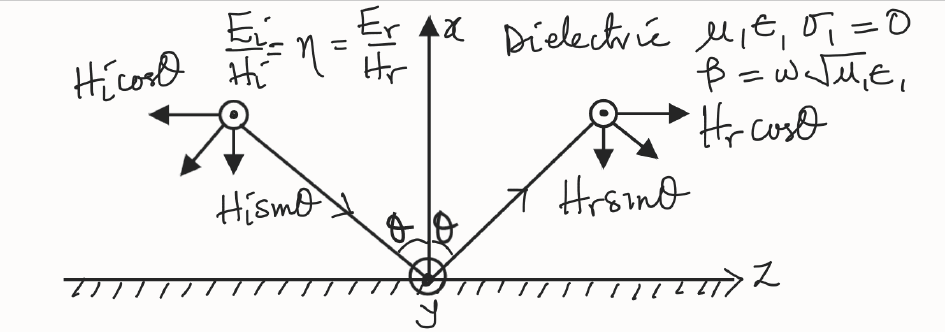
\includegraphics[width=1\linewidth]{./graphics/lec35fig1}
\caption{Incident and reflected electromagnetic wave on a conducting boundary}
\label{fig:lec35fig1}
\end{figure}
The field we had in the dielectric media was a superposition of incident and reflected fields. We obtained an electric field in the medium to be $\bar{E} = \jmath 2E_isin(\beta xcos\theta)e^{-\jmath\beta zsin\theta}$ and $H$ was made up of standing and travelling waves. Here the amplitude of the electric field varies as a sinusoidal pattern in the x-direction perpendicular to the boundary and along the boundary in the z-direction. This is the phenomenon we are going to make use of to get a guiding structure in which electromagnetic energy is not trapped it is travelling in the semi-infinite dielectric medium. If we trap the energy from the two sides we have a parallel plane waveguide. We said the electric field is tangential to the interface at $x=0$, and the tangential component of the electric field should be continuous. We saw that at $x=\frac{m\lambda}{2cos\theta}$, then the electric field at these points becomes zero. Since the electric field had the condition of pointing out or into the paper, i.e. the $\hat{y}$ direction, a conducting sheet placed at $x=\frac{m\lambda}{2cos\theta}$ tangential to this electric field will not affect the boundary conditions. So not only is the tangential component of the electric field 0 at $x=0$ but at some other distance above the interface, the tangential component of the electric field equals zero at $x=\frac{m\lambda}{2cos\theta}$. Hence, the fields which we have got remain unchanged when a conducting sheer is inserted at $x=\frac{m\lambda}{2cos\theta}$. So far $m=0, 1, 2, 3$ we get different values of x at which these boundaries can be inserted without affecting electric or magnetic field distribution. From the graph of variation of $E_y$, $H_x$, and $H_z$ shown in figure~\ref{fig:lec35fig2} with x, we see that at points 1, 2, 3, the field distribution is not affected.
\begin{figure}[h]
\centering
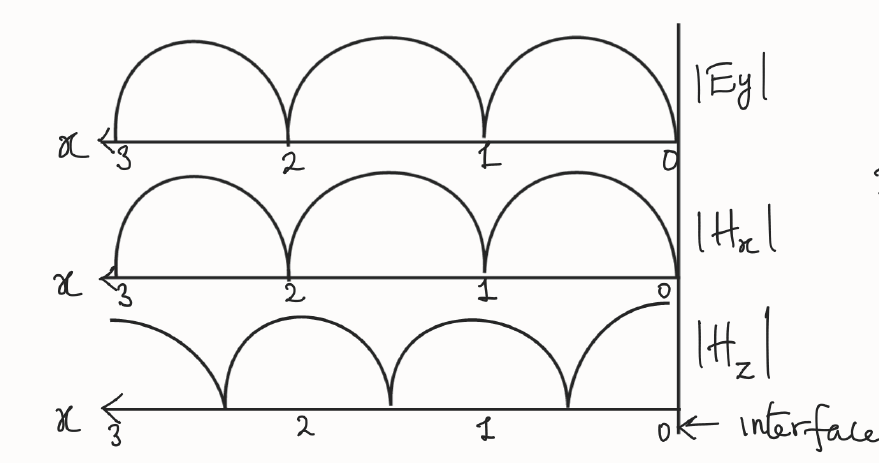
\includegraphics[width=1\linewidth]{./graphics/lec35fig2}
\caption{Variations of components of electric and magnetic fields}
\label{fig:lec35fig2}
\end{figure}

This means that by inserting a conducting sheet at position 1 above the interface, the wave is now trapped between two boundaries. Hence the wave is captured in a form of a closed structure. It is no more a semi-infinite medium. It becomes a bounded medium in the x direction. We can put the conducting plane at 2 or 3 and so on. Here electromagnetic energy is trapped between two parallel planes with a separation between phases given by $x=\frac{m\lambda}{2cos\theta}$. So the new structure is shown in figure|\ref{fig:lec35fig3}. The reflected electric field has the same magnitude as the incident field but goes into the paper contrary to the symbol used for $H$. So we have three components describing the $E$ and $H$ fields. The $E$ field is y oriented, the $H$ has x and z components. The magnetic field is in the xz planes. The electric field (perpendicularly polarized) is oriented tangentially to the plane of incidence. The distance $\frac{\lambda}{2cos\theta}$. So the distance $d=\frac{\lambda}{2cos\theta}$ above the interface, we have the tangential component of the electric field going to zero. At twice this distance $2\left(\frac{\lambda}{2cos\theta}\right)$ from the interface the tangential component of the electric field is zero again. So a place conducting sheet can be placed at any of these distances above the interface plane, without changing the field distribution. When the plane was not at $\frac{\lambda}{2cos\theta}$, fields were distributed at every point above $x>0$. But if a plane conducting sheet is placed at $x=\frac{\lambda}{2cos\theta}$. So we have the propagation of the electromagnetic wave only in the bounded region. So we then have the field surviving in the structure as multiple reflections of the uniform plane wave. They will be bouncing back and forth between the two conducting interfaces or planes. Within these two boundaries with multiple reflections, the wave will travel along the structure or planes.
\begin{figure}[h]
\centering
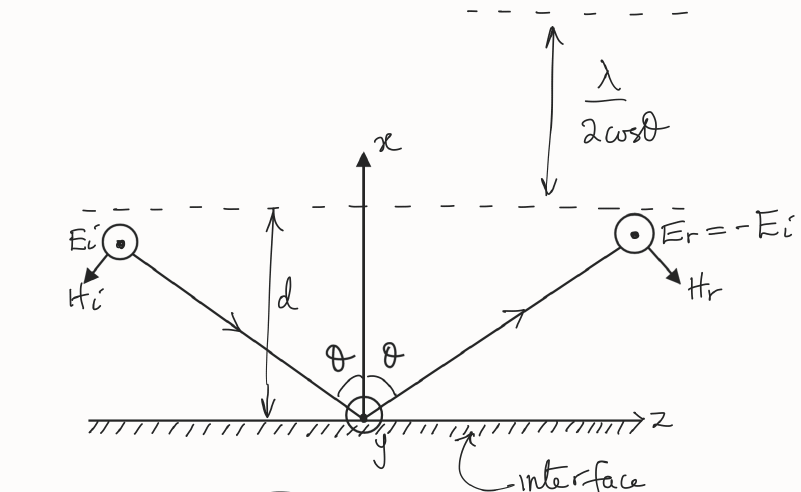
\includegraphics[width=1\linewidth]{./graphics/lec35fig3}
\caption{Incident and reflected electromagnetic wave on a conducting boundary showing the distances when the electric field goes to zero}
\label{fig:lec35fig3}
\end{figure}

Let us invert the problem, i.e. knowing the angle $\theta$, what will be the separation of these planes so that the electric field will not be affected? This is what we have just done. Similarly, given a separation of these two conducting planes as $d$, what angle should the electromagnetic wave be launched such that it can propagate along z or its propagation will be sustained? 
\begin{align*}
d = \frac{m\lambda}{2cos\theta}\\
cos\theta = \frac{m\lambda}{2d}
\end{align*}
$m$ is a discrete number $1, 2, 3, \ldots$. This means that for a given value of d, i.e. a given separation between the two conducting planes, the angel $\theta$ is not continuous, i.e. launching at arbitrary angles which will not sustain the propagation. Only if it is launched at certain angles which are discrete, then and only then can you have a sustained propagation of electromagnetic wave along the structure.

This seems a bit detached from our original understanding of wave propagation in a structure. When we had unbounded media, there was no restriction on the angle, we could launch in any direction. Then in a semi-finite medium (dielectric of the conductor), we could have any angle of incidence and we had semi-field distribution.

\section{Modal Propagation}\index{Modal Propagation}
Now in this case, if we make the structure bound, then an electromagnetic wave cannot be launched at an arbitrary angle of incidence. If we do that, the structure will reject that wave, it will not propagate it. If the wave is launched at the angle which satisfies $cos\theta = \frac{m\lambda}{2d}$ which are discrete angles, then and only then will you have a sustained propagation of what is called a \textbf{Modal Propagation}. So the waves which are launched at discrete angles, superposition of incident and reflected waves will create certain electric and magnetic field patterns within the bound structure. We have a unique pattern created for electric and magnetic fields for a given value of m. For $m=0$, we have a pattern of $E$ and $H$ different form pattern obtained for $m=1$ and so on. $m=1$ gives another pattern of $E$ and $H$ different from that of $m=2$. So we have the discrete electric and magnetic field pattern which can survive inside this bounded structure. This is called \textbf{Modal Propagation} of electromagnetic waves.

So we have migrated now from the continuous domain of $\theta$ to the discrete domain and this is a significant departure we have just encountered in wave propagation. At this point, we can observe a few things, for $\theta$, the $cos\theta$ has to be between 0 and 1, for a given value of $d$, we have a limited number of metres.

When $m$ makes $\frac{m\lambda}{2d}$ greater than 1, that does not represent a physical angle $\theta$. Hence not only that the wave can be launched inside this structure only at discrete angles, we see again that these discrete angles are finite in number. This means that for a given space between the boundaries, only finite numbers of uniform plane waves can be launched given as the number of discrete angles until $\frac{m\lambda}{2d} > 1$.  So this modal propagation is the core of all wave guiding structures whether in parallel, rectangular waveguides, fibre optics etc. Whenever we have a bound medium, the electromagnetic energy is going to travel in definite patterns. That is called a \textbf{Modal Pattern}\index{Modal Patterns} and that propagation is a very important aspect of electromagnetic propagation in a bound structure which is called a waveguide. Once we understand this, finding out the electric and magnetic fields becomes straightforward. So we make some conclusions from all these;
\begin{enumerate}[(i)]
\item Wave survives at discrete angles in a parallel plane waveguide
\item These are a finite number of angles at which the wave survives
\end{enumerate}

With two boundaries, there is nothing like an incident or reflected wave, as an incident wave in one plane is a reflected wave from the opposite plane and vice versa. Depending upon the boundary under consideration, the wave can be called a reflected wave or incident wave.

Hence. with two boundaries, there is nothing like an incident wave or reflected wave as seen in figure~\ref{fig:lec35fig3}. There are two sets of waves which are moving. One set moves up to down (from the top plane to the bottom plane) and another set moves down to up ( from the bottom plane to the top plane). The superposition of these two waves creates a field which is distributed inside the bound structure. This is what is called a \textbf{Modal Pattern}. Shown in figure~\ref{fig:lec35fig4} is what we have essentially with the two sets of waves. The superposition of the fields of these two waves creates the pattern called the modal pattern. Essentially, the propagation of the electromagnetic wave in the bounded structure can be visualized as the superposition of two waves travelling in the pattern shown at an angle with respect to the boundary or perpendicular to the boundary.
\begin{figure}[h]
\centering
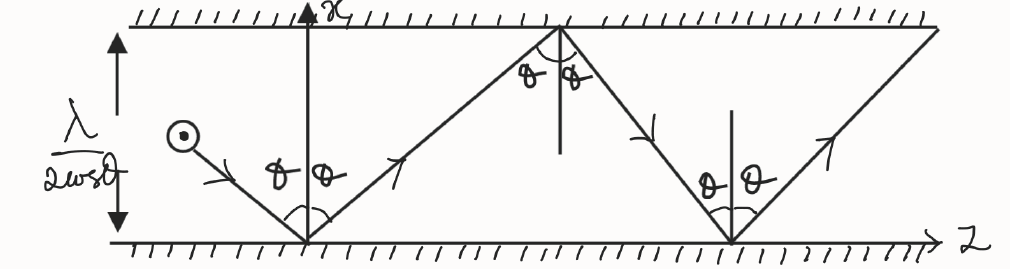
\includegraphics[width=1\linewidth]{./graphics/lec35fig4}
\caption{Wave propagation in a medium of two parallel conducting boundaries}
\label{fig:lec35fig4}
\end{figure}

We observed that in figure~\ref{fig:lec35fig3} with multiple reflections taking place, the net propagation of energy is in the position z direction. The electric field is perpendicular to the plane of incidence i.e. the plane of the paper. So when reflection takes place, the electric field vector maintains the medium. However, the magnetic field direction keeps changing from one point to the other as seen in figure~\ref{fig:lec35fig5}. It shows the direction of $H_i$ and $H_r$ but $E_i$ and $E_r$ remain oriented in the y direction.
\begin{figure}[h]
\centering
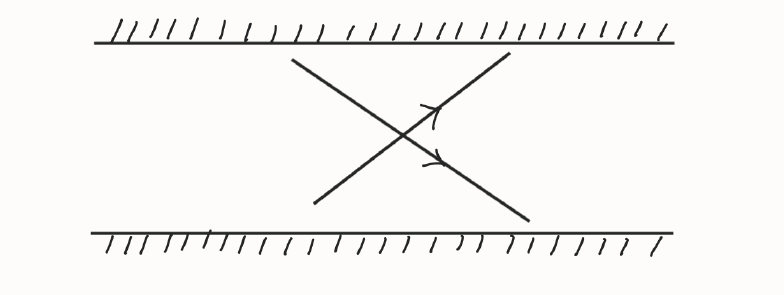
\includegraphics[width=1\linewidth]{./graphics/lec35fig5}
\caption{Wave propagation in a medium of two parallel conducting boundaries showing the superposition of waves}
\label{fig:lec35fig5}
\end{figure}
So $H_r$ and $H_r$ keep changing direction, and the magnetic field inside the plane waveguide has two components, x and z components respectively. Since the net propagation is in the z direction, the magnetic field essentially has components in the direction of net propagation component perpendicular to the direction of net propagation.

Last time
\begin{dmath}
H_x = -\jmath 2\frac{E_i}{\eta}sin\theta sin\left(\frac{m\pi x}{d}\right)e^{-\jmath 2\beta\sqrt{1 - \left(\frac{m\lambda}{2d}\right)^2}}
\end{dmath}
\begin{dmath}
H_z = -\jmath 2\frac{E_i}{\eta}\left(\frac{m\lambda}{2d}\right)cos\left(\frac{m\pi x}{d}\right)e^{-\jmath 2\beta\sqrt{1 - \left(\frac{m\lambda}{2d}\right)^2}}
\end{dmath}
These are the three fields which can survive in a particular waveguide for a perpendicularly polarized electric field (perpendicular to the plane of incidence). Now the phase constant for the mode is
\begin{dmath}
\bar{\beta} = \beta\sqrt{1 - \left(\frac{m\lambda}{2d}\right)^2}
\label{eqn:phaseconst}
\end{dmath}
This is the phase constant as a result of the superposition of two uniform plane waves in the z-direction. $\beta$ is just the phase constant of a single wave moving into the medium.
\begin{dmath}
sin\theta = \sqrt{1-\left(\frac{m\lambda}{2d}\right)^2} 
=\frac{\bar{\beta}}{\beta}
\end{dmath}
The first thing we immediately note from these three expressions is if we put $m=0$, then the electric field goes to zero, $H_x$ goes to zero, and $H_z$ goes to zero. This means that for the fields to survive inside this structure, we must have values of m which is a non-zero integer. Since for $cos\theta = 0$ or $\theta = 90^o$. That means the wave incident on the waveguide cannot survive inside this structure. So if we launched a wave with the electric field shown in figure~\ref{fig:lec35fig6} and with the direction in the y-direction, the wave cannot survive. $E$ is perpendicular to the paper, with $m=0$, the wave cannot survive. 
\begin{figure}[h]
\centering
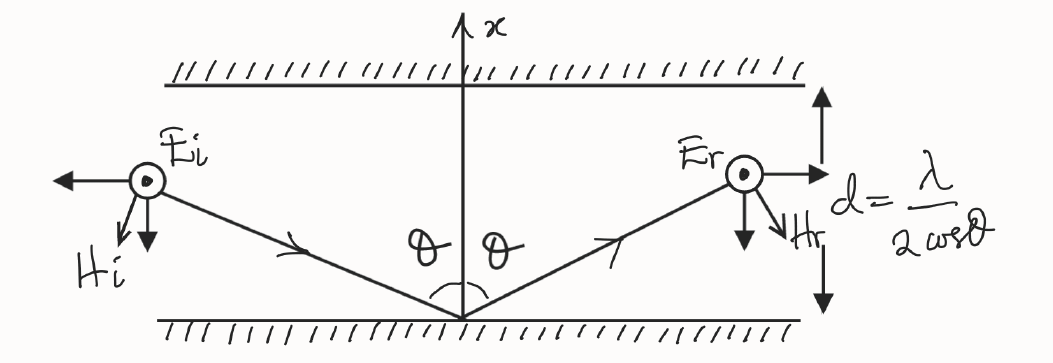
\includegraphics[width=1\linewidth]{./graphics/lec35fig6}
\caption{Wave propagation in a parallel plane waveguide with distance set to $\frac{\lambda}{2cos\theta}$}
\label{fig:lec35fig6}
\end{figure}
Why does this happen? We can see physically from the waveguide structure, m essentially tells us that at $m=1$ and $x=0$ to $d$, we get $\dfrac{1}{2}$ cycle variation of the electric field. So we get the amplitude variation of $E$ shown in the figure~\ref{fig:lec35fig7} for $m=1$, for $m=2$, we have a full cycle variation\footnote{Wondering how it was found, here it is.

At $x=\dfrac{d}{2}$,
\begin{dmath*}
sin\left(\frac{m\pi x}{d}\right) = sin\left(\frac{m\pi \dfrac{d}{2}}{d}\right) = sin\pi = 0
\end{dmath*}}, and for $m=3$, we have $1\dfrac{1}{2}$ cycle variations. 
\begin{figure}[h]
\centering
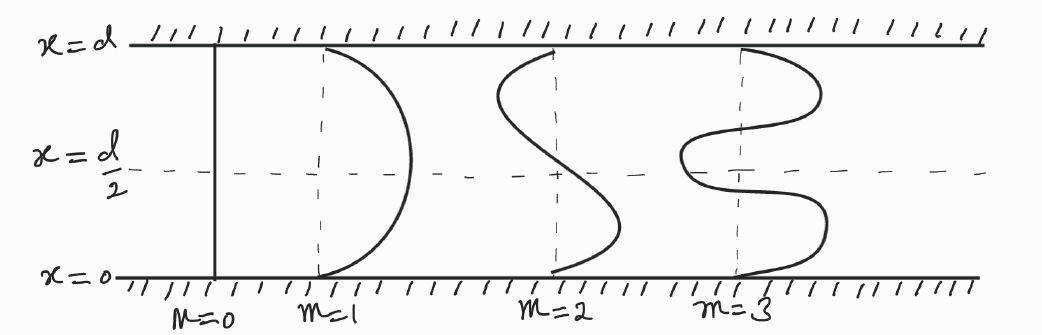
\includegraphics[width=1\linewidth]{./graphics/lec35fig7}
\caption{Electric Field variation with different values of $m$}
\label{fig:lec35fig7}
\end{figure}

So m tells us how many half cycles variations of the electric field amplitude or magnetic field amplitude in the direction transverse to the direction of net wave propagation. So if $m=0$, there is no variation which means a constant field from $x=0$ to $x=d$. $m=1$ means 1 half-cycle variation, $m=2$ means 2 half-cycle variations, $m=3$ means 3 half-cycle variations and so on. For $m=0$ the field is constant in the direction transverse to the direction of propagation. Since the electric field is in the y direction, between two conducting planes, at the conducting boundaries, the electric field must be zero at both of them. For $m=0$ we do not want any variation of the field and it should be zero at $x=0$ and $x=d$.That will only happen if the field is identically zero everywhere. That is what the bold part of the expression, $\bar{E} = \jmath 2E_i\boldsymbol{sin\left(\frac{m\pi x}{d}\right)}e^{-\jmath 2\beta\sqrt{1 - \left(\frac{m\lambda}{2d}\right)^2}}$, tells us. So the lowest value of m which can survive in the structure is $TE_1$ mode. Hence, for a given spacing of conducting planes, we must have a value, m, which is at least 1 and only then will the field exist in the structure, if $m=0$ the field will not exist inside the structure and the wave will not propagate. So depending upon the size or mode, we can have $TE_1$, if the size is sufficient, $TE_2$, $TE_3$ and so on.

On a given structure, we can have multiple modes propagating depending upon how the angles $cos\theta = \frac{m\lambda}{2d}$ can be satisfied. $m=1$ is the lowest mode, so the question is what wave can survive in mode 1? With $cos\theta = 1$, $\dfrac{m\lambda}{2d} = 1$, hence, $\lambda = 2d$ or $d = \dfrac{\lambda}{2}$. This implies that the separation between the planes is $\dfrac{\lambda}{2}$. Thus in $TE_1$ mode the smallest separation is $\dfrac{\lambda}{2}$, if it is less than $\dfrac{\lambda}{2}$, we cannot have an angle as $\dfrac{m\lambda}{2(0.4\lambda \text{ assume})}> 1$, so that $cos\theta > 1$. No physical angle has its cosine greater than 1. So the lowest mode for which the wave can propagate in the structure has $d \geq \dfrac{\lambda}{2}$\footnote{This makes $cos\theta \leq 1$}. So not only that the separation distance $d$ is given, but a wavelength is required for which $d\geq\dfrac{\lambda}{2}$ or inverted $\lambda \leq 2d$. This means the frequency has to be above certain values so that $\lambda \leq 2d$ is satisfied, only then will the wave propagation take place. If $\lambda > 2d$ or frequency is less than certain values, then wave propagation cannot take place inside the structure.

\section{Trough of a mode}\index{Trough of a mode}
 So from here, we get an important concept of what is called the \textbf{Trough} of a mode, that is when $d = \dfrac{\lambda}{2}$ or $\lambda = 2d$ which is the lowest frequency that can propagate on a waveguide whose separation is $d$.
\begin{dmath}
\lambda_{max} = 2d
\label{eqn:cut-offlambda}
\end{dmath}
\begin{dmath*}
\frac{c}{f_{min}} = 2d
\end{dmath*}
\begin{dmath}
f_{min} = \frac{c}{2d}
\label{eqn:cut-offf}
\end{dmath}
Equations \ref{eqn:cut-offlambda} and \ref{eqn:cut-offf} are the maximum wavelength and minimum frequency respectively that defines wave propagation. Below $f_{min}$, the wave doesn't propagate and that is the minimum frequency for $m=1$ mode and it is called the cut-off frequency of that mode. So for a particular mode to propagate the frequency must be above that value and that is called the cut-off frequency for that mode.

The cut-off frequency is the lowest frequency which would propagate inside the structure for a given mode number or given $m$. Either we see that or the mode increases to $TE_2$, the frequency will be doubled and so on. Hence the reason we say the lowest mode is because that is the lowest frequency in the structure which can propagate.

Substituting $d=\dfrac{\lambda}{2}$ and $m=1$ in equation ~\ref{eqn:phaseconst} gives:
\begin{dmath*}
\bar{\beta} = \beta\sqrt{1 - \left(\frac{m\lambda}{2d}\right)^2} =  \beta\sqrt{1 - \left(\frac{\lambda}{2\left(\frac{\lambda}{2}\right)}\right)^2} = 0
\end{dmath*}
This shows that the frequency at $d=\dfrac{\lambda}{2}$ which is the cut-off frequency, the phase constant of the wave goes to zero. Below this frequency $\left(\dfrac{m\lambda}{2d}\right)^2 > 1$, the expression $\sqrt{1 - \left(\frac{m\lambda}{2d}\right)^2}$ in the phase constant is imaginary, so $\bar{\beta}$ becomes imaginary. It is no more a phase constant but becomes an attenuation constant i.e. the wave losses its wave nature in the presence of a field which is dying down exponentially. So below the cut-off frequency, it represents a field which is exponentially decaying and hence no propagation of electromagnetic waves.

What we see from this analysis is that when we have a band structure like a parallel plane waveguide, first there are the discrete angles at which uniform plane waves are bouncing back and forth between two parallel planes giving the field distribution and those field patterns we call modal patterns. We also see that for a given mode number, the frequency has to be above certain values called cut-off frequency for that mode. So depending on the mode you want to excite, you require a certain frequency. So even if the waveguide is capable of supporting the different values of $m$, it would depend on the frequency whether the wave will be accepted or not i.e. if the frequency is greater than the cut-off frequency or not. This is the basic picture of modal propagation within a bounded structure like a waveguide. We will elaborate on this and then following this, we will try to see other modes and then move on to complex structures like the rectangular waveguides.
% \chapter{Propagation of electromagnetic wave inside a parallel plane waveguide (2)}
We continue with our investigation of the propagation of electromagnetic waves inside a parallel plane waveguide. i.e two conducting boundaries with waves moving in between them. In the previous chapter, we launched a wave which had perpendicular polarization between two conducting boundaries; as a result, we get a propagation which we call transverse electric propagation.

We introduced the concept of mode i.e the discrete electric and magnetic field patterns which propagate between these two conducting boundaries. What if we use a parallel polarized electric field instead of perpendicular polarization? What kind of propagation will take place and how does it differ from the previous case of perpendicular polarization? Figure~\ref{fig:silas1} shows a conductor boundary with the incident and reflected wave. The coordinate system is shown with y pointing out of the paper and as such the electric field is directed in the plane of the paper. Since this is a transverse wave, by Poynting theorem, the magnetic field for both must be in the y direction.
\begin{figure}[h]
\centering
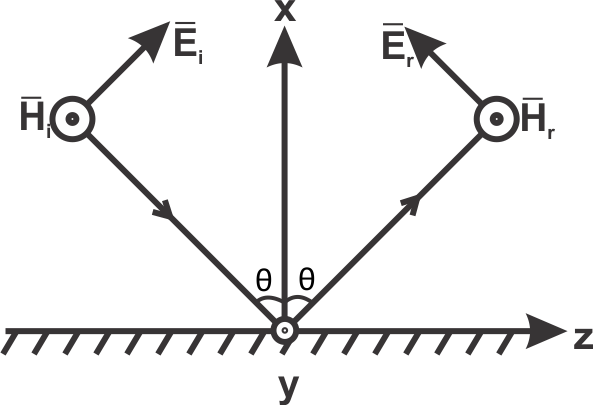
\includegraphics[scale=1]{./graphics/silas1}
\caption{Incident and reflected wave on a boundary that lies in the z plane}
\label{fig:silas1}
\end{figure}
The problem is identical to what we had in the previous case. We find out the component of electric and magnetic fields and apply the boundary conditions.
\begin{figure}[h]
\centering
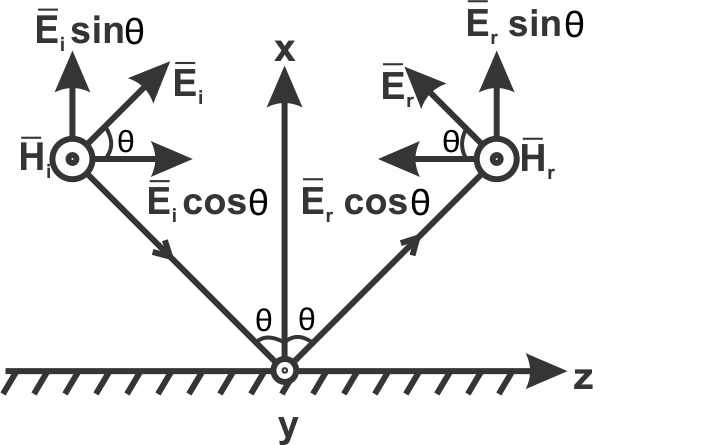
\includegraphics[scale=1]{./graphics/silas2}
\caption{Incident and reflected wave with projected electric fields in the rectangular coordinate system}
\label{fig:silas2}
\end{figure}
At x = 0, the tangential component of the electric field should be zero.
\begin{equation*}
\bar{H_{i} = H_{i} e^{-j\beta(-xcos\theta + zsin\theta)} \hat{y}}
\end{equation*}
\begin{equation*}
\bar{H_{r} = H_{r} e^{-j\beta(-xcos\theta + zsin\theta)} \hat{y}}
\end{equation*}
\begin{equation*}
\bar{E_{i} = E_{i} e^{-j\beta(-xcos\theta + zsin\theta)} \hat{y}}
\end{equation*}
\begin{equation*}
\bar{E_{r} = E_{r} e^{-j\beta(-xcos\theta + zsin\theta)} \hat{y}}
\end{equation*}
Taking the component of the incident electric field in the z direction, we have $E_{i} cos\theta$ and $-E_{r}cos\theta$ for the reflected electric field in the z-direction also.\\
$E_{iz} = E_{i}cos\theta e^{-j\beta(-xcos\theta + zsin\theta)}$	for the boundary condition and x = 0\\
$E_{rz} = -E_{r}cos\theta e^{-j\beta(xcos\theta + zsin\theta)}$   Sum of tangential electric field is zero.\\
At x = 0, $E_{ton} = E_{iz} + E_{rz}$\\
If we substitute, we have\\
\begin{equation*}
E_{i}cos\theta e^{-j\beta(-xcos\theta + zsin\theta)} - E_{r}cos\theta e^{-j\beta(xcos\theta + zsin\theta)} = 0
\end{equation*}
as x$\rightarrow$
\begin{equation*}
E_{i}cos\theta e^{-j\beta(zsin\theta)} - E_{r}cos\theta e^{-j\beta(zsin\theta)} = 0
\end{equation*}
\begin{align*}
E_{i} = E_{r}\\
\Gamma= 1 = \frac{E_{i}}{E_{r}}
\end{align*}
We recall that we have a reflection coefficient $\Gamma = -1$ in the case of perpendicular polarization. This means it was behaving like a short circuit. For the parallel polarization, the transmission line analogy is an open circuit? which is not correct. The $E_{i}$ and $E_{r}$ from the diagram have a direction opposite to each other. So that in the case of perpendicular polarization, the $E_{i}$ and $ E_{r}$  were initially taken to be in the positive y direction. So   $\Gamma = 1$ means they are opposite to one another in direction, so n = -1 corresponded to the case of a short circuit in Transmission lines. Hence the negative sign that could have been in $\Gamma$ here is already taken care of by making $E_{i}$ and $E_{i}$ have opposite directions in the case of parallel polarization considered here. Thus, the reason the reflection coefficient is 1. 

Looking at the sign of the reflection coefficient alone will not give the correct idea about the boundary. In summary, this parallel polarized case is still behaving like a short circuit, where the conductivity is infinite. The electric field is zero at the boundary, you get a reflection coefficient of +1 because the sign is appropriately absorbed into the direction of the electric field. Once you get that and use the relationship that the electric field is related to the magnetic field by the intense importance, we have $\frac{E_{i}}{H_{i}} = \frac{E_{r}}{H_{r}} =\Gamma$. The total electric field in medium 1 is a summation of the incident and reflected field. The same is true for the magnetic field. The electric field has two components in x and z, the magnetic field has components in only y duration. The magnetic field will have only the y component.
\begin{equation*}
E_{i}sin\theta e^{-j\beta(-xcos\theta + zsin\theta)} + E_{r}sin\theta e^{-j\beta(xcos\theta + zsin\theta)}
\end{equation*}
$E_{i} =E_{r}$    since $\Gamma =1$\\
we have
\begin{dmath*}
E_{r}sin\theta [e^{-j\beta(-xcos\theta} + e^{-j\beta cos\theta}] e^{-j\beta(zsin\theta)} = 2E_{i}sin\theta cos(\beta xcos\theta)
\end{dmath*}
therefore,
\begin{dmath*}
E_x = 2E_{i}sin\theta cos(\beta xcos\theta)
E_{2} is E_{i}cos\theta e^{-j\beta(-xcos\theta + zsin\theta)} - E_{r}cos\theta e^{-j\beta(xcos\theta + zsin\theta)} 
\end{dmath*}
\begin{dmath*}
= E_{i}cos[e^{j\beta xcos\theta} - e^{-j\beta xcos\theta}]e^{-j\beta zsin\theta}
=2jE_{i}e^{-j\beta zsin\theta} cos\theta \times sin(\beta xcos\theta)
\end{dmath*}
The magnitude field will have only y component
\begin{equation*}
H_{y} = H_{i}e^{-j\beta(-xcos\theta + zsin\theta)} + H_{r}e^{-j\beta(+xcos\theta + zsin\theta)}
\end{equation*}
since $\Gamma = 1 that is E_{i}=E_{r}$
\begin{equation*}
= \frac{E_{i}}{\eta} e^{-j\beta(-xcos\theta + zsin\theta)} + \frac{E_{i}}{\eta}e^{-j\beta(+xcos\theta + zsin\theta)}
\end{equation*}
\begin{equation*}
=\frac{E_{i}}{\eta} e^{-j\beta(-zsin\theta)} [e^{j\beta xcos\theta} + e^{-j\beta xcos\theta}]
\end{equation*}
\begin{equation*}
= 2\frac{E_{i}}{\eta} cos(\beta xcos\theta)e^{-j\beta zsin\theta}
\end{equation*}
So we have the three equations
\begin{equation}
E_x = 2 E_{i} e^{-j\beta zsin\theta} sin\theta cos(\beta xcos\theta)
\label{eqn:field1}
\end{equation}
\begin{equation}
E_z = 2 jE_{i} e^{-j\beta zsin\theta} sin\theta cos(\beta xcos\theta)
\label{eqn:field2}
\end{equation}
\begin{equation}
H_y = 2 \frac{E_{i}}{\eta} cos(\beta xcos\theta) e^{-j\beta zsin\theta} 
\label{eqn:field3}
\end{equation}
If we look at the tangential component of the electric field $E_{2}$, this is going to be zero at x = 0. That is when $sin(\beta xcos\theta) =0$ or $\beta xcos\theta = m\pi$ where m = 0,1,2.... The angle at which the parallel polarization can be launched to propagate the wave becomes discrete angles given as $cos\theta = \frac{m\pi}{\beta x}$. If the separation between the conducting plane 'x' is given, i.e. x = d, then we can launch the wave at discrete angle =0 for m=0,1,2,3... Whether we take a parallel polarization, the angles at which the wave can be launched inside the structure remain the same for either case. All the arguments we have in the previous case like you have a finite number of angles in which the wave can be launched, and the minimum value of frequency required, all those arguments are applicable here too. With waveguide separation $d$, $cos\theta$ = $\frac{m\pi}{\beta d}$.
%\begin{figure}[h]
%\centering
%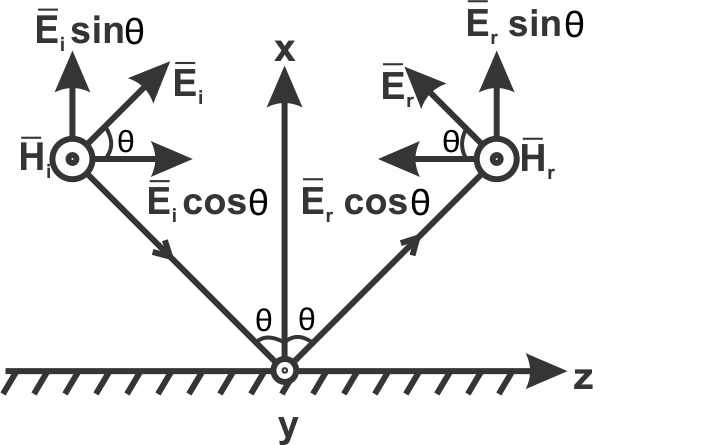
\includegraphics[scale=1]{./graphics/silas2}
%\caption{}
%\end{figure}
From figure~\ref{fig:silas2}, the magnetic field component is always perpendicular to the plane of incidence, while the electric field i.e. on the plane of the paper. $cos(\beta xcos\theta)$ represents an expression for a standing wave in the x-direction and $e^{-j\beta zsin\theta}$ gives a travelling wave behaviour in the z-direction. So in this case our field will travel in the z-direction, with a phase constant $\beta sin\theta$. So a field parallel is generated also if a conducting wave is placed at distance $d= \frac{m\lambda}{z cos\theta}$, that is travelling with a phase constant $\beta sin\theta$ in the z-direction. Since the wave is travelling in the z-direction and the magnetic field is now perpendicular to the direction of travel along all points within these two conducting boundaries, the magnetic field is always transverse to the direction of no propagation of the electromagnetic wave. This mode is called a \textbf{Transverse Magnetic} mode or TM mode.

\section{Tranverse Magnetic  Modes ($TM_m$)}\index{Transverse Magnetic Modes}
 Following the convention, $m$ defines the order of the mode i.e. tells us how many no of half cycles variation we have from $x = 0$ to $x = d$.
\begin{figure}[h]
\centering
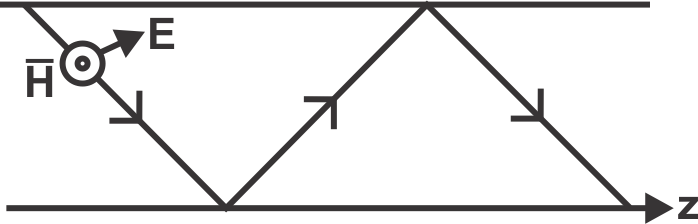
\includegraphics[scale=1]{./graphics/silas3}
\caption{Transverse magnetic  mode}
\end{figure}
Hence, $ m = 1$ means 1 half-cycle variation between $x = 0$ and $x = d$, $m = 2$ means 2 half-cycle variations between $x = 0$ and $x = d$, and when $m = 0$, the fields are constant with no variation. This is represented as $TM_m$. 

For a given value of $d$, the value of $m$ we choose to execute the fields will decide the order of the mode of propagation. Now we see that we have two types of propagation inside a parallel plane waveguide. The transverse electric mode $TE$ and the transverse magnetic mode $TM$ for which electric and magnetic field remains transverse to the direction of net wave propagation respectively. 

Up till now, the behaviour is very identical. They have the same condition satisfied for the electric field, but the magnetic and electric field expressions are different. Otherwise no difference between $TE$ or $TM$ modes. With $x = d$,
\begin{dmath*}
cos\theta = \frac{m \pi}{\beta d} =\frac{m \pi}{\frac{2\pi d}{\lambda}} = \frac{m\lambda}{2d}
\end{dmath*} 
or
\begin{dmath*}
\beta cos\theta = \frac{m \pi}{d}
\end{dmath*}
We substitute for $\beta cos\theta$ in the field equations \ref{eqn:field1}, \ref{eqn:field2}, and \ref{eqn:field3}.
\begin{dmath}
E_{x} = 2 E_{i} e^{-j\beta zsin\theta} sin\theta cos(\beta xcos\theta) = 2 E_{i} e^{-j\beta zsin\theta} sin\theta cos(\frac{m\pi x}{d})
\end{dmath}
\begin{dmath}
E_{2} = 2 jE_{i} e^{-j\beta zsin\theta} sin\theta cos(\beta xcos\theta) = 2 jE_{i} e^{-j\beta zsin\theta} sin\theta cos(\frac{m\pi x}{d})
\end{dmath}
\begin{dmath}
H_{y} = 2 \frac{E_{i}}{\eta} cos(\beta xcos\theta) e^{-j\beta zsin\theta} =2 \frac{E_{i}}{\eta} cos(\frac{m\pi x}{d}) e^{-j\beta zsin\theta} 
\end{dmath}
Again, $m$ gives the number of half-cycle variations between $x = 0$ and $x = d$. In the transverse electric case with $m = 0$, ALL THE FIELDS BECAME ZERO. Thus, the $TE_0$ mode cannot exist inside a parallel plane waveguide. In this case if we put $m = 0$, then $cos\theta =0$, $\theta =90$, that means $sin\theta =1$. The wave will move parallel to the conducting boundary. In this case of $m = 0$, $cos\theta =0$ and $sin\theta =1$ and $\theta=\frac{\pi}{2}$ , so we have for $TM_0$\\ 
$E_{x} =2E_{i} e^{-j\beta z}$, $E_{z}= 0$, $H_{y} =\frac{2E_{i}}{\eta} e^{-j\beta z}$.

Here the phase constant is the same as we have for the intrinsic medium filling the parallel plane waveguide. We notice that when $m = 0$, all the fields do not identically go to zero. That means $TM_0$ mode does exist so contrary to $TE_0$ mode which does not exist, and subsequently, we have $TM_{1}$, $TM_{2}$, and so on. 

\section{Phase and Group Velocities}\index{Phase and Group Velocities}
Phase constant in the z-direction is
\begin{dmath*}
\bar{\beta} = \beta sin\theta = \beta \sqrt{1- cos^{2}\theta} =\sqrt{\beta^{2} -\beta^{2}cos\theta} = \sqrt{\beta^{2} -\frac{m\pi}{d}^{2}}
\end{dmath*}
This is the phase constant for the transverse magnetic case, with $m = 0$, $\bar{\beta}$ reduces to $\beta$ here. With $m\neq 0$, we can ask with what velocity this particular mode will be travelling. Thus, we define velocity by group velocity $v_{g}$ or by phase velocity $v_{p}$. 
\begin{dmath}
 v_{p}=\frac{\omega}{\bar{\beta}} =\frac{\omega}{\beta \sqrt{1- \frac{m \pi}{\beta d}^{2}}}
\label{eqn:phasevel}
\end{dmath}
$\beta$ is the phase constant in the medium filling the two conducting planes, $\frac{\omega}{\beta}$ is the velocity of a wave in an unbound medium having the same property, and $\frac{\omega}{\beta}$ is the velocity of light, $c$. Thus equation~\ref{eqn:phasevel} becomes;
\begin{equation*}
v_{p} =\frac{c}{\sqrt{1-(\frac{m\lambda}{2d})^{2}}}
\end{equation*}
\begin{align*}
\beta =\frac{2\pi}{\lambda}\\
\frac{\pi}{\beta} =\frac{\lambda}{2}
\end{align*}
but 
\begin{align}
v_{p} v_{g}= c^{2}
\label{eqn:grpvel}
\end{align}
$v_{g}$ is the group velocity. In the parallel plane waveguide shown in figure~\ref{fig:silas4}, with the wave going at an angle $\theta$, the component of the wave in the z-direction gives the group velocity of the wave in the z-direction in the parallel plane waveguide. The velocity of the wave in the $\theta$ direction is $c$. So that $c\times cos(\frac{\pi}{2} - \theta)= c\times sin\theta= v_{gz}$. The group velocity is the component of the velocity in the z-direction.
\begin{figure}[h]
\centering
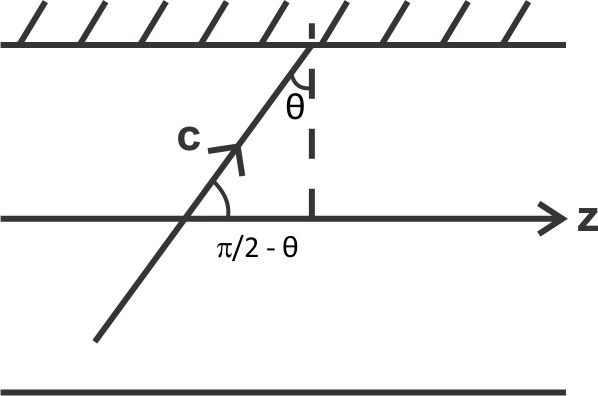
\includegraphics[scale=1]{./graphics/silas4}
\caption{Group velocity of a wave propagating in a medium bounded by a parallel plane in the z plane}
\label{fig:silas4}
\end{figure}
From equation~\ref{eqn:grpvel}, we can derive the group velocity as:
\begin{dmath*}
v_g = \frac{c^2}{v_p} = \frac{c^2}{\frac{c}{sin\theta}}= c\sqrt{1-cos^{2}\theta} =c\sqrt{1-(\frac{m\lambda}{2d})^{2}}
\end{dmath*}
The group velocity is the velocity of the energy. We note two things from these expressions, if $m \neq 0$, the phase velocity is a function of wavelength. For a given mode,$m \neq 0$ when the frequency changes, the phase velocity of that particular mode changes. The property of velocity of a wave changing as a function of frequency is called \textbf{Dispersion}\index{Dispersion}. 

\subsection{Dispersion}
What we find is when we have a medium like this parallel plane waveguide, the structure has become a dispersive structure. This is when electromagnetic wave tires move in the structure, the velocity becomes a function of frequency or function of wavelength. So though the medium feeling this waveguide is not dispersive, the conducting boundary or dial conductors we talked about are not also dispersive, but this bound medium has become a dispersive medium. When we have a bounded structure, in general, we may expect dispersion on the bound structure i.e. their velocity varies as a function of frequency. Hence, neither the medium within the conductor nor the conducting plane itself is dispersive, but the \textbf{Bounded Structure} formed with all these have become \textbf{Dispersive}.
\begin{equation}
\bar{\beta} = \sqrt{\beta^{2} -\left(\frac{m\pi}{d}\right)^{2}}
\end{equation} 
This is called the \textbf{Dispersion Relation} for a particular mode, it tells the variation of velocity as a function of frequency or wavelength. The conclusion is that whenever we have a bound structure, the velocity varies as a function of frequency or wavelength.

$(\frac{m\lambda}{2d})^{2} -1=0$ gives the cut-off wavelength, and at $\beta^{2} -(\frac{m\pi}{d})^{2}$, the wave propagation will stop. For a frequency lower, wave propagation does not take place and for a higher frequency than $f_{cut-off}$, the wave propagates. As we approach cut-off frequency, $v_{p}\Rightarrow \infty$ i.e $v_{p}= \frac{c}{\beta \sqrt{1- \frac{m \lambda}{2d}^{2}}}$ at cut-off $1 - (\frac{m\lambda}{2d})^{2}=0$ $v_{p} =\frac{c}{0} =\infty$

$v_{g} =c \sqrt{1-(\frac{m\lambda}{2d})^{2}}$ $\Rightarrow 0$. With $v_{g} = 0$ it means at cut-off, the energy flow stops. At frequencies very high compared to cut-off frequencies, $\lambda$ becomes very very small compared to cut-off, $\frac{m\lambda}{2d} \rightarrow 0$ becomes negligibly small,$v_{g} \approx c$, $v_{p} \approx c$. so at higher frequencies compared to cut-off frequency, $v_{g}$ and $v_{p}$ approaches the intrinsic velocity in the medium.
\begin{figure}[h]
\centering
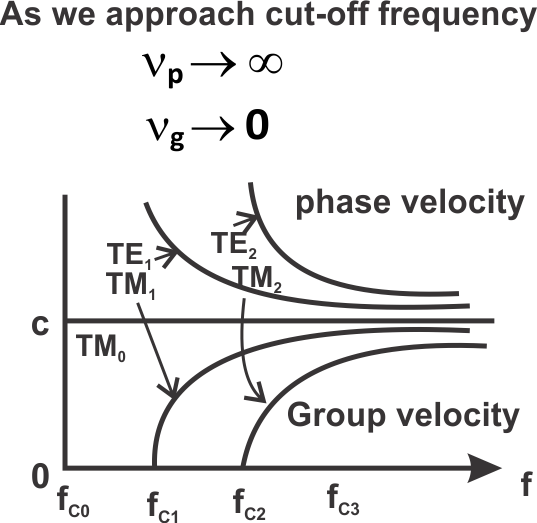
\includegraphics[scale=1]{./graphics/silas5}
\caption{Group and phase velocities versus frequency at different $TE$ and $TM$ modes}
\label{fig:silas5}
\end{figure}
A plot of group and phase velocity for different frequencies is shown in figure~\ref{fig:silas5}. $f_{c1}$ is the cut-off frequency for mode $m=1$, $f_{c2}$ is the cut-off frequency for mode $m=2$, $f_{c0}$ is the cut-off frequency for mode $m=0$ which exists for only $TM$ since $TE_0$ does not exist.

From equation~\ref{eqn:phasevel}, we can see that if $m=0$, $v_{p} =c$ ($TM_o$ since $TE_o$ does not exist). For $m=1$
\begin{equation*}
v_{p}= \frac{c}{\beta \sqrt{1- \frac{\lambda}{2d}^{2}}}
\end{equation*}
As $v_{p} \Rightarrow c$, starting from $\infty$ at $f_{c1}$, $v_{g} \Rightarrow c$ starting from 0 at $f_{c1}$.
\begin{equation*}
v_{g}= c\sqrt{1-\left(\frac{\lambda}{2d}\right)^{2}}
\end{equation*}
At cut-off frequency, 
\begin{align*}
1-\left(\frac{m\lambda}{2d}\right)^{2} = 0
\end{align*}
Therefore, at every cut-off for the respective mode, $v_{p}$ starts from $\infty$ and tends to $c$ as $f$ increases, $v_{g}$ starts from 0 and approaches $c$ as f increases. $TM_{1}$, and $TE_{1}$, do exist, But $TE_0$ does not exist when $TM_0$ exists. For $m = 0$, $v_{p}=c$ $v_{g}=c$. The phase velocity is always above $c$ and the group velocity is always below $c$.

The graph in figure~\ref{fig:silas5} shows the group and phase velocity plot for the different modes, where $f_{c0}$, $f_{c1}$, and $f_{c2}$ are the cut-off frequencies for the different modes. For the $TM_0$ mode, there is no cut-off frequency because $\bar{\beta}$ is always equal to $\beta$ which is the phase constant in the intrinsic medium. With this understanding we go back to all the special cases we have talked about. Recall with $m = 0$, 
\begin{align*}
E_{x} =2E_{i} e^{-j\beta z}\\
H_{y} = \frac{2E_{i}}{\eta} e^{-j\beta z}\\
H_{z} =0
\end{align*}
This is the $TM_0$ mode. For the $TM_0$ mode, we draw the parallel plane waveguide to illustrate it $\theta =90^{0}$ means the wave is launched parallel to the interface as shown in figure~\ref{fig:silas6}

\section{Transverse Electromagnetic Mode $TEM$}\index{Transverse Electromagnetic Mode}
\begin{figure}[h]
\centering
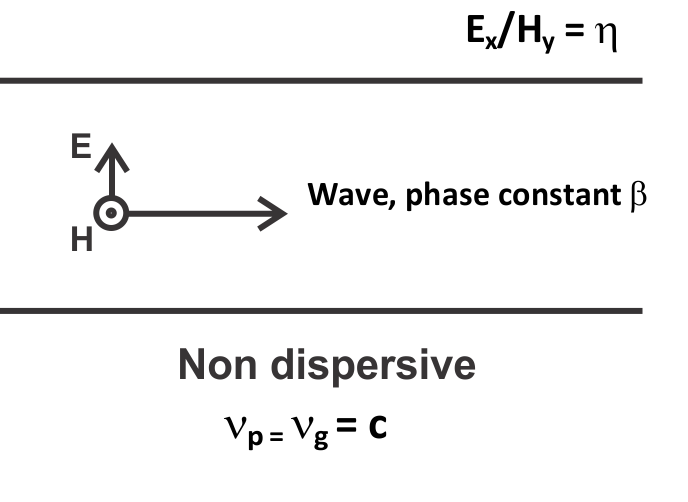
\includegraphics[width=1\linewidth]{./graphics/silas6}
\caption{Wave propagation in $TM_0$}
\label{fig:silas6}
\end{figure}
The electric field is x-oriented, and the magnetic field is y-oriented i.e. pointing out of the plane of the paper. The wave is propagating in the z-direction with a phase constant $\beta$. We note that $\frac{E_{x}}{H_{y}} = \eta$. We see that in this case, the electric and magnetic field is now perpendicular to the direction of wave propagation z, $E_{x}\perp z$,$H_{y}\perp z$, and $E_{x}\perp H_{y}$. Hence the $TM_0$ mode is a case of \textbf{Transverse Electromagnetic Wave} and so we can call it a $TEM$ mode (Transverse Electromagnetic mode). $TM_0$ mode from here makes the electric and magnetic field becomes transverse to the direction of propagation hence the reason it is called Transverse Electromagnetic mode (TEM). With $\frac{E_{x}}{H_{y}} = \eta$ it means we are having a transverse electromagnetic wave posing in between the two planes. It has all the properties a uniform plane wave has in an unbound medium.

A question that comes to mind is if the conducting boundary still has any effect on the wave propagation, since if the boundaries are not there the wave would have travelled like a transverse electromagnetic wave. When the wave is launched the way it is shown in figure~\ref{fig:silas6} with the electric field perpendicular to the boundary, there is no boundary condition on normal components of the electric field. The normal component of the electric field always tends to be balanced by surface charges on the conducting boundary. Similarly, if we have a tangential component of the magnetic field we can have surface circuits on the conducting boundary. This balances out the tangential magnetic field in the conducting boundary. Now we can have a uniform magnetic and electric field, the wave passes through the parallel plane waveguide as if the boundaries are not modifying the electric and magnetic fields. whichever electric and magnetic field we have, they can induce appropriate surface changes and current, and this field does not get modified. Hence this $TM_0$ mode propagates in a parallel plane waveguide, and since $m = 0$, this mode is \textbf{Non-dispersive}. That means for this mode, the velocity $v_{p}=v_{g}=c$. The cut-off frequency for this mode is zero as we have seen when m = 0. That means this mode can propagate down to zero frequency. Precisely, this is what we see when we are having a two-conductor plane system, any lowest possible frequency voltage can be applied to the system and the energy would still be transferred or transported. However, higher-order modes require a minimum frequency for transporting the energy. So we find that in a parallel plane waveguide, this $TM_0$ mode also called a TEM mode is a mode that propagates at the lowest frequency. As we go to higher frequencies, we require higher other modes or we get higher order modes in the energy propagation.

% \chapter{Analysis of waveguide general approach}
In previous chapters, we investigated a structure called a parallel plane waveguide. If we are having two conducting boundaries, we saw that the electromagnetic energy can propagate between these two boundaries in the form of some definite electric and magnetic field patterns which are called modes. We also try to visualize the propagation of electromagnetic waves between these two boundaries as a superposition of uniform plane waves.

This understanding of modal propagation in terms of the uniform plane wave gives you a correct picture of how the modes are established inside a waveguide. However, this approach that visualises a modal pattern in terms of the fields of a uniform plane wave is always not as easy as we saw in terms of the parallel plane waveguide. In a parallel plane waveguide, since the medium still was infinite at least parallel to the conducting boundaries, we still could use or visualize the uniform plane wave propagating between the boundaries.

However, if we have a structure, like a pipe kind of structure; whether a rectangular pipe or circular pipe or a pipe of arbitrary shape and if I want to find out how the electromagnetic energy is going to propagate inside this structure, it will be extremely difficult to visualize the propagation in terms of a superposition of uniform plane wave and those situations. We develop a mathematical framework and try to solve the problem of electromagnetic wave propagation in structure using that general mathematical formulation.

In this chapter, we develop a general framework for analyzing wave propagation inside an arbitrary waveguide. And then, whatever result we get mathematically, we will try to correlate these results with what we have got for parallel plane waveguide which we visualize as a superposition of uniform plane waves. This will give us confidence that the visualization we had in terms of uniform plane waves for the input current gives us much better physical insight into the problem. However, since resolving in the uniform plane wave will not be possible, We develop a general mathematical framework and solve the problems in the following by using an exit general mathematical approach. we analyze a waveguide with the general approach. 

let us say we have an arbitrarily shaped waveguide as shown in figure~\ref{fig:lect37}.
\begin{figure}[h]
\centering
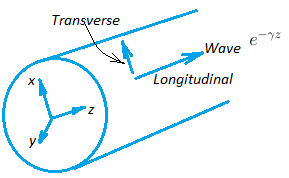
\includegraphics[width=0.7\linewidth]{./graphics/lect37}
\caption{An Arbitrarily Shaped Waveguide}
\label{fig:lect37}
\end{figure}
We can say this is a conducting pipe where the electromagnetic energy can flow along the axis of this pipe, there is wave propagation in the z-direction as shown. At the moment we are not even defining any shape for the cross-section, it could be rectangular, it could be circular or in general, it could be as arbitrarily shaped. The only information needed here is the direction of the wave, which is the z-direction. We develop a general framework starting from the Maxwell equations to show the kind of fields that exists inside the shape and then we will go on to deal with very specific cases of rectangular waveguides and propagation of modal propagation inside the rectangular waveguide. Any electric or magnetic field will be resolved into two components; one is along the wave propagation, called the longitudinal component and the other will be perpendicular to the direction of wave propagation called transverse.
\begin{equation*}
\bar{E} = \bar{E}_\bot + E_z\hat{z}
\end{equation*}
\begin{equation*}
\bar{H} = \bar{H}_\bot + H_z\hat{z}
\end{equation*}
\begin{equation*}
\bar{E}_\bot = E_x\hat{x} + E_y\hat{y}
\end{equation*}
\begin{equation*}
\bar{H}_\bot = H_x\hat{x} + + H_y\hat{y}
\end{equation*}
we define
\begin{equation}
\nabla = \nabla_\bot + \frac{\partial}{\partial z}\hat{z}
\label{eqn:transversegrad}
\end{equation}
where
\begin{equation*}
\nabla_\bot = \frac{\partial}{\partial x}\hat{x} + \frac{\partial}{\partial y}\hat{y}
\end{equation*}
Substituting equation~\ref{eqn:transversegrad} into Maxwell's equations\index{maxwell's equations} for the electric field;
\begin{align*}
\nabla\times\bar{E} = j\omega\mu\bar{H}
\end{align*}
\begin{dmath*}
\left[\nabla_\bot + \frac{\partial}{\partial z}\hat{z}\right]\times(\bar{E}_\bot + E_z\hat{z}) = -j\omega\mu(\bar{H}_\bot + H_z\hat{z})
\end{dmath*}
\begin{dmath*}
\nabla_\bot\times\bar{E}_\bot + \nabla_\bot\times(E_z\hat{z}) + \frac{\partial}{\partial z}\hat{z}\times\bar{E}_\bot + \frac{\partial}{\partial z}\hat{z}\times(E_z\hat{z}) = -j\omega\mu(\bar{H}_\bot + H_z\hat{z})
\end{dmath*}
Taking the transverse and longitudinal components and equating them on two sides
\begin{dmath*}
-j\omega\mu\bar{H}_\bot = \nabla_\bot\times(E_z\hat{z}) + \frac{\partial}{\partial z}\hat{z}\times\bar{E}_\bot
\end{dmath*}
\begin{dmath}
\bar{H}_\bot = -\frac{1}{j\omega\mu} \left[\nabla_\bot\times(E_z\hat{z}) + \frac{\partial}{\partial z}\hat{z}\times\bar{E}_\bot\right]
\label{eqn:transversemag}
\end{dmath}
Similarly, substituting equation~\ref{eqn:transversegrad}  into Maxwell's equation for the magnetic field;
\begin{align*}
\nabla\times\bar{H} = j\omega\epsilon\bar{E}
\end{align*}
\begin{dmath*}
\left[ \nabla_\bot + \frac{\partial}{\partial z}\hat{z} \right] \times (H_\bot + H_z \hat{z}) = \jmath \omega\epsilon (E_\bot + E_z \hat{z})
\end{dmath*}
\begin{dmath*}
\nabla_\bot\times H_\bot + \nabla_\bot\times H_z \hat{z} +  \frac{\partial}{\partial z}\hat{z}\times H_\bot + \frac{\partial}{\partial z}\hat{z}\times H_z \hat{z} = \jmath \omega\epsilon (E_\bot + E_z \hat{z})
\end{dmath*}
Taking the transverse and longitudinal components and equating them on two sides
\begin{dmath}
\bar{E}_\bot = \frac{1}{j\omega\epsilon} \left[\nabla_\bot\times H_z\hat{z} + \frac{\partial}{\partial z}\hat{z}\times\bar{H}_\bot\right]
\label{eqn:transverseele}
\end{dmath}
Substituting equation~\ref{eqn:transversemag} into \ref{eqn:transverseele}
\begin{dmath*}
\bar{E}_\bot = \frac{1}{j\omega\epsilon} \left[\nabla_\bot\times H_z\hat{z} + \frac{\partial}{\partial z}\hat{z}\times \left( -\frac{1}{j\omega\mu} \left[\nabla_\bot\times(E_z\hat{z}) + \frac{\partial}{\partial z}\hat{z}\times\bar{E}_\bot\right] \right)\right] 
\end{dmath*}
Collecting like terms
\begin{dmath}
\omega^2\mu\epsilon\bar{E}_\bot-\frac{\partial}{\partial z}\hat{z}\times\frac{\partial}{\partial z}\hat{z}\times\bar{E}_\bot = \frac{1}{j\omega\epsilon} \left[\nabla_\bot\times H_z\hat{z} - \frac{1}{j\omega\mu}\frac{\partial}{\partial z}\hat{z}\times\nabla_\bot\times E_z \hat{z} \right]
\label{eqn:electricfieldinwg}
\end{dmath}
Identity for vector triple product\index{vector triple product}
\begin{align*}
A\times B\times C = (\bar{A}\cdot\bar{C})\bar{B} - (\bar{A}\cdot\bar{B})\bar{C}
\end{align*}
\begin{dmath*}
\frac{\partial}{\partial z}\hat{z}\times\frac{\partial}{\partial z}\hat{z}\times\bar{E}_\bot = \frac{\partial}{\partial z}\hat{z}\left(\frac{\partial}{\partial z}\hat{z}\cdot\bar{E}_\bot\right)\hat{z} - \left(\frac{\partial}{\partial z}\hat{z}\cdot\frac{\partial}{\partial z}\hat{z}\right)\bar{E}_\bot = -\frac{\partial^2}{\partial z^2}\bar{E}_\bot
\end{dmath*}
where $\dfrac{\partial}{\partial z}\hat{z}\left(\dfrac{\partial}{\partial z}\hat{z}\cdot\bar{E}_\bot\right)\hat{z} = 0$
\begin{dmath*}
\frac{\partial}{\partial z}\hat{z}\times\nabla_\bot\times E_z\hat{z} = \nabla_\bot\left(\frac{\partial}{\partial z}\hat{z}.E_z\hat{z}\right) - \left(\frac{\partial}{\partial z}\hat{z}\cdot\nabla_\bot\right)E_z\hat{z} = \nabla_\bot\left(\frac{\partial E_z}{\partial z}\right)
\end{dmath*}
where $\dfrac{\partial}{\partial z}\hat{z}\cdot\nabla_\bot E_z\hat{z} = 0$. Substituting in equation~\ref{eqn:electricfieldinwg};
\begin{dmath}
\left[\omega^2\mu\epsilon\bar{E}_\bot+\frac{\partial^2}{\partial z^2}\bar{E}_\bot\right] = -j\omega\mu\nabla_\bot\times H_z\hat{z} + \nabla_\bot\left(\frac{\partial E_z}{\partial z}\right)
\end{dmath}
We have just taken two Maxwell equations, applied some vector identities, and derived the expressions for the transverse component of the electric field in terms of the longitudinal components. We did that because the waveguide is a structure in which the wave is going to propagate in the z-direction, this is the special direction in which ultimately the energy is going to flow.

Since this direction is the special direction in which the wave is propagating, generally we take the electric and magnetic field components which are in the z-direction that is the longitudinal component as independent components and try to express the transverse fields in terms of the longitudinal components and precisely that is what we did. We now got the expression for the transverse field in terms of the longitudinal component which is $E_z$ and z.

Since our problem again is the wave of propagation in the z-direction, we are assuming the wave is travelling in the z-direction. That means the travelling wave behaviour as we have seen earlier can be given as $e^{-\gamma z}$, where $\gamma$ is the propagation constant in the z-direction. So, the wave travels in the z-direction with a propagation constant $\gamma$. So, since we are now interested in the travelling wave inside the structure, we assume that the functional form of any field electric or magnetic in the z direction will be given $e^{-\gamma z}$

For a travelling wave in the z-direction;
\begin{align*}
\bar{E}, \bar{H} \sim e^{-\gamma z}\\
\frac{\partial}{\partial z} \equiv -\gamma\\
\frac{\partial^2}{\partial z^2} \equiv \gamma^2
\end{align*}
\begin{align*}
(\omega^2\mu\epsilon + \gamma^2)\bar{E}_\bot = -j\omega\mu\nabla_\bot\times(H_z\hat{z})-\gamma\nabla_\bot E_z
\end{align*}
Let's define
\begin{align}
\omega^2\mu\epsilon + \gamma^2 \equiv h^2
\label{eqn:h}
\end{align}
we will assign some physical meaning to h later. Therefore, the transverse components of electric and magnetic fields become
\begin{align}
\bar{E}_\bot = \frac{-j\omega\mu}{h^2}\nabla_\bot\times(H_z\hat{z}) - \frac{\gamma}{h^2}\nabla_\bot E_z
\label{eqn:transverseele2}
\end{align}
\begin{align}
\bar{H}_\bot = \frac{j\omega\epsilon}{h^2}\nabla_\bot\times(E_z\hat{z}) - \frac{\gamma}{h^2}\nabla_\bot H_z
\label{eqn:transversemag2}
\end{align}
$\nabla_\bot\times(H_z\hat{z})$ is representing a curl in the transverse plane, whereas $\nabla_\bot E_z$ is representing the gradient of this quantity $E_z$ which is the scalar quantity in the transverse plane. If we can solve the problem of wave propagation in terms of $E_z$ and $H_z$, then we can find out the corresponding fields in the transverse plane which are $\bar{E}_\bot$ and $\bar{H}_\bot$.

The approach for solving the problem, in general, will be as follows; We take a geometry in which we want to study the wave of propagation, find the solution for $E_z$ and $H_z$ for that geometry, then substitute into $\bar{E}_\bot$ and $\bar{H}_\bot$ expressions and then you get the component of transverse fields that is $E_x\ E_y\ H_x\ and\ H_y$.\\looking at $\bar{E}_\bot$ and $\bar{H}_\bot$ expressions, we can make certain conclusions. Firstly, if you assume that this medium is completely lossless, then this quantity $\gamma$ which is the propagation constant is purely imaginary because the wave is travelling and its amplitude is not going to change. For a lossless medium, we know that $\gamma$ should be $j\bar{\beta}$.
\section{Loss-less waveguide}
\begin{equation*}
\gamma = j\bar{\beta}
\end{equation*}
\begin{equation*}
\omega^2\mu\epsilon - \bar{\beta}^2 = h^2
\end{equation*}
If you recall $\omega^2\mu\epsilon$ or the phase constant of the wave in that unbound medium you find this quantity $h$ is nothing but the propagation constant of this wave in the transverse plane. $h$ represents the propagation constant of a wave in the transverse plane means in the XY-plane. From this expression now, few conclusions can be drawn. Firstly, if the transverse fields have to exist, then both $E_z$ and $H_z$ need not be zero but non-zero. Even if any one of them is non-zero, we can still get the transverse fields. That means we can have the field distribution inside this waveguide with either $E_z$ equal to 0 or $H_z$ equal to 0 or both of them non-zero.

However, if both of them are 0, then the transverse fields do not exist in general except when $h$ is equal to 0. So, now we have some interesting conclusions that can be drawn from this result that is for fields to survive inside the structure, both $E_z$ and $H_z$ cannot be 0 except in the case when x is equal to 0.
\begin{enumerate}[(i)]
\item Both $E_z$ and $H_z$ can not be 0 except when $h=0$.
\item When $h=0$, $E_z$ and $H_z$ MUST be zero.
\end{enumerate}

\paragraph{Case 1}When $E_z$ = 0, $H_z \neq 0 \Rightarrow TE$
\paragraph{Case 2}When $E_z \neq 0, H_z = 0 \Rightarrow TM$\\

The third configuration which is when $E_z$ is equal to 0 and $H_z$ is equal to 0, will give me the field, transverse fields provided when $h$ is equal to 0. But when $E_z$ and $H_z$ both are 0 that means we are talking about now the fields which are transverse electric and transverse magnetic fields. That means these field distributions must be the same as the transverse electromagnetic field.
So, what we conclude is very important and very profound which is that when $E_z$ and $H_z$ both are 0 which represents the transverse electromagnetic wave, for this wave, $h$ must be identically 0. So third case, when $E_z$ and $H_z$ both are 0, we get a wave which is transverse electromagnetic, TEM and for this, $h$ has to be 0.
\paragraph{Case 3}When $E_z = H_z = 0 \Rightarrow TEM$. For this $h \equiv 0$
\begin{dmath*}
\bar{\beta} = \sqrt{\omega^2\mu\epsilon - h^2}
\end{dmath*}
So, the conclusion that we draw here is whether we take a transverse electric case or transverse magnetic phase since in this case, $h$ cannot be 0 because otherwise, the transverse field will go to infinity, and it will become infinite, as it goes to 0. So, when any of these  $E_z$ and $H_z$ are not 0, $H$ cannot be 0 which means $H$ is always a finite quantity or the velocity proportional to related to this means the phase velocity will be a function of frequency. Whereas, if I take $h$ is equal to 0, then $\bar{\beta}$ will be $\omega \sqrt{\mu\epsilon}$ and the phase velocity will become independent of frequency. What that means is that TE mode or TM mode has to be always dispersive. The velocity will be a function of frequency, whereas the TEM mode has to be essentially non-dispersive because for this, now the phase velocity is going to be the velocity in that medium. We draw very important conclusions from here and these are;
\begin{enumerate}[(i)]
\item TE and TM modes are dispersive
\item TEM mode is non-dispersive
\end{enumerate}
That means whenever we try to excite the field distribution, they will be either transverse electric or transverse magnetic, and then we will always have their velocity varying the function of frequency. Whereas when we take a mode if at all it exists and if the mode is transverse electromagnetic, then this mode will always travel with a velocity independent of the frequency.

It is possible that for every structure you may not get the transverse electromagnetic mode propagating. But what we are saying is if at all the transverse electromagnetic modes exist on the structure, then this mode will be non-dispersive and it will be travelling with a speed which will always be the speed in the unbound medium which is spelling that waveguide. So, by doing this general analysis, we reached these very performed conclusions and now using this expression which you have derived, now we can analyze a particular waveguide propagation. Before we take up the specific problem, however, let us write down these quantities very explicitly which is
\begin{dmath*}
\nabla_\bot\times(\psi\hat{z}) \equiv 
\begin{vmatrix}
\hat{x} & \hat{y} &\hat{z}\\
\frac{\partial}{\partial x} & \frac{\partial}{\partial y} & o\\
0 & 0 & \psi
\end{vmatrix} = \frac{\partial\psi}{\partial y}\hat{x} - \frac{\partial\psi}{\partial x}\hat{y}
\end{dmath*}
In Cartesian coordinates, then we can use this expression to get a transverse field component in terms of the longitudinal components. Substituting this transverse gradient into equations \ref{eqn:transverseele2} and \ref{eqn:transversemag2} and simplifying, then the expressions essentially would look like
\begin{align}
E_x = -\frac{j\omega\mu}{h^2}.\frac{\partial H_z}{\partial y} - \frac{j\beta}{h^2}.\frac{\partial E_z}{\partial x}
\label{eqn:transverseex}\\
E_y = \frac{j\omega\mu}{h^2}.\frac{\partial H_z}{\partial x} - \frac{j\beta}{h^2}.\frac{\partial E_z}{\partial y}
\label{eqn:transverseey}\\
H_x = \frac{j\omega\epsilon}{h^2}.\frac{\partial E_z}{\partial y} - \frac{j\beta}{h^2}.\frac{\partial H_z}{\partial x}
\label{eqn:transversehx}\\
H_y = -\frac{j\omega\epsilon}{h^2}.\frac{\partial E_z}{\partial x} - \frac{j\beta}{h^2}.\frac{\partial H_z}{\partial y}
\label{eqn:transversehy}
\end{align}
The expressions are quite symmetric in that sense and they are very easy to remember also. So with this, now development, general development for the propagation of a mode inside a waveguide; now we are prepared to take very specific cases and as we saw that there are two types of modes which can exist, the transverse electric mode and the transverse magnetic mode, we also saw a special case which for the transverse electromagnetic mode and now we take a very specific case that is what is called a rectangular waveguide. That is if the cross-section of this pipe which we talked about is rectangular; then what kind of fields are going to propagate inside this waveguide?
% \chapter{Rectangular Waveguide (1)}
In the previous chapter, we developed a general approach for analysing wave propagation inside a waveguide. In this chapter, we will consider a waveguide whose cross section is rectangular. This is called a \textbf{Rectangular Waveguide}\index{rectangular waveguide}. This rectangular pipe is assumed to be made of ideal conductor $\sigma = 0$ and the medium filling this waveguide is an ideal dielectric $\sigma = 0$. We are concerned with the propagation and derivation of these parallel waves in a rectangular waveguide referred to as TE and TM modes, using the same general approach in waveguide analysis.

The waveguide in figure~\ref{fig:lec38fig1} shows the x, y and z coordinates in which the electromagnetic wave is propagated. It is propagated along the z direction. $a$ is the width of the guide while the $b$ is the breadth of the guide. In this guide $a \geq b$.

\begin{figure}[h]
\centering
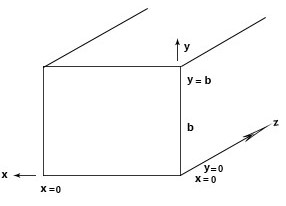
\includegraphics[width=0.7\linewidth]{./graphics/lec38fig1}
\caption{A Rectangular Waveguide}
\label{fig:lec38fig1}
\end{figure}

\section{Transverse Magnetic ($TM$) mode}\index{transverse magnetic mode}
Considering the transverse magnetic (TM mode), $ E_{z} = 0$, $H_{z} = 0 $ longitudinal components. For a transverse field to exist, either $ E_{z} $ or $ H_{z} $ has to be zero. $ H_{z} $ is oriented on the transverse plane and $ E_{z} $ on the longitudinal plane.

Now we first find the solution of the longitudinal component $ E_{z} $ and then find the transverse component $ H_{z} $, and then we apply an initial condition to it. We can use the equations~\ref{eqn:transverseex}-\ref{eqn:transversehy} derived for the TE and TM modes, rewritten as:
\begin{align}
E_x = -\frac{j\omega\mu}{h^2}.\frac{\partial H_z}{\partial y} - \frac{j\beta}{h^2}.\frac{\partial E_z}{\partial x}
\label{eqn:transverseex2}\\
E_y = \frac{j\omega\mu}{h^2}.\frac{\partial H_z}{\partial x} - \frac{j\beta}{h^2}.\frac{\partial E_z}{\partial y}
\label{eqn:transverseey2}\\
H_x = \frac{j\omega\epsilon}{h^2}.\frac{\partial E_z}{\partial y} - \frac{j\beta}{h^2}.\frac{\partial H_z}{\partial x}
\label{eqn:transversehx2}\\
H_y = -\frac{j\omega\epsilon}{h^2}.\frac{\partial E_z}{\partial x} - \frac{j\beta}{h^2}.\frac{\partial H_z}{\partial y}
\label{eqn:transversehy2}
\end{align}
$ \omega $  is the frequency of the wave, $ \mu $   is the permeability of the medium, $ \epsilon $ is the permittivity of the medium filling the waveguide. We expand $ \nabla^{2} $ in the cartesian coordinate system.
\begin{equation}
\frac{\partial ^{2} E_z}{\partial x^2} + \frac{\partial ^2 E_z}{\partial y^2} + \frac{\partial ^2 E_z}{\partial z^2}+ \omega^2\mu\epsilon {E_{z}} = 0
\label{eqn:maxwellele}
\end{equation}

%\begin{figure}
%\centering
%\includegraphics[width=0.7\linewidth]{./graphics/lec38fig2}
%\caption{wave propagation along z}
%\label{fig:lec38fig2}
%\end{figure}
So whatever solution we are going to get for this problem, must have a standing wave kind solution in the x direction with $b\rightarrow \infty$, the same is true if $a\rightarrow \infty$, the standing wave will be in the y direction. Hence, the solution along the x and y directions must be of standing wave type. The solution along the z direction must be of the travelling wave type in the direction of the wave propagation. With this understanding, now we solve the problem. With
\begin{equation}
E_z (x,y,z) = X(x)Y(y)Z(z)
\label{eqn:electricwave}
\end{equation}
Substitute equation~\ref{eqn:electricwave} into equation~\ref{eqn:maxwellele}
\begin{align}
YZ \dv[2]{X}{x} + XZ \dv[2]{Y}{y} + XY \dv[2]{Z}{z}+ \omega^2\mu\epsilon {XYZ} = 0
\end{align}
The partial derivatives have been converted to full ones since $X$, $Y$, and $Z$ are only functions of $x$, $y$, and $z$. Dividing through the expression by $XYZ$ gives
\begin{align}
\frac{1}{X}\dv[2] {X}{x} + \frac{1}{Y}\dv[2]{Y}{y} + \frac{1}{Z} \dv[2]{Z}{z} + \omega^2\mu\epsilon = 0
\label{eqn:diffeqn}
\end{align}
From the equation, $\frac{1}{X}\dv[2] {X}{x}$ is only a function of $x$, $\frac{1}{Y}\dv[2]{Y}{y}$ is only a function of $y$ and $\frac{1}{Z} \dv[2]{Z}{z}$ is only a function of $z$. So this equation that we have written is a \textbf{Point relation}\index{point relation} that should be valid at every point in space. The equation must be satisfied by every point ($x$, $y$, $z$) in the 3D space. That can only happen if $\frac{1}{X}\dv[2] {X}{x}$, $\frac{1}{Y}\dv[2]{Y}{y}$, and $\frac{1}{Z} \dv[2]{Z}{z}$ are constant quantities.

Let,  
\begin{align*}
\frac{1}{X}\dv[2]{X}{x} = -A^2\\
\frac{1}{Y}\dv[2]{Y}{2} = -B^2\\
\frac{1}{Z}\dv[2]{Z}{z} = -\beta^2
\end{align*}
$-A^2$, $-B^2$ and $-\beta^2$ are chosen in such a way that we can always have a standing wave kind of solution in $x$ and $y$ directions while we have a travelling wave solution in the $z$ direction. $\beta$ is the phase constant of the mode of propagation. Thus we have second homogeneous equations as follows:
\begin{align*}
\dv[2]{X}{x} + A^2X = 0\\
\dv[2]{Y}{y} + B^2Y = 0\\
\dv[2]{Z}{z} + \beta^2Z = 0
\end{align*}
Whose solution becomes,   
\begin{align*}
X(x) = C_{1}\cos Ax + C_{2}\sin Ax\\
Y(x) = C_{3}\cos By + C_{4}\sin By\\
Z(x) = C_{5} e^{-j \beta z} + C_{6} e^{+j \beta z}
\end{align*}                                  
The cosine and sine functions show amplitude variation which is a standing wave kind of behaviour. The $C_{5}e^{+j\beta z}$ and $C_{6}e^{-j\beta z}$ are travelling waves in the positive and negative z-direction respectively which indicates the forward and backward travelling waves. So when writing the solution we use our understanding that we have developed from the parallel plane waveguide. That is in the transverse direction, between the two conducting boundaries, we must have a solution that is like a standing wave kind of solution. Along the length of the pipe in which the energy is being propagated, we have a travelling wave kind of solution.

Our solution shows that there are two waves on the structure travelling in the positive and negative z directions. However, if we assume that this waveguide is of infinite $\infty$ distance in the z direction, then there is no reflection. As we have seen from the transmission line, there is no reflection if the transmission line is infinite. So for simplicity of the analysis we assume, there is no wave travelling in the negative z direction and that we have only the forward wave.

Therefore, by substituting the above equations into equation~\ref{eqn:electricwave} we can then write the general equation for the component $E_{z}$. However, for no backward wave, $C_6 = 0$  so that $Z(z) = C_5e^{-\jmath\beta z}$. Thus the general solution for the wave equation $E_z = XYZ$ is
\begin{equation*}
E_{z} = C_{5}(C_{1}cos Ax + C_{2}sin Ax)(C_{3}\cos By + C_{4}sin By) e^{-j\beta z}
\end{equation*}
Now we apply the boundary condition on $E_{z}$ to obtain the constants.  In this case, we are having $E_z$ being tangential to the four walls that make up the waveguide. Hence, we would have four boundary conditions, one for each wall at
\begin{enumerate}[(i)]
\item x = 0
\item x = a 
\item y = 0
\item y = b
\end{enumerate}   
At these four walls, tangential components of electric fields should be zero, i.e. $E_z = 0$ at $x=0$, $x=a$, $y=0$ and $y=b$. At $x=0$,  
\begin{dmath*}
E_{z} = C_{5}(C_1 + 0)(C_3\cos By + C_4\sin By)e^{-\jmath\beta z} = 0
\end{dmath*}
or
\begin{align*}
C_1 C_{5}(C_3\cos By + C_4\sin By)e^{-\jmath\beta z} = 0\\
\longrightarrow C_1 = 0
\end{align*}
$C_1 = 0$ will make $E_z = 0$ for $x=0$ term. At $y=0$,
\begin{dmath*}
E_{z} = C_{5}(C_1 \cos Ax + C_2\sin Ax)(C_3 + 0)e^{-\jmath\beta z} = 0
\end{dmath*}
$C_3 = 0$ will make $E_z = 0$ for $y=0$ so we have reduced $E_z$ to
\begin{dmath*}
E_{z} = C_{5}C_{2}\sin AxC_{4}\sin By e^{-j\beta z} = C_5C_4C_2\sin Ax\sin By e^{-j\beta z}
\end{dmath*}
Let C = $ C_{5}C_{2}C_{4} $
\begin{equation}
E_{z} = C\sin Ax\sin By e^{-j\beta z}
\label{eqn:elesoln}
\end{equation}
Equation~\ref{eqn:elesoln} satisfies the boundary condition $E_z = 0$ at $x=0$ and $y=0$. If $E_z = 0$ at $x=a$ and $y=b$ then
\begin{equation*}
Aa = m\pi,\ A = \frac{m\pi}{a}\footnote{This happens when $\sin Aa = 0$ or $Aa = m\pi$}
\end{equation*}
\begin{equation*}
Bb = n\pi,\ B = \frac{n\pi}{b}\footnote{This happens when $\sin Bb = 0$ or $Bb = n\pi$}
\end{equation*}
$m$ and $n$ are integers. Thus, substituting $A$ and $B$ into equation~\ref{eqn:elesoln}.
\begin{dmath}
E_{z} = C sin\frac{m\pi x}{a} sin\frac{n\pi y}{b} e^{-j\beta z}
\label{eqn:elesoln2}
\end{dmath}
Equation~\ref{eqn:elesoln2} satisfies all four boundary conditions and is the general solution of the wave equation for a rectangular waveguide. $C$ represent the amplitude of the electric field and has nothing to do with the boundary conditions. Since boundary conditions are satisfied irrespective of the power level or the amplitude of the field, $C$ will remain as it is. When we talk about the power inside the mode, only then will the constant $C$ be evaluated. The two quantities $m$ and $n$ now represent the order of the mode, by the same token as what we have done for the parallel plane waveguide when we had a mode and put an index. Now we put two indices for $m$ and $n$. So a transverse magnitude mode can now be designated by $TM_{mn}$ and $m$ is the index around in the broader dimension, $a$, and the $n$ is the index around the shorter dimension, $b$. So the first index tells the field variations along the broader dimension of the waveguide, which is the x direction and the second index tells the field variations along the shorter dimension of the waveguide. 

If $m=1$, from 0 to a, we have one half-cycle variation. If $m=2$, we have two half-cycle variations and so on. Hence this behaviour is essentially identical to what we have seen for the parallel plane waveguide in that the order or index which we have in the mode represents the number of half-cycles in the transverse direction. $m$ in this case are two transverse directions, one in x and another in y. So along x and y, $m$ and $n$ represent the number of half-cycle variations for the field. 

In equation~\ref{eqn:elesoln2}, suppose $a$ or $b$ tends to infinity, it becomes a parallel plane waveguide and then the equation which has for $E_z$ by satisfying either $a=\infty$ or $b=\infty$. Now that we have the constants $m$ and $n$, there are a few things which should be noted. First, $m = 0$ and $n=0 \Rightarrow E_z = 0$. This means that $TM_{00}$ cannot get excited inside a rectangular waveguide.

For parallel plane waveguide, $TM_0$ mode which was the same as $TEM$ mode was possible and it was the \textbf{lowest order} mode. However, for this mode with $m=n=0$, $E_z$ goes to zero in the rectangular waveguide. So $TM_{00}$ does not exist. Also, we note that when any of the indexes go to zero, then $E_z$ goes to zero. $H_z$ is always zero for transverse magnetic mode, so with $E_z$ and $H_z$ going to zero, all fields (all depend on $E_z$ and $H_z$) will identically go to zero. 

\section{Dispersion Relation}
From equation~\ref{eqn:diffeqn} if we substitute the constants, then
\begin{dmath*}
-A^2 - B^2 - \beta + \omega^2\mu\epsilon = 0
\end{dmath*}
But $A=\dfrac{m\pi}{a}$ and $B=\dfrac{n\pi}{b}$ so,
\begin{align}
-\left(\frac{m\pi}{a}\right) - \left(\frac{n\pi}{b}\right) - \beta^{2} + {\omega^2\mu\epsilon} = 0
\label{eqn:hrec}
\end{align}
\begin{equation}
\beta = \sqrt{{\omega^2\mu\epsilon} - \frac{m\pi}{a} - \frac{n\pi}{a}}
\label{eqn:dispersionrelatn}
\end{equation}
This equation is similar to that of the parallel plane waveguide $\bar{\beta} = \sqrt{\omega^2\mu\epsilon - \left(\dfrac{m\pi}{a}\right)}$ where $a=d$ the height of the waveguide. Hence equation~\ref{eqn:dispersionrelatn} tells how the velocity varies as a function of frequency.
\begin{dmath*}
v_p = \frac{\omega}{\beta} = \frac{\omega}{\sqrt{{\omega^2\mu\epsilon} - \frac{m\pi}{a} - \frac{n\pi}{a}}}
\end{dmath*}
Equation~\ref{eqn:dispersionrelatn} is called the \textbf{dispersion relation}\index{dispersion relation} for a transverse magnetic mode on a rectangular waveguide. So this is the dispersion relation for $TM_{mn}$ mode when either $m$ or $n$ is not zero. 

Comparing eqaution~\ref{eqn:hrec} with equation~\ref{eqn:h}.
\begin{dmath*}
h^{2} =  \frac{m\pi}{a} + \frac{n\pi}{b}
\end{dmath*} 
So when $m$ and $n$ are both non-zero, then $h^2$ is not zero. When $h^2$ is not zero, the field will have transverse fields represented in terms of longitudinal components $E_z$ and $H_z$. From the equations for the transverse fields in equations~\ref{eqn:transverseex2}-\ref{eqn:transversehy2} rewritten here,
\begin{align*}
E_x = -\frac{j\omega\mu}{h^2}.\frac{\partial H_z}{\partial y} - \frac{j\beta}{h^2}.\frac{\partial E_z}{\partial x}\\
E_y = \frac{j\omega\mu}{h^2}.\frac{\partial H_z}{\partial x} - \frac{j\beta}{h^2}.\frac{\partial E_z}{\partial y}\\
H_x = \frac{j\omega\epsilon}{h^2}.\frac{\partial E_z}{\partial y} - \frac{j\beta}{h^2}.\frac{\partial H_z}{\partial x}\\
H_y = -\frac{j\omega\epsilon}{h^2}.\frac{\partial E_z}{\partial x} - \frac{j\beta}{h^2}.\frac{\partial H_z}{\partial y}
\end{align*}
If both $E_z$ and $H_z$ are zero, and $h$ is non zero all transverse fields go to zero and so no transverse field exists. $h$ is non zero means $m$ and $n$ are non zero. Hence we can see that for a transverse magnetic mode when either $m$ or $n$ is zero, then $E_z=0$ and $h\neq 0$, the transverse fields will go to zero and the mode will not exist.

So we have important conclusions to derive as follows:
\begin{enumerate}[(i)]
\item $TM_{00}$ does not exist
\item $TM_{m0}$ and $TM_{0n}$ also do not exist
\item $TM_{11}$ is the lowest order of TM mode which can exist on the waveguide.
\end{enumerate}
So we conclude that if the $TM$ mode must be excited in the rectangular waveguide, the field must vary in the x and y direction along the rectangular waveguide. With $m=0$, no variation of fields along the x direction and no variation along the y axis when $n=0$. If $E_z \neq 0$, at $m=0$, $E_z=0$ at $x=0$ and at $x=a$. If there should be no variation, then $E_z$ has to be identically zero everywhere. This is true along the $y$ direction also. This makes sense physically as $E_z$ cannot exist without a variation in the x and y direction. We have also seen from the solution in the cartesian coordinates that the variation is always sinusoidal going in terms of the number of half cycles ($m$ and $n$) in the x or y direction. So the fields in the transverse direction always vary sinusoidally in the cartesian coordinate system. It must vary else the field cannot exist inside. These are the important conclusions which we can draw for the transverse magnetic mode.

Once we get $E_z$, we can substitute into equations for the transverse fields, equations~\ref{eqn:transverseex2}-\ref{eqn:transversehy2}, with $H_{z} = 0$ for $TM$.
\begin{dmath*}
E_x = -\frac{j \beta}{h^2}\cdot\pdv{E_{z}}{x} = -\frac{j \beta}{h^{2}}\cdot\left(\frac{m\pi}{a}\right) C\cos \left(\frac{m\pi x}{a}\right)\sin \left(\frac{n\pi y}{b}\right)e^{-j \beta z}
\end{dmath*}
\begin{dmath*}
E_y = -\frac{j \beta}{h^2}\cdot \pdv{E_z}{y} = -\frac{j \beta}{h^{2}}\left(\frac{n\pi}{b}\right) C \sin\left(\frac{m\pi x}{a}\right)\cos \left(\frac{n\pi y}{b}\right)e^{-j \beta z}
\end{dmath*}
\begin{dmath*}
H_x = \frac{j \omega\epsilon}{h^2}\cdot\pdv{E_z}{y} = \frac{j \omega\epsilon}{h^{2}}\cdot\left(\frac{n\pi}{a}\right) C \sin \left(\frac{m\pi x}{a}\right)\cos \left(\frac{n\pi y}{b}\right)e^{-j \beta z}
\end{dmath*}
\begin{dmath*}
H_y =-\frac{j \omega\epsilon}{h^2}\pdv{E_z}{x} = -\frac{j \omega\epsilon}{h^{2}}\left(\frac{m\pi}{b}\right) C \cos \left(\frac{m\pi x}{a}\right)\sin \left(\frac{n\pi y}{b}\right)e^{-j \beta z}
\end{dmath*}

Now we get the amplitude field for the $TM$ mode in a rectangular waveguide. With the understanding that the lowest order mode in the structure will be $TM_{11}$ mode. With $E_z = C\sin\left(\dfrac{m\pi x}{a}\right)\sin\left(\dfrac{n\pi y}{b}\right)e^{-\jmath\beta z}$, we see that $E_z = 0$ cross-section of the waveguide as shown in figure~\ref{fig:lec38fig3}, the variation of the field in the half-cycles is shown based on the different values of m and n.
\begin{figure}[h]
\centering
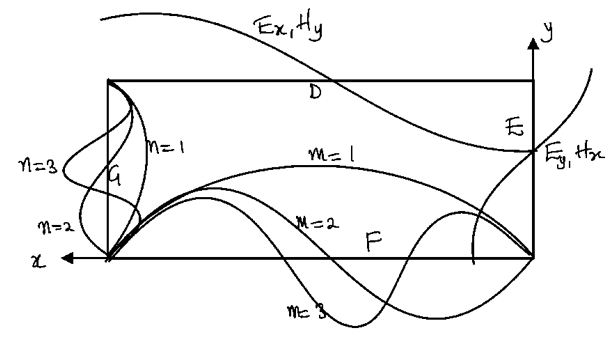
\includegraphics[width=0.7\linewidth]{./graphics/lec38fig3}
\caption{TM mode patterns}
\label{fig:lec38fig3}
\end{figure}
Comparing $E_x$ which we derived with 
\begin{dmath*}
E_x = K \times \cos\left(\frac{m\pi x}{a}\right)\sin\left(\frac{n\pi y}{b}\right)
\end{dmath*}
For $m=1$, $K\cos\left(\dfrac{\pi x}{a}\right)\sin\left(\dfrac{n\pi y}{b}\right)$. $x=0$ gives maximum, $x=a$ gives a negative minimum. So the field of $E_x$ with $m=1$ still has the half-cycle variation like $E_z$, but the maximum and minimum points differ from that of $E_z$. $E_y$ field has cosine variation along y with $m=1$ we have just half-cycle going in the form shown in figure~\ref{fig:lec38fig3}.

So components $E_x$ and $E_y$ will be staggered in space with respect to the $E_z$ component (longitudinal component). Once we have this understanding, we see that $E_x$ and $H_y$ have the same behaviour comparing their expressions. What we observe from here and from the rigorous analysis is that the cross-section of the waveguide shown in figure~\ref{fig:lec38fig3} as D, E, F, and G which are the sides of the waveguide are
\begin{enumerate}[(i)]
\item $H_y$ is tangential to sides E and G of the waveguide
\item $H_y$ is maximum and side E pointing in the position y direction reduces as you move away towards the left side of E. It goes to zero at $x=\dfrac{a}{2}$, changes direction and starts increasing in the opposite direction till it is maximum again at $x=a$ ( in the opposite direction to that at $x=0$). 
\end{enumerate}
This variation of $H_y$ is sinusoidal to make a certain number of half-cycles depending on the order of mode. Similarly 
\begin{enumerate}[(i)]
\item $H_x$ is tangential to sides D and F of the waveguide
\item $H_x$ at D is maximum and points in the position x direction; it reduces as you move upward to 0 at $y=\dfrac{b}{2}$ the middle point. Beyond this point, it changes direction till it gets to another maximum at F which is opposite it its original maximum at D. 
\end{enumerate}
The number of half-cycles depends on order n. Hence, this explanation is based on $n=1$. We looked at only the variations of $E_x$ along y, to have $E_x = K\sin\left(\dfrac{n\pi y}{b}\right)$. $E_x$  is also tangential to sides D and F of the waveguide. With $n=1$, $E_x = K\sin\left(\dfrac{\pi y}{b}\right)$. So at $H_x = $ maximum, say $y=0$, $E_x = 0$ because of sinusoidal variations. $H_x$ was a cosine variation at $Y=\dfrac{b}{2}$, $E_X = $ maximum, whereas $H_x = 0$ at that point.

Whatever magnetic field on the tangential surface is balanced by the surface current so that the boundary conditions of the tangential component of the magnetic field can hold. So the magnetic field is maximum on the conducting boundary and having understood that the solution gives a sinusoidal variation in the transverse direction. The same inference can be made for the \textbf{transverse electric} mode without going through the same analysis to derive the solution of the transverse fields.

\section{Transverse Electric mode ($TE$) mode}\index{transverse electric mode}
For the transverse electric mode, $E_{z} = 0$ and $H_{z}$, with $H$ always maximum on the boundary and $E$ minimum on the boundary, we can write the solution to the $TE$ mode without going through the rigorous analysis as we did in the $TM$ mode.
\begin{equation}
H_z = C\cos\left(\frac{m\pi x}{a}\right) \cos\left(\frac{n\pi y}{b}\right)e^{-j\beta z}
\label{eqn:wavesolnhz}
\end{equation}
This is the solution we would derive if we go through the same routine of finding the general solution for $H_z$, then finding out the transverse components of $H$ that are tangential to the boundary and then applying the boundary conditions on those components. It is important to note that the longitudinal components of magnetic fields $H_z$ do not have boundary conditions, so fo the $TE$ case if we go through the routine analysis, there will be two stops involved. First, finding the general solution of the $H_z$ from the wave equation and second, getting the transverse components $H_x$ and $H_y$ for which we apply the boundary conditions. \textbf{No boundary condition for} $\boldsymbol{H_z}$.

However, without going through the same analysis, we developed the understanding that the tangential component of the magnetic field to the conducting surface of the waveguide is maximum. Thus, we get the solution for $H_z$ as in equation~\ref{eqn:wavesolnhz}. Theses fields are maximum with $x=0$, $x=a$ and $y=0$ and $y=b$. So these fields have a variation which we are looking for, that those tangential components of the magnetic field must be maximum at the boundary surface. Using this expression for $H_z$. Now we could investigate the transverse electric mode and see the characteristics of $TE$ mode and then compare the behaviour of this mode with the $TM$ mode.
% \chapter{Rectangular Waveguide (2)}

We are investigating the propagation of electromagnetic waves inside a hollow pipe with a rectangular cross-section. We called this structure a rectangular waveguide. We had the structure for a rectangular waveguide shown below. With energy flowing along the length of the pipe. The coordinate axis is oriented in the direction shown with $a\geq b$.
\begin{figure}[h]
\centering
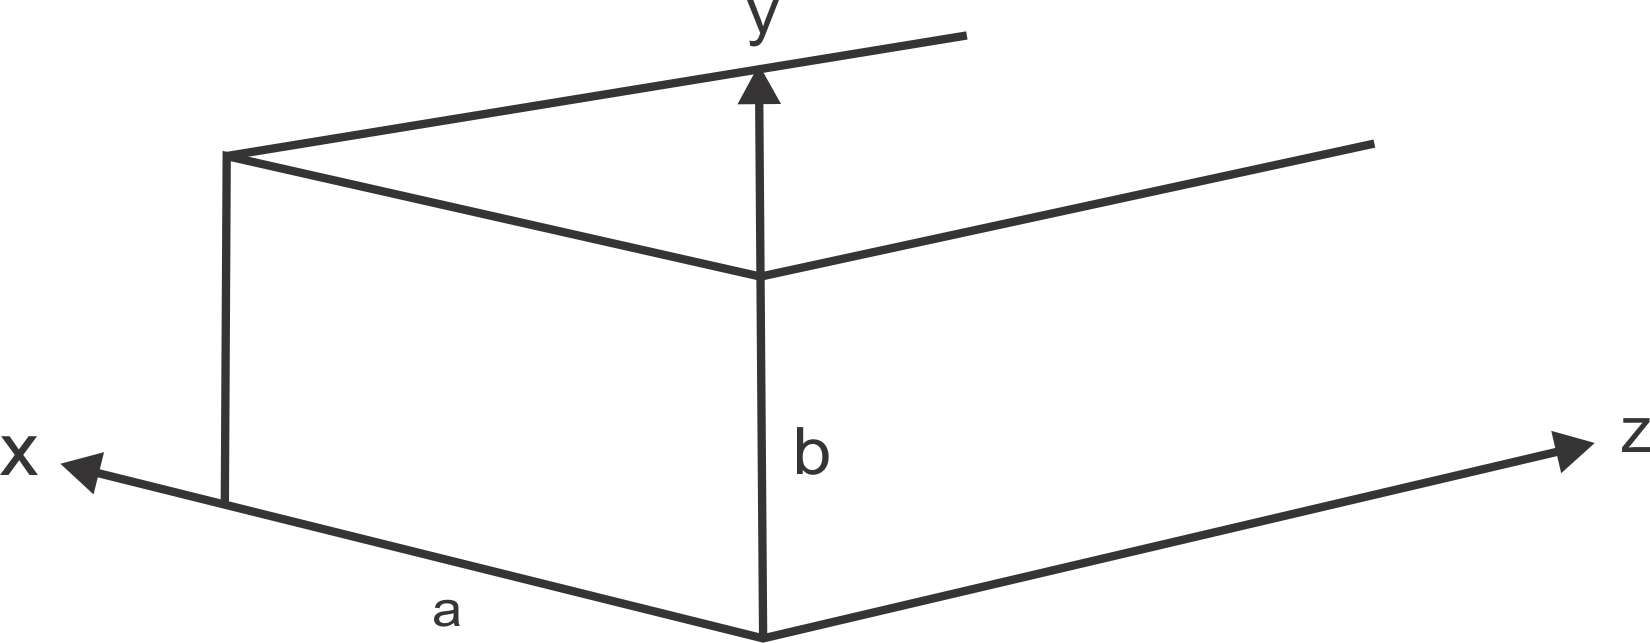
\includegraphics[width=1\linewidth]{./graphics/group39}
\caption{A rectangular waveguide with $a>b$}
\end{figure}

\section{Transverse Electric  ($TE$) mode}\index{transverse electric mode}
For the transverse electric mode, we had $E_z = 0$, $H_z \neq 0$ and by comparison we had 
\begin{dmath}
H_z = C\cos(\frac{m\pi x}{a}) \cos(\frac{n\pi y}{b})e^{-j\beta z}
\label{eqn:magneticfield}
\end{dmath}

Like the case of the transverse magnetic, we denote this by $TE_{mn}$ to show the order of the transverse electric mode. We ask what are indexes required for the existence of these fields. If $m = n = 0$ i.e $TE_{00},H_z$ is not zero unlike the $TM_{00}$ mode. Recall that the transverse fields from equations~\ref{eqn:transverseex}-\ref{eqn:transversehy} expressed as:
\begin{align*}
E_x = -\frac{j\omega u}{h^2}\frac{\partial H_z}{\partial y} - \dfrac{j\beta}{h^2}\frac{\partial E_z}{\partial x}\\
E_y = \frac{j\omega u}{h^2}\frac{\partial H_z}{\partial x} - \dfrac{j\beta}{h^2}\frac{\partial E_z}{\partial y}\\
H_x = \frac{j\omega \epsilon}{h^2}\frac{\partial E_z}{\partial y} - \dfrac{j\beta}{h^2}\frac{\partial H_x}{\partial x}\\
H_y = -\frac{j\omega \epsilon}{h^2}\frac{\partial E_z}{\partial x} - \dfrac{j\beta}{h^2}\frac{\partial H_z}{\partial y}
\end{align*}
All the transverse fields involve space derivation, $\dfrac{\partial}{\partial x}$ or $\dfrac{\partial}{\partial y}$. So having a field which does not vary as a function of space $(x,y)$ for $TE_{00}$, $H_z = Ce^{-j\beta z}$  $\dfrac{\partial H_z}{\partial x}$,  $\dfrac{\partial H_z}{\partial y} = 0$ and $E_z = 0$. So that $E_x, E_y, H_x$ and $H_y$ will all go to zero. So if $m = n = 0, H_z = C \Rightarrow E_\bot , H_\bot = 0$. This means that in this situation of $m = n = 0$ for TE, we have magnetic field $H_z = Ce^{-j\beta z}$ but no electric field. What we have seen for a time-varying field is such that this can't happen as electric and magnetic fields are coupled. So if the electric field goes to zero, then the magnetic field must go to zero. This means that the constant $C$ is $H_z = Ce^{-j\beta z}$ must be identically equal to zero. This means that mode $TE_{00}$ cannot exist like $TM_{00}$.

Let's consider $H_z$ from equation~\ref{eqn:magneticfield} when $m$ or $n = 0$,
\begin{dmath*}
H_z = C \cos \left(\frac{m\pi x}{a}\right)\cos\left(\frac{n\pi y}{b}\right)e^{-j\beta z} = C \cos \left(\frac{n\pi y}{b}\right)e^{-j\beta z} \neq 0 
\end{dmath*}
or 
\begin{dmath*}
H_z = C \cos \left(\frac{m\pi x}{a}\right)e^{-j\beta z} \neq 0 
\end{dmath*}
That means $TE_{0n}$ or $TE_{m0}$ does not exist. The $TE_{0n}$ meant that the field has variation in the y-direction and $TE_{m0}$ meant that the field has variation in the x-direction but no variation in the y-direction. Hence the lowest order modes for TE mode will be $TE_{10}$ or $TE_{01}$ compared to $TM_{11}$ in TM mode. 

\section{Phase Constant}\index{phase constant}
Using a similar analysis to the TM mode, it can be shown that 
$$h^2 =\left(\dfrac{m\pi}{a}\right)^2 + \left(\dfrac{n\pi}{b}\right)^2$$ 
and then we get phase constant in the z-direction as 
$$\beta = \sqrt{\omega^2\mu\epsilon-\left(\dfrac{m\pi}{a}\right)^2- \left(\dfrac{n\pi}{b}\right)^2}$$
$\bar{E},\bar{H}\sim e^{-j\beta z}$ i.e $\bar{E}\ and\ \bar{H}$ has a variation with $e^{-j\beta z}$. To show the travelling $\omega^2\mu\epsilon < \left[\left(\dfrac{m\pi}{a}\right)^2 + \left(\dfrac{n\pi}{b}\right)^2\right]$, then the phase constant becomes imaginary. At this point $e^{-j\beta z}$ does not represent a travelling wave, but exponentially decaying fields in the z-direction and the wave propagation cases.

Hence we see that the frequency must have certain values so that $\beta$ is a real quantity. That frequency as we saw in a parallel plane waveguide where the transition takes place from wave to decaying field is the cut-off frequency of the mode. So far different values of $m$ and $n$ will have different cut-off frequencies. 

\section{Cut-off Frequencies}
At cut-off frequency ${\omega_c}^2\mu\epsilon = \left(\dfrac{m\pi}{a}\right)^2 + \left(\dfrac{n\pi}{b}\right)^2$
\begin{dmath}
f_c = \frac{1}{2\pi \sqrt{\mu\epsilon}}\left[\left(\frac{m\pi}{a}\right)^2 + \left(\dfrac{n\pi}{b}\right)^2\right]^{\frac{1}{2}}
\label{eqn:cut-off}
\end{dmath}
Now knowing the order $m$ and $n$, and the dimension of the waveguide, we can determine the cut-off frequency for a particular mode.
\begin{dmath*}
\beta = \sqrt{{\omega}^2\mu\epsilon-{\omega_c}^2\mu\epsilon}
\end{dmath*}
since ${\omega_c}^2\mu\epsilon = \left(\dfrac{m\pi}{a}\right)^2 + \left(\dfrac{n\pi}{b}\right)^2$
\begin{dmath*}
\beta =\omega\sqrt{\mu\epsilon}\left[1-{\frac{\omega c}{\omega}}\right]^{\frac{1}{2}} = \frac{\omega}{c}\left [1-{\frac{fc}{f}}\right]^{\frac{1}{2}} \frac{1}{\sqrt{\mu\epsilon}}= c
\end{dmath*}
so $\omega{\sqrt{\mu\epsilon}}= \dfrac{\omega}{c}$
\begin{dmath}
\beta = \frac{2\pi f}{c}\left[1-\left(\frac{f_c}{f}\right)^2\right]
= \frac{2\pi}{\lambda}\left[1-\left(\frac{f_c}{f}\right)^{\frac{1}{2}}\right]
\label{eqn:phaseconstrec}
\end{dmath}
Now, this is the phase constant for the waveguide in the z-direction. Now we imagine we have this structure for which the quantity we had to measure was the variation of the electric field along the length, say we take a probe to measure the field along the length, you will observe a separation distance between two consecutive maxima that is related to the phase constant of the wave along the direction of the waveguide $\dfrac{2\pi}{\lambda}$ is what we will measure in this waveguide. This $\lambda$ is what the wave has intrinsically in an unbound medium.

For our case, let's say $\beta = \dfrac{2\pi}{\lambda}$, $\lambda$ is not the wavelength in unbound medium $\frac{c}{f}$, so we are better off saying  $\beta = \dfrac{2\pi}{\lambda_g}$. ${\lambda_g}$ best describes the distance between two maxima of the electric field that we would measure inside the rectangular waveguide. So $\lambda$ is the intrinsic wavelength\index{intrinsic wavelength} of the wave in an unbound medium $\dfrac{c}{f}$, inside the wavelength we have a modified wavelength to $\lambda_g$ which is related to $\lambda$. So $\lambda g$ is the wavelength for the guided electric and magnetic field distribution inside the rectangular waveguide and it is called the \textbf{Guided Wavelength}\index{guided wavelength}. 

\section{Guided Wavelength}
$\beta$ is the phase constant we measured as we move the probe along to get successive maxima inside the waveguide.$\lambda$ is not what we measure along the waveguide but $\lambda_g$

From equation~\ref{eqn:phaseconstrec}, $\beta$ is related to  $\beta = \dfrac{2\pi}{\lambda_g}$, then 
\begin{dmath}
\lambda_g = \frac{\lambda}{\left[1-{\frac{fc}{f}}\right]^{\frac{1}{2}}}
\label{eqn:lambdag}
\end{dmath}
where $\lambda$ is the wavelength of the wave in unbound medium $\lambda_g$ is the wavelength which we will measure inside the bound structure along the waveguide. For travelling wave $f>f_c$ otherwise $\lambda$ is a complex number that results in exponentially decaying fields. So $\left[1-{\dfrac{fc}{f}}\right]^{\frac{1}{2}}$ is always going to be less than 1. This means $\lambda_g>\lambda$. Hence guided wavelength is always greater than the intrinsic wavelength of the medium. As $f\longrightarrow0$, $\dfrac{f_c}{f}\longrightarrow0$ at that time, $\lambda_g\longrightarrow\lambda$ but never become $\lambda$ because we would always have a finite frequency. So for a guided structure, no matter what frequency we operate at $\lambda_g>\lambda$.

Secondly, as $f\longrightarrow f_c$, when $f=f_c$, $\lambda_g = \dfrac{\lambda}{0} = \infty$ so $\lambda_g\longrightarrow\infty$ when $f\longrightarrow f_c$. We know that phase velocity $V_\rho = \dfrac{\omega}{\beta}$. When $f\gg f_c$, $V_\rho\approx c$ (intrinsic velocity) and when $f\longrightarrow f_c$, $V_\rho\longrightarrow\infty$ or if $\lambda_g\longrightarrow\infty$ because $f\longrightarrow f_c$, velocity = $\lambda_gf\longrightarrow\infty$.

These are certain important conclusions we can draw from our analysis and try to investigate the cut-off frequencies for different modes. Comparing the lowest modes for the TE and TM modes, which are $TE_{10}$, $TE_{01}$, and $TM_{11}$.
From equation~\ref{eqn:cut-off} for  $m=1$ and $n=0$, $TE_{10}$ have 
\begin{dmath*}
f_{c_{TE_{10}}} = \frac{1}{2\pi \sqrt{\mu\epsilon}}\frac{\pi}{a} = \frac{\frac{\pi}{a}}{2\pi \sqrt{\mu\epsilon}}
\end{dmath*}
for $m=0$ and $n=1$
\begin{dmath*}
f_{c_{TE{01}}} = \frac{1}{2\pi \sqrt{\mu\epsilon}}\frac{\pi}{b} = \frac{\frac{\pi}{a}}{2\pi \sqrt{\mu\epsilon}}
\end{dmath*}
for $m=1$ and $n=1$, 
\begin{dmath*} 
f_{c_{TM{11}}} = \frac{1}{2\pi \sqrt{\mu\epsilon}}\left[\left(\frac{\pi}{a}\right)^2 + \left(\dfrac{\pi}{b}\right)^2\right]^{\frac{1}{2}} = \frac{\left[\left(\frac{\pi}{b}\right)^2 + \left(\frac{\pi}{b}\right)^2\right]^{\frac{1}{2}}}{2\pi \sqrt{\mu\epsilon}}
\end{dmath*}
Recall by definition that $a>b$, for a square waveguide $a=b$. For a rectangular waveguide with $a>b$, $f_{c_{TE{10}}}$ is less than $f_{c_{TE{01}}}$ and they are both smaller than $f_{c_{TM{11}}}$. So in general, the three lowest modes for TE and TM have the relationship 
\begin{align*}
f_{c_{TE{10}}}<f_{c_{TE{01}}}<f_{c_{TM{11}}}
\end{align*}
As we have seen $TE_{00}$ or $TM_{00}$ do not exist so $f_{c_{TE{10}}}$ is the lowest frequency which can propagate on the rectangular waveguide structure. That is the absolute minimum frequency which the structure will support so whenever we try to excite a rectangular waveguide, the possibility of exciting the $TE_{10}$ mode is highest because if the wave is going to propagate at all, it will be propagating in the frequency around $f_{c_{TE{10}}}$. If the frequency lies between $f_{c_{TE{10}}}$ and $f_{c_{TE{01}}}$, it is likely $TE{10}$ will propagate. If it lies within $f_{c_{TE{01}}}$ and $f_{c_{TM{11}}}$, it is possible  $f_{c_{TE{10}}}$ and $f_{c_{TE{01}}}$ will propagate and $f_{c_{TM{11}}}$ will not propagate. $f_{c_{TE{10}}}$ is the lowest frequency that the waveguide is capable of supporting. This is the reason the $TE_{10}$ mode is called the \textbf{Dominant mode}\index{dominant mode} of a rectangular waveguide, $TE_{10}$ mode means there is one half-cycle variation in the x-axis and no variation on the y-axis. Since it is the dominant mode, we can have a detailed analysis of this mode rather than talking about the general mode of $TE_{mn}$ or $TM_{mn}$, since if at all energy is going to propagate, it is going to be propagated in this mode depending upon the value of a and b. It is possible that the $TE_{01}$ mode may have a frequency lower than or higher than $TE_{20}$ mode or $TE_{30}$ mode lower than the $TE_{11}$ mode or $TM_{11}$ mode. So depending upon the dimension, the ratio of a and b, it is possible that a higher order TE mode like $TE_{20}$ or $TE_{30}$ may have a cut-off frequency smaller than $TM_{11}$ or they may have frequency more than that. So one cannot make a general statement about what is the order of the cut-off frequency for the various modes of $TE_{mn}$ or $TM_{mn}$. However, certain things are true here, the lowest frequency is always $TE_{10}$ mode, for this reason, if we wanted to have a single mode operation inside the waveguide, the energy always propagates in the dominant mode called the electric field for $TE_{10}$ modes, we get $H_z$, substitute $m=1$, $n=0$ in $H_z = C \cos(\dfrac{m\pi x}{a})\cos(\frac{n\pi y}{b})e^{-j\beta z}$, substitute into the transverse fields expression, we get the remaining components for the $TE_{10}$ modes. So in this case
\begin{dmath*}
H_z = C\cos(\frac{\pi x}{a})e^{-j\beta z}
\end{dmath*}
$H_z$ is only a function of x, $\Rightarrow \pdv{}{y} = 0$ so,
\begin{dmath*}
E_x = \frac{-j\omega\mu}{h^2}\pdv{H_z}{y} - \frac{j\beta}{h^2}\pdv{E_z}{x}
\end{dmath*}
Since, $E_z = 0$ for TE case therefore $E_x = 0$,
\begin{dmath*}
E_y = \frac{j\omega\mu}{h^2}\pdv{ H_z}{x} - \frac{j\beta}{h^2}\pdv{E_z}{y} = \frac{j\omega\mu}{(\frac{\pi}{a})^2} \cdot C\left(\frac{\pi}{a}\right)\sin(\frac{\pi x}{a})e^{-j\beta z},
\end{dmath*} 
\begin{dmath*}
H_x = \frac{j\omega\epsilon}{h^2}\pdv{E_z}{y} - \frac{j\beta}{h^2}\pdv{H_z}{x}= 0 - \frac{j\beta}{(\frac{\pi}{a})^2} \cdot C\left(\frac{\pi}{a}\right)\sin(\frac{\pi x}{a})e^{-j\beta z},
\end{dmath*}
\begin{dmath*}
H_y = \frac{-j\omega\epsilon}{h^2}\pdv{E_z}{x} -  \frac{j\beta}{h^2}\pdv{H_z}{y}, 
\end{dmath*}
But $E_z = 0$ and $\pdv{H_z}{y} = 0$, therefore $H_y = 0$. 

Recall $h^2 =\left(\frac{m\pi}{a}\right)^2 + \left(\dfrac{n\pi}{b}\right)^2$,  for $TE_{10}$, $m = 1$, hence $h = \dfrac{\pi}{a}$. In summary for the $TE_{10}$ mode, we have 
\begin{align}
H_z &= C\cos(\frac{\pi x}{a})e^{-j\beta z},\\
E_x &= 0,\\
H_y &= 0,\\
h &= \frac{\pi}{a},\\
E_y &=\frac{-j\omega\mu }{(\frac{\pi}{a})^2}C\left(\frac{\pi}{a}\right)\sin(\frac{\pi x}{a})e^{-j\beta z},\\ 
H_x &= \frac{j\beta}{(\frac{\pi}{a})^2}C\left(\frac{\pi}{a}\right)\sin(\frac{\pi x}{a})e^{-j\beta z} 
\end{align}
So $TE_{10}$ mode has only one electric field component in the y-direction $E_y$ and two magnetic field components $H_x$ and $H_z$, whereas $E_x = E_z = 0$. These are the expressions for the fields of a dominant waveguide and we normally operate the waveguide in this mode.

\section{Single-mode operation in a rectangular waveguide}
 Many times we have a requirement that there should be single-mode propagation\index{single-mode operation or propagation} on the rectangular waveguide and the single-mode propagation will take place in the dominant mode. These are the fields that will exist in the waveguide in this single mode of propagation, we substitute into the expression for the wavelength to get the cut-off wavelength and then calculate the phase constant associated with the wavelength. Looking at the appearance of the $TE_{10}$ mode field, we have an electric field being y-oriented. Hence we get a maximum electric field at the centre all pointed in the y-direction.
\begin{figure}[h]
\centering
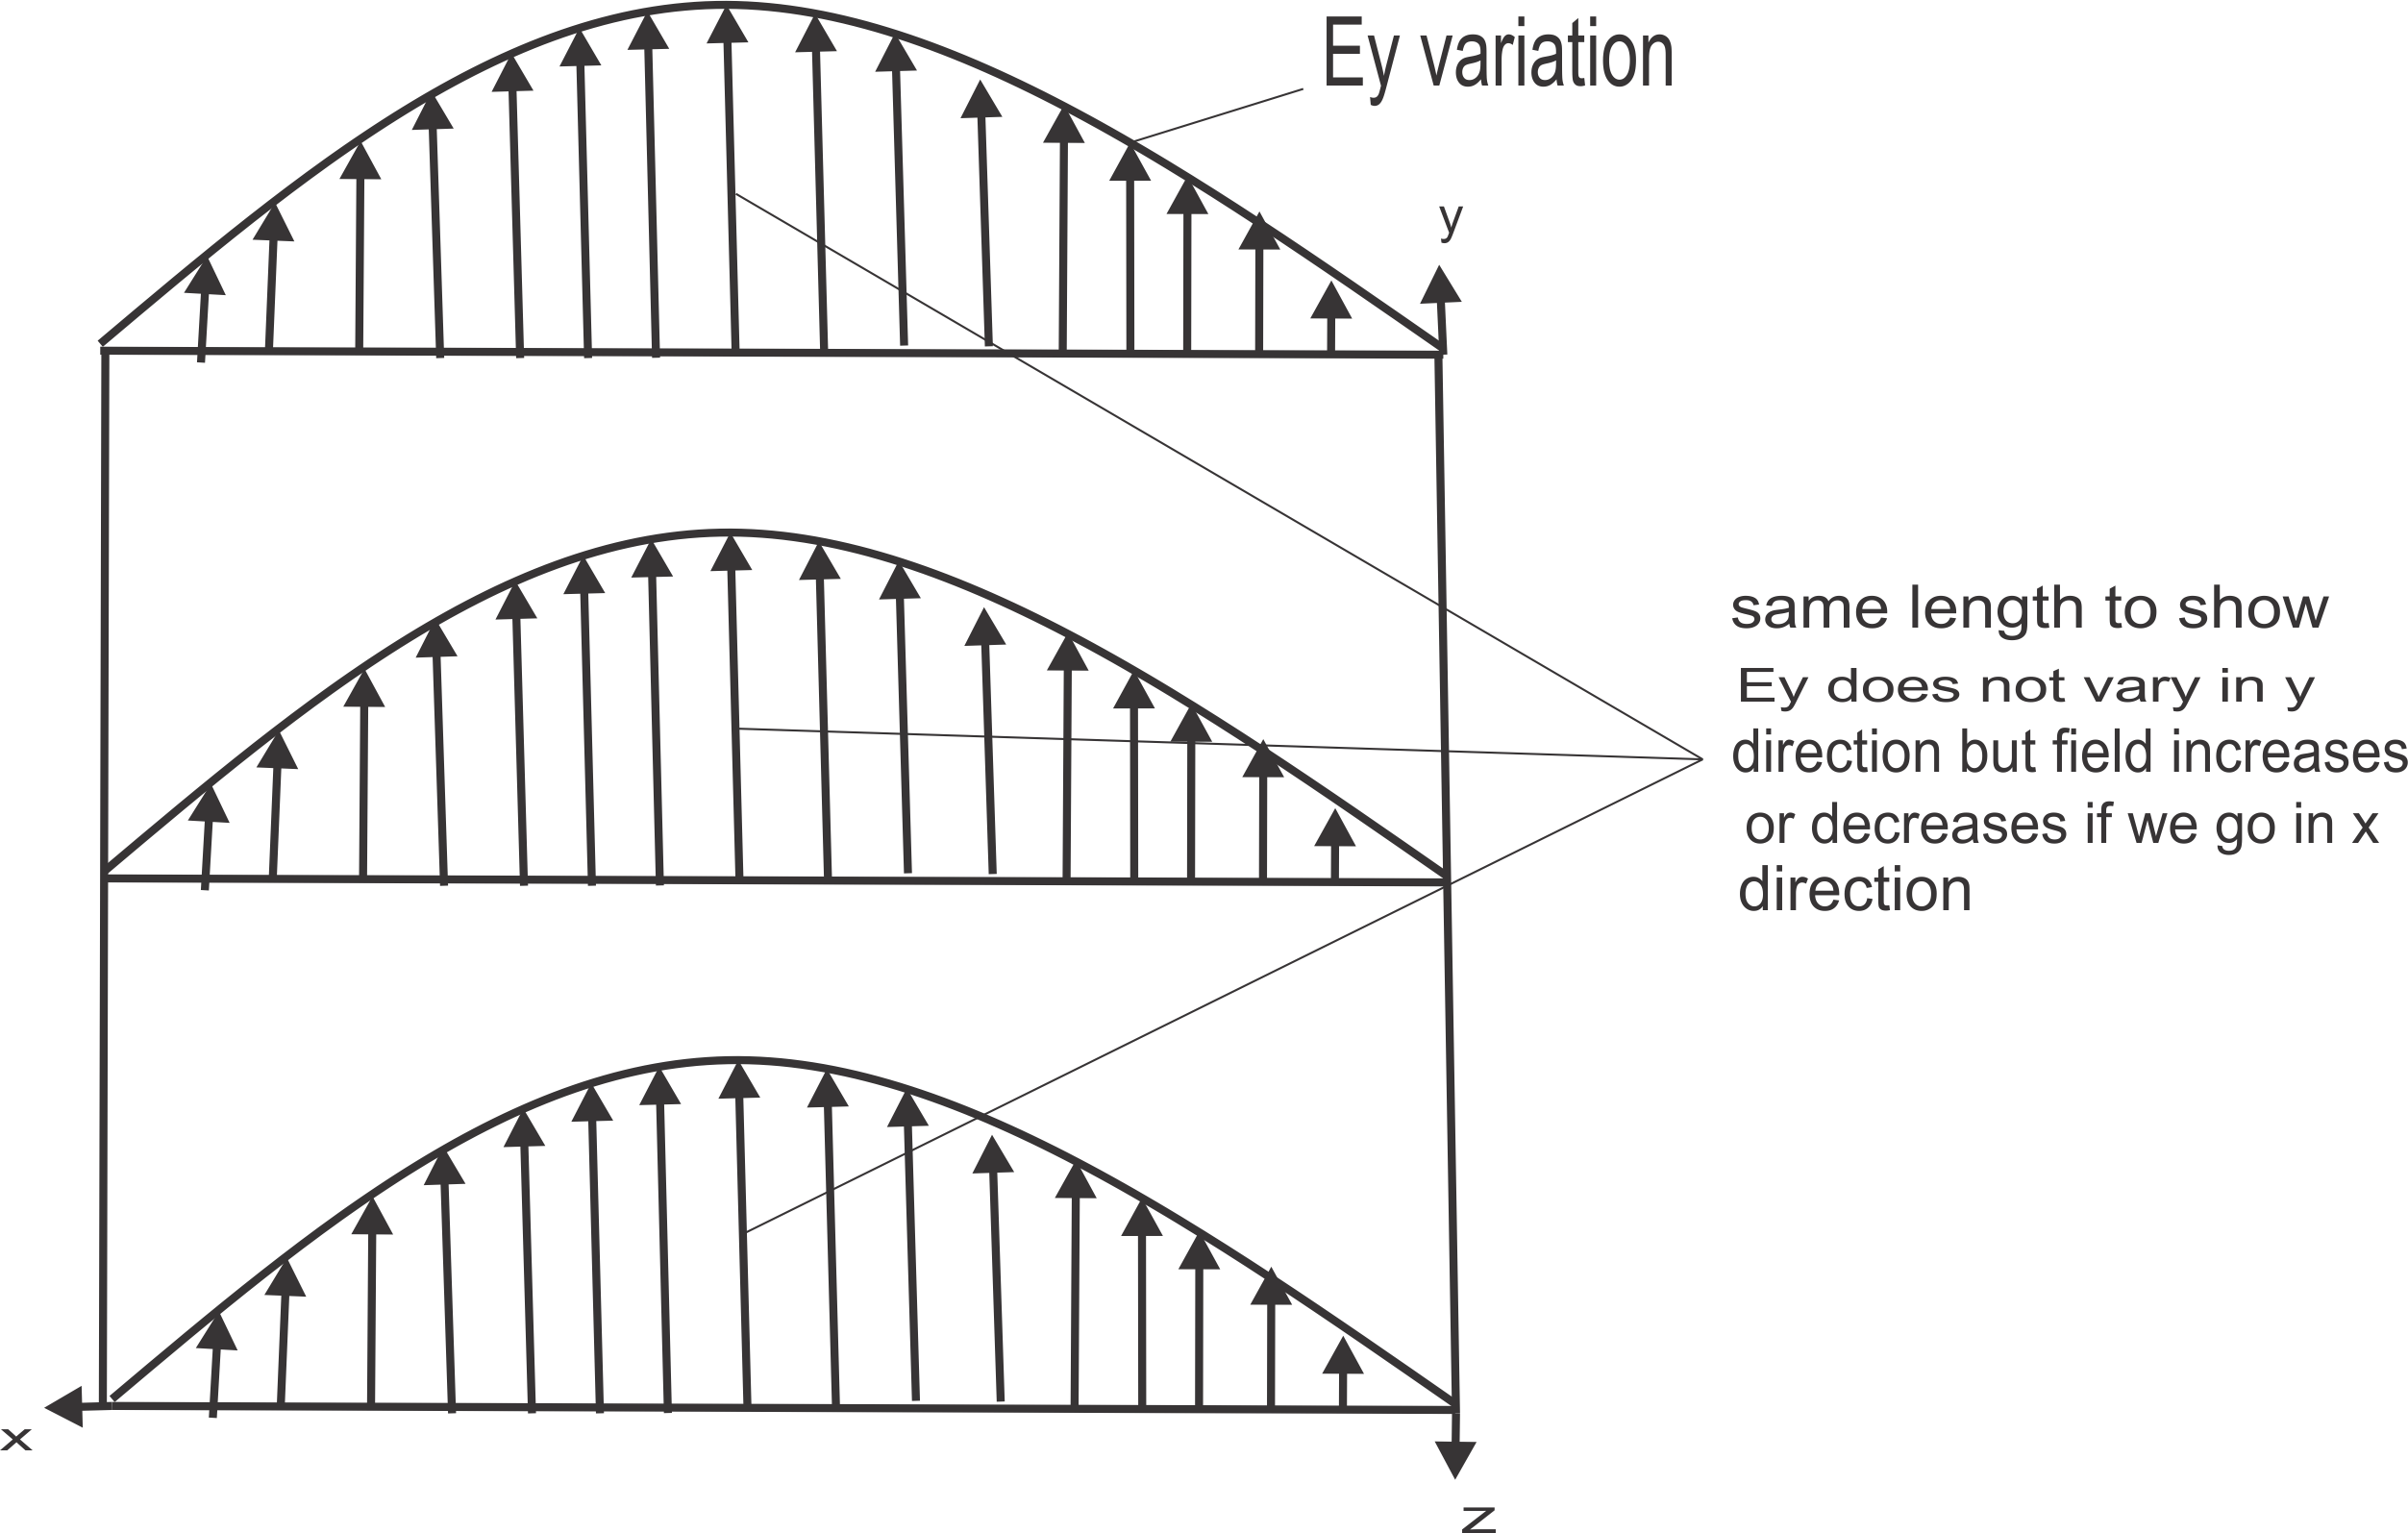
\includegraphics[width=1\linewidth]{./graphics/group39-1}
\caption{Cross section of $E_y$ vector field in the dominant mode at an arbitrary value of z}
\label{fig:lec39-1}
\end{figure}

The field at a y-location is the same in magnitude and direction. However, it varies as we move in the x-direction, maximum at $x = 0$ and at $x = a$. The tangential components of $E_y$ against the side walls is equal to zero, we visualize the detail of these fields in different waveguiding structure later. At the moment, it appears $E_y$ is maximum at the broader wall of the waveguide as shown by the line traced on the waveguide in figure~\ref{fig:lec39-2}. The same will happen to higher modes also you find the locations where the electric and magnetic fields are maximum. Why this information is important is one can ask a question that a waveguide is giving to you. How can a particular mode be excited inside the waveguide? Do we have a mechanism by which a particular order mode can be excited or can we selectively excite certain modes inside a waveguide?
\begin{figure}[h]
\centering
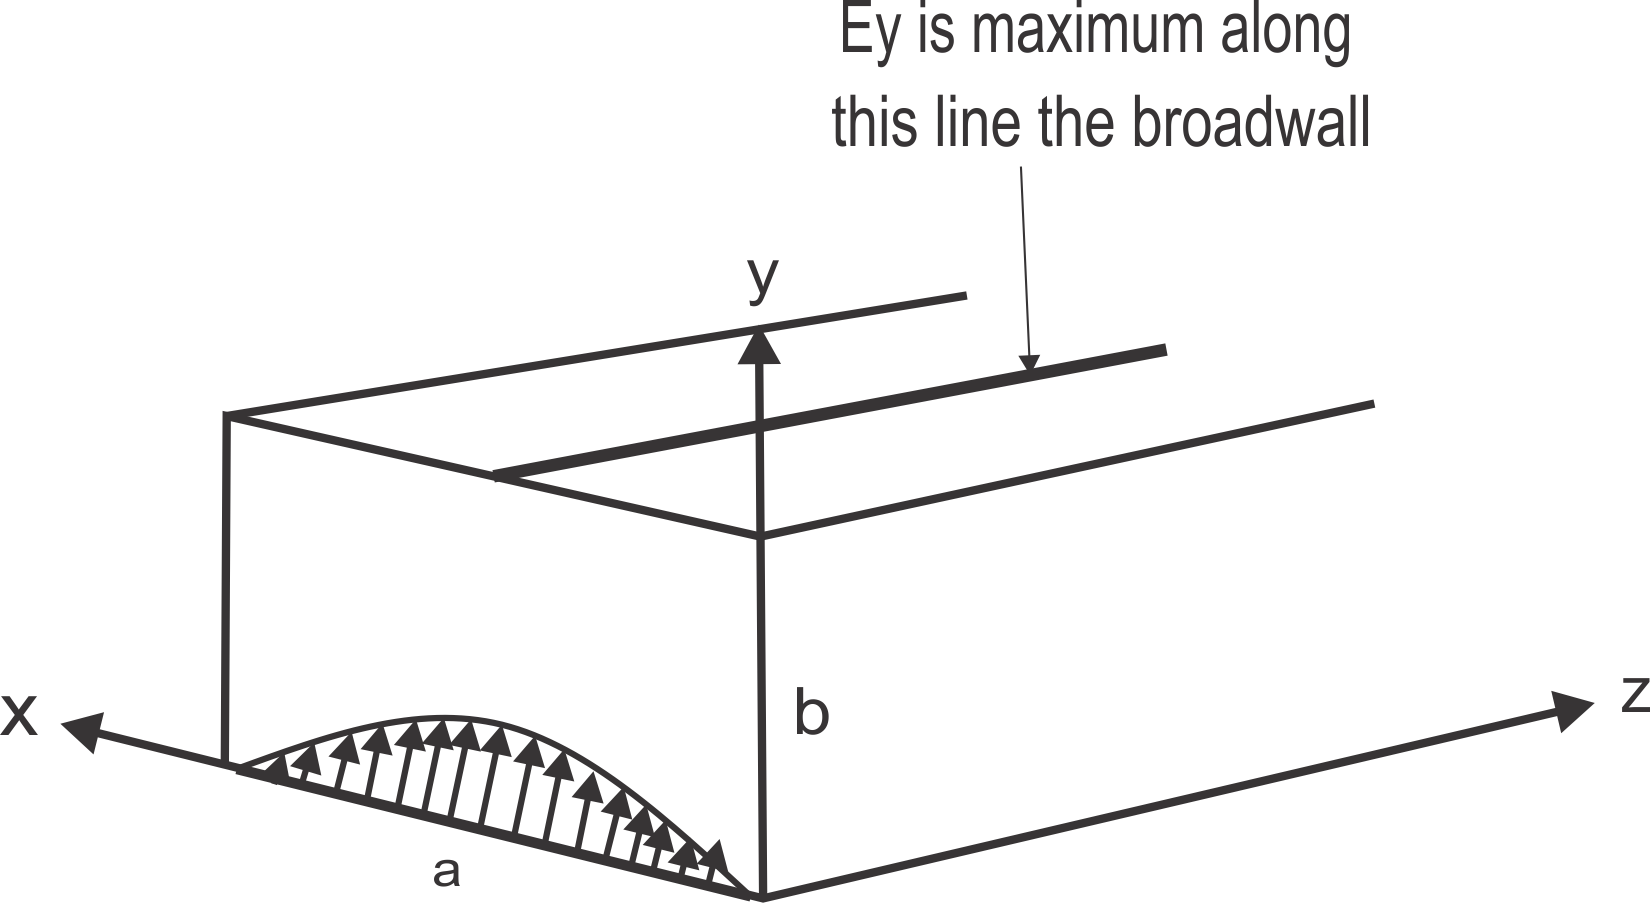
\includegraphics[width=1\linewidth]{./graphics/group39-2}
\caption{Field pattern of $E_y$ along the z direction for the $TE_{10}$ mode}
\label{fig:lec39-2}
\end{figure}

By looking at the field distribution, it becomes clear that yes, if we create a mechanism by which the field is maximum along the line shown in figure~\ref{fig:lec39-2} and as such the mode which will be excited inside the waveguide will be the $TE_{10}$ mode. So two things are required for excitation of this $TE_{10}$ mode, first, the size of the waveguide should be such that the x direction is broader than the y direction and second, the excitation mechanism should be such that the field or mode in which we want to get excited, matches with the excitation i.e maximum at the broader wall for the $TE_{10}$ mode in this case. So for the excitation of the $TE_{10}$ mode, we put some kind of a probe inside the waveguide on the broad wall and because of that, we have a finite field. For $TE_{10}$ mode, we talked about the field distribution satisfies the boundary conditions. We have the point of field excitation as shown in figure~\ref{fig:lec39-3}, and then we show that to satisfy the boundary condition for a field, we require all possible modes for the waveguide either for travelling or decaying.
\begin{figure}[h]
\centering
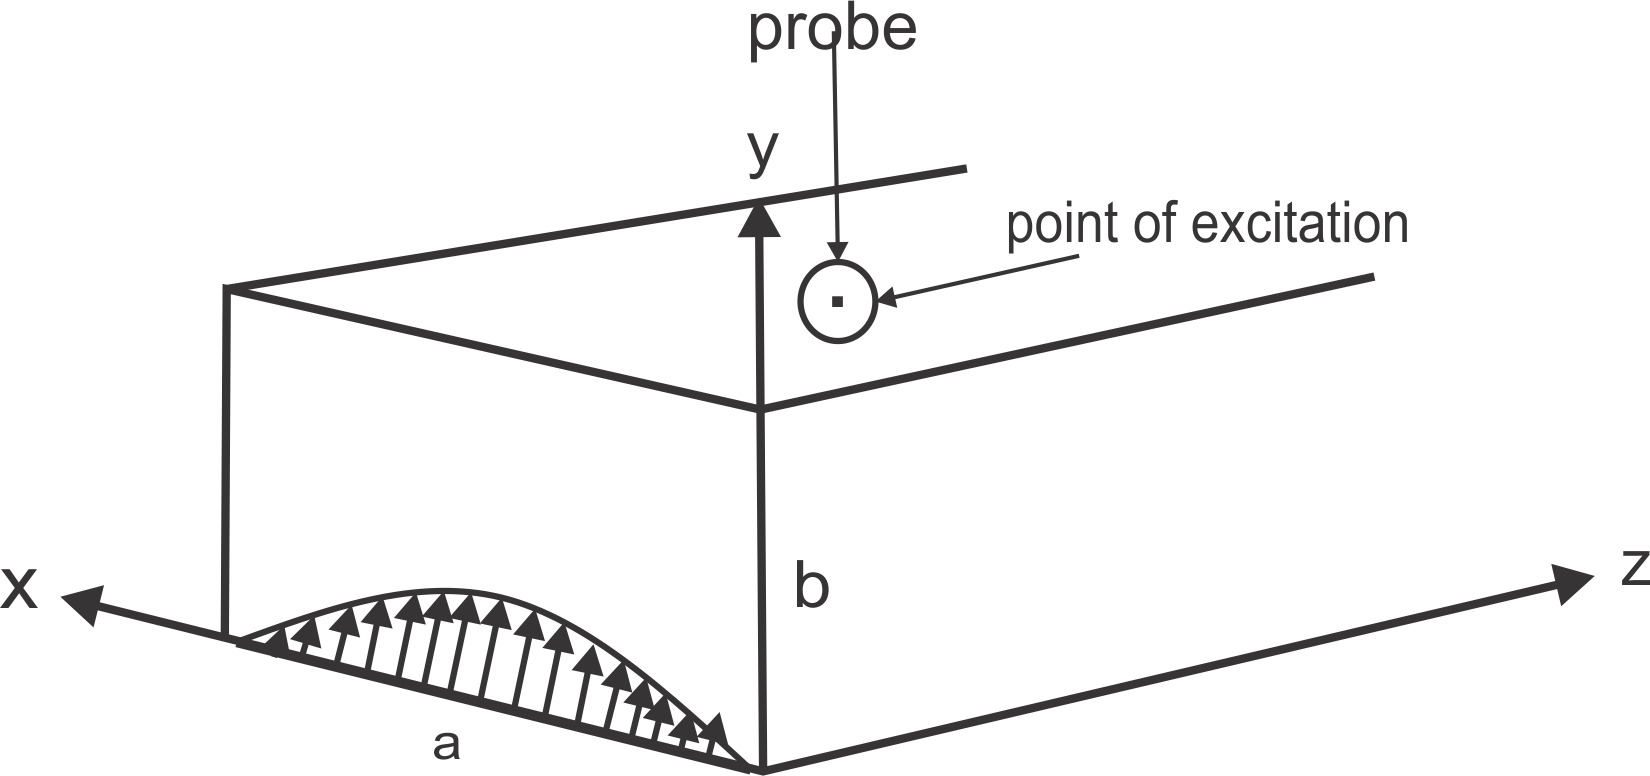
\includegraphics[width=1\linewidth]{./graphics/group39-3}
\caption{Excitation of $TE_{10}$ mode}
\label{fig:lec39-3}
\end{figure}

These are essentially three orthogonal functions which satisfy the boundary condition inside the x structure. So locally around the probe, all kinds of modes get excited inside the waveguide, including the fields which are decaying fields. Only as we travel further in the waveguide, those fields which are below the cut-off will die down rapidly while only that frequency for which the cut-off frequency is less than will travel. If we make sure that this frequency is larger than the cut-off frequency of the $TE_{10}$ mode but smaller than any of the other cut-off frequencies, we get the $TE_{10}$ mode inside the waveguide structure guaranteed. So essentially a $TE_{10}$ mode inside the waveguide can be excited by pulling a probe which can excite an electric field inside the waveguide at the middle of the broader wall.

In practice, whenever we do the experiment, or we carry high-frequency signals like microwave signals, these signals are carried by a rectangular waveguide and this rectangular waveguide always operates in a mode which is the dominant mode of the waveguide called the $TE_{10}$ mode.

One can ask the question, how do we get the saying that we should operate this waveguide in a single-mode operation\index{single-mode operation or propagation}? There are many applications where we want a single-mode operation. The question is why we want a single-mode operation. The answer essentially lies in our dispersion relation. It says that the phase constant is a function of $m$ and $n$ i.e $\beta = \sqrt{{\omega}^2\mu\epsilon - \left(\dfrac{m\pi}{a}\right)^2 - \left(\dfrac{n\pi}{b}\right)^2}.$ Hence the velocity of the mode is a function of m and n. This means that for a given frequency $\omega$, the different modes are going to travel at different speeds. Now to send information on this waveguide, we try to put energy inside this waveguiding structure and then if larger modes can be supported by the waveguide structure when the waveguide is not in single mode operation, the energy will get distributed into various modes i.e various combinations of m and n. Each mode will have its velocity for travelling. So as it travels, the energy which is going on in different modes is essentially separated. Imagine a situation where we transmit signals which are not time-varying sinusoidal signals, say a pulse at high frequency, now if the energy is divided into different modes, and different modes travel at different speeds, then the energy reaches the other side of the waveguide, then all the modes will not reach the other end at the same time. That means the energy packet we send, will not be the energy packet we receive as they will be distributed in time as some modes will arrive earlier, and some modes will arrive later. So the dispersion phenomena we talk about essentially will give us the broadening of the signal in time as it travels on the waveguide. This is happening because energy is being distributed into various modes and different modes travel at different speeds. To avoid this, we try to put the energy only in one mode so that energy remains in that mode and the distribution of energy or differential delays which can be caused because of multiple modes of propagation inside the waveguide is avoided and we do not have a broadening of the signal when it travels on the waveguide, because of multi-mode propagation. This is the aspect one is to make use of when we design the waveguides at high frequencies.

In conclusion, for a rectangular waveguide, the important mode is the transverse electric mode $TE_{10}$ mode, that mode we also call dominant mode\index{dominant mode} because it has the lowest cut-off frequency and for this frequency, we should make sure single-mode propagation takes place over a certain range of frequencies. So in experiments, we make sure the frequency lies in that range so there is a single-mode propagation.
% \chapter{Surface current on the waveguide walls}
In this chapter, we shall establish that the fields we got for rectangular waveguide if we take a limiting case that the fields must represent the ones we got for parallel plane waveguide. Now we do the work of showing that the field we got for a rectangular waveguide can represent the field we got for a parallel plane waveguide in the limiting case when one of the dimensions of the rectangular waveguide becomes infinity. We ask the question what happens to the mode which was $TM_0$ which becomes the TEM mode in the parallel plane waveguide? What happened to that mode in a rectangular waveguide? Does this mode now exists inside the rectangular waveguide or it exists only inside a parallel plane waveguide?
\begin{figure}[h]
\centering
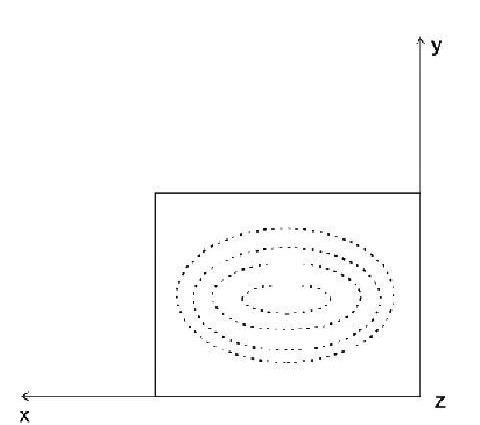
\includegraphics[width=0.6\linewidth]{./graphics/group4001}
\caption{}
\end{figure}
 So we consider the question does a TEM exist inside a rectangular waveguide? Using the rectangular wavelength, we could find out that the electric and magnetic fields are both perpendicular to the direction of propagation. That means they must lie in the XY plane below. That means they must perform a closed loop in the plane. Then there has to be CURRENT enclosed by the magnetic field lines, then and only then can the magnetic field lines survive. Hence there would either be a CONDUCTION or DISPLACEMENT current that will guarantee the survival of the magnetic field lines since we do not have any conducting medium inside the waveguide, it is completely hollow, with pure dielectric inside, and there is no possibility of conduction current enclosed by the magnetic field lines. Hence conduction current is zero inside the rectangular waveguide, so magnetic field lines can only be sustained by the fact that we have a displacement current, and it must be following in the z-direction. This displacement current will also require an electric field going in the z direction which will already say is not there for TEM mode. We said the electric field only lies on the transverse plane for TEM mode. It does not have a component perpendicular to the plane of the paper.

If that is so, we cannot have the displacement current inside the waveguide that is in the z direction, so either we have a conduction current or displacement current going in the Z direction. So there is no current which is flowing perpendicular to the plane of the paper, and hence there is no current sustaining the magnetic field lines. As by amperes law, the magnetic field lines must enclose current. This means that these fields which are lying in the transverse plane cannot exist, as there are no currents to support the magnetic field lines. That means the TEM cannot exist inside a rectangular waveguide, so TEM mode DOES NOT EXIST IN a RECTANGULAR WAVEGUIDE.

Let us take a parallel plane waveguide as a limiting case of a rectangular waveguide. If we take the rectangular waveguide in mode is existing and make ${b=\infty}$, we get a structure mode of only side E and G left, and the wave is going to travel in the Z direction. So if the electrical field was on the plane of the paper and the wave is going to propagate in the Z direction, this would essentially correspond to the TE mode. So with sides, E and G left and an electric field on the plane of the paper in the Y direction, we would get a geometry which is the parallel plane geometry which gives the TE mode. We can understand better from the diagram shown below.
With an electric field in the Y direction as shown below,\\
${E_x = E_z = 0 \qquad E_y = - \dfrac{j\omega\mu a}{\pi} Csin(\dfrac{\pi x}{a})e^{-j\beta z}}$\\
$H_x = + \dfrac{j\beta a}{\pi} Csin(\dfrac{\pi x}{a})e^{-j\beta z}$\\
$H_y = 0\qquad H_z = Ccos(\dfrac{\pi x}{a})e^{-j\beta z}$ and magnetic field ${H_x}$ and ${H_z}$ for this case had.
\begin{figure}[h]
\centering
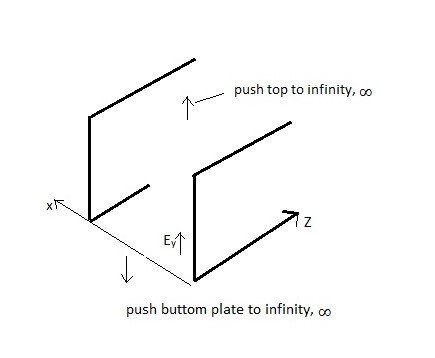
\includegraphics[width=.7\linewidth]{./graphics/page3}
\caption{}
\end{figure}
and all these fields were constant as a function of Y.Some thing we can get now with ${b=\infty}$ that is there are no boundary conditions to apply in the Y direction. The field is infinite, then ${E_y}$ is constant along Y direction. That is precisely the field we used to get a parallel plane waveguide. So in rectangular waveguide,we can take ${TE_{10}}$ mode and make b in infinity and since we do not have any dependence of E here on y,it means that the fields in the ${TE_{10}}$ case are essentially the same for a parallel plane waveguide. So the ${TE_1}$ mode of a parallel plane waveguide has essentially the same field as ${TE_{10}}$ mode of a rectangular waveguide, Now we have a Z magnetic field in the z-direction. So in the limiting case of the ${TE_{10}}$ mode,we can get the transverse electric mode lowest order transverse electric mode which is $TE_1$ mode and it will be exactly what we got for ${TE_{10}}$. Another mode we had was the TEM mode for which the electric field was not tangential to the boundaries,(i.e along x above)the magnetic field was tangential to the boundary (alone y direction)and we say that was the mode which was not dispersive and travels as if the conducting boundary are not existing and that was the mode which was the TEM mode. We had the diagram below that if we take a parallel plane waveguide, the electric and magnetic field is shown in the direction below. 

The wave travels without any variation of the electric and magnetic field as we saw earlier because neither H requires the boundary conditions to be satisfied which is tangential, so we can always have surface currents, nor the normal components of an electric field needs only boundary condition to be satisfied.We can always have the surface charge induced to compensate for the normal component of the electric field.So this mode which was the TEM mode was existing inside the parallel plane waveguide.
\begin{figure}[h]
\centering
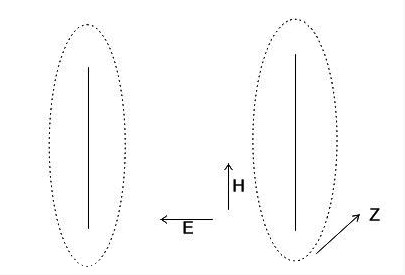
\includegraphics[width=.7\linewidth]{./graphics/page4}
\caption{}
\end{figure}
One can ask the question that if the figure above was the limiting case of the rectangular waveguide, how come this mode exist in the parallel plane waveguide,but when we take a rectangular this mode does not exist!We argue that since the magnetic field is in the Y direction and the plane is extended in the Y direction and this means the magnetic field lines essentially close at infinity and enclose the conductions shown by dotted lines.These conduting plane have a surface current flowing on them.In the case of rectangular waveguide were those boundaries are finite,the magnetic field closed on themselves and current is enclosed.That is why the TEM mode cannot exist in rectangular waveguides.But with a parallel plane structure,the magnetic field lines will close at infinity and will enclose the plane conductors as shown above and so the TEM mode can exist inside a parallel plane waveguides.This is the mode like we say in two conductor system like coaxial cables,this mode propagates.

So whenever we have a two conductor system,the lowest mode which will propagate will be TEM mode,however if we go to the rectangular waveguide,the lowest mode which will propagate will be ${TE_{10}}$ mode.The important conclusion to draw is that whenever we have a hollow structure,like a hollow pipe kind of waveguide,tyhe TEM mode cannot exist which is non dispersive.It is a special mode that is not supported by the rectangular waveguide. That is why we have all the problem of dispersion and so on,inside a rectangular waveguide. The parallel plane waveguide is still a structure which is infinite in extent,it cannot be realized in practise.It is good for understanding,but when we want to realize the structure in practise,it is the rectangular waveguide which can be realized practise,not the parallel plane waveguide,so whenever if we have a physical structure which is a rectangular waveguide,we always have a cut off frequency associated with that and we always have problem like dispersion and so on,associated with them.

With this understanding,let us try to see the current which gets excited on the walls of the waveguide,which actually support these fields inside the waveguide.So whether we take a parallel plane or rectangular waveguide,what is the mechanism by which these fields are supported inside the waveguide? what are the sources? The sources are nothing but surface charge and surface currents which lie on the inner surface of the waveguides.So as the wave travels even the surface charge keeps moving i.e accumulate at different locations as we see later and these charges and surface currents supports the electric and magnetic field inside the waveguide which is responsible for carrying power inside the waveguiding structure.So what we do now,is first we try to visualize the fields which would be inside the waveguide and then try to visualize how the currents are disturbing on the walls of the waveguide, so let us take the simplest case which is the TEM case for a parallel plane waveguide in the parallel plane waveguide shown for TEM mode,the electric field E is perpendicular to the plans.With\\
${E_y = Ce^{-j\beta z}}$ and ${H_x = \dfrac{C}{\eta}e^{-j\beta z}}$ We can visualize these fields.if we tried out how these fields are going to be a function of space and time in the structure.First we freeze time,remember all the qualities above are intrinsic function of time.So ${e^{j\omega t}}$ is implicit in all the terms\\
$E_y = Ce^{-j\beta z}e^{j\omega t}\qquad H_x = {\dfrac{C}{\eta}}e^{-j\beta z} e^{j\omega t}$
\begin{figure}[h]
\centering
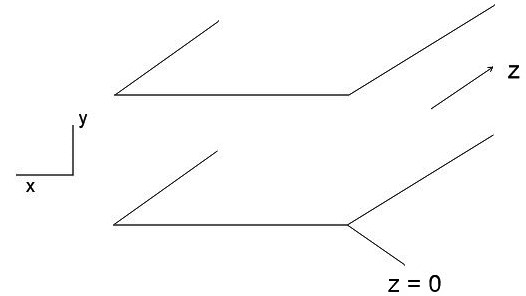
\includegraphics[width=.7\linewidth]{./graphics/page6}
\caption{}
\end{figure}

So these fields are varying as a function of space and time,so if we stand at a particular location in space, the field will vary as a function of time.if we freeze time or say at any instant of time,we look along the waveguide,we see a variation given as ${e^{-j\beta z}}$ so to visualize these fields in 3D, first we freeze time i.e make ${Wt}$ constant.At that instant,we want to see how the field are disturbed in space. Once we get those fields disturbing in space, then we essentially say that these field will be moving with a phase velocity for the mode. Then the electric field drift inside this waveguide with the phase velocity. So when we visualize these fields, essentially we try to visualize the spatial variation of the fields at some instant of time and without loosing generally,we can take the time t=0. If we take t=0, i.e freeze time,then the field visualization is simply the real part of ${H_y}$ and${H_x}$ which is \\
${Re\{Ce^{-j\beta z\}}\}}$ and ${Re\{\dfrac{C}{\eta}e^{-j\beta z}}\}$ That is ${Ccos\beta z}$ and ${\dfrac{C}{\eta}cos\beta z}$ If we consider points Z=0,with variation of ${\beta z}$
so the field varies as a cosine function in direction Z. It is constant in XY plane, so we see the cosine variation along the Z direction for these fields.The electric field is same at any Z(i.e XY plane)and in the Y direction.
\begin{figure}[h]
\centering
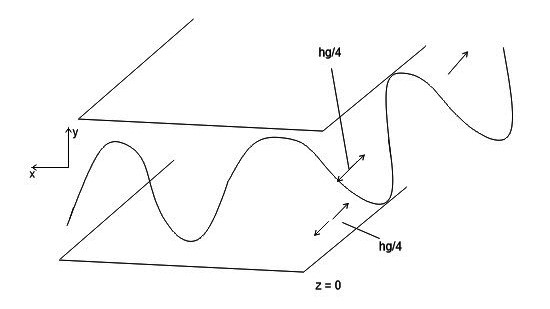
\includegraphics[width=.7\linewidth]{./graphics/group4002}
\caption{}
\end{figure}
\begin{figure}[h]
\centering
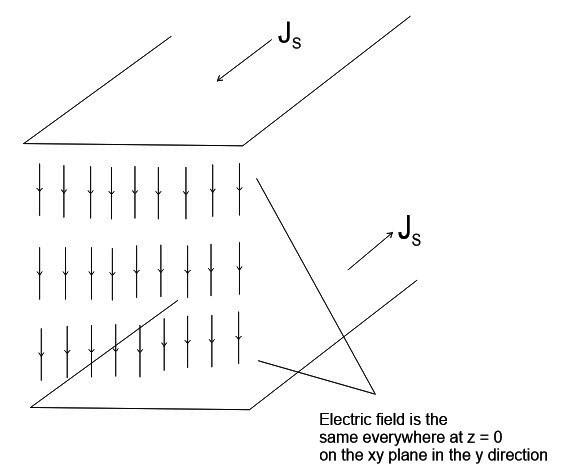
\includegraphics[width=.7\linewidth]{./graphics/page702}
\caption{}
\end{figure}
\begin{figure}[h]
\centering
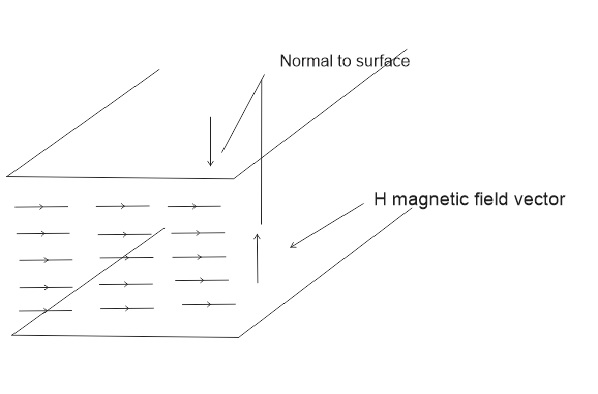
\includegraphics[width=.7\linewidth]{./graphics/page703}
\caption{}
\end{figure}

The magnetic field is same at Z(XY PLANE)and in the X direction.The E and H direction is maintained to show the direction of propagation by poynting theorem(a british physicist John Henry Poynting). So E start maximum will H maximum at Z=0 \quad${A\quad Z= \dfrac{hg}{4}}$they have reduced to zero. Beyond ${Z= \dfrac{hg}{4}}$,they change direction and start increasing till they go to another maximum at ${Z=\dfrac{hg}{2}}$ They again start decreasing from the direction of ${Z=\dfrac{hg}{2}}$ to ${Z=\dfrac{3hg}{4}}$where E and H are zero.Beyond ${Z=\dfrac{3hg}{4}}$,  they change direction once more and start increasing getting to Z=0 state at ${\lambda g}$.With little practice one can see how the electric and magnetic field varies inside the waveguide.Now we know that if that if the magnetic field pattern is as shown above,the current which is going to flow in the surface of the conductor is related to the magnetics fields i.e the tangential component of the magnetic fields.The ${\hat{n}\times\bar{H}}$.gives the surface currents on the conducting walls. Since we are considering here ideal conductors,essentially,calculating ${\hat{n}\times\bar{H}}$, that is the current which is truely confirm to the surface of this parallel plane waveguide. 

The normal to surface of H fields is shown. We choose the normal pointing inwards as that is the part that bounds the electromagnetic wave to be propagated.The normal opposite that would be the electromagnetic wave was propagated outside the conducting plane. So the unit vector of the wave plane is going upward in ${\hat{y}}$ direction for the upper plane in ${-\hat{y}}$ direction. Now we can calculate ${\hat{n}\times\bar{H}}$. The ${\hat{n}\times\bar{H}}$ will give the direction of surface current,which top plane, ${\hat{n}\times\bar{H}}$ is -Z direction as to say the surface current is coming out from top plane and going in the bottom plane.Hence ${J_s}$ direction shown on the top and bottom plane respectively.${J_s}$ will be having same variation as the variation of the magnetic field. Maximum at Z=0, and ${Z= \dfrac{hg}{4}}$.Maximum at ${Z=\dfrac{hg}{2}}$ but with direction reversed, zero at ${\dfrac{3hg}{4}}$ and maximum again at ${Z=hg}$

with same direction as with Z=0. So in a two conductor system, we get current flow in the direction in which the wave is propagating. ${J_s}$ in the +Z direction in the bottom at Z=0 and ${J_s}$ in -Z direction at the top for Z=0. If we have a two conductor system like the coaxial cable,we connect a voltage source,current goes inside the conductor and returns back through what is called a ground path.So we see that the current goes inside from one terminal and comes outside from the other terminal. So in that situation of the two conductor system, the direction of the current flow which we have for the TEM mode(keep in mind) is the same as the direction of wave propagation.So current is going from bottom plane and returning from top plane at Z=0.The question me ask is if the wave is propagating in the Z direction ,is it always true that current has to flow in the Z direction or direction of wave propagation? Then we got the answer which is wrong.That is since we always discuss the transverse electromagnetic mode.
\paragraph{}The fact that we are used to when we go to low frequency circuit,immediately we jump to the conclusion that yes since the wave is moving in the Z direction,the power is flowing in the Z direction,the current must flow in that direction.
\begin{figure}[h]
\centering
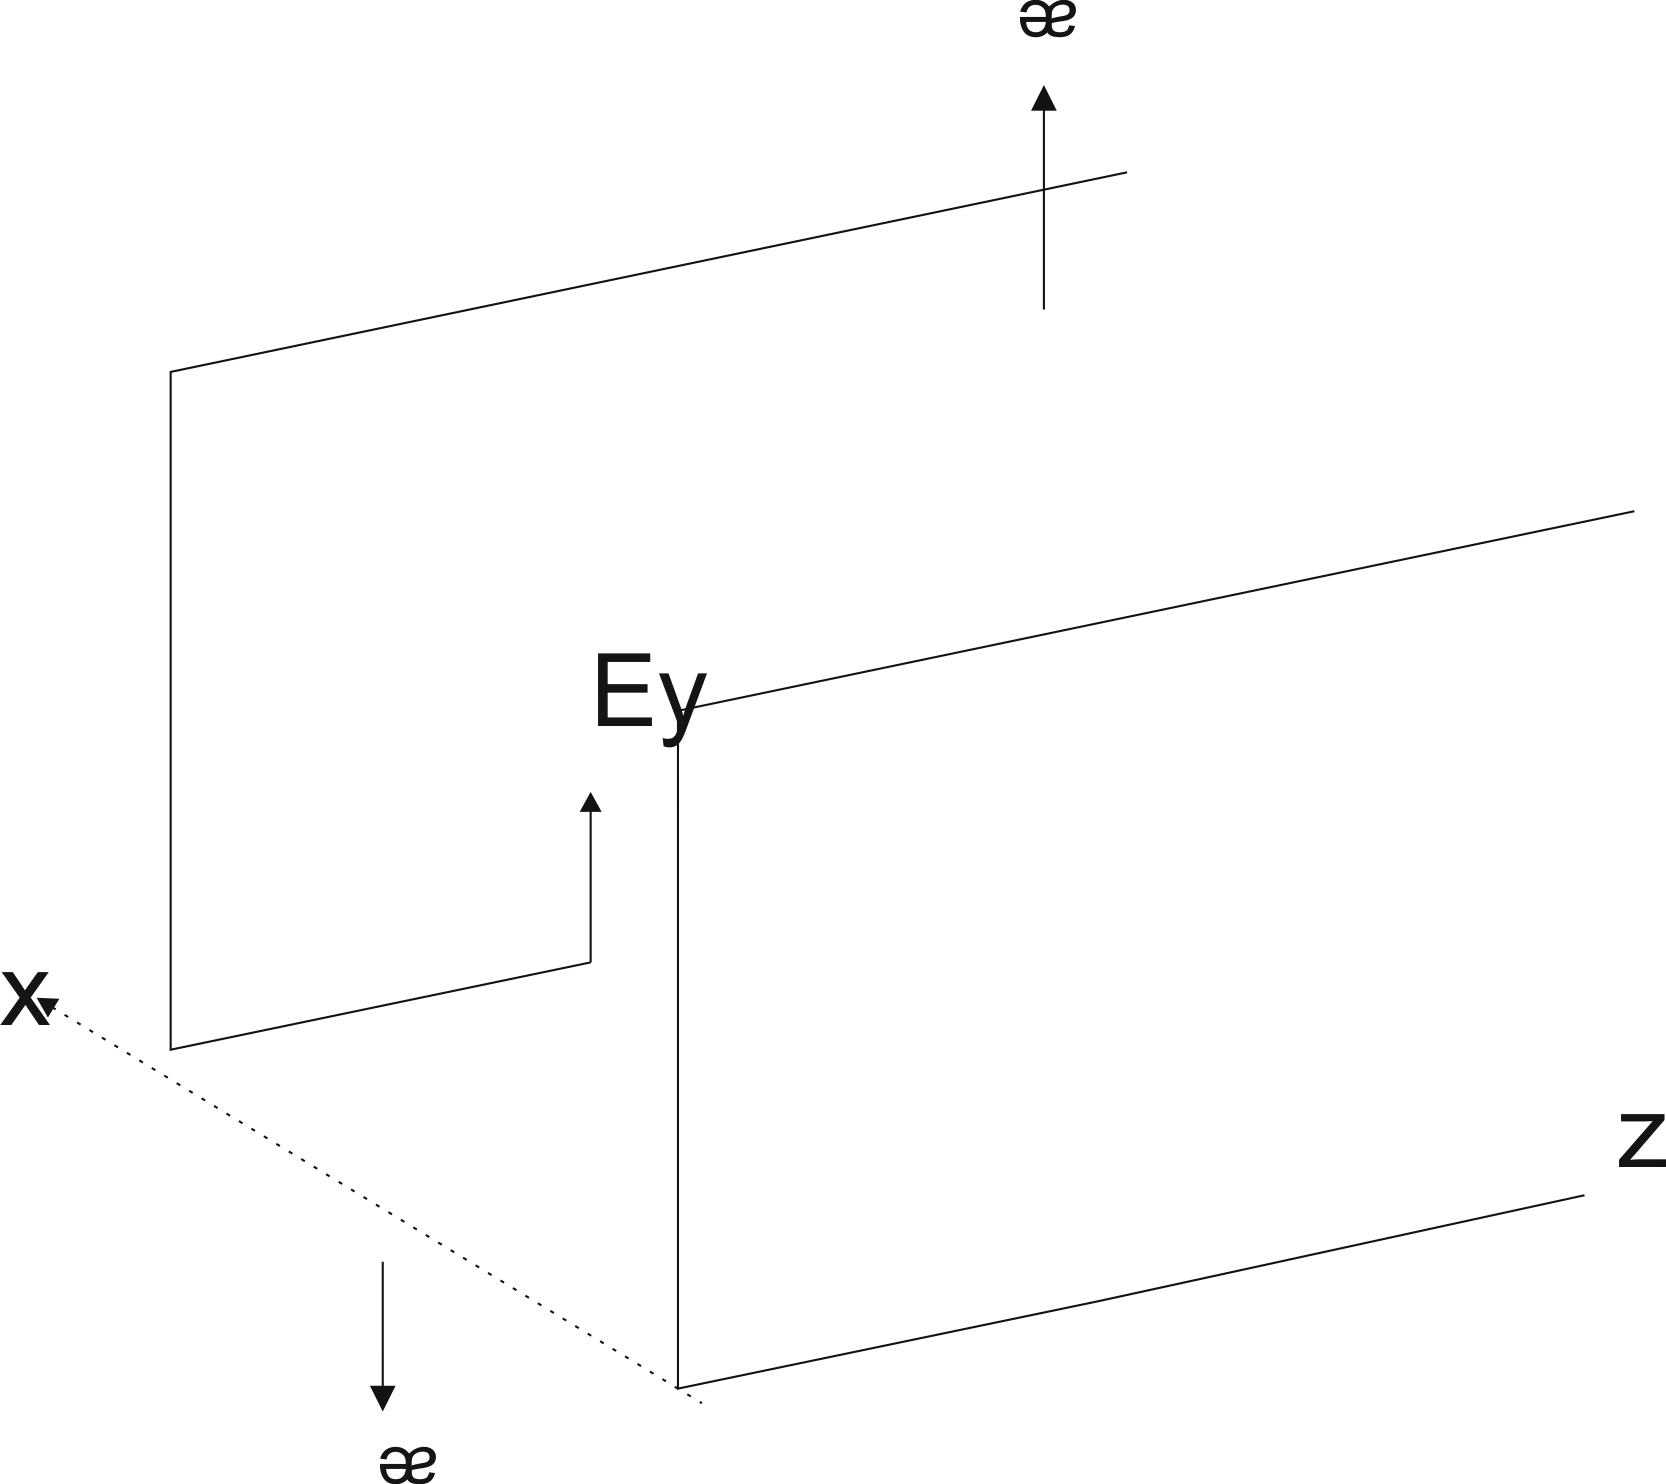
\includegraphics[width=.7\linewidth]{./graphics/WATSON4}
\caption{}
\end{figure}
\paragraph{}Let us look at the parallel plane waveguide,let us take a mode which is TE mode and let us see what will be the direction of current and field in the waveguide.As we saw ,the fields for the parallel plane waveguide is identical to the $TE_{10}$ mode for rectangular waveguide giving as\\
${E_x = E_z = H_y = 0}$\\
$E_y = -\dfrac{j\omega \mu a}{\pi}Csin(\dfrac{\pi x}{a})e^{-j\beta z}$\\
$H_x = -\dfrac{j\beta a}{\pi}Csin(\dfrac{\pi x}{a})e^{-j\beta z}$\\
$H_z = Ccos(\dfrac{\pi x}{a})e^{-j\beta z}$

So the electric field will be y oriented,it will have a variation which would be in the Z direction. With very in the Z direction with the value of ${\beta}$.To visualize ${E_y}$, lets take the real part of ${E_y}$ and look at its variation,and with respect to x,y and z. This will give us a 3 dimensional picture of the fields.\\
$E_y = \dfrac{-j\omega \mu a}{\pi}Csin(\dfrac{\pi x}{a})e^{
-j\beta z}\equiv e^{-j\dfrac{\pi}{2}}\dfrac{\omega \mu a}{\pi}Csin(\dfrac{\pi x}{a})e^{-j\beta z}$\\
${E_y = \dfrac{\omega \mu a}{\pi}Csin(\dfrac{\pi x}{a})e^{-j(\beta z + \dfrac{\pi}{2})
}}$\\
Real ${(E_y) = \dfrac{\omega \mu a}{a}Csin(\dfrac{\pi x}{a})cos(\beta z + \dfrac{\pi}{2})}$\\
${[cos(-(\beta z + \dfrac{\pi}{2}))=cos(\beta z + \frac{pi}{2})]}$\\
cosine is even function\\
${\dfrac{\omega \mu aC}{\pi}\equiv A}$, we have Real ${(E_y = Asin(\dfrac{\pi x}{a})cos(\beta z +\dfrac{\pi}{2})}$ ,
Real ${(E_y)= Asin(\dfrac{\pi x}{a})sin(\beta z)}$\\
${= Asin(\dfrac{\pi x}{a})sin(\dfrac{2\pi z}{hg})}$ we can do some thing for ${H_x}$\\
Real${(H_x)= Bsin(\dfrac{\pi x}{a})sin(\dfrac{2\pi z}{hg})}$\\
Real${(H_z)= Ccos(\dfrac{\pi x}{a})cos(\dfrac{2\pi z}{hg})}$\\
Real${(E_y)= Asin(\dfrac{Hx}{a})sin(\dfrac{2\pi z}{hg})}$
 These are the field which are in existence when time is fixed,say at t=0. At that instant, these three expressions gives the fields along the waveguides.\\
 As we can see in the Z direction,the field are all sinusoidal with a spatial period of ${hg}$. However ${Re\{H_x\}}$ and ${Re\{H_z\}}$ are in QUADRATURE. That is ${90^{o}}$ degree out of phase with each other. So when ${H_x}$ is maximum,${H_z}$ is zero.When ${H_z}$ is maximum,${H_x}$ is zero. So in space we have two components now, the ${H_x}$ and the ${H_z}$ components.${H_x}$ component has sine variation along Z,with Z=0, ${H_x}$ is zero at that location, but ${H_z}$ in Z direction is maximum at that location. If we go ${Z=\dfrac{hg}{4}}$, ${H_x}$ is maximum and ${H_x=0}$. Looking from the top, it will appear.
\begin{figure}[h]
\centering
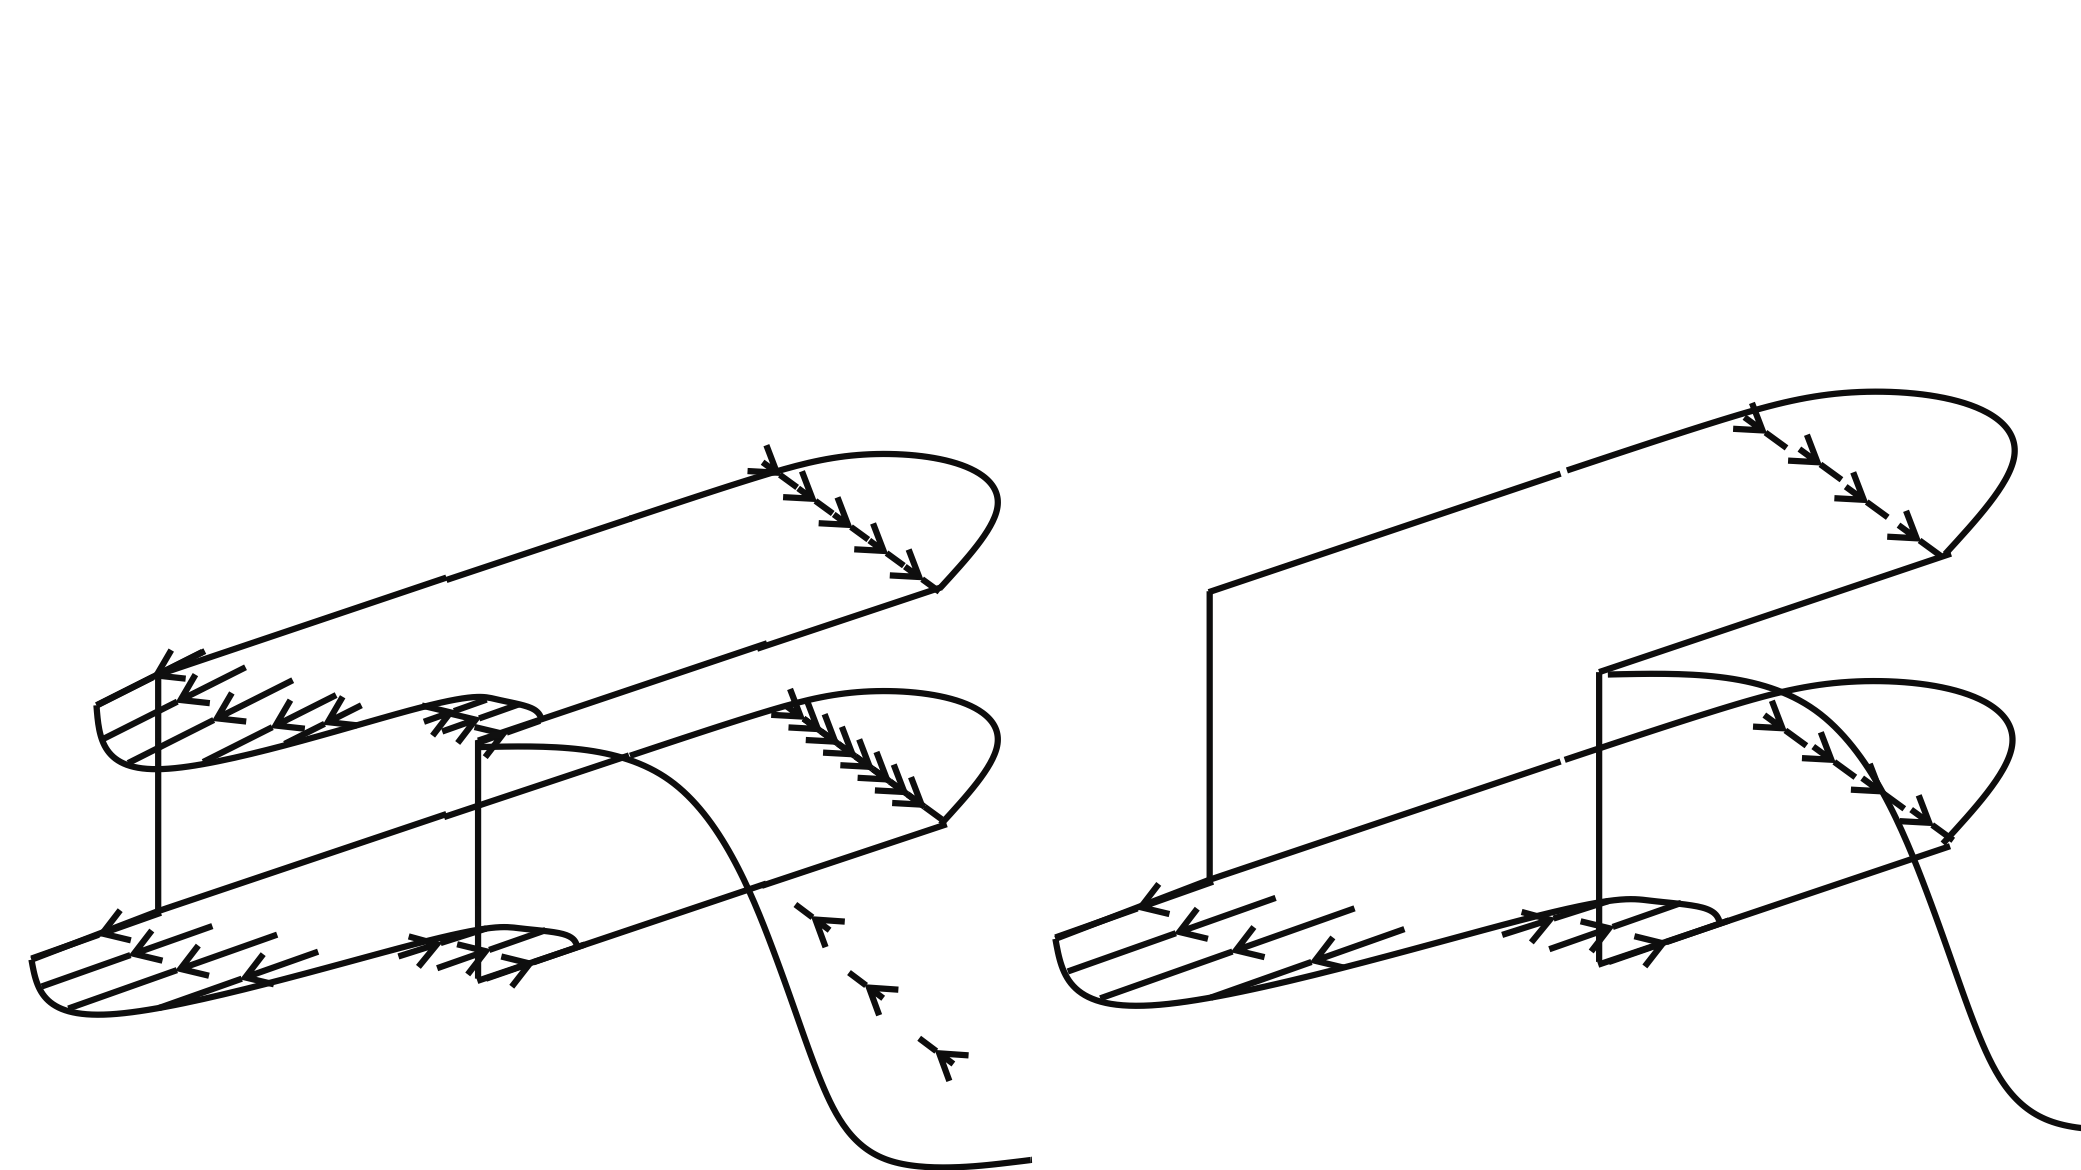
\includegraphics[width=1\linewidth]{./graphics/WATSON}
\caption{}
 \end{figure}
 From the top for this parallel plane waveguide,we see the magnetic fields below.Since the magnetic field close on themselves,it is only a matter of imagination.
 % \begin{figure}[h]
 %	\centering
 %	\includegraphics[scale=0.1]{""}
 %	\caption{}
% \end{figure}
to close the magnetic field loops as shown by the dotted lines ${\dfrac{hg}{4}}$ from here the direction with reverse to have the dotted line from $\dfrac{hg}{4}$  to $\dfrac{hg}{2}$ and so on.
 % \begin{figure}[h]
 %	\centering
 %	\includegraphics[scale=0.8]{""}
 %	\caption{}
 %\end{figure}

Hence we can complete this to get the field distribution below, for a waveguide going from ${-\infty}$ to ${+\infty}$.\\
So from the top in a parallel plane waveguide, the magnetic field lines look like rolled carpets which are scattered inside the structure. They are of infinite length perpendicular to the plane of the paper. This is how the magnetic field will be distributed.

However for the electric field, ${E_y= Asin(\dfrac{\pi x}{a})sin(\dfrac{2\pi z}{hg})}$ the electric field has variation in the Z direction since as ${H_x}$,but it is oriented in the y direction.So from top the electric field lines is perpendicular to the plane of the paper. The behave of ${E_y}$ and ${H_x}$ is identical. That means whenever ${H_x}$is maximum,${H_y}$ will be maximum.So it has identical variation to ${H_x}$.

So if we look at the ${H_x}$ component, so electric field is maximum at ${Z= \dfrac{gh}{4}}$ and minimum at Z=0 with the ${H_x}$ variation along Z.Electric field always point in y direction with wave propagating in the Z direction and ${H_x}$ in the x direction, ${H_y}$ from ${E\times H= Z}$ must point in the y direction at that point.

So we have certain notion we have we have built for electrical circuit that is essentially from the transverse nature of electromagnetic wave. As soon as we make the departure from transverse electromagnetic wave to a transverse electric or transverse magnetic case,all those notion completely breaks down and we get much clearer picture of propagation of electromagnetic waves and the current and the distribution of charges and so on for various configurations.So with this understanding of the current flow for a parallel plane structure which is rather the simplest structure,now we can discuss the field distribution inside a rectangular waveguide which is more practically structure.

In summary, we saw that the TEM mode cannot exist inside a rectangular waveguide. We also show that with a rectangular waveguide and pushing one of the dimensions to infinity, then the field we get for rectangular waveguide are identical to what we have got for a parallel plane waveguide.Then we developed a mechanism of visualizing these field inside a waveguide. We saw two cases, one was of transverse electromagnetic wave in a parallel plane wave guide, the other was the ${TE_1}$ mode inside the parallel plane waveguide. 

% \chapter{Rectangular Waveguide(3)}
%\begin{figure}
%	\centering
%	\includegraphics[width=1\linewidth]{Schematic-of-a-rectangular-waveguide-extending-along-z-a-and-the-TE10-top-and-TE11}
%	\caption{}
%	\label{fig:schematic-of-a-rectangular-waveguide-extending-along-z-a-and-the-te10-top-and-te11}
%\end{figure}
In the previous lecture we try to visualize electric field inside a parallel plane waveguide. We also investigated the modal characteristics of a rectangular waveguide. We found that the modes which first propagate on a rectangular waveguide is a transverse electric mode with index (1, 0). We call that the DOMINANT MODE OF RECTANGULAR WAVEGUIDE. 
	
We also argue that most of the time we went on to operate in this single mode or dominant mode on the waveguide to avoid dispersion i.e broadening of the signal in time domain and as it travels on a guided structure. So this $TE_{10}$  is the most important mode for a rectangular waveguide, because most of the times, the energy is going propagate in this mode. So when this conduct experiments in the laboratory or we go to the fields, most of the time we deal with dominant mode,  $TE_{10}$ mode.


In this lecture we shall see the modal properties of the $TE_{10}$, mode and visualize the fields for $TE_{10}$ mode and then go to  calculation of what is called attenuation constant of  a waveguide. Because whenever we have a particular structure, we never have an
ideal dielectric in practice or ideal conductors. As a result there is always a loss in the walls of waveguides and also losses in the medium which is filling the waveguides.
So after visualizing the fields for $TE_{10}$ mode, in the waveguide, then we go to the calculation of attenuation constant in the rectangular waveguides.

We recall that for the rectangular waveguide,
\begin{equation}
E_{x} = E_{z} = H_{y} = 0
\end{equation}	
\begin{equation}
E_{y} = \dfrac{-j\omega\mu a }{\pi} C\sin \dfrac{\pi a}{x} e ^{-j\beta z}
\end{equation}
\begin{equation}
H_{x} = \dfrac{-j\omega a}{\pi} C \sin\dfrac{\pi a}{x}
	e^{-j\beta z} 
\end{equation}
\begin{equation}
H_{z} = C\cos \dfrac{\pi x}{a} e^{-j\beta z}
\end{equation}
There was no Y component for magnetic field. There was no Z component for electric field. We tried to visualize the fields for parallel plane waveguide, we get something like 
\begin{equation}
Re[E_{y}] = A\sin\dfrac{\pi x}{a} \sin\dfrac{2\pi}{\lambda g}z
\end{equation}	
\begin{equation}
Re[H_{x}] = B\sin\dfrac{\pi x}{a} \sin\dfrac{2\pi}{\lambda g}z
\end{equation}
\begin{equation}
Re[H_{z}] = C\cos\dfrac{\pi x}{a} \cos\dfrac{2\pi}{\lambda g}z
\end{equation}
Essentially this were the fields we visualized inside a
parallel plane waveguide.
\begin{equation}
Re[E_{y}] = A\sin\dfrac{\pi x}{a} \cos\dfrac{2\pi}{\lambda g}z
\end{equation}
if Z = 0, $E_{y}$ is zero. At a distance $ Z = \frac{\lambda g}{4}$, $E_{y}$ is maximum for variation in Z.

If we move the origin such that $Z = \frac{\lambda g}{4}$ is now the starting point shown.
\begin{figure}[h]
\centering
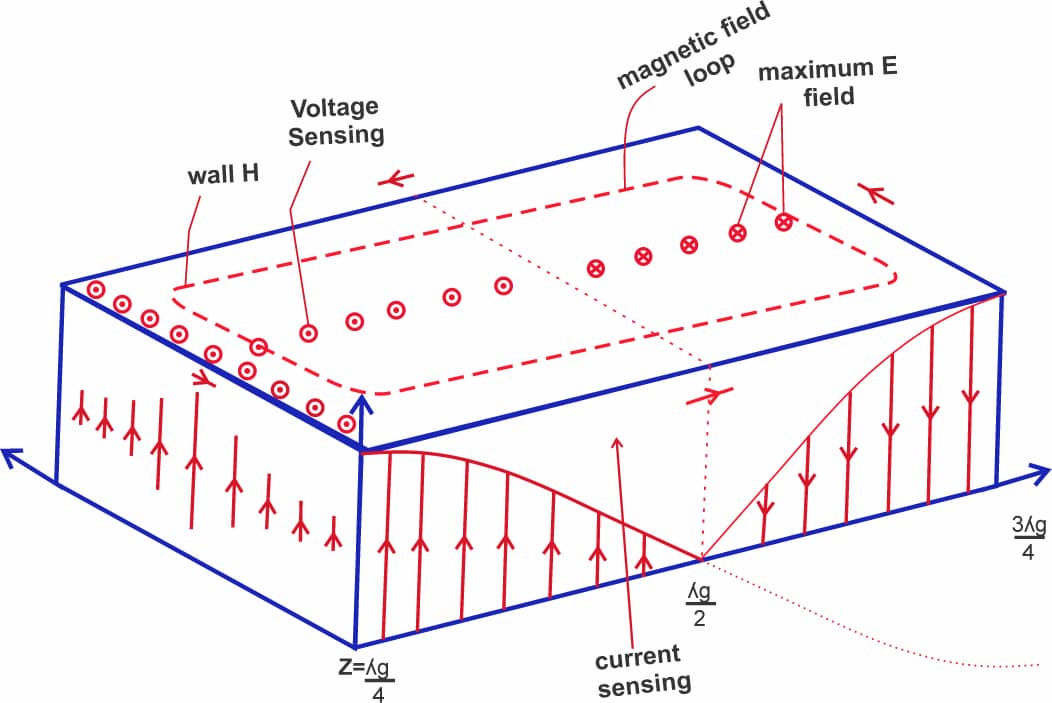
\includegraphics[width=1\linewidth]{./graphics/lecture-image-2.jpg}
\caption{EM WAVE OF A RECTANGULAR WAVE GUIDE SHOWING THE DIFFERENT FIELD}
\end{figure}
$E_{y}$ will have maximum value at   with sinusoidal variation along x as shown by the length of arrows and they all point in the positive y direction for $x = 0$ to $x = a$. Looking from the top, we have the variation shown with $\odot$ and $\otimes$ showing direction of the field looking from top.
 
The size of the circles shows the strength of the field. So if we go side ways the field has sinusoidal decrease, till it gets to zero at the edges.
 
As we move in the z directions, $E_{y}$ has sinusoidal variation in the z direction and the fields are shown in similar manner. Looking from the side we see the illustration corresponding to sinusoidal variation of the fields as shown. 
So we can write down the plane and the side view for the waveguide.
Visualizing the electric field is very simple as we visualize one component of the electric field which is Y oriented. Same thing we can do for the magnetic fields.
\begin{figure}[h]
\centering
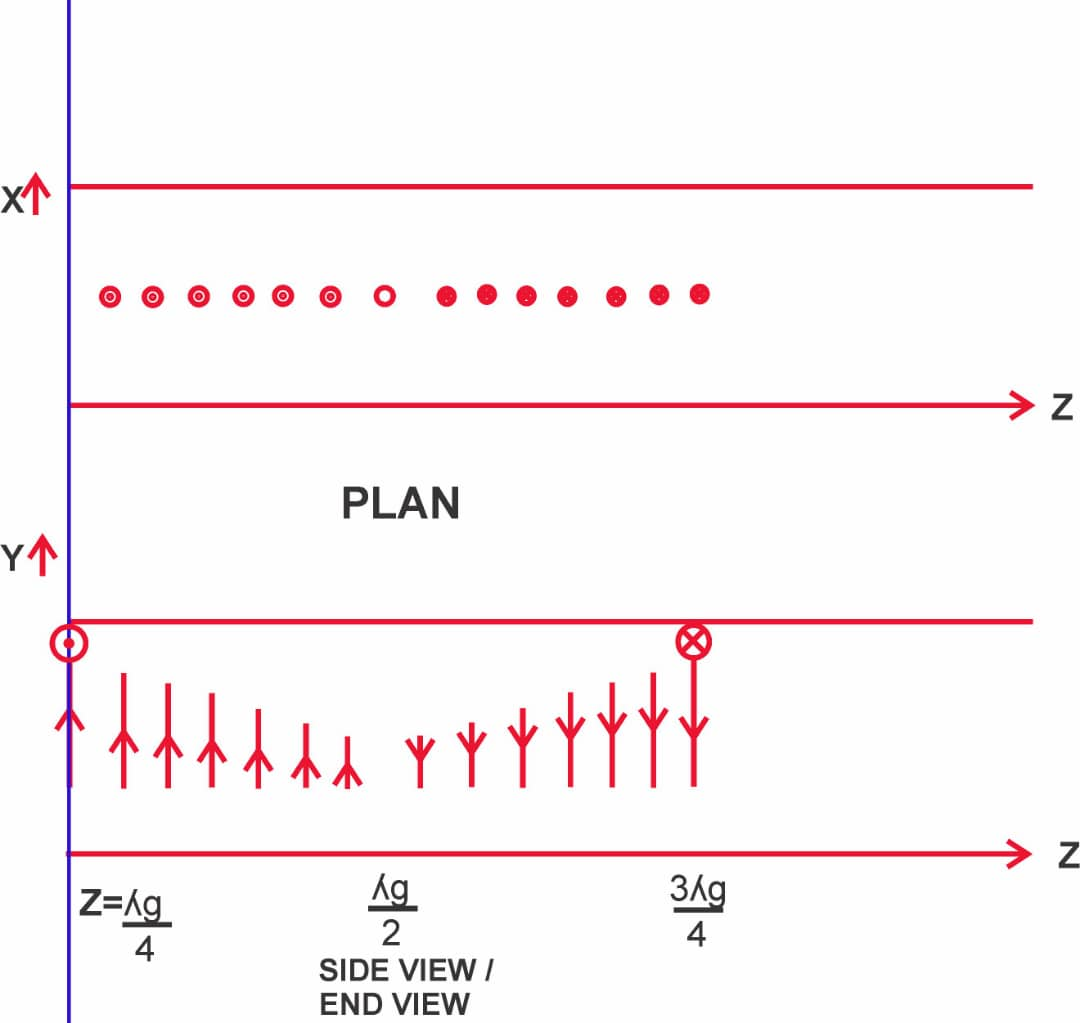
\includegraphics[width=1\linewidth]{./graphics/lecture-image-3.jpg}
\caption{PLAN AND END VIEW OF AN EM WAVE OF A RECTANGULAR WAVE GUIDE}
\end{figure}

As we have seen in the case of parallel plane waveguides, $H_{x}$ have variation same as the electric field by $E_{y}$. $E_{y}$ and $H_{x}$ are maximum at same time and minimum at the same point. But the Z component of magnetic field is shifted by $90^{o}$ or $\frac{\lambda g}{4}$ with respect to the x components. So wherever $H_{x}$ goes to zero, $H_{z}$ is maximum, so it is quadrature in x and z as we see below. We observe that;
\begin{equation}
Re[E_{z}] = C\cos\dfrac{\pi x}{a}\cos\dfrac{2\pi}{\lambda g}z
\end{equation}
\begin{equation}
Re[E_{x}] = B\sin\dfrac{\pi x}{a} \sin\dfrac{2\pi}{\lambda g}z
\end{equation}
So where $H_{x}$ is maximum along Z i.e Z = $\frac{\lambda g}{4}$, $H_{x}$ is minimum.
The magnetic field lines are shown above with arrows designated 1, 2, 3 and 4. Carefully observe $H_{x}$ and $H_{z}$ maximum and where they occur. So because magnetic field must close on itself, 1, 2, 3, 4 must form a loop as shown above.
The variation of the magnetic field in the Y-direction is zero. Hence $H_{x}$ and $H_{z}$ are constant the Y direction. So in the plan view it appears as shown 
\begin{figure}[h]
\centering
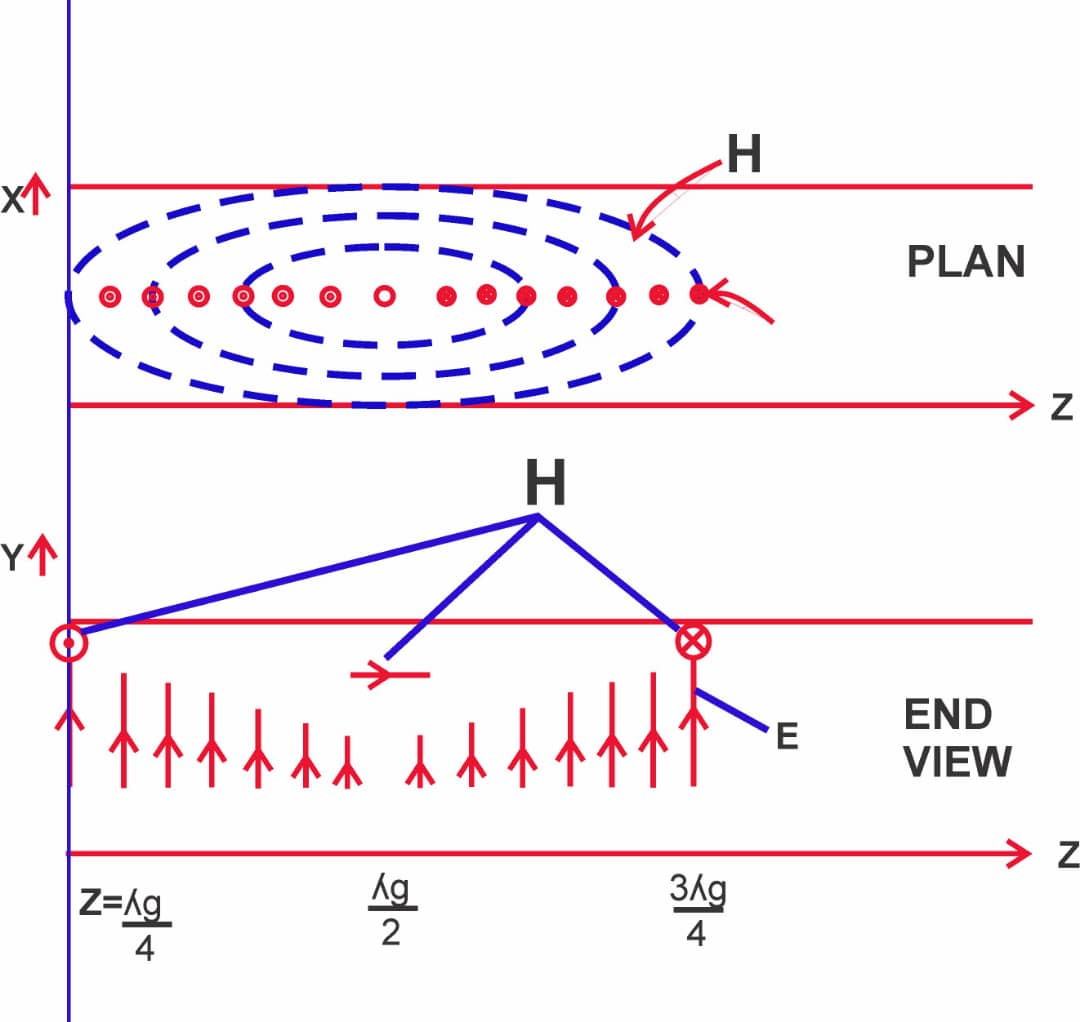
\includegraphics[width=1\linewidth]{./graphics/image-1.jpg}
\caption{PLAN AND END VIEW OF AN EM WAVE OF A RECTANGULAR WAVE GUIDE(SHOWING THE FIELDS)}
\end{figure}

with appropriate direction so that E x H gives the direction of propagation of Z. From the end view, from Z = $\dfrac{\lambda g}{4}$ we have the magnetic field on the side wall coming towards us and at Z = $\dfrac{\lambda g}{2}$ , only $H_{z}$ is represented at 
Z = $\frac{3\lambda g}{4}$. We have $H_{x}$ going in the direction of $\otimes$. So if we visualize this field as a three dimensional structure, the electric fields looks like rods of various various heights or various diameters, where diameters or the heights of the
rod represent the the strength of the electric field and the magnetic field look likes copies of rolled carpets or transformer stampings. shown below is a clever visualization.
\begin{figure}[h]
\centering
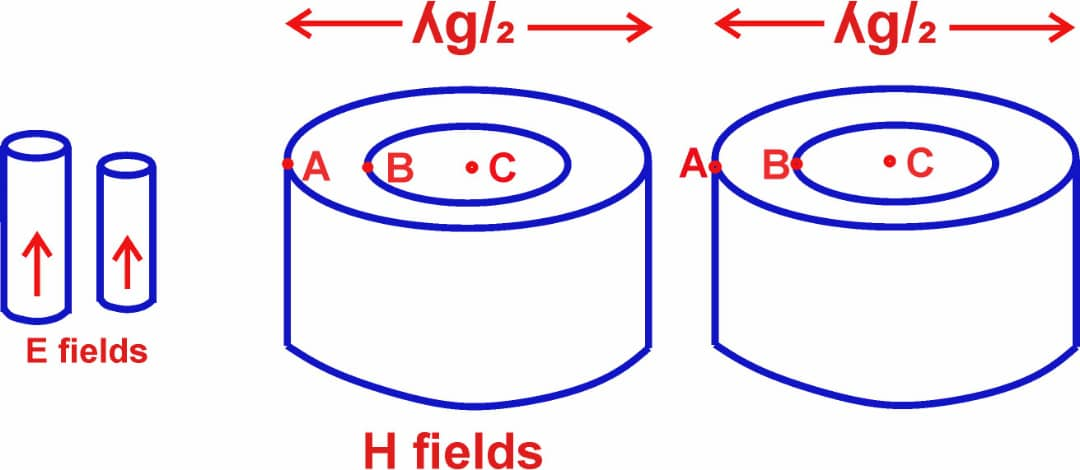
\includegraphics[width=1\linewidth]{./graphics/lecture-image-4.jpg}
\caption{REPRESENTATION OF THE FIELD THREE DIMENSIONAL STRUCTURE}
\end{figure}
	
Now that we get the field visualization at some instant of time, we say let this pattern move with the phase velocity inside the waveguide i.e the pattern starts drifting, so at every location we sometimes see either A,B or C. Now we know that electric field is maximum on the broader wall of the waveguide as mentioned earlier. For the $TE_{10}$ mode, the maximum electric field is along the broad wall along the points   $x = \frac{a}{2}$ as the wave travels in the z direction. The magnetic field would be maximum on wall G and H. It does not vary with Y. So if we have to excite the waveguide by electric fields, with a voltage probe, then the probe must be placed on the line of the broader wall (ie $x = [\dfrac{a}{2}]$ middle point) so that the electric field is excited and that electric field gives excitation corresponding to $TE_{10}$. However, if we have a current probe, we put it on the side walls of G and h which can excite the field distribution shown. Then this would help in exciting $TE_{10}$ Mode inside the waveguide. Same thing is true that if the waveguide was having some modal properties and we want to sense the voltage and current on this waveguide, the voltage probe must be mounted on the broader wall and the current probe must be mounted on the sidewall a and H. This is the way the field inside a rectangular waveguide are detected by using the voltage and current probe, or excited by giving signals to the probe protruding into the waveguides and then excite a field inside a structure.

So this visualization of the field for the dominant mode  which is th the $TE_{10}$ mode is quite useful because it also tells us how the excitation of the field can be achieved by putting voltage and current probes on the wall of the waveguides. Having understood the field distribution in the  $TE_{10}$ mode with electric field more like rod and magnetic field more like rolled carpet or transformer stamping, we can very easily draw the electric and magnetic field for higher order modes. Lets say we want to excite the $TE_{20}$ mode for the rectangular waveguide.

Of course we can write down the field expressions for electric and magnetic fields. Do same thing we did for $TE_{10}$ and visualize the fields. However, once we understood that electric and magnetic field are in specific form, we can stretch our imagination a bit to visualize electric and magnetic field for this higher order mode.

The 2 on $TE_{20}$ mode is telling us that there are two cycles in the X direction and no variation in the Y direction. So the electric field always lie in the Y direction. For the magnetic fields, because the magnetic fields are like stamping or rolled carpets and we are having two sections. Each would have a magnetic loop shown above. The direction of magnetic field will be such that the poynting vector is in the z-direction. In the region between the two magnetic loops, all the fields are essentially going together, so we have two rolled carpets stacked against each others in the waveguide of $TE_{20}$ mode. So once a basic understanding of visualizing fields is developed, it is easy to visualize the fields for higher order modes. The next question we ask is when the fields are excited inside this waveguide, surface current will be induced in the waveguide. Again we come back to $TE_{10}$ mode. We have seen that surface current is related to the tangential component of magnetic fields. So in the figure above, on the top wall, the direction of magnetic field keeps changing, however on the side wall's.The magnetic field direction is always along z direction. Though magnitude is changing, but it is always along the z direction. n x H of side walls, H is in the -y direction i.e going down ward in the y direction
\begin{figure}[h]
\centering
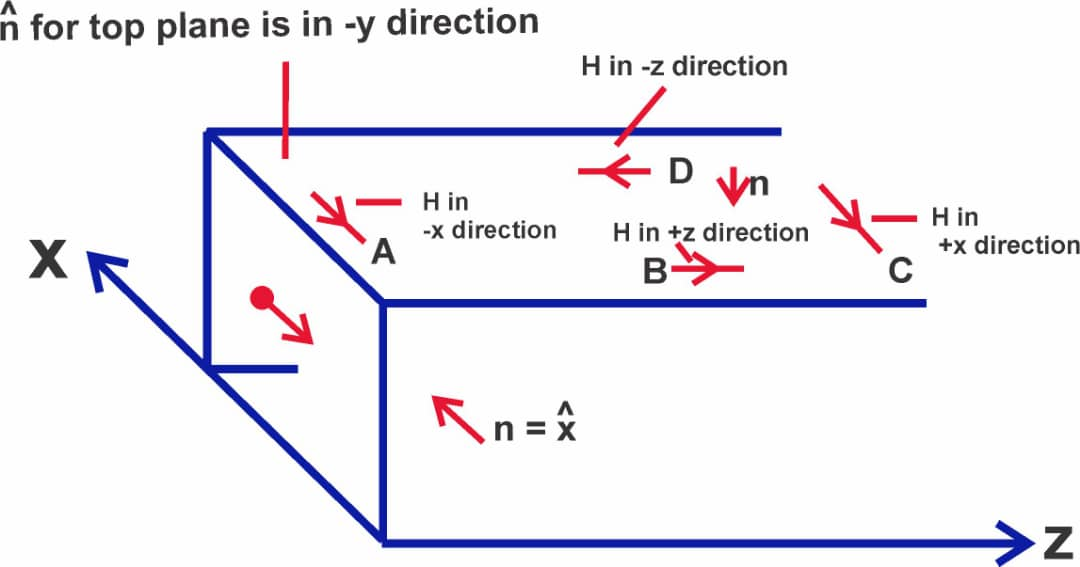
\includegraphics[width=1\linewidth]{./graphics/lecture-image-5.jpg}
\caption{DIRECTION OF THE SURFACE CURRENT AND MAGNETIC FIELD IN A RECTANGULAR WAVEGUIDE}
\end{figure}
\begin{figure}[h]
\centering
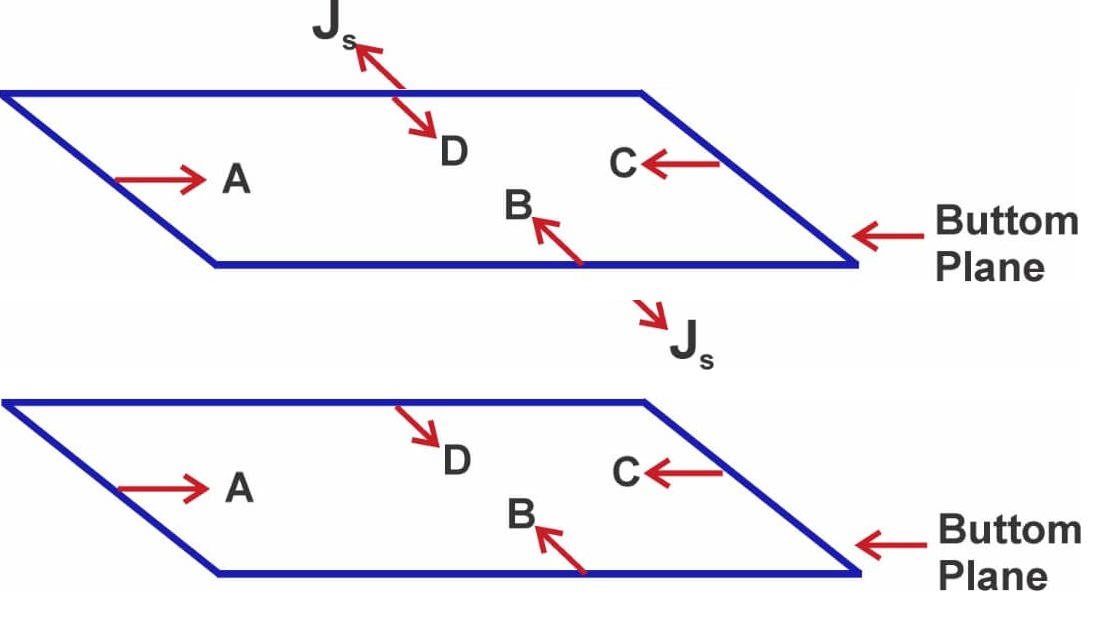
\includegraphics[width=1\linewidth]{./graphics/lecture-image-6.jpg}
\caption{DIRECTION OF THE SURFACE CURRENT AND MAGNETIC FIELD ON THE TOP AND BUTTON PLATE OF A RECTANGULAR WAVE GUIDE}
\end{figure}

On the top plane, At
\begin{equation}
   \hat{n} \times H = -\hat{y} \times (-\hat{x})= -\hat{z}
\end{equation}
\begin{equation}
   \hat{n} \times H = -\hat{y} \times (+\hat{z})= -\hat{x}
\end{equation}
\begin{equation}
    \hat{n} \times H = -\hat{y} \times (+\hat{x})= \hat{z}
\end{equation}
\begin{equation}
    \hat{n} \times H = -\hat{y} \times (-\hat{z})= \hat{z}
\end{equation}
Hence we see the variation of $J_{s}$ as it keeps changing direction in the plane. For right side wall it is in z direction +z and for left side wall it is in -z direction.
Left   
\begin{equation}
n\times H = -\hat{x} \times (-\hat{z})= -\hat{y}
\end{equation}
Right  
\begin{equation}
n \times H = \hat{x} \times (\hat{z}) = \hat{y}
\end{equation}
For the above, the surface current is going in y-direction only upon one face down on the other sign is immaterial here.
	
The bottom plane has the opposite direction for $J_{s}$ corresponding to the top plane as calculated and it is shown above. So looking at the current distribution for all the four walls and combining them together, we have the figure below.
\begin{figure}[h]
\centering
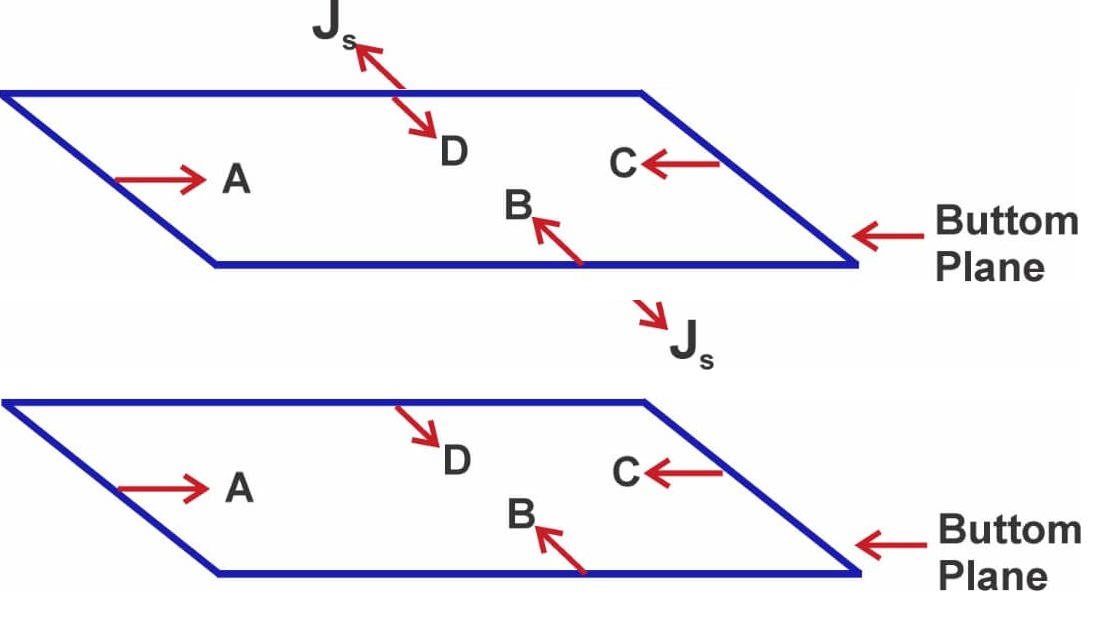
\includegraphics[width=1\linewidth]{./graphics/lecture-image-6.jpg}
\caption{DISTRIBUTION OF CURRENT DENSITY IN A RECTANGULAR WAVE GUIDE}
\end{figure}

So in the figure for the right side wall, the magnetic field was in z-direction and at $\pi$ region $J_{s}$ was in y-direction as we solved above. On the top normal direction is y, so then we have a situation shown where it is as if current is just coming out of the top plane or coming into a point on the top plane or bottom plane depending on the location under consideration. So on the side wall the current does not change as H on the side wall was also constant. It is zero at the center of the top plane, it increases as we get to the side of the top plane, remains constant on the side wall and then decreases till it becomes zero on opposite points to the top wall where H started from. In fact the current is as if it is starting from nowhere it grows and dies down on the opposite to the wall where it started. In the next half cycle, direction of the current will charge and this repeats itself periodically.In one circle the current flows upward that is the charge move downward. In another half cycle, the current flows downward i.e the electrons moves upward. So accumulation of charges takes place between two walls and the charges keep going back and forth and essentially the current flows on the surface of the waveguide. So for every $\frac{\lambda g}{2}$ we have a current island created. It grows and becomes maximum and then decrease to zero on the top plane and bottom plane. It repeats this every $\frac{\lambda g}{2}$. So the current flow is like blooming flower around both sides, with one like a source and other like a sink of current on the opposite top and bottom plane.
	
So this is how the current is going to get induced on the rectangular waveguide. This current helps us to also find out, if we cut the waveguide and allow some slots inside the waveguide, we will see later in antennas that if the current are disrupted, then there is a possibility of getting radiation from the system. So if the current direction in the waveguide is known. them we know where we should cut the slots in the waveguide. So that there is a possibility of radiation. If we cut a slot which does not distort the current flows, as shown in the diagram.

\begin{figure}[h]
\centering
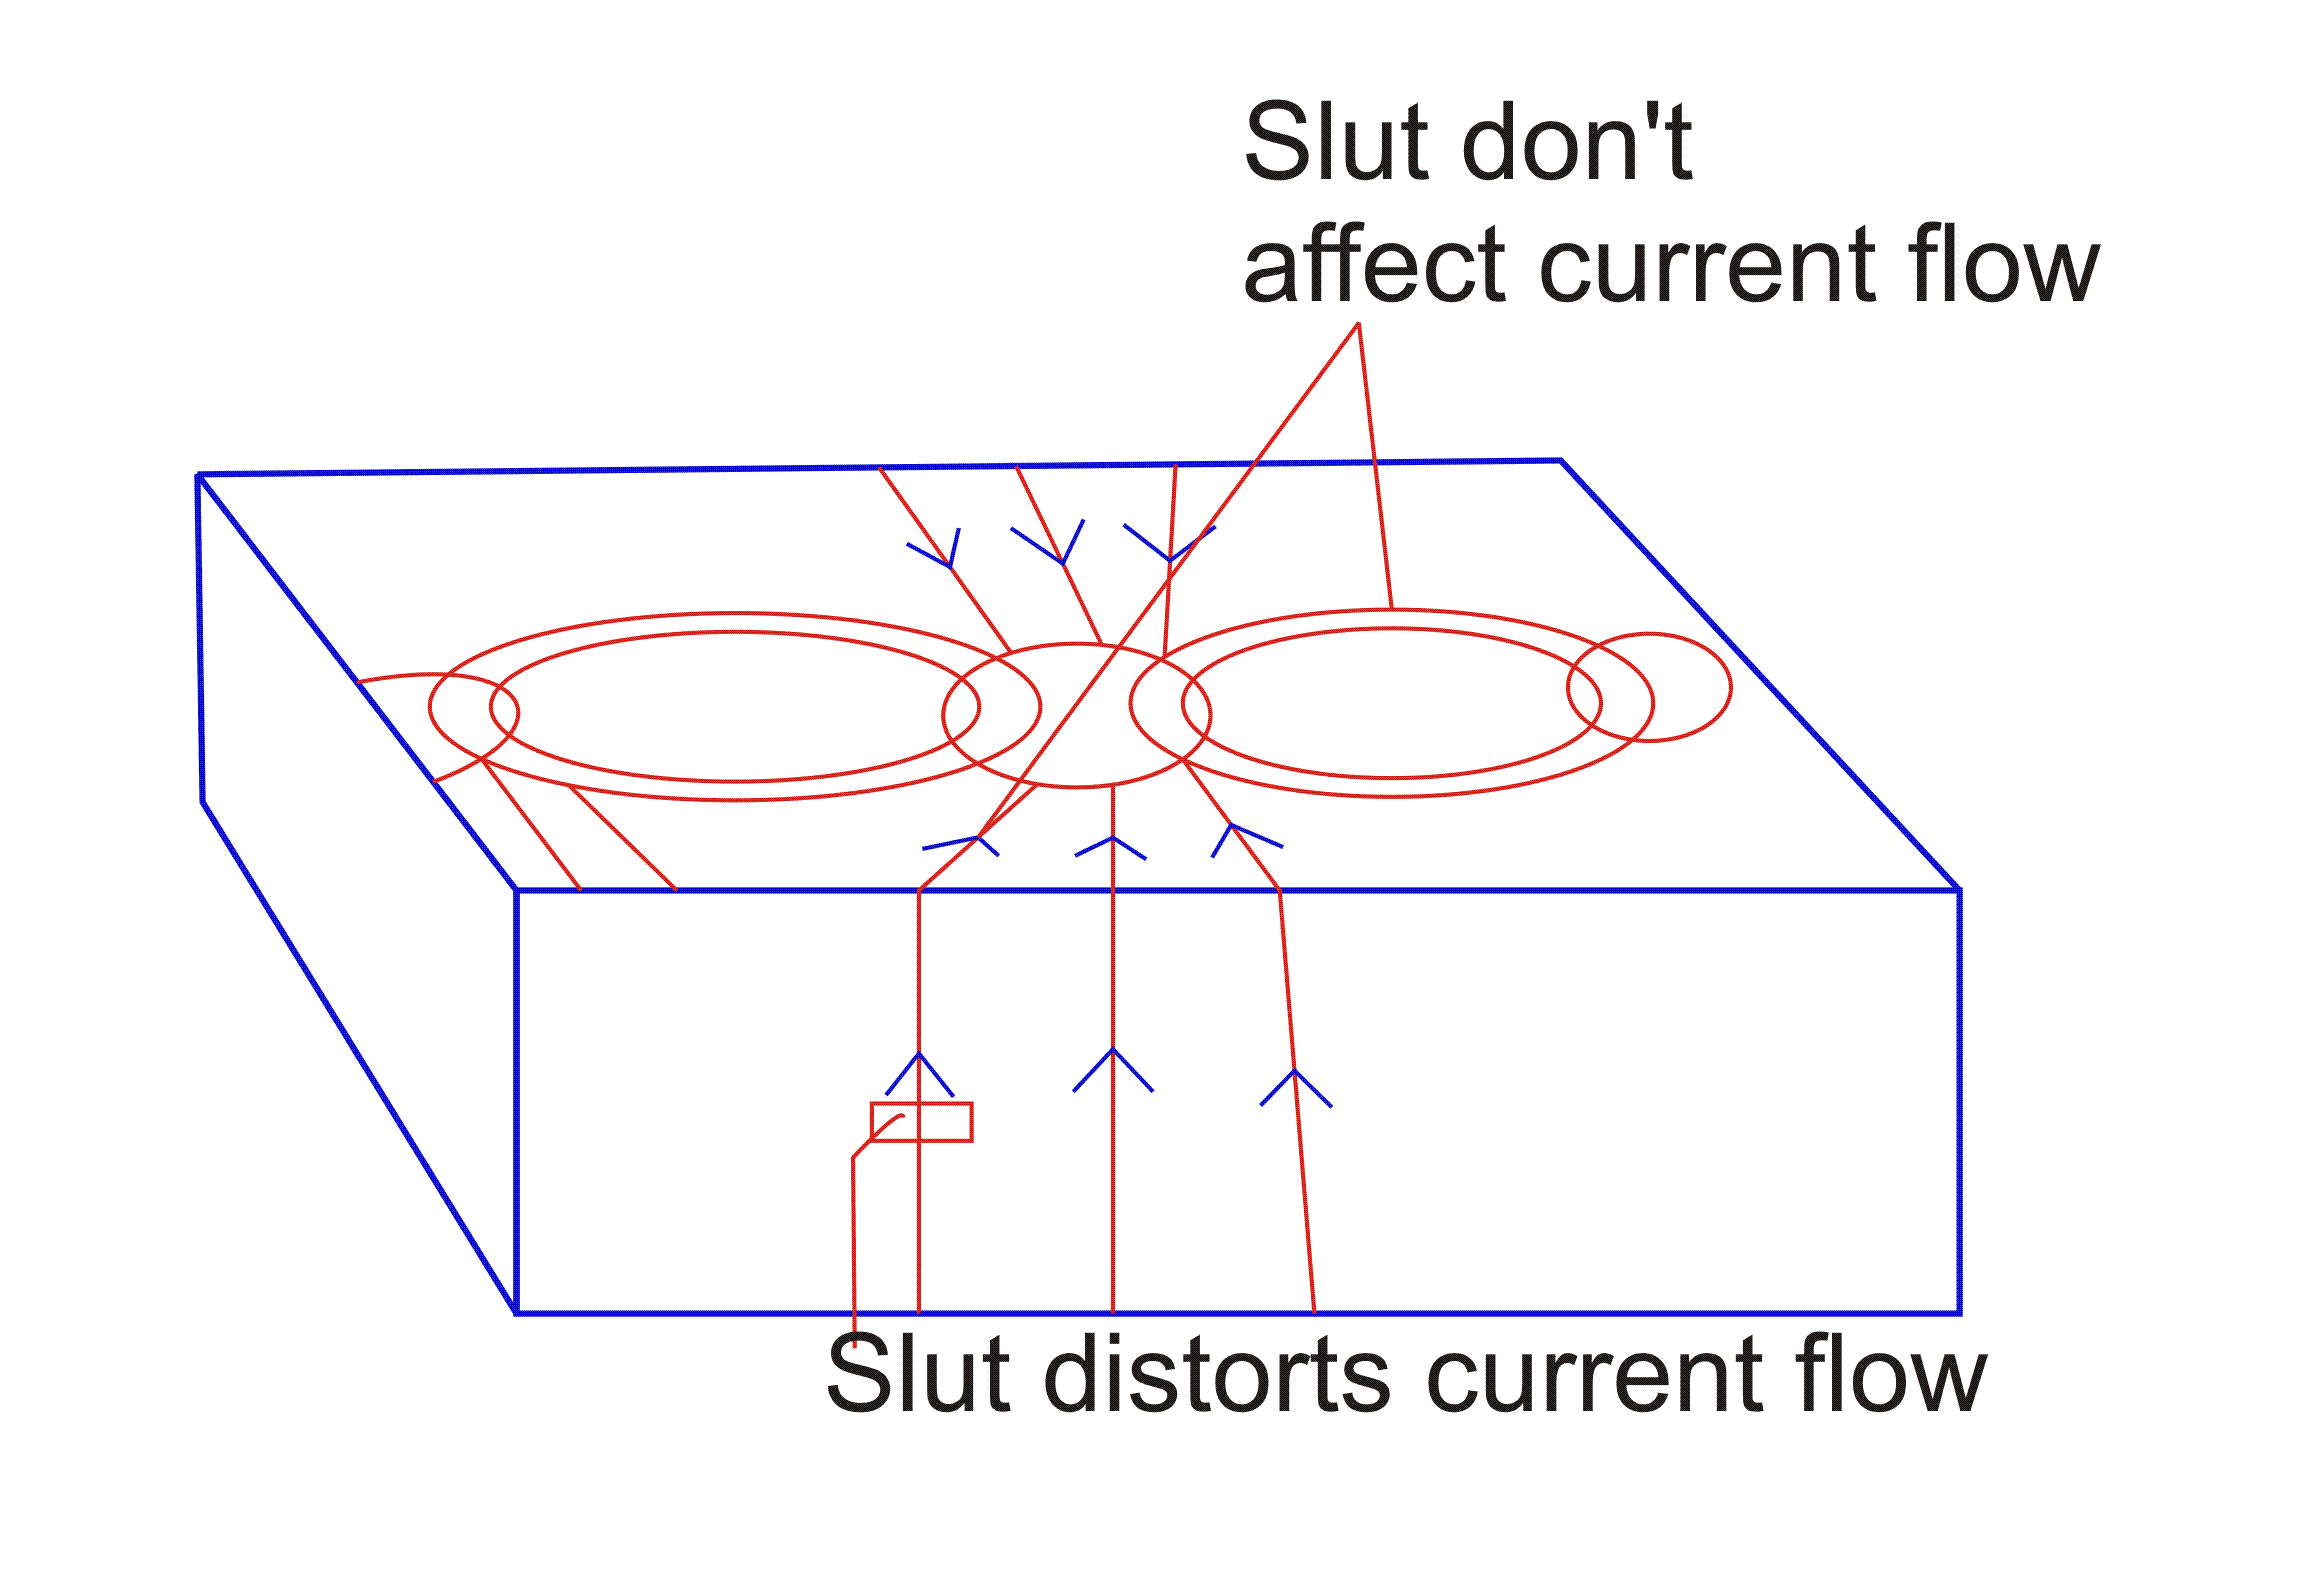
\includegraphics[width=1\linewidth]{./graphics/lecture-image-10.png}
\caption{DIAGRAM SHOWING THE RELATIONSHIP BETWEEN SLOT AND CURRENT FLOW}
\end{figure}
 Because of that there is less possibility of radiation. So if we know the direction of current on this waveguide, we then know were to cut the slots on the waveguide to get radiation.

Another usefulness of finding current direction is if the walls are not ideal conductors, the current flowing will create ohmic losses, that means the power should have been propagated inside the waveguide, part of it will get lost in ohmic heating of the waveguides and this is related to the current distribution on the walls.So the knowledge of current distribution is useful in finding out how the structure can be made to radiate and also how the losses will change if the walls are not ideal conductors.
	
With this, we can go to the next important topic in waveguides i.e the loss calculation in the rectangular waveguide. We have seen that if the structure are not ideal i.e he dielectric filling the the waveguide is not an ideal dielectric, and if the conductor is not ideal conductor, i.e conductivity is not infinite there will always be loss of energy when it propagates through the structure.
Now we try to find out what is the loss per unit length of this waveguide. As we know, it it is measured by a parameter called ATTENUATION CONSTANT.

We have seen in Transmission Line, that if there is a loss in Transmission Line, the variation will be $e^{-\alpha z}$ were $\alpha$ is the attenuation constant. So all the the fields exponentially decays as we travel along the structure. Here we assume that the attenuation constant will cause exponential decay of the fields as they travel. We are interested in finding out the attenuation constant of the conductivity parameter for the walls and the loss in the dielectric is given. However the problem in this case is a little complicated and for this simple reason, if we consider an arbitrary loss in the wall, and arbitrary loss in the dielectric. The modal analysis which we have carried out has to modified now because, the field distribution we earlier assumed we had ideal conductors and ideal dielectric. So in the presence of loss, the electric and magnetic fields are going to get modified, and modification of electric and magnetic fields will change the loss, since the loss is related to current distribution. So essentially we are in a loop that the loss calculation requires the knowledge of electric and  magnetic fields and the electric and magnetic fields depend on the loss.
	
The problems is very complicated, in fact if we went to solve this for arbitrary loss, in the dielectric for arbitrary conductivity of the walls, if assume that the primary function of this waveguide was to transfer energy from one point to the other efficiently, we make every effort to get the losses as minimum as possible.
That means we make a waveguide of a material which has a high conductivity as possible and fill this waveguide with a dielectric as pure as possible. So normally the loss which takes place either in the dielectric filling this waveguide or the finite conductivity of the conducting plane is very very small. Under the assumption, then we can say that as a first order, the fields do not get disturbed significantly because of the losses in the waveguide. What this means is we assume that fields we got for any of the modes are exactly the same as the lossless waveguides even in the presence of this small loss.
So we said that we have a full knowledge of the electric and magnetic fields and once we say that the loop is broken. So from the knowledge of electric and magnetic fields, we can find out what is the current, from there we can find out what is the ohmic losses and then we can calculate attenuation constant. Normally what we will do since attenuation is coming because of the two components viz, loss in the dielectric and then loss in the conducting walls. We separate out these two losses. We say well since the losses are very small, when we calculate dielectric losses, we assume that the waveguide is made of high conductance. When we calculate the conductive losses we assume the waveguide is filled with ideal dielectric. So if we say we have attenuation constant $\alpha$, it consist of two components and two first order approximation, $\alpha$ is the sum of two alphas, $\alpha_{d}$ for dielectric loss and  $\alpha_{c}$ for conductor loss. So $\alpha =  \alpha_{d} +  \alpha_{c}$. When calculating $\alpha_{c}$ we assume  $\alpha_{d} = 0$ and when calculating  $\alpha_{d}$, we assume  $\alpha_{c} = 0$.
	
In calculating  $\alpha_{d}$ we use same approach we used for a Transmission Line. That is we calculate the propagation constant $\beta$ and from the special relation, simply replace the dielectric constant by the dielectric constant of a lossy medium.

\begin{equation}
\beta^{2} = \omega^{2}\mu\epsilon_{l} - (\frac{\pi}{a})^{2}
\end{equation}
for lossy medium. With $\epsilon_{l}$ is for lossy medium, $\beta$ for $TE_{10}$ mode say.
\begin{equation}
\epsilon_{1} = \epsilon_{o}\epsilon_{rl}
\end{equation}
\begin{equation}
\epsilon_{rl} = \epsilon_{r}(1-j\tan\delta)
\end{equation}
Where $\tan\delta$ = loss tangent
We replace $\epsilon_{l}$ by this to have 
\begin{equation}
\beta^{2}_{l} = \omega^{2}\mu\epsilon_{o}\epsilon_{r}(1-j\tan\delta)
\end{equation}
$\tan\delta$ is usually small for low loss dielectric medium.
$$
\beta^{2}_{l} = \omega^{2}\mu\epsilon_{o}\epsilon_{r} - j\omega^{2}\mu\epsilon_{o}\epsilon_{r}\tan\delta$$
$$ = \beta^{2} - j\beta^{2}\tan\delta \equiv \beta^{2} - j\omega^{2}\epsilon_{o}\epsilon_{r}\tan\delta
$$
\begin{align}
\beta_{l} = (\beta^{2} - j\omega\mu\epsilon_{o}\epsilon_{r}\tan\delta)^{\frac{1}{2}} \simeq \beta - \dfrac{j\omega^{2}\mu\epsilon_{o}\epsilon_{r}\tan\delta}{2\beta}
\end{align}
So we have a phase constant $\beta_{l}$ which as a real and imaginary part. The real part is $\beta$. Attenuation constant due to lossy dielectric filling the waveguide
\begin{align}
 \alpha_{d} = \dfrac{\omega^{2}\mu\epsilon_{o}\epsilon_{r}\tan\delta}{2\beta}
\end{align}
Recall in waveguide the variation along z is $e^{-j\beta z}$ so you need imaginary values of $\beta$ to give you attenuation. A real value would give oscillatory terms in $\cos\beta z$ and $\sin\beta z$. $e^{-j}(\dfrac{j\omega^{2} \mu\epsilon_{o}\epsilon_{r}\tan\delta}{2\beta})$
becomes an exponentially decaying term.

Since we know that $\tan\delta = \dfrac{\sigma}{\omega\epsilon_{o}\epsilon_{r}}$, We substitute into $$\alpha_{d} = \dfrac{\omega^{2}\mu\epsilon_{o}\epsilon_{r}\tan\delta}{2\beta}$$ to have 
$$
	\alpha_{d} = \dfrac{\omega^{2}\mu\epsilon_{o}\epsilon_{r}\frac{\sigma}{\omega\epsilon_{o}\epsilon_{r}}}{2\beta} = \dfrac{\omega\mu\sigma}{2\beta}
$$
Given the expression for $\beta$ for the lossless case, for the $TE_{10}$ mode which was related to the cutoff frequency of the mode, 
$$
\alpha_{d} =  \frac{\sigma\eta}{2\sqrt{1-(\frac{fc}{f})^{2}}}
$$
where $\eta$ is the intrinsic impedance in the dielectric.
$$	
\eta =  \sqrt{\frac{\mu_{o}}{\epsilon_{o}\epsilon_{r}}}
$$
For lossless case, 
$$\beta = \sqrt{\omega^{2}\mu\epsilon-(\dfrac{m\pi}{a})^{2}-(\dfrac{n\pi}{b})^{2}}$$
For $TE_{10}$ we had, $$\omega^{2}_{c}\mu\epsilon = (\dfrac{m\pi}{a})^{2}+(\dfrac{n\pi}{b})^{2}$$	
As such $$\beta = \sqrt{\omega^{2}\mu\epsilon-\omega^{2}_{c}\mu\epsilon} = \omega\sqrt{\mu\epsilon}\sqrt{1-(\dfrac{fc}{f})^{2}}$$,	
$$\alpha_{d}=\dfrac{\omega\mu\sigma}{2\beta}= \dfrac{\omega\mu\sigma}{2\omega\sqrt{\mu\epsilon}\sqrt{1-(\dfrac{fc}{f})^{2}}}$$\\
Divide numerator by $\omega\sqrt{\mu\epsilon}$
$$= \dfrac{\sigma\sqrt{\frac{\mu}{\epsilon}}}{2\sqrt{1-(\dfrac{fc}{f})^{2}}}$$\\
$=\dfrac{\sigma\eta}{2\sqrt{1 - (\dfrac{fc}{f})^{2}}}$ where $\eta= \sqrt{\frac{\mu}{\epsilon}}$\\
Therefore $\alpha_{d} = \dfrac{\sigma\eta}{2\sqrt{1 -(\frac{fc}{f})^{2}}}$ and $f_c$ is the cut-off frequency of the mode under consideration.

So knowing the dielectric constant of the medium and assuming the loss tangent is very small, ie the losses in the medium are very small, we can establish the attenuation constant $\alpha_{d}$ due to the finite conductivity of the dielectric medium. We say that for two losses, the attenuation constant is proportional to the conductivity of the medium and we see that $\alpha_{d}$ is related t cut-off frequency.
So when frequency is much larger compared to $f_{c}$, we have $\dfrac{\sigma\eta}{2}$ which is very similar to the case of Transmission Line. We recall that if we take the transverse electromagnetic mode, $\frac{\sigma}{2}(\eta)$ was the attenuation constant for the Transmission Line.
So when we talk about the lossy mediums in the unbound medium, that time we get a loss which was $\alpha = \dfrac{\sigma\eta}{2}$. What happens now however is that in the rectangular waveguide, it also depends upon how far away you are from the cut-off frequency, so if you are very close to cut-off frequency, $\sqrt{1 - (\dfrac{fc}{f})^{2}}$ becomes close to zero.
$\dfrac{\sigma\eta}{2\sqrt{1-(\dfrac{fc}{f})^{2}}}$ becomes very large and the dielectric loss $\alpha_{d}$ becomes very large. So now the dielectric loss is a function of frequency which otherwise was not a function of frequency. In the transverse electromagnetic mode,  $\alpha_{d}$ only depended on the conductivity. So $\alpha_{d}$ is proportional to the conductivity of the dielectric $\sigma$, It also depends on how far away you are from the cut-off frequency of a particular mode. As you go closer to the cut-off frequency of a particular mode. As you go closer to the cut-off frequency of the mode, your dielectric loss increases. So by using this we can calculate one component of the attenuation constant and that is the dielectric attenuation constant $\alpha_{d}$.

The second component we want to calculate now is due to finite conductivity of the boundary. this calculation is not as straightforward as this we have just done. Since fields are now inside the waveguide. Simply modifying the propagation constant, but we do not know now how to put this medium as a lossy medium. If the losses are going to take place in the walls. So what we have to do is to go from the first principle and calculate the attenuation constant using first principles. What this means is that if there is a loss in the medium, the $E$ and $H$ of the fields vary as a function of $z$ ie $ {\hat{E}}, {\hat{H}} \ \sim\ e^{-\alpha z}$ where $\alpha$ is the attenuation constant. So the power which is proportional to $|{\hat{E}}|^{2}$ or $|{\hat{H}}|^{2}$ since power is ${\hat{E}}\times={\hat{H}}$. So power density is the power which the waveguide carriers, i.e $\omega\sim e^{-2\alpha z}$ ie varies as $e^{-2\alpha z}$. We can differentiate $\omega$ power with respect to z to get $$\dfrac{dw}{dz}\sim-2\alpha e^{-2\alpha z} = -2\alpha\omega$$ So that $\alpha$ the attenuation constant in general. If we calculate $$\alpha = \dfrac{-\frac{dw}{dz}}{2w}$$ $$w = -2\exp^{-2\alpha z}$$ $$\frac{dw}{dz} = -2\omega_{o} e^{-2\alpha z} = -2\alpha w$$. $$\alpha = \dfrac{-\frac{dw}{dz}}{2w}$$ Physically -$\frac{dw}{dz}$ stands for the rate at which power decrease in the direction $z$ or in the direction of the wave propagation. W is the total power carried by the structure. Now that the attenuation constant can be calculated by two quantities i.e power loss per unit length $(-\dfrac{dw}{dz})$  along the waveguide, divided by two times the power carried by the waveguide.

$\alpha = \dfrac{\textnormal{power decrease / unit length}}{2\times \textnormal{Total power carried by the waveguide}}$
\paragraph{Calculating for attenuating constant:}
Now to calculate the attenuation constant, we require two quantities to be calculated viz power loss per unit length and the total power carried by the waveguide. So if we go to the rectangular waveguide, we have to calculate two things. These is E and H for the waveguide and surface current that will flow in all the four walls. So surface current will give us the loss, and we can calculate it per unit length i.e what is the power loss in the waveguide. Calculating $E\times H$ will give the poynting vector and integrating over the cross sectional  area of the waveguide gives the total power flowing inside the waveguide. So $w = \int\frac{Re}{2}(\bar{E}\times\bar{H^*})={da} = \int \frac{1}{2}Re(\bar{E}\times {H}^*).{da}$ gives the total power flowing in  the waveguide. Once we know the surface current $I_{s}$ on these walls, then we see that power loss per unit area is given by half surface resistance multiplied by $|J_{s}|^{2}$. So knowing the surface current, we can calculate the loss per unit area and since the height of the waveguide is known, we can calculate the loss per unit length of the waveguide. Once we know these two quantities, using the relation $\alpha = -\dfrac{\frac{dw}{dz}}{2w}$, we can calculate the attenuation constant of this waveguide due to finite conductivity of the walls.

In the next lecture, by using the basic definition of the attenuation constant, we will derive the attenuation constant for two modes. One is for a parallel plane waveguide in the TEM mode, i.e the simplest mode just to get a feel of how to calculate this quantity. Then we would go to the calculation of the attenuation constant for a rectangular waveguide for $TE_{10}$ mode. 
% \chapter{wave guide}
In this lecture we will talk about attenuation constant which was studied in the last lecture. In practice, the material with which the waveguide is made, is not an ideal conductor. So, we have ohmic losses in the walls  of the wave guide and also the dielectric which is filling the waveguide may not be an ideal dielectric, and because of that, we may have dielectric losses in the dielectric.


Last time, we saw that the attenuation constant due to two {2} components \textbf{(i) the finite conductivity of the walls and (ii) the finite conductivity of the dielectric filling the waveguide}, which are treated independently. So we calculate the attenuation constants due to each of these components and then we say the total attenuation constant is the sum of the 2 attenuation constants under the assumption that the losses are very small in a good waveguide.

The last time, we calculated attenuation constant due to dielectric material introducing the concept of complex permitivity. So in the dispersion relation, if we replace the dielectric constant by the complex dielectric constant for the medium, then separating the real and imaginary parts, we can get the attenuation constants due to the dielectric losses.

We then develop a frame work for calculating the dielectric constant due to the finite conductivity of the walls and the waveguide.

In this lecture,we will look at two (2) cases of Parallel Plane Waveguide in \textbf{TEM mode} and the other rectangular waveguide \textbf{$\boldsymbol{TE_{10}}$ mode}.

\section{Attenuation Constant For TEM Mode in Parallel Plane Waveguide}

\begin{figure}[h]
\centering
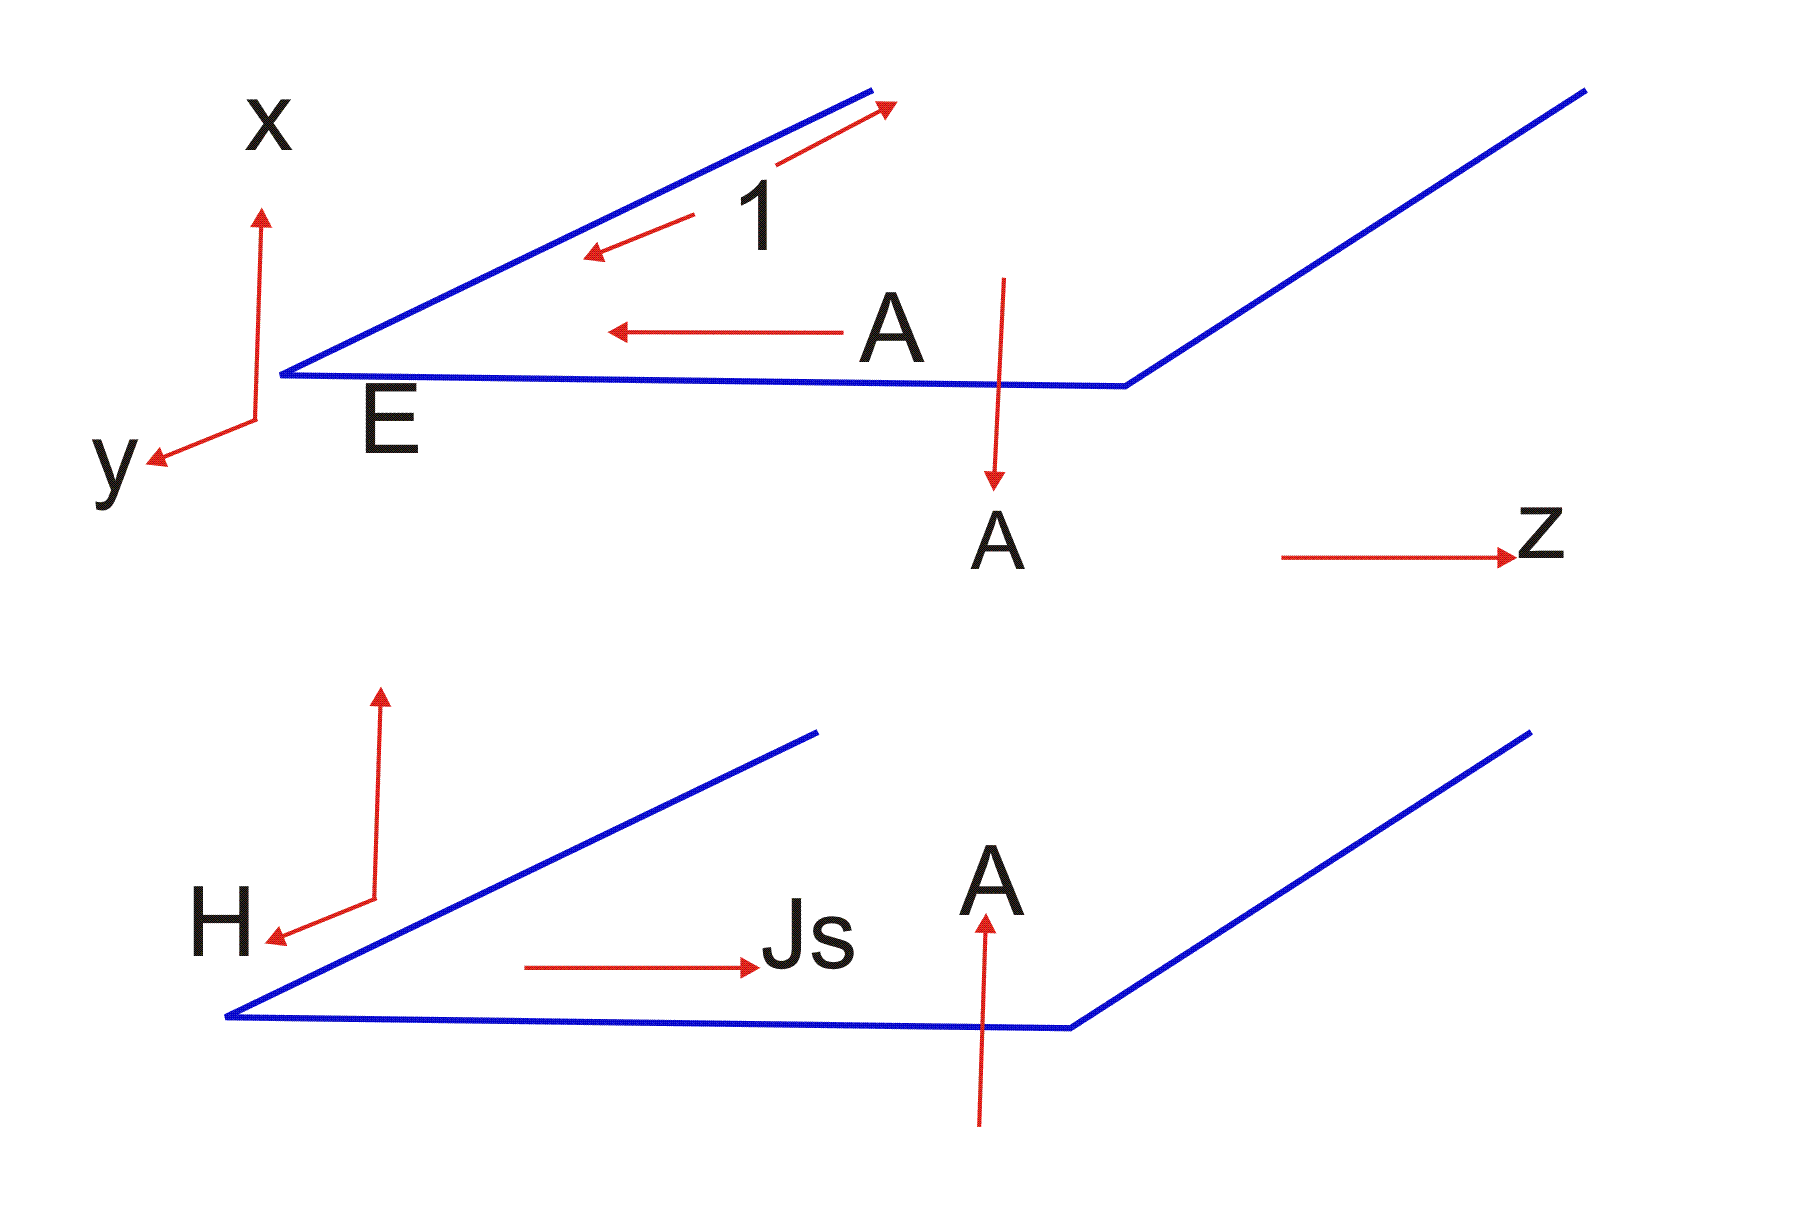
\includegraphics[scale=0.45]{./graphics/lecture2-image-b.png}
\caption{propagation of fields inside a parallel plane waveguide for TEM mode}
\end{figure}

For the calculation of  attenuation constant $\alpha_c$   for TEM in a parallel waveguide to be done, solving for $\alpha_c$  will give us some feel of when we use structures like coaxial cables, parallel wire lines and how the losses are actually calculated. We have seen the calculation of the losses from the knowledge of resistance and conductance in transmission line. However, we ask a question. How do we know the resistance and conductance in this line, s essentially starting from the fields, we can calculate how the losses are going to take place in this conducting surfaces.

Now, let us consider a parallel plane waveguide with wave propagating in the z direction.
%\begin{figure}[h]
%	\centering
%	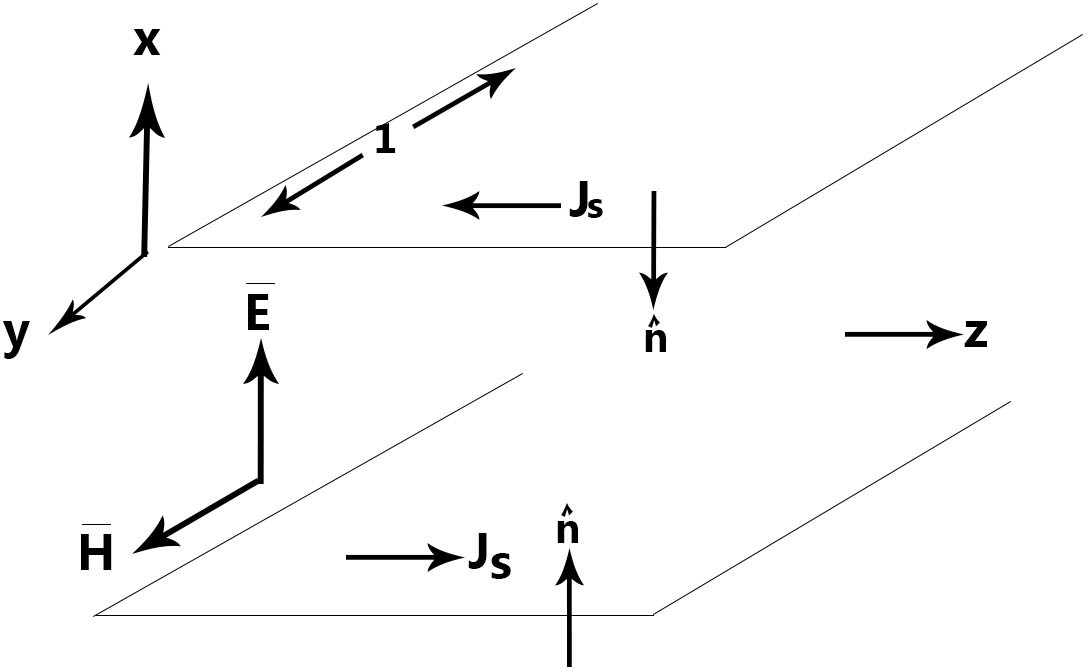
\includegraphics[height=5cm]{411}
%	\vspace{-20pt}
%	\caption{propagation of fields inside a parallel plane waveguide for TEM mode}
%\end{figure}
\begin{figure}[h]
\centering
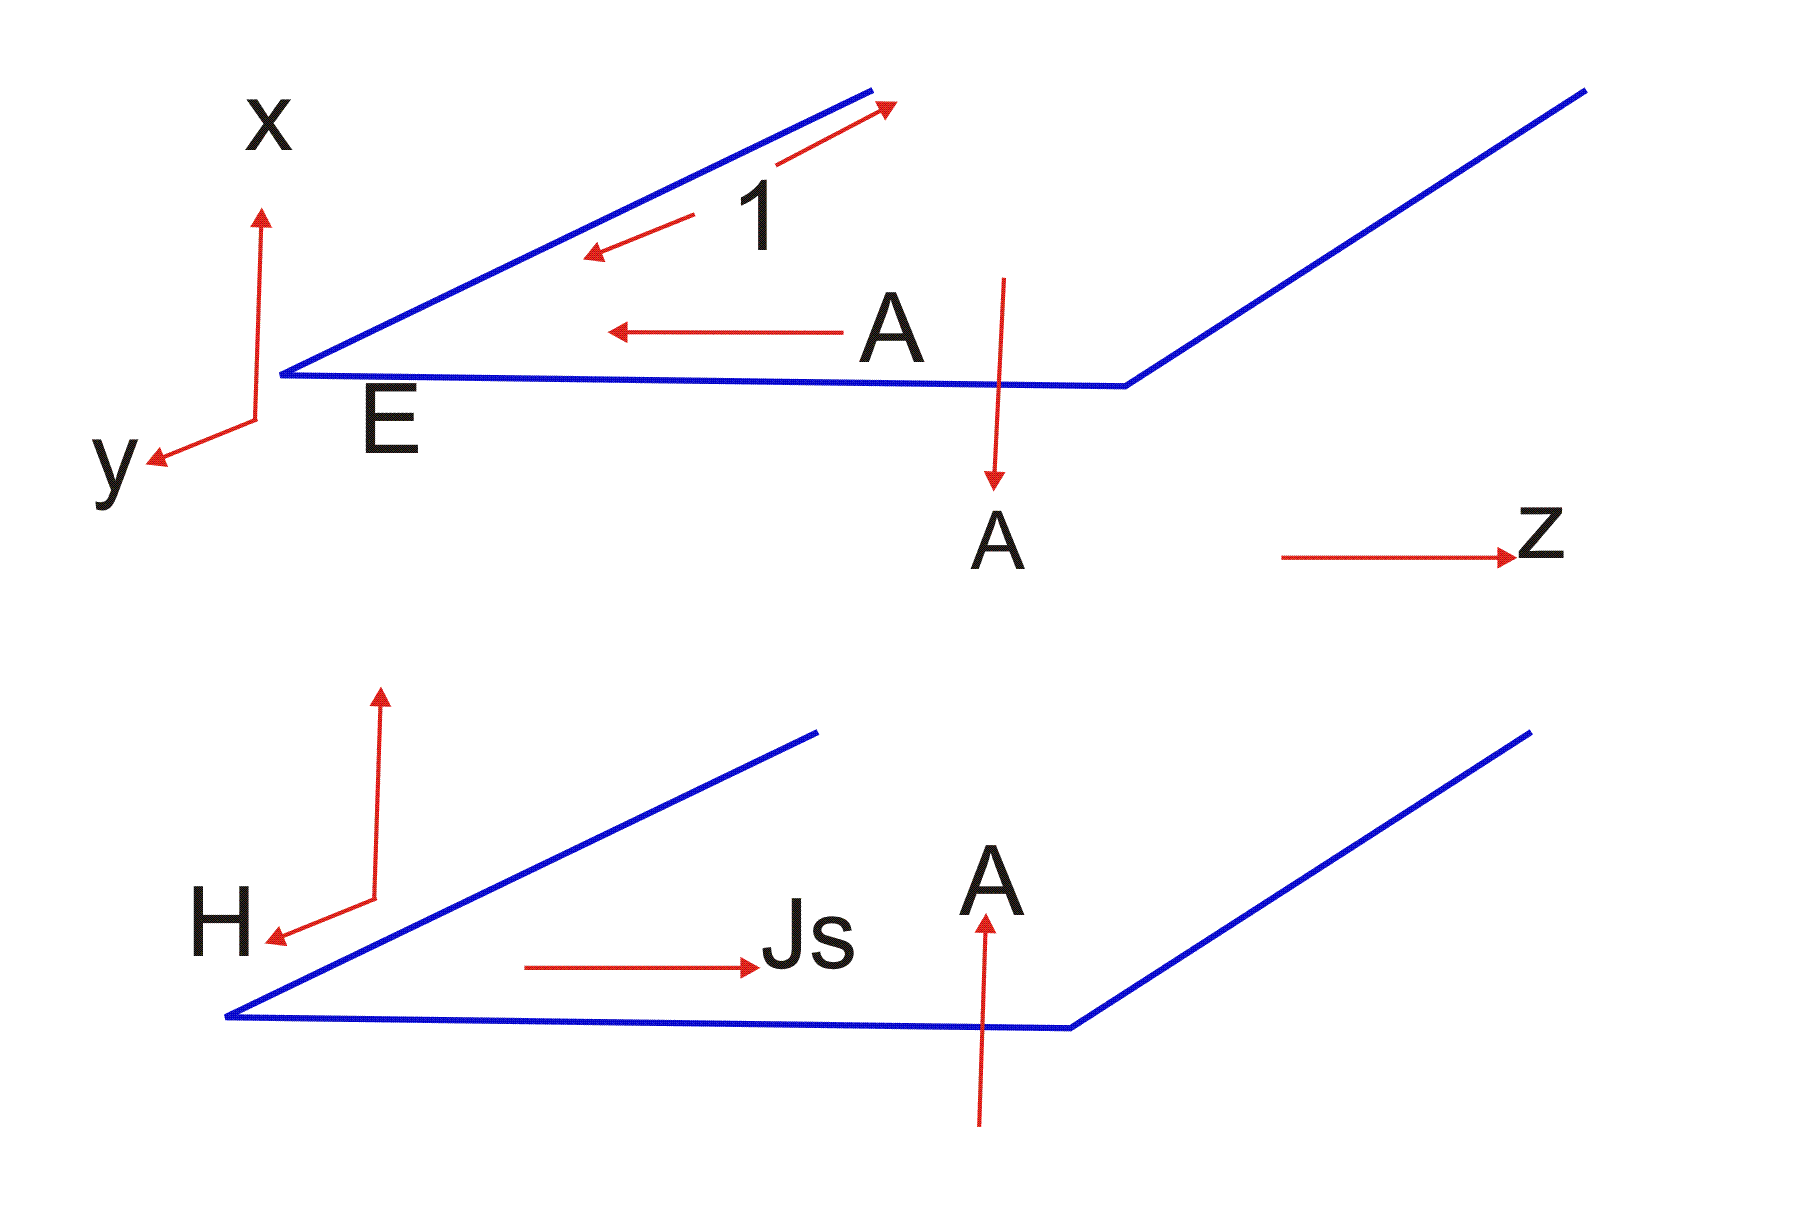
\includegraphics[scale=0.45]{./graphics/lecture2-image-b.png}
\caption{propagation of fields inside a parallel plane waveguide for TEM mode}
\end{figure}
For this case, we say $\overline{E}$ is in the x direction and $\overline{H}$  in the y direction for the coordinate axis. For this mode, the ratio of the $\overline{E}$ and  $\overline{H}$ fields is equal to the intrinsic impedance of the medium filling the waveguide so we have a relation between $\overline{E}$ and  $\overline{H}$

Parallel Plane wave guide $\frac{\overline{E}}{\overline{H}} = \eta $ intrinsic impedance of the medium in the waveguide.

If we express the electric field $\overline{E}$ as some amplitude $E_0$, so that
\begin{equation}
\overline{E} = E_0 e^{-j\beta }\hat{x}
\end{equation}
\begin{equation}
\overline{H} = \frac{E_0}{\eta} e^{-j\beta z}\hat{y}
\end{equation}
Since the waveguide is infinite in the y direction, if we go by the relation
\begin{center}
$\alpha = \frac{\text{power decrease per unit length}}{\text{2 $\times$ total power carried by the waveguide}}$	
\end{center}

to find out the total power carried by the waveguide, then the power will be infinite since the cross section of the waveguide is infinite, y tends to $\infty$. The losses will be infinite and we will not get a definite or meaningful answer.

So we define the $\alpha_{c}$ by the unit width of this waveguide. We take a piece of the waveguide which is of unit length in the y direction i.e (1) in the y direction. What is the powerloss in the unit length of the waveguide? What is the power carried by unit width of the waveguide? From there we can calculate the attenuation constant $\alpha_{c}$ of the waveguide. 

Now we have $\overline{H}$ which is not varying as a function of y, it is constant for y, with amplitude $\frac{E_0}{\eta}$. On top and bottom walls, the magnetic field will be in the y direction.\\\\ As we saw last time, the normal to the surface bounding the electromagnetic wave is as shown. Going by $\hat{n}\times\overline{H}=\overline{J_s}$, we have the direction of $\overline{J_s}$ shown by the arrows. The amplitude of $\overline{J_s}$ is exactly the same amplitude with $\frac{E_0}{\eta}(\overline{H})$. Now that we have visualized the fields and currents inside the waveguide, then, those fields are going to move with the phase velocity inside the waveguide in the z direction.

So, all the  quantities, $\overline{E}, \overline{H}$ are going to have a sinusoidal variation as a function of time. If we consider any location on the conducting plane, the fields, $\overline{E}, \overline{H}$ and the current $\overline{J_s}$ are going to vary sinusoidally as a function of time. So, if we take the peak amplitude, $E_0$ and $\frac{E_0}{\eta}$ of ($\overline{E}$ and $\overline{H}$ ) and find out the RMS value of the fields and the RMS value of the surface currents,we can get the average power lost and average power carried by the waveguide. So for unit width of the waveguide,the power carried by the waveguide per unit width is $\frac{Re}{2}(E \times H^*)$ integrated over the cross section of height (a or d) and width of the waveguide = 1. So, let us say the height of the waveguide is given as a, then the power carried by the waveguide per unit width.

\begin{equation}
W=\int_{x=0}^{a}\int_{y=0}^{1} \frac{1}{2}Re{(\overline{E} \times \overline{H})dxdy}	
\end{equation}
$\overline{E}$ is in x direction, $\overline{H}$ is in y direction, so the power flow is in the z direction. $\overline{E} \times \overline{H}^*$ is we take this to be $\overline{E} \times \frac{\overline{E}}{\eta}$. If we consider the dielectric filling the waveguide is an ideal dielectric, $\eta$ is a real quantity. \\
So, essentially,

\begin{center}
$W$ = $\int_{x=0}^{a}\int_{y=0}^{1}\frac{1}{2}Re(E_0 \frac{E_0^*}{\eta})dxdy$

\end{center}
\begin{equation}
= \frac{\left|E_{0}\right|^2}{2\eta}\int_{x=0}^{a}\int_{y=0}^{1}dxdy = \frac{|E_0|^2a}{2\eta}
\end{equation}


This is the total power carried by the TEM mode per unit width of the waveguide. The second quantity we need is the power loss per unit length of the waveguide. As we have seen earlier, when we go to the concept of what we call surface resistance, if we know the conductivity of the boundary, we can calculate the surface resistance. From the surface resistance, we can calculate the power loss per unit area.
\begin{equation}
=\frac{1}{2}R_s|\overline{J_s}|^2 
\end{equation}

So power loss per unit length 
$ =-(\frac{dw}{dz}) $

This is integrated over the area made by length in z direction and breadth im y direction of 1  unit. We make use of length 1 in z i.e unit length. So area is from 0 to 1 in z and 0 to 1 in y. $ \overline{J_s} $ is the same as a magnetic field, its magnitude will be $ \frac{E_0}{\eta} $ and H* will have a sinusoidal variation in time, so per unit length. If we calculate this value and integrate over the unit area 
, that would give the total loss per unit area of the wall. Since there are 2 walls, the total loss will be doubled. For each wall we calculate
power loss per unit length; 
\begin{equation}
-\frac{dw}{dz}= 2 \int_{y=o}^{1} \int_{z=0}^{1}\frac{1}{2}R_s|\overline{J_s}|^2dydz
\end{equation}
Note: The 2 indicates the 2 walls of the waveguide. 

If we recall, the $R_s$ was the real part of the intrinsic impedance of the conducting wall. For the conducting wall,
$$\eta_c = \sqrt{\frac{j\omega\mu}{\sigma}}= \sqrt{\frac{\omega\mu}{2\sigma}}+j\sqrt{\frac{\omega\mu}{2\sigma}}$$

Recall:
\begin{center}
$\sqrt{\frac{\omega\mu}{2\sigma}}=R_s$	
\end{center}
which is the surface resistance. Also,
\begin{center}
$j\sqrt{\frac{\omega\mu}{2\sigma}}=X_s$
\end{center}
which is the Surface Reactance.
\begin{equation}
\eta_c = R_s + X_s.
\end{equation}
We are interested in power loss here, so that we can substitute for $R_s$ in $\frac{dw}{dz}$ equation to have
\begin{center}
$-(\frac{dw}{dz})=\sqrt{\frac{\omega\mu}{2\sigma}}\times\frac{|E_0|^2}{\eta}$
\end{center}
\begin{equation}
W=\frac{|E_0|^2 a}{2\eta}
\end{equation}
This equation is the power loss per unit length of the waveguide. So, we have the quantities which are needed for the  calculation of attenuation constant .
Attenuation constant 
\begin{center}
$$\alpha_c = \frac{\sqrt\frac{\omega\mu}{2 \sigma}\times\frac{|E_0|^2}{\eta}}{2 \times \frac{|E_0|^2 a}{2 \eta}}$$

$$= \frac{2}{a}\sqrt{\frac{\omega\mu}{2\sigma}}=\frac{1}{a}\sqrt{\frac{\omega\mu}{2\sigma}}$$	
\end{center}
Thus, we get the attenuation constant of the parallel plane wave guide as

\begin{equation}
\alpha_c=\frac{1}{a}\sqrt{\frac{\omega\mu}{2\sigma}}
\end{equation}
$\omega$ is the frequency, $a$ is the height of the waveguide, $\mu$ is the permeability of the dielectric, and $\sigma$ is the conductivity of the parallel planes.Somethings can be observed from this equation, 
\begin{enumerate}[(i)]
\item The attenuation constant is inversely proportional to the height of the waveguide. This makes sense, because if we consider the parallel plane waveguide, since magnetic field does not vary as a function of height, no matter the separation of the two planes, the power loss per unit length is the same as it does not change. However, the power carried by the waveguide is affected in that it increases. But the power loss per unit length does not change and it is small. As a result, the attenuation constant reduces with increasing height, a.
\item The attenuation constant is inversely proportional to the conductivity, $\sigma$. That, we understand, because if you have a good conductor, as the conductivity becomes large, the attenuation gets smaller since there will be less loss in the limit, $\sigma$ tends to $\infty$, $\alpha_{c}$ tends to 0. So, a waveguide made of ideal conductor will have 0 attenuation constant. The important thing to note is that attenuation constant $\alpha_{c}$ is a function of frequency $\omega$. As $\omega$ increase, the attenuation constant $\alpha_{c}$ increases.
\item Attenuation constant is directly proportional to frequency, in that, as frequency increases, attenuation constant increases and vice versa. At high frequencies, the loss becomes excessive and signal cannot be fed effectively. In coaxial cables, at low frequencies, the attenuation constant is manageable whereas high frequencies create a low-pass filtering effect smoothening signals because of too much losses. When the same structure is used to carry signal at high frequencies, the loss becomes excessive, so signal cannot be transmitted efficiently from one point to the other. Looking at another angle, suppose we had to send a broadband signal using this structure, i.e. the signal occupies very large bandwidth, the lower end of the frequency spectrum will go efficiently, but the higher end of the spectrum will not go efficient;y. Its amplitude will be reduced.
\end{enumerate}
At low frequencies  the attenuation  constant  is manageable but when we use the same structures to carry signals at high frequency, the  loss becomes excessive and the signal cannot be transmitted  efficiently from one point to the other. We can also see this from another angle, that suppose we need to send a broadband signal using this  structure i.e if the signal occupy very large bandwidth, the lower  end of the frequency  spectrum will go efficiently but the higher end of the frequency spectrum  will not go efficiently.Its amplitude  would be reduced and the wave guiding structure has an effect like that of a LOW PASS FILTER. So the signal is distorted  as if it was pass through a low pass filter. 
Whenever  there is a guiding structure, invariably there is low pass filtering  and a distorted signal I.e there will be blurring  of the sharp edges of the signal in time. Signals get smoothed out because of low pass filtering action caused by lossy behaviour of the waveguide. Conductor loss varies with frequency and so an increase  in frequency will lead to high loss for the same wave guide structure. 

\section{Transverse Electric Mode (TE10)}
Since this is the mode that will propagate inside a rectangular waveguide. Recall for
$TE_{10}$ mode
\begin{center}
$\frac{E_x}{E_z}=0$

$H_y=0$	
\end{center}
$$
E_{x} = E_{z} = H_{y} = 0
$$	
$$
E_{y} = \dfrac{-j\omega\mu a }{\pi} C\sin \dfrac{\pi a}{x} e ^{-j\beta z}
$$
$$
H_{x} = \dfrac{-j\omega a}{\pi} C \sin\dfrac{\pi a}{x}
e^{-j\beta z} 
$$

$$
H_{z} = C\cos \dfrac{\pi x}{a} e^{-j\beta z}
$$


Last time we saw the current distribution because of these fields. Now we use  these fields to calculate power carried by the waveguide, the loss in the four walls of the wave guide and then we calculate the attenuation constant.\\\\ 
From the waveguide shown below

\begin{figure}[H]
\centering
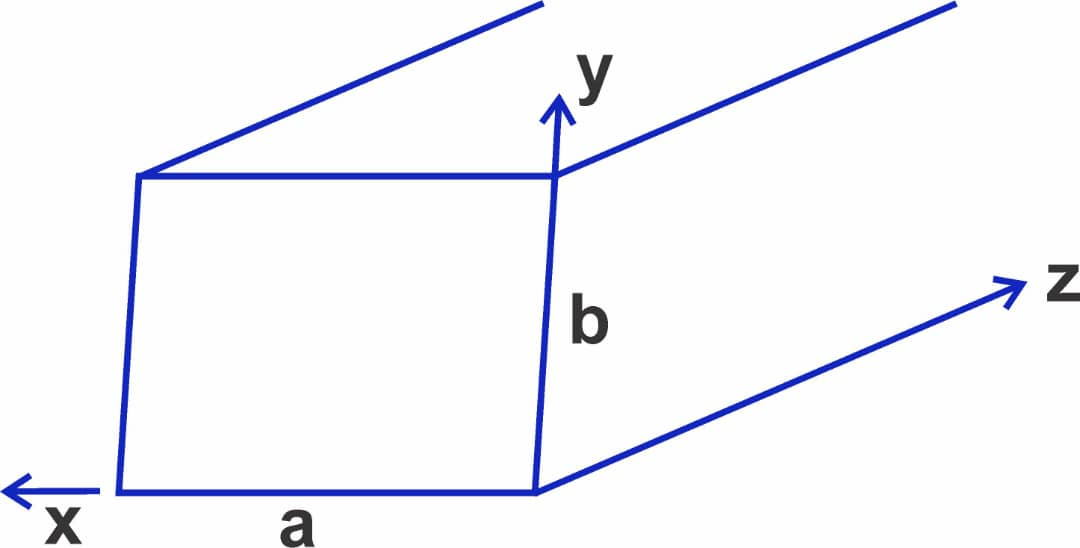
\includegraphics[width=1\linewidth]{./graphics/lecture-image-21.jpg}
\caption{propagation inside a rectangular waveguide2}
\end{figure}


First we calculate the total power since the area of the cross section is known. We take per unit length of the waveguide in the z direction. Calculate the loss per unit length, from same argument, at every location the field is going to sinusoidally as a function of time.
We take the peak value of the magnetic field and just take  the r.m.s value from there and then  we can calculate for the power loss by integrating over the length of the waveguide.
First we take total power or power carried:
\begin{center}
$W= \int_{x=0}^{a}\int_{y=0}^{b}\frac{1}{2}R_e(\overline{E} \times H^*)dxdy$
\end{center}
$E_y$ has -j and $H_x$ has j, $E_y\times H_x^*=$ give -j$\times(-j)=-1$\\
$E_y\times H_2^*$ gives imaginary value. So only $E_y\times H_x^*$ gives real power flow. 

 So,
\begin{center}
$W= \int_{x=0}^{a}\int_{y=0}^{b}\frac{1}{2}R_e(E_yH_x^*(-\hat{z}))+(E_yH_z^*)dxdy$
\end{center}
\begin{center}
$W= \int_{x=0}^{a}\int_{y=0}^{b}\frac{1}{2}\frac{\omega\mu a}{\pi}.\frac{\beta a}{\pi}c^2sin^2(\frac{\pi x}{a})dxdy$
\end{center}
\begin{center}
$=\frac{\omega\mu\beta a^2c^2}{2\pi^2}.b\int_{x=0}^{a}sin^2(\frac{\pi x}{a})dx$
\end{center}
\begin{equation}
=\frac{\omega\mu\beta a^3bc^2}{4\pi^2}
\end{equation}
By knowing the fields for TE10 mode,we can calculate the total  power  carried by the wave guide. Power calculation for the loss in the waveguide is rather tedious  because in the case of parallel plane waveguide,we had only two planes and the current distribution was simple and the current  was moving only in the z direction, so we could integrate very easily. 
For the case of the rectangular waveguide, the current which is flowing on the surface is rather complicated.
We showed last time that it was some kind of blooming and closing flower on the two alternate planes of the rectangular waveguide. 

%\begin{figure}[h]
%	\centering
%	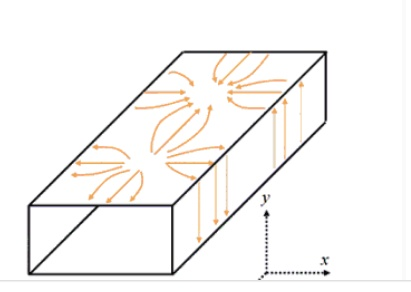
\includegraphics[scale=0.5]{ppw2}
%	\caption{the direction of magnetic and electric fields viewed from the surface of a rectangular waveguide}
%\end{figure}
\begin{figure}[H]
\centering
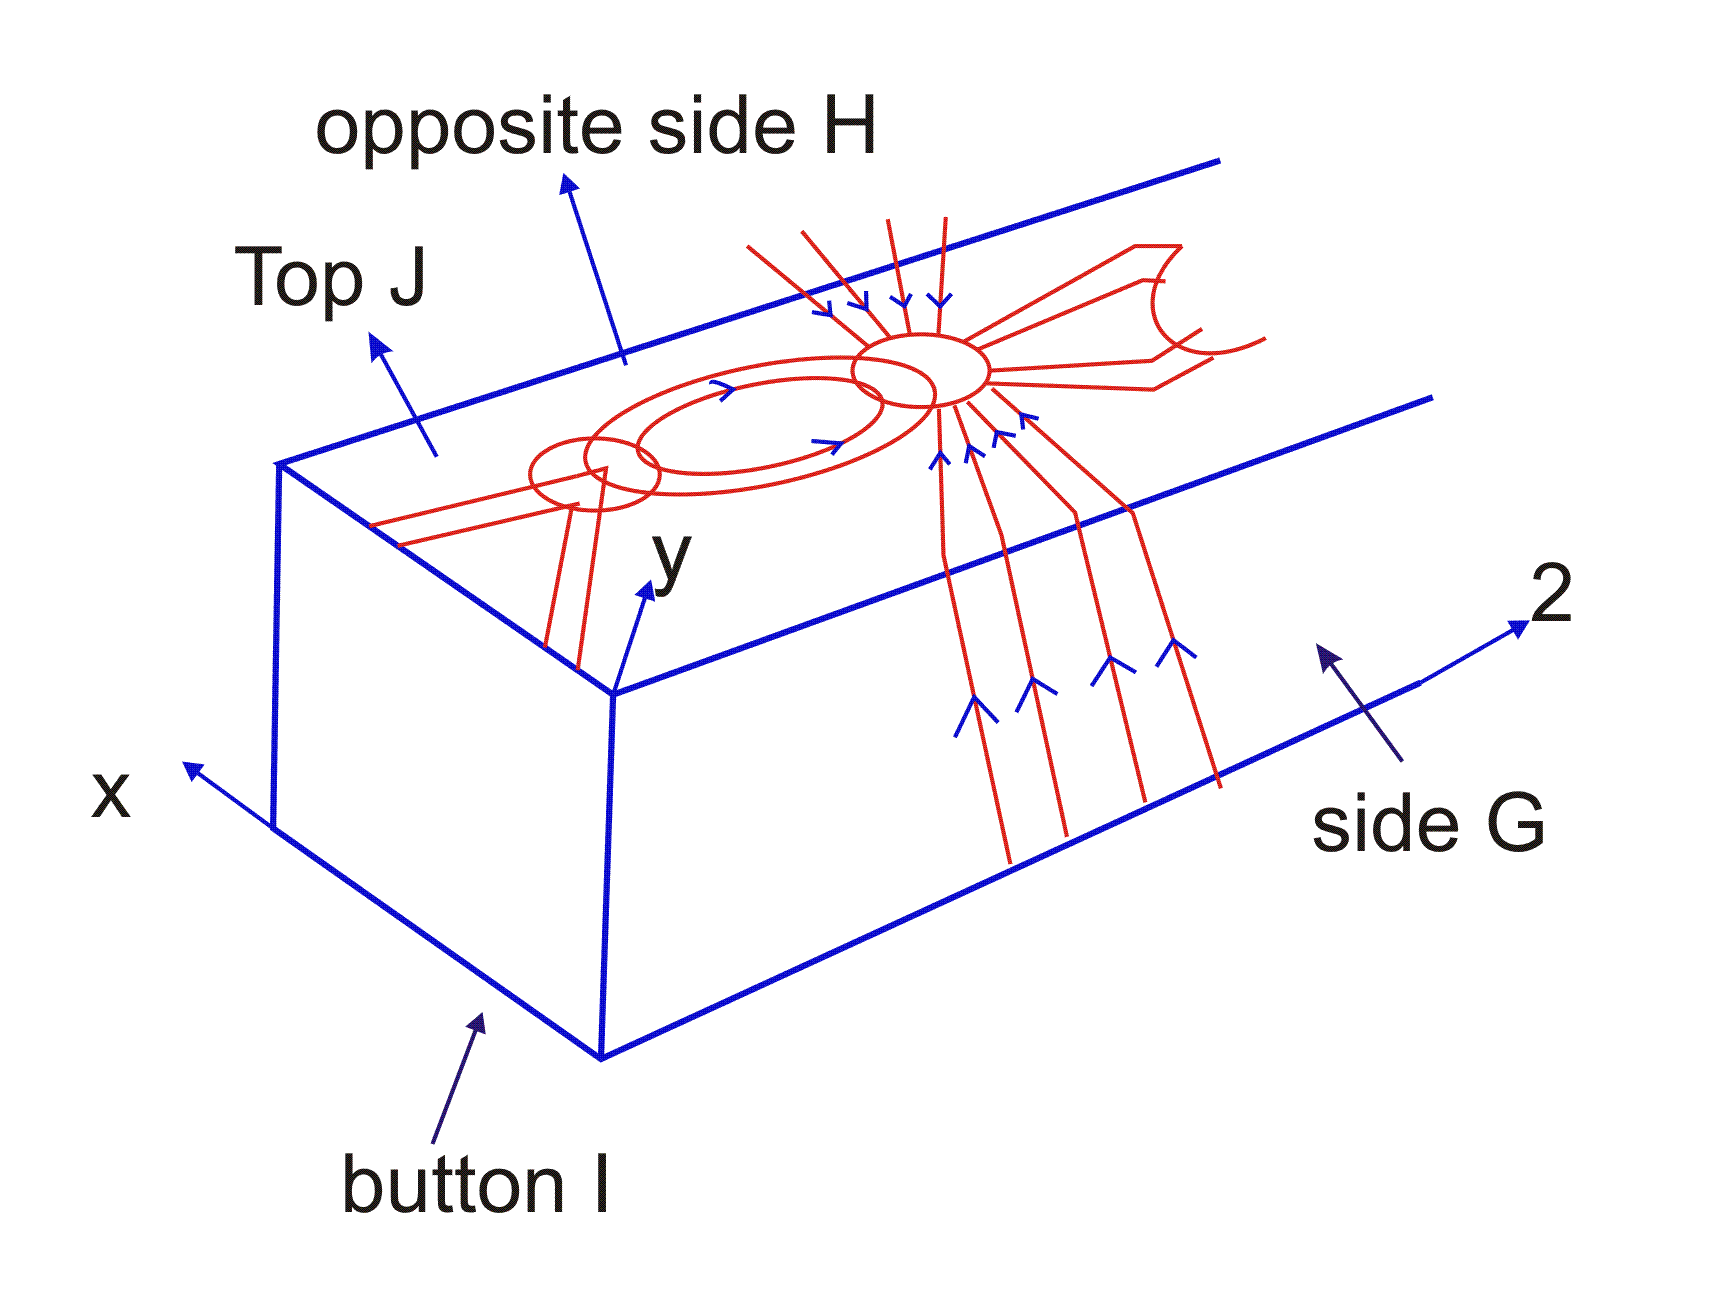
\includegraphics[width=1\linewidth]{./graphics/lecture2-image-a.png}
\caption{the direction of magnetic and electric fields viewed from the surface of a rectangular waveguide}
\end{figure}

On side G, the component of magnetic field was frequency and it varies as a function  of y. So on side G,we have a current that varies only with y. On the top and bottom  surface, we have$H_x$ $H_2$ present. 
$H_x$ is non zero at y=0 and y=b.
Hence on the top, we have current direction in x and z.
On side G and H,we have current that are only y oriented. So,
$$\overline{J_s}|_{x=0} = \overline{J_s}|_{x=a} = H_z|_{x=0 \ or \ x=a}=C$$
from here we can calculate the loss of the waveguide, but we have now the two component of the current.\\ One that is  Z oriented on top and bottom wall and the other x oriented  on top and bottom  wall. So If we are to find the total current  on these walls, we have to have a vector sum of the two currents on the top and bottom surface of the walls of the waveguide. From there we can calculate the total loss  of the waveguide.
First let us calculate the loss for the sidewalls G and H. 
For the side wall $H_2=(cos(\frac{\pi x}{a})e^{j\beta z}$ at x=a gives current inside it which does not vary with y and at x=0 will help give current in G ($\hat{n} \times \overline{H}$) which does not vary with y. Also, $e^{j\beta z}$ gives sinusoidal variation but we are interested in the amplitude,hence instead of writing $ce^{-j\beta z}$ (with x=0 or x=a) we take just C term. So, the current  on the vertical  walls are
\begin{center}
$J_s|_{x=0} = J_s|_{x=a} = H_z|_{x=0 or x=a} = C$	
\end{center}
x=0 represent  wall G and X=a represent wall H. The magnetic field on this side wall
\begin{center}
$H_2=cos(\frac{\pi x}{a}) e^{-j\beta z}$	
\end{center}
does not vary with y. So if we calculate the loss in the two walls per unit length of the waveguide, It is
\begin{equation}
W_L|_{\text{verticalwalls}} = 2\int_{y=0}^{b}\int_{z=0}^{1}\frac{1}{2}R_s|\overline{J_s}|^2dydz
\end{equation}
Recall $\overline{J_s}$ is given by c which we can substitute  in hence to have
\begin{equation}
=R_s|c|^2b
\end{equation}
So calculation  of the loss in the vertical walls is quite simple because we have one component of the surface current which is y oriented. 
However, when we go to the top surface, we have two magnetic field components on the top and bottom surface $H_x$ and $H_z$. So we have to find the total current on this surface and then calculate for the loss for the top and bottom  surfaces. 

\section{HORIZONTAL WALLS} 
$\overline{J_s}$ is a vector  quantity  now as there are two  components in x and z
\begin{center}
$|\overline{J_s}|_{y=0(bottom)} = |\overline{J_s}|_{y=b(top)} = |H|_{y=0}$
$=(|\overline{H}_x|^2 + (|\overline{H}^2 )$
\end{center}
$|\overline{H}|$ is the magnitude  of the total component made up of Hx and Hz.\\\\

Recall
\begin{center}
$\overline{H_x} = \frac{j\beta a}{\pi}Csin(\frac{\pi x}{a})e^{j\beta z}$
\end{center}
\begin{center}
$H_z=Ccos(\frac{\pi x}{a})e^{j\beta z}$
\end{center}
They are not varying as a function of y, so they are the same at y=0 or at y=b i.e at top and bottom  plane which are the two horizontal walls.
\begin{center}
$W_L|_{HOR} = 2\int_{x=0}^{a}\int_{z=0}^{1}\frac{1}{2}R_s(|H_x|^2 + |H_z|^2)dxdz$
\end{center}
\begin{center}
$=\int_{x=0}^{a}\int_{z=0}^{1}R_s ((\frac{\beta a}{\pi})^2C^2 \times sin^2(\frac{\pi x}{a})+ C^2cos^2(\frac{\pi x}{a}))dxdz$	
\end{center}
Solving  this integral we get
\begin{equation}
W_L|_{HOR} = \frac{R_S|c|^2 a}{a}\left(\left(\frac{\beta a}{\pi}\right)^2 +1\right)
\end{equation}
$W_L|_{HOR} + W_L|_{VER}$ =total loss,=losses in horizontal Walls + losses In vertical walls
\begin{center}
$W_L=-\frac{dw}{dz}=W_L|_{VER}+W_L|_{HOR}$	
\end{center}
\begin{center}
$=R_s|C|^2b+\frac{R_s|C|^2a}{2}[(\frac{\beta a}{\pi})^2+1]$	
\end{center}
We can write this in terms of frequency and the cut off frequency of the mode, because we know cut off frequency  is related to the dimension of the waveguide=
\begin{center}
$=R_s|C|^2 (b + \frac{a}{2} + \frac{a}{2}(\frac{\beta a}{\pi})^2)$	
\end{center}
\begin{center}
$ =R_s|C|^2(b+\frac{a}{2}(1+(\frac{\beta a}{\pi})^2)$	
\end{center}
Recall equation for rectangular waveguide:  
\begin{center}
$\beta=\sqrt{{\omega}^2\mu\epsilon-(\frac{m\pi}{a})^2-(\frac{n\pi}{b})^2}$	
\end{center}
\begin{equation}
\beta = \sqrt{\omega^{2} \mu\epsilon-\omega_c^{2} \mu\epsilon}
\end{equation}
with
\begin{center}
$\omega_c^2\mu\epsilon=(\frac{m\pi}{a})^2+(\frac{n\pi}{b})^2$	
\end{center}
For $TE_{10}$, m=1, n=0
\begin{center}
$\omega_c^2\mu\epsilon=(\frac{\pi}{a})^2$,	
\end{center}
\begin{center}
$\beta^2=\omega^2\epsilon-\omega_c^2\epsilon$  or  $\beta^2 + \omega_c^2\mu\epsilon$	
\end{center}
\begin{center}
$= \omega^2\mu\epsilon$	
\end{center}
\begin{center}
$\frac{\beta^2}{\omega_c^2\mu\epsilon}+1=\frac{\omega^2\mu\epsilon}{\omega_c^2\mu\epsilon}=(\frac{f}{f_c})^2$	
\end{center}
\begin{equation}
= 1+ \frac{\beta^2}{\omega_c^2\mu\epsilon}	
\end{equation}
but $\omega_c^2\mu\epsilon=(\frac{\pi^2}{a})$  with  m=1, n=0. From 
\begin{center}
$\omega_c^2\mu\epsilon=(\frac{m\pi}{a})^2 + (\frac{n\pi}{b})^2$	
\end{center}
\begin{center}
$(\frac{f}{f_c})^2= 1+\frac{\beta^2}{(\frac{\pi}{a})^2}$	
\end{center}
\begin{equation}
=1+ (\frac{\beta a}{\pi})^2	
\end{equation}
\begin{center}
$R_s|C|^2 (b+\frac{a}{2}(1+(\frac{\beta a}{\pi})^2)$	
\end{center}
\begin{center}
$=R_s|C|^2(b+\frac{a}{2}(\frac{f}{f_c)}^2)$	
\end{center}
Hence the total loss in the four walls in terms of cut off frequency is
\begin{equation}
W_L=R_s|C|^2[b+\frac{a}{2}(\frac{f}{f_c})^2]	
\end{equation}
So,we know the two things which are needed are: the total power carried by the waveguide which we got and the power loss per unit length of the wave guide. As we saw once we know these two quantities, then we can get attenuation  constant for the waveguide and that will be:
and 
\begin{equation}
W_L=-(\frac{dw}{dz})= R_s|C|^2[b+\frac{a}{2}(\frac{f}{f_c})^2]	
\end{equation}
and
\begin{equation}
W=\frac{\omega\mu\beta a^3bc^2}{4\pi^2}
\end{equation}
\begin{equation}
\alpha_{c}=\frac{-\frac{dw}{dz}}{z\times w}=\frac{R_s|C|^2(b+\frac{a}{2}(\frac{f}{f_c})^2)}{2\times\frac{\omega\mu a^3bc^2}{4\pi^2}}
\end{equation}
Recall:
\begin{center}
$\beta=\sqrt{\omega^2\mu\epsilon-\omega_c^2\mu\epsilon}$	
\end{center}
\begin{center}
$\beta=\omega\sqrt{\mu\epsilon}\sqrt{1-(\frac{f_c}{f})^2}$	
\end{center}
\begin{center}
$\omega^2\mu\epsilon=\frac{\pi^2}{a^2}$	
\end{center}
\begin{center}
$=\frac{R_s[b+\frac{a}{2}(\frac{f}{f_C})^2]}{\omega\mu.\omega\sqrt{\mu\epsilon}\sqrt{1-(\frac{f_c}{f}^2)}\frac{a^2}{\pi^2}ab.\frac{1}{2}}$	
\end{center}
\begin{center}
$=\frac{R_s[b+\frac{a}{2}(\frac{f}{f_c})^2]}{\omega^2\mu\sqrt{\mu\epsilon}\sqrt{1-(\frac{f_c}{f})^2}\frac{1}{\omega^2\mu\epsilon}.\frac{ab}{2}}$	
\end{center}
\begin{center}
$=\frac{R_s[b+\frac{a}{2}(\frac{f}{f_c})^2]}{\frac{\omega^2\mu\sqrt{\mu\epsilon}}{\omega_c^2\mu\epsilon}.\frac{ab}{2}\sqrt{1-(\frac{f_c}{f})^2}}$	
\end{center}
\begin{center}
=$\frac{R_s[b+\frac{a}{2}(\frac{f}{f_c})^2]}{(\frac{f}{f_c})^2\sqrt{\frac{\mu}{\epsilon}}\frac{a}{2}.b\sqrt{1-(\frac{f_c}{f})^2}}$	
\end{center}
\begin{center}
=$\frac{\frac{2}{a}.(\frac{f_c}{f})^2R_s[b+\frac{a}{2}(\frac{f}{f_c})^2]}{\eta.b\sqrt{1-(\frac{f_c}{f})^2}}$	
\end{center}
\begin{center}
=$\frac{R_s[1+\frac{2b}{a}(\frac{f_c}{f})^2]}{\eta b\sqrt{1-(\frac{f_c}{f})^2}}$	
\end{center}
therefore,
$\alpha_{c} for TE_{10}$
\begin{equation}
=\frac{R_s[1+\frac{2b}{a}(\frac{f_c}{f})^2]}{\eta b\sqrt{1-(\frac{f_c}{f})^2}}	
\end{equation}
With $R_s=\sqrt\frac{\omega\mu}{2\sigma}$ in $\alpha_{c}$ expression, it implies  that the higher the frequency, the higher $\alpha_{c}$ and the more the losses. We also know that $\alpha_{c}$  is related to the ratio $\frac{f_c}{f}$. As f tends to $f_C$ becomes very large and when frequency approaches the cut off frequency, there is no propagation of the mode I.e the probation ceases, the power essentially  bounces back and forth between  the two surfaces  and the power is essentially absorbed  in the ohmic losses  of these walls and the attenuation  constant  becomes very large. 
So having  understood these two cases, one was a simple case of parallel plane wave guide in TEM MODE. the other the $TE_{10}$ case which is the mode that is most times  going to propagate inside a rectangular waveguide. We can now calculate the attenuation  constant for any mode.   

We have explained   the philosophy of how attenuated constant calculated inside the waveguide, and using this philosophy, the attenuation  constant can be calculated for any arbitrary mode inside the waveguide.

In summary  the quantity  attenuation  constant is very important  when we use a waveguiding structure In practice. We assume that the waveguiding structure is efficient, that means the losses are very small on this waveguide.
No matter how small these losses are,we always like to get a measure  for that loss so we require the quantity attenuation constant in a parallel  plane waveguide, we saw that the attenuation constant of a waveguide consist of two components:
\begin{enumerate}[(i)]
\item due to dielectric  loss due to finite conductivity of the dielectric  filling the waveguide
\item due to losses arising from finite conductivity of the conducting boundary.
\end{enumerate}
Assuming  that the losses are small for both dielectric  and the conductor, we separately calculate attenuation  constant due to dielectric losses and the conductor  losses and then the total attenuation  constant is the sum of these two attenuation constant.

For calculation of attenuation  constant due to dielectric ,we use the concept of complex permittivity, we replaced the dielectric  constant by complex dielectric  constant in the dispersion relation.By separating the real and imaginary part we get the attention  constant due to dielectric losses. 
For conducting losses, we calculated the total power flow inside the waveguide,and the losses per unit length on the walls of the waveguide. From there we can calculate the attenuation  constant  of  the  waveguide. This essentially complete our discussion on the normal propagating waveguide. 
What we have seen so far in this course is that we started with a wave which was in an unbound medium,and slowly we try to trip the wall into a more and more bound structure.

Reviewing from the Propagation  of plane wave,we started from a wave in an unbound  medium,then we put an interface, we tried to restrict the propagation of wave into semi infinite space,then, we put two planes to trip the wave between  the  planes,to get a structure called a parallel plane waveguide. Then, We restricted the wave from other two directions,so the wave is trapped in a closed pipe which is called a rectangular  waveguide. We can also close from the other two sides I.e we can cut the pipe and close it from both side, then, the wave can be trapped  completely  inside the structure. This structure is essentially  called a resonator which is beyond the scope of this course.from an unbound  medium  to a bound medium  of wave structure explains the way electromagnetic waves are guided in a particular  system. Hence waveguide is an extremely useful device for guiding electromagnetic waves from  one point to another efficiently.

% circular waveguide lectures

% \chapter{Introduction to Bessel Functions}
So far we have treated the rectangular waveguide. In this chapter, we will be discussing the circular waveguide. It is a waveguide with circular cross section in the transverse plane whose wave propagates in the z direction. It has metallic walls like a metal pipe and we will understand how waves propagate in this guide. It is useful for making quality cavity resonator (a structure used to store energy). To solve the problem of how wave propagates, we will use the cylindrical coordinates system.

Now the Helmholtz\footnote{Hermann Ludwig Ferdinand Von Helmholtz (31$|$08$|$1821 - 08$|$09$|$1894) was a German physician and physicist who made significant contributions in several scientific fields.}  wave equation:

$$\nabla^2 \bar{E} + h^2 \bar{E} = 0 $$
$$\nabla^2 \bar{H} + h^2 \bar{H} = 0 $$
becomes complex of form shown below for the $E_z$ component of the electric field.
$$\frac{1}{r} \frac{\partial}{\partial r} (r \frac{\partial E_z}{\partial r}) + \frac{1}{r^2} \frac{\partial^2}{\partial \phi ^2}E_z + h^2 E_z = 0 $$
Recall $h^2 = \omega^2 \mu \epsilon + \gamma^2$. This PDE has a solution called the Bessel function. Therefore in this lecture we will introduce the Bessel function.

\section{Bessel Function}
Consider the second order ordinary differential equation (ODE) shown $$x^2 \frac{d^2 y}{dx^2} + x \frac{dy}{dx} + (x^2 - n^2)y = 0$$
The first solution was proposed by Daniel Bernoulli,\footnote{Daniel Bernoulli (8$|$02$|$1700 - 17$|$03$|$1782) was a Swiss mathematician and physicist and was one of many prominent mathematicians in the Bernoulli family, He is particularly remembered for his applications of mathematics to mechanics, especially fluid mechanics, and for his pioneering work in probability and statistics. His name is commemorated in the Bernoulli's principle, a particular example of the conservation of energy, which describes the mathematics of mechanism underlying the operation of two important technologies of the 20th century: the carburetor and the airplane wing.}
from the famous bernoulli principle and it was for analysis for hanging chain (how it oscillates). We all know a pendulum and therefore we have studied its oscillation with a fixed length of chain. However, there is an oscillation when the length is not fixed and that oscillation was described by Daniel Bernoulli. The second solution was by L. Euler\footnote{Leonard Euler (15$|$04$|$1707 - 18$|$09$|$1783) was a Swiss mathematician, physicist, astronomer, logician, and engineer, who made important and influential discoveries in many branches of mathematics, such as infinitesimal calculus and graph theory, while also making pioneering contributions to several branches such as topology and analytic number theory. He also introduced much of the modern mathematical terminology and notation, particularly for mathematical analysis, such as the notion of a mathematical function.} famous for the Euler formula and it was for the theory of vibrations of circular membrane. For instance, the vibrations on a circular drum. In the end, it was Friedrich Bessel (1784-1846)\footnote{Friedrich Wilhelm Bessel (22$|$7$|$784$\rightarrow$17$|$03$|$1846) German Astronomer, mathematician, physicist and geodesist, influenced by Carl Friedrich Wihhelm Argelander. Laplace function was named after him in his death even if originally discovered by Daniel Bernoulli.} who did a systematic study of this PDE and he proposed the various forms of the solution which forms the basis of the Bessel function and the equation above is called the Bessel equation. Bessel functions are probably the next important functions to sines and cosines. They play a role in electromagnetics, Heat transfer, wave motion, elasticity, scattering problems- where waves are scattered from a cylinder or fluids are scattered in a microfluidic channel with cylindrical dimensions. Essentially, any time there is a cylindrical symmetry, the solution is a Bessel function.

From the above Bessel equation written as;
$$x^2 \frac{d^2 y}{dx^2} + x \frac{dy}{dx} + (x^2 - n^2)y = 0$$ \hspace{0.8cm}\text{\parbox{8cm}{n is a real number which is positive or zero.}}

Let's denote $\frac{d^2 y}{dx^2} \equiv y''$ and $\frac{dy}{dx} \equiv y'$

So 
$$x^2y'' + xy' + (x^2 - n^2)y = 0$$
\begin{equation}
x(xy')' + (x^2 - n^2)y = 0
\label{eqn1}
\end{equation} 
  
For a second order PDE we use the series expansion as the solution of the equation which is the Frobenius method\footnote{Ferdinand George Frobenius  (26$|$10$|$1849 - 03$|$08$|$1971) was a German mathematician, best known for his contributions to the theory of elliptic functions, differential equations, number theory, and to group theory. He is known for the famous determinantal identities, known as Frobenius- Stickelberger formulae, governing elliptic functons, and for developing the theory of biquadratic forms.}.

So the proposed solution is 
$$y(x) = \sum_{k=0}^{\infty}C_k x^{K + \alpha} $$
which is a general power series solution; where $\alpha$ is a constant we introduce to the power of x since the power of x may not necessarily be an integer.

Now let's take the derivative of the proposed solution and substitute for the terms $x(xy')'$ and y in equation \ref{eqn1}.

So
$$y' = \sum_{k=0}^{\infty}C_k (k + \alpha) x^{k + \alpha - 1}$$
$$xy' = \sum_{k=0}^{\infty}C_k (k + \alpha) x^{k + \alpha}$$
$$(xy')' = \sum_{k=0}^{\infty}C_k (k + \alpha)^2 x^{k + \alpha - 1}$$
$$x(xy')' = \sum_{k=0}^{\infty}C_k (k + \alpha)^2 x^{k + \alpha}$$
and substituting in equation \ref{eqn1} gives
$$\sum_{k=0}^{\infty}C_k (k + \alpha)^2 x^{k + \alpha} + (x^2 - n^2)\sum_{k=0}^{\infty}C_k x^{k + \alpha} = 0 $$
  
$$\sum_{k=0}^{\infty}C_k (k + \alpha)^2 x^{k + \alpha} - n^2\sum_{k=0}^{\infty}C_k x^{k + \alpha} + \sum_{k=0}^{\infty}C_k x^{k + \alpha + 2} = 0 $$ 

Now we need to determine the various coefficient $C_k$ and the term $\alpha$ we have introduced. The values will be determined by the equation above. First we note that the equation is true for all powers of x i.e for $x^0, x^1 , x^2$ and so on, hence we have a combination of infinite equations. So let us consider the equation for k=0, we have 
$$ C_0 \alpha^2 x^\alpha - n^2C_0 x^\alpha + C_0 x^{\alpha + 2} =0$$ 
Considering the equation for similar exponent of x gives 
$$ C_0 \alpha^2 x^\alpha - n^2C_0 x^\alpha =0$$
$$ C_0 x^\alpha(\alpha^2 -n^2) =0$$
$\Rightarrow C_0 =0$ or $(\alpha^2 -n^2) =0$ 
$$C_0 =0$$ makes no sense, it means the solution is not going to exist so  $$\alpha^2 -n^2 =0$$ or  $$\alpha =\pm n$$

Next let's consider the coefficients of $$x^{\alpha + 1}$$ for k=1
$$C_1(1 + \alpha)^2 x^{1 + \alpha} - n^2 C_1 x^{1 + \alpha} = 0$$
$$C_1x^{1 + \alpha}[(1 + \alpha)^2 - n^2] =0$$
$$C_1x^{1 + \alpha}[1 + \alpha^2 + 2\alpha - n^2] =0$$
Since $$\alpha^2 = n^2$$ then,
$$C_1x^{1 + \alpha}[1 + 2\alpha] =0;$$ for   $$\alpha =\pm n$$
$$C_1x^{1 + \alpha}[1 + 2(\pm n)] = 0$$ which means $$C_1 = 0$$ since $$n \geqq 0$$
Now let's consider the coefficients of $x^{\alpha + 2}$ for k=2 and k=0.
So $$C_2(2 + \alpha) x^{2 + \alpha} - n^2 C_2x^{2 + \alpha} + C_0x^{2 + \alpha} = 0$$
$$C_0 = C_2[n^2 - (2 + \alpha)^2]$$
We can generalize this relationship since a coefficient is always related to 2 coefficient behind, So we have 
$$C_{k-2} = C_k (n^2 - (k + \alpha)^2)$$
Rewriting the expression
$$C_k = \frac{C_{k-2}}{[n^2 - (k + \alpha)^2]}$$
If k is odd for instance k = 3
$$C_3 = \frac{C_{1}}{n^2 - (3 + \alpha)^2} = 0$$ since $C_1 = 0$ 

Also, $C_5$ will be related to $C_3$ and so the odd coefficient does not exist while for k = even, there are even coefficients.
Let $\alpha = \pm n$

So 
$$C_k = \frac{C_{k-2}}{n^2 - (k + n)^2} = \frac{C_{k-2}}{n^2 - k^2 - n^2 - 2nk}$$
$$ =\frac{(-1) C_{k-2}}{k^2 + 2nk} = \frac{(-1) C_{k-2}}{k(2n + k)}$$ where k is even. 
Let $k =2k$ Such that $k = 1, 2, 3, ...$
Then $$C_{2k} = \frac{(-1) C_{2k-2}}{2k(2n + 2k)} = \frac{(-1) C_{2k-2}}{4k(n + k)}$$
for $k=1$
$$C_2 = \frac{(-1) C_0}{4(n + 1)} = \frac{(-1) C_0}{2^2(n + 1)}$$
for $k = 2$
$$C_4 = \frac{(-1) C_2}{2^2 2(2 + n)}$$ and substituting $C_2$ gives 
$$C_4 = \frac{(-1)^2 C_0}{2^4 2(n + 2)(n + 1)}$$
which seems to show a pattern. Now let's find one more term so we can get a generalized relationship.
For k = 3
$$C_6 = \frac{(-1) C_4}{2^2 3(n + 3)} = \frac{(-1)^3 C_0}{2^6 3!(n + 3)(n + 2)(n + 1)}$$	
So, $$ C_{2k} = \frac{(-1)^k C_0}{2^{2k} k!(n + k)(n + k-1)... (n + 1)}$$	

Let's introduce the Gamma Functions to simplify the expression a little further. Gamma function is basically factorial but unlike factorial which works for only integers, it can be done with any number so it is a generalized factorial function. It is given as 
$$\Gamma(n + 1) = n \Gamma(n)$$
So for $$\Gamma(n + 2)$$ it will be expressed as $$\Gamma(n + 2) = (n + 1)\Gamma(n + 1)$$
Same applies for $$\Gamma(n + 3) = (n + 2)\Gamma(n + 2)$$ which can be further simplified by substituting $\Gamma(n + 2)$
So   $$\Gamma(n + 3) = (n + 2)(n + 1)\Gamma(n + 1)$$ and so on.
Now let's consider
$$C_2 = \frac{(-1)^1 C_0}{2^2(n + 1)}$$
which we can rewrite by substituting $ n + 1 = \frac{\Gamma(n + 1)}{\Gamma(n + 2)}$ as 
$$C_2 = \frac{(-1)^1 C_0 \Gamma(n + 1)}{2^2 \Gamma(n + 2)}$$
So the generalized relationship is 
$$C_{2k} =  \frac{(-1)^k C_0 \Gamma(n + 1)}{2^{2k} k! \Gamma(n + k + 1)}$$
Now we can get the series solution for the Bessel Equation for $\alpha= +n$ as 
\begin{dmath*}
y(x) = C_0 x^n \Gamma(n + 1) \left[\frac{1}{\Gamma(n + 1)} - \frac{1}{\Gamma(n+2)}\left(\frac{x}{2}\right)^2 +\frac{1}{2!\Gamma(n+3)}\left(\frac{x}{2}\right)^4 - \frac{1}{3!\Gamma(n+4)}\left(\frac{x}{2}\right)^6 + ... \right]
\end{dmath*}
Let's define $C_0$ as $$\frac{1}{2^n \Gamma(n + 1)}$$ So that
\begin{dmath*}
y(x) = (\frac{x}{2})^n \left[\frac{1}{\Gamma(n + 1)} - \frac{1}{\Gamma(n+2)}\left(\frac{x}{2}\right)^2 +\frac{1}{2!\Gamma(n+3)}\left(\frac{x}{2}\right)^4 - \frac{1}{3!\Gamma(n+4)}\left(\frac{x}{2}\right)^6 + ... \right]
\end{dmath*}
which is called the Bessel function of the first kind. The function has an order of n and it is represented by the term $J_n(x)$
where J is the Bessel function of first kind, n is the order and x is the variable.

We can rewrite the series solution as 
$$J_n(x) = \sum_{k = 0}^{\infty}\frac{(-1)^k (\frac{x}{2})^{2k + n}}{k! \Gamma(n + k + 1)}$$

From ths expression, let's consider the Bessel function for the zeroth order i.e $n=0$
$$J_0(x) = 1 - \frac{(\frac{x}{2})^2 }{1!} + \frac{(\frac{x}{2})^4 }{(2!)^2} - \frac{(\frac{x}{2})^6 }{(3!)^2} + ...$$

if $\alpha = -n,$ then,
\begin{equation}
J_{-n}(x) = \sum_{k = 0}^{\infty}\frac{(-1)^k (\frac{x}{2})^{2k - n}}{k! \Gamma(-n + k + 1)}
\label{eqn2}
\end{equation}
In general we would expect the solution of the Bessel equation as $$ y(x) = A J_n(x) + B J_{-n} (x)$$

However this solution is only true if n is not an integer. This is because when n is an integer the two terms are linearly dependent, and are related by $ J_{-n}(x) = (-1)^n J_n(x)$ which shows $J_{-n}(x)$ is linearly related to $ J_n(x).$ This can be shown by referring once again to our knowledge of gamma functions.

We know that $$\Gamma(n + 1) = n \Gamma(n)$$
So 	$$\Gamma(n) = \frac{\Gamma(n + 1)}{n} $$
and for negative integer values of n, or zero, $\Gamma(n)$ is infinite. So from equation \ref{eqn2}, the coefficients of the first n terms becomes zero since the gamma function is infinite and the summation starts with $k=n$

So 	$$J_n(x) = \sum_{k = n}^{\infty}\frac{(-1)^k (\frac{x}{2})^{2k - n}}{k! \Gamma(-n + k + 1)}$$
Let's substitute a dummy variable $m= k - n$, so that;
$$J_{-n}(x) = \sum_{m = 0}^{\infty}\frac{(-1)^{m + n} (\frac{x}{2})^{2m + n}}{(m + n)! \Gamma(m + 1)}$$
$$= \sum_{m = 0}^{\infty}\frac{(-1)^{m + n} (\frac{x}{2})^{2m + n}}{(m + n)! m!}$$ where m is an integer\\
comparing the above equation with
$$J_n(x) = \sum_{k = 0}^{\infty}\frac{(-1)^k (\frac{x}{2})^{2k + n}}{(k + n)! k!}$$ where $\Gamma(n + k - 1)=(n + k)!$ for $n= integer$\\
we see that $$J_{-n}(x) = (-1)^n J_n(x)$$
In electromagnetics and optics, n is an integer hence $J_{-n}$ is not an independent solution. Now let's physically examine the function $J_n(x)$ \\
Consider a specific case of $n = \frac{-1}{2}$
\\
So $$J_{-\frac{1}{2}}(x) = \sum_{k = 0}^{\infty}\frac{(-1)^k (\frac{x}{2})^{2k - \frac{1}{2}}}{k! \Gamma( k + \frac{1}{2})}$$
and $$\Gamma( k + \frac{1}{2}) = \frac{(2k - 1)! \sqrt{\pi}}{2^{2k - 1}(k - 1)!}$$
from gamma function relationship where $\Gamma(\frac{1}{2}) = \sqrt{\pi}$.\\
Then
$$J_{-\frac{1}{2}}(x) = \sqrt{\frac{2}{\pi x}}\sum_{k = 0}^{\infty}\frac{(-1)^k x^{2k}}{(2k!)}$$
where $$\cos x =\sum_{k = 0}^{\infty}\frac{(-1)^k x^2k}{(2k!)}$$
So $$J_{-\frac{1}{2}}(x) = \sqrt{\frac{2}{\pi}}\frac{1}{\sqrt{x}}\cos(x)$$
and similarly $$J_{\frac{1}{2}}(x) = \sqrt{\frac{2}{\pi}}\frac{1}{\sqrt{x}}\sin(x)$$

Let's plot the function $ J_{-\frac{1}{2}}(x)$
\begin{figure}[h]
\centering
\includegraphics[width=1\linewidth]{"./graphics/fig 11_1"}
\caption{ Plot of the function $ J_{-\frac{1}{2}}(x)$}
\label{fig:fig-1}
\end{figure}
From the plot, it shows that it is the product of $\frac{1}{\sqrt{x}}$ and $\cos(x)$ which are plotted differently. It is seen that at $x=0$, $\frac{1}{\sqrt{x}}$ goes to infinity and as x increases the $\frac{1}{\sqrt{x}}$ term decreases rapidly as shown. The product of the two functions $(\cos(x)$ and $\frac{1}{\sqrt{x}}$) gives the resulting plot of $J_-{\frac{1}{2}}(x)$. It is seen that the zero points are maintained so $J_-{\frac{1}{2}}(x)$ has the periodicity of $\cos(x)$ but the lobes or amplitude of $J_-{\frac{1}{2}}(x)$ goes on decreasing in value as x increases. Below shows the plot of $J_n(x)$ functions
\begin{figure}[h]
\centering
\includegraphics[width=1\linewidth]{"./graphics/fig 11_2"}
\caption{ Plot of $J_n(x)$ functions}
\label{fig:fig-2}
\end{figure}
Let's consider the Bessel function of the second kind also called the Neumann functions as a second solution to the Bessel equation when n is an integer. It is given by: 
$$Y_n = \frac{\cos(n\pi) J_n(x) - J_{-n}(x)}{\sin(n\pi)}$$
As we have seen from the plot of $J_n(x)$ that every Bessel function of the first kind has a zero value at the centre i.e at $x= 0$ except for $J_-{\frac{1}{2}}(x)$ and $J_0(x)$, where $J_0(x)$ has a peak value at $ x= 0$. Suppose we want to confine the wave such that it is within a single lobe of the function then the solution is of the order of $n =0$ which is $J_0(x)$. On the other hand, the Neumann functions always starts from $-\infty$ at $x=0$ (centre of the waveguide) as shown below
\begin{figure}[H]
\centering
\includegraphics[width=0.7\linewidth]{"./graphics/fig 11_3"}
\caption{ Plot of the Neumann functions}
\label{fig:fig-3}
\end{figure}
In general we will have a solution of the form if n is an integer
$$y(x) = AJ_n(x) + B Y_n(x)$$
In the reality, since $Y_n(0) = -\infty$ makes no physical sense in electromagnetics and electrodynamics so the solution will be 
$$y(x) = AJ_n(x)$$
We will stop here for now and consider the circular waveguide in the next lecture. So this lecture was a general introduction to Bessel functions and as electrical engineers these functions play a very important role in cylindrical symmetry. For the metallic waveguide which we will discuss in the next lecture, it is basically the Bessel function of the first kind which is important. When we consider dielectric waveguides such as the optical fibre which will probably be treated in the optical fabrication courses, we will discuss another function called the Hankel function\footnote{Hermam Hankel(14$|$02$|$1839 - 29$|$08$|$1873) German mathematician, he studied and worked with, among others, Mobius, Riemann Weierstrass and Kronecker.} which is the Bessel function of the third kind. It is basically an exponentially decaying function equivalent to the $e^{-\alpha x}$ kind of function for the dielectric waveguide.
\chapter[Circular Waveguide]{CIRCULAR WAVEGUIDE}
Before we discuss the solution for the circular waveguide let us review what we discussed in the previous lecture and then discuss some important characteristics of the Bessel function when the order n is an integer.

So as we have discussed, for a second order PDE of the form 
\begin{displaymath}
x^2\frac{d^2y}{dx^2} + x\frac{dy}{dx} + (x^2-n^2)y {=} 0
\end{displaymath}
It is called a Bessel equation and one kind of the solution is called the Bessel function of the first kind given as an infinite series
\begin{displaymath}
J_n(x) {=} \sum^\infty_{k=0} \frac{(-1)^k (\frac{x}{2})}{k!\Gamma(n+k+1)}
\end{displaymath}
where n is the order of the solution and $\Gamma(n+k+1){=}(n+k)\Gamma(n+k)$. As we know for any second order PDE there is always two different independent solution and so we have another solution called the Bessel function of second kind or Neumann function given as 
\[Y_n(x) = \frac{\cos(n\pi)J_n(x)-J_{-n}(x)}{\sin(n\pi)} \]
In general the solution of the Bessel equation is \[y(x) = A J_n(x) + B Y_n(x)\]
However \[Y_n(0)=\pm\infty\] which means at the centre of a cylindrical symmetry the electromagnetic fields or power density are infinite at the centre which makes no physical sense. So due to practical reasons the solution of the Bessel function is 
\[y(x) = A J_n(x) \]
There is also the Bessel function of the third kind called the Henkel functions and they play important role in electro magnetics when dealing with dielectric waveguides such as the optical fibre where inside the waveguide we have the Bessel function of the first kind and outside the waveguide we have the Bessel functions of the third kind or Henkel functions.
 
For all electromagnetic problem the order 'n' is always an integer. So we will have forms such as $ J_0(x) $, $ J_1(x) $, $ J_2(x) $, . and so on. Where only $J_0(x)$ has some value at x{=}0 while the rest value of n is zero is 
\[ J_n(0)=0 \; for \; n \neq 0 \]
If we plot these functions, we observe that the behaviour in similar to the sine and cosine function (which means it is periodic) but as x increases the peak value starts decreasing. For instance if we plot $J_0(x)$ as shown it peaks at x=0 and attenuates as x increases.
\begin{figure}[h]
\centering
\includegraphics[width=1\linewidth]{./graphics/fig_1.1}
\caption{}
\label{fig:fig1}
\end{figure}

As we go to higher order functions the behaviour is similar to a sine function. Let's plot the $J_1(x)$ function as shown.
\begin{figure}[h]
\centering
\includegraphics[width=1\linewidth]{./graphics/fig_2.1}
\caption{}
\label{fig:fig2}
\end{figure}

So when looking for the solution for the waveguide there are two constraints involved and they are;
\begin{enumerate}[(i)]
\item What order n do we have for the solution.
\item Which zero point (root) are we considering because the electric field has to get to zero point (root) at the boundary.
\end{enumerate}
 So the first constraint, n tell us how the wave oscillate while the second constraint which we will denote with p, will tell us which zero point we are considering. 

Therefore, a solution would be specified as $J_n^p(x)$ which gives a specific unique solution. For all possible solutions $J_n^p(x_{np})$, there would be a unique value of $x_{np}$, where $J_n^p(x_{np})=0$ given by the table below.
\begin{center}
\begin{tabular}{|c|c c c|}
\hline 
\backslashbox{p}{n} & n=0 & n=1 & n=2 \\ 
\hline 
1&  2.405&  3.832& 5.136 \\ 
2&  5.520&  7.016& 8.417 \\ 
\hline 
\end{tabular} 
\end{center}

The table above as we see tells us where the cut-off frequencies occurs for the circular waveguide. n and p in the circular waveguide is similar to m and n in the rectangular waveguide in a way such that they define the modes and the cut-off frequencies for each mode. We recall from the rectangular waveguide that m shows the number of peaks in the x direction while n shows the number of peaks in the y direction. However, in this case the two arguments n and p show what order of the solution and root of the solution we are considering.
 
 Now let's find the solution of the circular waveguide. Later on we will discuss the derivative of the Bessel function because it is needed in the solution of the waveguide when applying boundary condition.

\section{TM mode in Circular Waveguide}
 So we are considering a hollow metallic pipe of radius a, filled with a dielectric material of $\mu$ and $\epsilon$ as shown.
 
\begin{figure}[h]
\centering
\includegraphics[width=0.7\linewidth]{./graphics/fig_3.1}
\caption{}
\label{fig:fig3}
\end{figure}
For the Helmholtz wave equation 
 \begin{equation}
\bigtriangledown^2\vec{E} + w^2\mu\epsilon\vec{E}=0
\label{eqn12.1}
\end{equation}\
The Laplacian term $\bigtriangledown^2\vec{E}$ has components in the transverse plane and longitudinal. We are still interested in the solution which is of the form of $\vec{E}=\vec{E}_{\bot}e^{-\gamma z}$ where the amplitude $\vec{E}_\bot$ remain in the transverse plane and the wave is propagating in the z direction with propagation constant $\gamma$. 

So we will write equation \ref{eqn12.1} as:
\[\bigtriangledown^2\vec{E}_\perp e^{-\gamma z} + \omega^2 \mu\epsilon E_\perp e^{-\gamma z} = 0\]
where \[\bigtriangledown^2 = \bigtriangledown^2_\perp + \frac{\partial^2}{\partial z^2}\]
So 
\[\bigtriangledown^2_\perp\vec{E}_\perp e^{-\gamma z} + \frac{\partial^2}{\partial z^2}\left(\vec{E}_\perp e^{-\gamma z}\right) + \omega^2\mu\epsilon\vec{E}_\perp e^{-\gamma z} = 0\]
\[\bigtriangledown^2_\perp\vec{E}_\perp e^{-\gamma z} + (\gamma^2)\left(\vec{E}_\perp e^{-\gamma z}\right) + \omega^2\mu\epsilon\vec{E}_\perp e^{-\gamma z} = 0\]
\[\bigtriangledown^2_\perp\vec{E}_\perp e^{-\gamma z} + (\omega^2\mu\epsilon + \gamma^2)\left(\vec{E}_\perp e^{-\gamma z}\right) = 0\]
\begin{equation}
\bigtriangledown^2_\perp\vec{E}_\perp + (\omega^2\mu\epsilon + \gamma^2)\vec{E}_\perp = 0
\label{eqn12.2}
\end{equation}
where $h^2 = \omega^2\mu\epsilon + \gamma^2$. To solve this equation we will use the cylindrical coordinate system. We recall for the rectangular waveguide, we used the Cartesian coordinate system because irrespective of the location we consider along x in the transverse plane the limits along y direction is the same. However for a circular waveguide whose transverse plane is a circle, the limits of y at any location along x changes and so it is preferable to solve the equation using the cylindrical coordinate system because the wave guide has a cylindrical symmetry.
 
The cylindrical coordinate system is defined by $\hat{r}$ and $\hat{\phi}$ in the transverse plane and $\hat{z}$ in the longitudinal direction.
\begin{figure}[h]
\centering
\includegraphics[height=5cm]{./graphics/fig_4.1}
\caption{}
\label{fig:fig4}
\end{figure}
 We will now write equation \ref{eqn12.2} for the cylindrical coordinate as 
 $$
 \frac{1}{r}\frac{\partial}{\partial r}(r\frac{\partial^2\vec{E}_\bot}{\partial r}) + \frac{1}{r^2}\frac{\partial^2\vec{E}_\bot}{\partial\phi^2}+ h^2\vec{E}_\bot = 0 
 $$
 which is the equation which will give the solution of the modes. 

The field components in the circular waveguide are $E_r$, $E_\phi$ and $E_z$ as shown
\begin{figure}[H]
\centering
\includegraphics[height=5cm]{./graphics/fig_5.1}
\caption{}
\label{fig:fig5}
\end{figure}

For the TM mode we know that $H_z=0$ and $E_z$ exists and for the TE mode $E_z=0$ and $H_z$ will exist. Therefore, for the TM mode we should solve for $E_z$ with appropriate boundary conditions and for TE mode, we should solve for $H_z$ with appropriate boundary conditions. 

So for the TM mode we will solve for $E_z$ which should vary in r and $\phi$ and propagates in the z direction as shown $E_z(r,\phi, z)=E_z(r,\phi)e^{-\gamma z}$, where $e^{-\gamma z}$ signifies the field is propagating in the z direction. So from the wave equation for the cylindrical coordinate which we have written, we have;
\begin{equation}
\frac{1}{r}\frac{\partial}{\partial r}(r\frac{\partial E_z}{\partial r}) + \frac{1}{r^2}\frac{\partial^2 E_z}{\partial\phi^2} + h^2 E_z = 0 
\label{eqn12.3}
\end{equation}
And we know r and $\phi$ are orthogonal so whatever variation we have in r is not related to the variations in $\phi$ so we can write $E_z(r, \phi)$ as
$$
E_z(r, \phi) = R(r)\Phi(\phi) 
$$
using separation of variables where $R(r)$ is a function of r only and $\Phi(\phi)$ is a function of $\phi$ only.

So we will write equation \ref{eqn12.3} as 
$$ 
\frac{1}{r}\frac{\partial}{\partial r}(r\frac{\partial(R(r)\Phi(\phi))}{\partial r}) + \frac{1}{r^2}\frac{\partial^2 (R(r)\Phi(\phi)}{\partial \phi^2}) + h^2E_z(r,\phi) = 0
$$
$$
\frac{\Phi(\phi)}{r}\frac{d}{dr}\left(r\frac{dR(r)}{dr}\right) + \frac{R}{r^2}\frac{d^2\Phi(\phi)}{d\phi^2} + h^2 E_z = 0
$$
Divide through by $E_z(r, \phi)=R(r)\Phi(\phi)$ gives 
$$
\frac{1}{rR(r)}\frac{d}{dr}\left(r\frac{dR(r)}{dr}\right) + \frac{1}{r^2\Phi(\phi)}\frac{d^2\Phi(\phi)}{d\phi^2} + h^2 = 0
$$
multiply through by $r^2$
$$
\frac{r}{R(r)}\frac{d}{dr}\left(r\frac{dR(r)}{dr}\right) + \frac{1}{\Phi(\phi)}\frac{d^2\Phi(\phi)}{d\phi^2} + r^2h^2=0
$$
\begin{dmath}
\underbrace{\frac{r}{R(r)}\frac{d}{dr}\left(r\frac{dR(r)}{dr}\right)	+ r^2 h}_{function \; of\; r \; only} 
+ \underbrace{\frac{1}{\Phi(\phi)}\frac{d^2\Phi(\phi)}{d\phi^2}}_{function \; of \; \phi \; only} = 0 
\label{eqn12.4} 
\end{dmath}
which is true for any value of r and $\phi$. The above equation can only be true if each function is a constant and lets denote the constant as $-n^2$ for the function of $\phi$ only ie. 
\begin{equation}
\frac{1}{\Phi(\phi)}\frac{d^2\Phi(\phi)}{d\phi^2}=-n^2 \; \; => \;\; \frac{d^2\Phi(\phi)}{d\phi^2} + n^2\Phi(\phi) = 0
\label{eqn12.5}
\end{equation}
And so $\frac{r}{R(r)}\frac{d}{dr}(r\frac{dR(r)}{dr}) + r^2h$ has to be $+n^2$ so that equation \ref{eqn12.4} holds, hence;
$$
\underbrace{\frac{r}{R(r)}\frac{d}{dr}\left(r\frac{dR(r)}{dr}\right)} + r^2h-n^2=0
$$
$$
\frac{r^2}{R(r)}\frac{d^2R(r)}{dr^2} + \frac{r}{R(r)}\frac{dR(r)}{dr} - r^2h-n^2=0
$$
Multiply through by $\frac{R(r)}{r^2}$
\begin{equation}
\frac{d^2R(r)}{dr^2}+\frac{1}{r}\frac{dR(r)}{dr} + (h^2-\frac{n^2}{r^2})R(r)=0
\label{eqn12.6}
\end{equation}
which in a Bessel equation and can be compared to 
$$
\frac{d^2y}{dx^2}+\frac{1}{x}\frac{dy}{dx}+\left(1-\frac{n^2}{x^2}\right)y = 0
$$
and recall $n^2$ is the constant we introduced. First lets solve the second order ordinary differential equation given in equation \ref{eqn12.5} as
$$
\frac{d^2\Phi(\phi)}{d\phi^2} + n^2\Phi(\phi) = 0
$$
whose solution is $\Phi(\phi)\equiv $ either $\sin(n\phi)$ or $\cos(n\phi)$. Whether we choose $\sin(n\phi)$ or $\cos(n\phi)$ is immaterial. It only changes the location of reference $\phi=0$ angle in the $\phi$ direction.

By convention we choose $\cos(n\phi)$ so that one solution becomes
$$
\Phi(\phi)=A\cos(n\phi)
$$
which will be periodic about $2\pi$ if n is an integer so n has to be an integer.
  
Also the solution of the Bessel equation, equation \ref{eqn12.6} is a Bessel function and it is given as
$$
R(r)=CJ_n(hr)
$$
The argument of the Bessel function is hr if we compare the two equation below
$$
r^2\frac{d^2R(r)}{dr^2} + r\frac{dR(r)}{dr} + ((hr)^2 - n^2)R(r) = 0
$$
$$
x^2\frac{d^2y}{dx^2} + x\frac{dy}{dx} + (x^2-n^2)y=0
$$
Therefore $E_z(r,\phi) = C_nJ_n(hr)\cos(n\phi)$ where $C_n$ depends on the mode we are considering.

The other components can be gotten from the expressions below for the transverse field component we have discussed in previous lectures.
$$
\vec{E}_\bot=\frac{-j\omega\mu}{h^2}\bigtriangledown_\bot\times H_z\hat{z} - \frac{\gamma}{d^2}\bigtriangledown_\bot E_z
$$
and
$$
\vec{H}_\bot = \frac{-j\omega\mu}{h^2}\bigtriangledown_\bot\times E_z\hat{z}-\frac{\gamma}{h^2}\bigtriangledown_\bot H_z
$$
We recall for the TM mode $H_z=0$
so
$$
\vec{E}_\bot=-\frac{\gamma}{h^2}\bigtriangledown_\bot E_z$$ for a lossless medium $$\gamma=j\beta
$$
therefore 
$$
\vec{E}_\bot = \frac{-j\beta}{h^2}\bigtriangledown_\bot E_z
$$
$$
\vec{E}_\bot = \frac{-j\beta}{h^2}\left\{\frac{\hat{r}\partial E_z}{\partial r} + \frac{\hat{\phi}}{r}\frac{\partial E_z}{\partial\phi} \right\}
$$
so that 
$$
E_r=\frac{-j\beta}{h^2}\frac{\partial}{\partial r}E_z = \frac{-j\beta}{h^2}C_nJ'_n(hr)\cos(n\phi)
$$
$$
E_\phi = \frac{-j\beta\partial}{h^2r\partial}E_z = \frac{j\beta n}{h^2 r}C_nJ_n(hr)\sin(n\phi)
$$
Also for transverse components $H_r$ and $H_\phi$ \\ we have
$$
\vec{H}_\bot=\frac{j\omega\epsilon}{h^2}\bigtriangledown_\bot\times(E_z\hat{z})
$$
$$
=\frac{j\omega\epsilon}{h^2}\left\{
\frac{1}{r}
\begin{tabular}{| c c c |}
$\hat{r}$ &$r\hat{\phi}$ &$\hat{z}$ \\ $\frac{\partial}{\partial r}$ &$\frac{\partial}{\partial\phi}$&0 
\\ 0 & 0 &$\hat{E}_z$
\end{tabular}
\right\}
$$
$$
H_r=\frac{j\omega\epsilon }{h^2r}\frac{\partial E_z}{\partial \phi} = \frac{-j\omega\epsilon n}{h^2r}C_nJ_n(hr)\sin(n\phi)
$$
and \[H_\phi = -\frac{j\omega\epsilon}{h^2}\frac{\partial}{\partial r}E_z = -\frac{j\omega\epsilon}{h^2}C_nJ'_n(hr)\cos(n\phi)\]
where $J_n'(hr)$ is the derivative of the Bessel function. Now let's determine h by applying the boundary conditions.

The $E_z$ component is given as $C_nJ_n(hr)\cos(n\phi)$ is parallel or tangential to the conducting wall and so $E_z(r=a)=0$. This implies that $J_n(ha)=0$ which could be any root of a specific Bessel function as n {=} 0,1,2,.... Let's consider n = 0 which is the first order Bessel function $J_0(hr)$. Also n=0 implies that there is a constant field in the $\phi$ direction since $\cos(n\phi)=1$. In general, n shows the number of wavelength, $\lambda$ that fits within $2\pi$ and the order of the Bessel function. For n=0 if we consider the first root of the Bessel function $J_0(hr)$ to satisfy the boundary condition at r=a we have that $h_a = 2.405$ from the table below
\begin{center}
\begin{tabular}{| c | c c c |}
\hline
\backslashbox{p}{n} &n{=}0 &n{=}1 &n{=}2 \\
\hline
1 &2.405 &3.832 &5.136 \\
2 &5.520 &7.016 &8.417 \\
\hline
\end{tabular}
\end{center}
Also $J_0(ha)=0$ if $ha=5.520$ for the second root at p=2. The first case is called $TM_{01}$ mode and the second case is called the $TM_{02}$ mode. 
\begin{figure}[h]
\centering
\includegraphics[width=1\linewidth]{./graphics/fig_6.1}
\caption{}
\label{fig:fig6}
\end{figure}

Therefore $J_n^p(hr)$ corresponds to $TM_{np}$ mode where n tells us the number of wavelengths $\lambda$ that is in the $\phi$ direction and p tells us the number of lobes that is in the r direction.

The fundamental TM mode in the $TM_{01}$ mode which has 
$$ ha = 2.405 \ \ => \ \ h=\frac{2.405}{a}$$
from $h^2=\gamma^2+w^2\mu\epsilon $ at cut-off, the propagation constant for a lossless medium is zero since $\gamma=j\beta$ and $\beta=0$ as there is no propagation through the conducting wall. 

 So
$$ h^2=\omega_c^2\mu\epsilon$$ 
where $\omega_c$ is the cut-off frequency in radians given as $2\pi f_c$ and $f_c$ is the cut-off frequency in Hertz.

So $f_c =\frac{h}{2\pi\sqrt{\mu\epsilon}}$, for $TM_{01}$ mode $h=\frac{2.405}{a}$ therefore 
$$f_c=\frac{2.405}{2\pi a\sqrt{\mu\epsilon}} =\frac{0.383}{a\sqrt{\mu\epsilon}}$$
The second TM mode is the $TM_{11}$ mode where $ha =3.832$ such that $h=\frac{3.832}{a}$ and $f_c=\frac{3.832}{2\pi a\sqrt{\mu\epsilon}}$. Also, the next mode is the $TM_{21}$ mode for which $ha =5.136$ and $h=\frac{5.136}{a} \Longrightarrow f_c=\frac{5.136}{2\pi a \sqrt{\mu\epsilon}}$ and so on. 

Let's examine the fundamental mode $TM_{01}$ briefly. Here n=0 which implies that only the fields $E_r, \; E_z \; and \; H_\phi$ exists and they are not varying in the $\phi$ direction. They are given as
$$E_r=\frac{-j\beta}{h^2}C_0J_0'(hr)\\
    E_z=C_oJ_o(hr)$$
and
$$H_\phi=\frac{j\omega\epsilon}{h^2}C_0J_0'(hr)$$   
From our study of Bessel function of the first order, $J_0(hr)$ is maximum at hr=0 which is the centre of the waveguide so we expect $E_z$ to vary in the r direction such that it is maximum at the centre ant it reduces to zero for the first root at the surface. The two dimensional plots will be treated in the next lecture for different TM modes where we can visually see the changes in the magnitudes of fields in the waveguide.
\chapter{TE modes in Circular Waveguide}
Briefly  before  discussing the TE modes in circular waveguide, lets review the TM modes we treated in the previous lecture for the TM   mode in a circular waveguide whose dielectric has permeability given as $\mu$ and $\epsilon$ respectively, we know that the $E_z$ component exist and the boundary condition for the conducting surface in satisfied when $E_z(r=a)= 0$. We found that the solution of $E_z$ is $E_z = A_n J_n(hr)\cos(n\phi)$  where $h= \omega^2\mu + \gamma^2$  Then we observed that for the boundary condition certain modes exists which can be specified by two parameters n and p such that a specific TM mode is denoted by $TM_{np}$ where n shows how the amplitude varies in $\phi$ and also what order of the Bessel function in present while p shows which zero point (root) we goto to satisfy the boundary condition within the function $J_n(x)$. So  basically the modes are determined by how the amplitude varies in the $\phi$ direction and the number of lobes or wavelength we got in the r direction. We recall from  the last lecture that the n has to be an integer because the $\cos(n\phi)$ has to come back to the same value at $\phi=2\pi$ ie if we have gone a complete cycle, the amplitude should become the same otherwise we do not have a mode. So the two values which define a mode are n and p where  n like we said is the number of times we have variations in the $\phi$ direction and the order of the Bessel function and based on the order of the Bessel function p tells us which zero \textquoteleft0\textquoteright point we are considering to satisfy the boundary condition which in the number of lobes we would get in the $r$ direction. From our study of the Bessel functions we recall that only $J_o(hr)$ has an amplitude at hr = 0 and the rest $J_n(hr)$ function has amplitude which in zero at hr = 0 for $ n \ne 0$. Also we observed from the table that the lowest TM mode is the $TM_{01}$ mode where n = 0 and p = 1.  n = 0 implies there is no variation in the $\phi$ direction and p = 1 shows that there is only one peak or lobe in the r direction therefore $ha = 2.305$. So

$$ h = \frac{2.405}{a}$$ and $$f_c = \frac{2.405}{2\pi\sqrt{\mu\epsilon}} = \frac{0.383}{a\sqrt{\mu\epsilon}}\text{which is the cut-off frequency}$$

Now lets look at the colour 2D plot showing the electric field intensities for various TM modes.
\begin{figure}[h]
\centering
\includegraphics[width=0.7\linewidth]{./graphics/colourplot}
\caption{2D colour plot of the TM modes.}
\label{fig:colourplot}
\end{figure}
$\underline{TM_{10} \ mode:}$ \ \ In the $\phi$ direction we observe that there is no variation and that in what $n=0$ means. Also if we consider the r direction, there is one lobe as shown in the plot. We can plot the field variation  in the r direction as shown below.
\begin{figure}[h]
\centering
\includegraphics[width=0.5\linewidth]{./graphics/m1}
\caption{}
\label{fig:m1}
\end{figure}
we observe that the field peaks at the centre and in zero at the boundary which is the same as the colour plot.
      
$\underline{TM_{02} \ mode:}$ \ \ Also we observe that there is no variation in the $\phi$ direction because if we draw a circle in the plot, we observe that there is no variation in the field intensity along the circle. This is what we should expect for $n =0$. Also, if we consider the r direction we observe that there are two peaks or lobes in that direction. However, these peaks have different magnitudes signified by the red and cyan color we see on the plot. Lets plot this variation as shown below;
\begin{figure}[h]
\centering
\includegraphics[width=0.7\linewidth]{./graphics/m2}
\caption{}
\label{fig:m2}
\end{figure}
It can be seen that the magnitude at the centre is the red color we see on the plot and the cyan color corresponds to the negative lobe with lesser amplitude, this observation is different to that of the rectangular waveguide where the amplitude of the  electric field is same for the lobes for instance if we consider the 3rd order mode in the y direction we will see a plot as shown below which shows that the amplitude stays the same.
\begin{figure}[h]
\centering
\includegraphics[width=1\linewidth]{./graphics/m3}
\caption{}
\label{fig:m3}
\end{figure}
$\underline{TM_{11} \ mode:}$ \ As shown in the plot, these is one wavelength variation in the $\phi$ direction because the are two peaks (one is positive-maximum and the other is negative-minimum) and it also corresponds to the first order Bessel function $J_1(hr)$. For this mode $p =1$  so the boundary condition is at the first root of $J_1(hr).$ We recall that $J_1(hr)$ has a zero at $h_r =0$ (center of the waveguide) so there is no field  at the center indicated by the deep blue colour.

$\underline{TM_{21} \ mode:}$ \ \ for this mode $n=2$, so we expect two wavelength in the $\phi$ direction which corresponds to 4 peaks (2 maximum and 2 minimum) as shown in the plot. For  p = 1 there will be one peak in the r direction and it is plotted as shown below;
\begin{figure}[H]
\centering
\includegraphics[width=1\linewidth]{./graphics/m4}
\caption{}
\label{fig:m4}
\end{figure}

$\underline{TM_{31} \ mode:}$ \  \ For this mode n = 3 which equals 3 wavelength in the $\phi$ direction and it implies six peaks or lobes in that direction. Also for p = 1  it means we apply the boundary condition at the first zero point.

$\underline{TM_{12} \ mode:}$ \  \ Here n = 1 equals one wavelength in the $\phi$ direction corresponding to two lobes and p = 2 means we consider the second root of the   $J_1(hr)$ function. Therefore we will expect two lobes in the r direction as shown in the plot. Essentially n is the number of wavelength in the $\phi$  direction and p in the number of lobes in the r direction.
      
\section{TE modes}
 Now, let's take a look at the TE modes of  the circular waveguide. For this mode we need to study the derivative of the Bessel function. We recall 
$$ J_n(hr) = \sum_{k = 0}^{\infty}\dfrac{(-1)^k(hr)^{2k + n}}{k!(k+n)!2^{2k + n}} \quad \text{where n is an interger}$$
So the derivative of the Bessel function is given as $$ \dfrac{dJ_n(hr)}{dr} $$ and it is denoted by $J'_n(hr) $ and it is given as 
$$J'_n(hr) = \sum_{k = 0}^{\infty}\dfrac{(-1)^k h^{2k + n}(2k + n)r^{2k + n -1}}{k!(k+n)!2^{2k + n}} \ \ \ \text{by differetiating}$$		
$J_n(hr)$ with respect to r. Further simplification and substitution will give the relationship shown below 
$$ J'_n(hr) = \frac{1}{2}\bigg[J_{n-1}(hr) - J_{n + 1}(hr)\bigg] $$

For the circular waveguide we are only considering points where the boundary condition can be applied and as such the above relationship is not utilized here. However for dielectric waveguides like the optical fibre the relationship becomes useful for solving for the optical modes. So in terms of the circular waveguide we will work with the numerical values at which $J'_n(hr)$ goes to zero which is given in the table below;

\begin{table}[h]
\centering
\text{Zeros of $J'_n(hr)$}\\
\begin{tabular}{|c | c  c  c|}
\hline
\backslashbox{p}{n} & n=0 & n=1 & n=2 \\
\hline
1 & 3.832 & 1.841 & 3.054 \\
2 & 7.016 & 5.331 &6.706 \\
\hline
\end{tabular}
\end{table}

From the table, we observe that the lowest zero point is when n = 1 and p = 1 and this correspond to a $TE_{11}$ mode therefore the $TE_{11}$ mode is the lowest cut-off mode, followed by $TE_{21}$ and then $TE_{01}$ and so on.

For the TE mode we know that $E_z = 0$ and $H_z$ exists, so we will solve for the $H_z$   component which is given as;
$$H_z(r,\phi,z) = H_z(r,\phi)e^{-\gamma z}$$ So \begin{equation} \nabla^2 H_z(r,\phi) +  h^2 H_z(r,\phi) = 0\end{equation}
To solve this equation we repeat the procedure for the TM mode such that 
$$H_z(r,\phi)= R(r)\Phi(\phi)$$
Therefore equation we 1 becomes
$$ \frac{1}{r}\frac{\partial}{\partial r}\bigg(r\frac{\partial R\Phi}{\partial r}\bigg) + \frac{1}{r^2}\frac{\partial^2 R\Phi}{\partial \phi^2} + h^2\{R\Phi\} = 0$$
and it result in
\begin{equation}
\dfrac{d^2 R}{dr^2} + \frac{1}{r^2}\dfrac{dR}{dr} + \bigg(h^2 - \frac{n^2}{r^2}\bigg)R = 0
\end{equation}
and 
\begin{equation}
\dfrac{d^2\Phi}{d\phi^2} + n^2\Phi = 0
\end{equation}
The procedure is similar to the TM mode, the only difference is that we start with solving  the helmhottz wave equation for the magnetic field.
So the solution of the TE mode is 
$$ H_z(r,\phi) = A_nJ_n(hr)\cos(n\phi)$$
Now for this solution n has to be an integer. We can now solve for the other components. Recall;
$$ \overline{H}_\perp = \frac{j\omega t}{h^2}\nabla_\perp\times(E_z\hat{z}) - \frac{r}{h^2}\nabla_\perp H_z$$ and
$$\overline{E}_\perp = \frac{-j\omega \mu}{h^2}\nabla_\perp\times(H_z\hat{z}) - \frac{r}{h^2}\nabla_\perp E_z$$
for the TE mode $E_z = 0$ So 
\begin{align} 
\overline{H}_\perp = H_r \hat{r} + H_\phi \hat{\phi} &= \frac{-r}{h^2}\nabla_\perp H_z\\
&= \frac{-r}{h^2}\bigg\{ 
\hat{r}\frac{\partial H_z}{\partial} + \frac{\hat{\phi}}{r} \frac{\partial H_z}{\partial \phi}   
\bigg\}
\end{align}
Therefore
$$H_r = \frac{-r}{h^2}\frac{\partial H_z}{\partial r} =  \frac{-r}{h^2}A_nJ'_n(hr)\cos(n\phi)$$
For a lossless medium $ r =j\beta$

So 
$$H_r = \frac{-j\beta}{h^2}A_nJ'_n(hr)\cos(n\phi)$$
and
$$ H_\phi = \frac{-j\beta}{h^2}\frac{\partial H_z}{\partial \phi} =  \frac{-j\beta n}{h^2 r}A_nJ'_n(hr)\sin(n\phi)$$	 	
Also
\begin{dmath} 
\overline{E}_\perp = \frac{-j\omega\mu}{h^2}\nabla_\perp\times H_z\hat{z}
=\frac{-j\omega\mu}{h^2}
\bigg\{ 
\frac{1}{r}
\bigg|
\begin{matrix}
\hat{r} &  r\hat{\phi}  &  \hat{z}\\ 
\frac{\partial}{\partial r}  &  \frac{\partial}{\partial \phi}  &  0\\
0  &  0  &  H_z
\end{matrix}
\bigg| 
\bigg\}
\end{dmath}
\begin{dmath}
\overline{E}_\perp = E_r\hat{r} + E_\phi\hat{\phi} = \frac{j\omega\mu}{h^2} \bigg \{ \frac{1}{r}\frac{\partial H_z}{\partial \phi} - \frac{\partial H_z}{\partial r}\bigg\}
\end{dmath}
So 
$$ E_r = \frac{-j\omega\mu}{h^2 r}\frac{\partial H_z}{\partial \phi} = \frac{j\omega\mu n}{h^2 r}A_nJ_n(hr)\sin(n\phi)$$
And
$$ E_\phi = \frac{j\omega\mu}{h^2 }\frac{\partial H_z}{\partial \phi} = \frac{j\omega\mu }{h^2 }A_nJ'_n(hr)\cos(n\phi)$$
So the component are
\begin{align*}
H_r &= \frac{j\beta}{h^2 }A_nJ_n(hr)\cos(n\phi)\\ H_\phi &= \frac{j\beta}{h^2 r}A_nJ_n(hr)\sin(n\phi)\\
H_z &= A_nJ_n(hr)\cos(n\phi)\\
E_r &= \frac{j\omega\mu n}{h^2 r}A_nJ_n(hr)\sin(n\phi)\\
E_\phi &= \frac{j\omega\mu }{h^2 }A_nJ_n(hr)\cos(n\phi)\\
E_z & = 0
\end{align*}

We observe that $H_r$ depends on $\frac{\partial H_z}{\partial r},$ $H_\phi$ depends on $\frac{\partial H_z}{\partial \phi},$  $E_r$ depends on $\frac{\partial H_z}{\partial \phi}$ and $E_\phi$ depend on $\frac{\partial H_z}{\partial r}$. This shows that if we consider a field component in the z direction, we find the transverse component of this field as the derivative of the field with respect to the direction of each of the transverse component i.e $H_r \sim \frac{\partial H_z}{\partial r}$ and $H_\phi \sim \frac{\partial H_z}{\partial \phi}$  while we find transverse field component of the opposite of the opposite field from the derivative of the field with respect to the orthogonal direction to each of the transverse 	component of the opposite field i.e $H_r \sim \frac{\partial H_z}{\partial \phi}$ and $H_\phi \sim \frac{\partial H_z}{\partial r}$.     
For the TE mode we have the $E_\phi$ component  which is parallel to the conducting walls as shown below.
\begin{figure}[h]
\centering
\includegraphics[width=0.5\linewidth]{./graphics/m5}
\label{fig:m5}
\end{figure}

We know that at the boundary the electric field has to go to zero so $E_\phi(r = 0)$ = 0 which implies $J'_n(ha) = 0$ for any specific TE mode. If we take a look at the table we discussed earlier we observe that the smallest value  of $ha$ for which we satisfy the boundary condition is when $ha= 1.841$ which is the TE mode with the lowest cut-off frequency. As we know n shows there is one wavelength variation in the $\phi$ direction and p = 1 shows that we are at  the first zero point of the $J'_1(hr)$ function.

So
$$(h)_{TE_{11}} = \frac{1.841}{a}$$
and the cut-off frequency of this mode is 
$$(f_c)_{TE_{11}} = \frac{(h)_{TE_{11}}}{2\pi\sqrt{\mu\epsilon}} = \frac{0.293}{a\sqrt{\mu\epsilon}}$$	
We recall that te lowest TE mode is the $TE_{01}$ mode which  to $(f_c)_{TE_{01}} = \frac{0.383}{a\sqrt{\mu\epsilon}}$ and if can be seen that the cut-off frequency of the $TE_{11}$ is less that that of the $TE_{01}$ mode. Hence the $TE_{11}$ mode is the dominant mode of the circular waveguide from the table we observe that the order of the mode are arranged from the lowest cut-off to the highest as \  $TE_{11}, \  TE_{21}, \ TE_{01}, \ TE_{12}, \ TE_{22} \ and \ TE_{02}$ which does not follows a nice order like the rectangular waveguide because of the derivative Bessel function terms.

\section{Attenuation in the circular waveguide}
 Lets discuss briefly, the attenuation in this mode. In terms of losses the behaviour will be similar to that of the parallel plane waveguide because the modes which have more energy close to the conducting wall will have more losses since these energies will excite current on field component parallel to the conducting walls will have more losses for the TE mode we have the $H_z$ and the $H_\phi$ component and for the TM mode we have the $H_\phi$ component only for most cases the losses drop as frequency increases and then increases, but there are unique mode present is any mode that is the $TE_{op}$ mode. For these modes the loss decreases monotonically as frequency increase which is shown below for the case of $TE_{01}$ mode 
\begin{figure}[h]
\centering
\includegraphics[width=.5\linewidth]{./graphics/m6}
\caption{}
\label{fig:m6}
\end{figure}

So there is no minimum with respect to frequency. The $TE_{op}$ mode is unique in this sense because no other mode whether it is circuit or rectangular waveguide, has this behaviour this end our discussion on circular waveguide.

% antenna theory lectures

% \chapter{Antenna theory}
So far we have cruised through understanding electromagnetic waves and not how they were generated. Now it is of concern to us and we ask the question of how electromagnetic waves are generated. In this chapter we will be answering that question through the topic called radiation. 

Essentially this chapter deals first with the principles of generation of electromagnetic waves and then practical devices which can generate electromagnetic waves from currents and voltages and also convert the electromagnetic waves to currents and voltages- which is called an \textbf{Antenna}\index{antenna}.

\section{Radiation}
The basis of radiation is the \textbf{accelerated charges}. From electrostatics, when there is a charge, then there is essentially electric field. If the charge is kept in motion, then it constitute current and current produces magnetic field but this current is in uniform motion. However what happens when there is time varying current (a current which varies as a function of time and therefore it gets accelerated and decelerated), what kind of field would exist? Well, the answer is simple, as stated earlier, accelerated charges is the basis of radiation and radiation is the propagation of electromagnetic field.

However, every accelerated charge may not give you radiation because if it would, a simple coaxial cable having time varying currents should produce radiation but that is not what happens. Well one other condition has to be satisfied. Lets consider a transmission line as shown below for the example we considered earlier - a coaxial cable - where the distance between the lines is far less than the wavelength of the time varying signal flowing through the transmission line.
\begin{figure}[h]
\centering
\includegraphics[height=5cm]{./graphics/fig_1}
\caption{Transmission line}
\end{figure}

As discussed in the previous chapter, the transmission line completely guides the electromagnetic energy within its structure. This can be understood from the current standing wave equation given by
$$I(l)=\dfrac{V^+}{Z_o}e^{-\gamma l} - \dfrac{V^-}{Z_o}e^{-\gamma l}$$
The components of the equation shows that the traveling currents are traveling in opposite direction as shown in fig 1.1. Essentially the field produced by each of the time varying components cancel out because the distance between the lines is extremely small (d$\ll\lambda$). 

So though we have accelerated and decelerated charges, we do not have radiation. However we can say that there is a possibility of radiation because accelerated and decelerated charges are capable of giving radiation. However if the distance between the lines in fig 1.1 are separated further such that $d\approx\lambda$ as shown in fig 1.2, then the cancellation will not take place in all direction. For instance if it cancels in one direction, in some other direction it is possible that phase of the wave is changed due to phase difference between propagating waves of the two currents and there might be radiation from the structure.
Therefore, it appears that radiation has two conditions which are; 
\begin{enumerate}[(i)]
\item There must be time varying currents; and
\item There must be spatial imbalance of the currents.
\end{enumerate}
Now lets identify structures where these conditions are clearly specified.

\subsection{RADIATION PHENOMENA}
With these points it is important to note that as frequency increases, the acceleration and deceleration of charges will increase because the rate at which the current is changing is higher. Hence as frequency increase for the same amplitude of currents, same peak current or RMS current, we should get more radiation. What we have designed in fig1.2b is essentially an antenna; and in designing any antenna, we will want the structure to give radiation effectively, also we will want the structure to transfer sufficient amount of power in the form of EM waves which will take the power away from the structure.

Just as an illustration we take a transmission line whose characteristic impedance is known and then flare the end of the structure so that $d\approx\lambda$ such that there is possibility of radiation.

Recall that the characteristic impedance of a transmission line (TL) depends on L and C which are the inductance per unit length and capacitance per unit length respectively. For effective power transfer we recall that the impedance of the load end (which in this case is the impedance seen by the wave as it propagates from the guided structure to space) must match the characteristic impedance $Z_o$. So if we strive to maintain maximum power transfer then the end of the TL is controlled (gradual) such that characteristic impedance at the end of the TL just matches the impedance seen by the wave which is 377$\Omega$ for free space.
By controlling the flaring we vary L and C and thus vary $Z_o$
\begin{figure}
\centering
\includegraphics[height=5cm]{./graphics/fig_2}
\caption{Flared transmission line}
\end{figure}
Also we can take an extreme case and still have the nature of of standing wave retained in the TL when the ends are flared completely as shown in fig 1.3b. In this case the current distribution is in the same direction and is generating field which will not cancel each other.

While we would be discussing the topic, we would give answers to question like how much power is radiated and which direction would the power not be radiated. What kind of polarization will be developed by the structure? and so on.

Considering an antenna structure, we would say the structure has dual nature that is on one side, it acts as a circuit element with input impedance and bandwidth range, while on the other side it generates electric and magnetic fields with characteristics (in what direction does the wave propagate) and the power the fields radiate.
\begin{figure}
\centering
\includegraphics[height=5cm]{./graphics/fig_3}
\caption{Antenna characteristics}
\end{figure}

\begin{itemize}
\item \textbf{Circuit characteristics}
\item Input Impedance
\item Bandwidth
\end{itemize}

\begin{itemize}
\item \textbf{Wave Characteristics}
\item Kind of Polarization
\item Power Radiated
\item Directional Characteristics
\end{itemize}
Essentially, when investigating antennas, we consider the dual nature and concern ourselves with the input side when the antenna acts as a circuit element as well as treat it as a source of electromagnetic waves and provide their characteristics. 

\section{Mathematical Modeling of Radiation}
To model the problem of radiation, we refer back to Maxwell's Equation. In previous chapters, when modeling electromagnetic waves we considered both source free medium and a medium with finite conductivity. In a medium of finite conductivity we had conduction current density, but in this case we would separate these two medium when modeling radiation. One region would be the source region where there is current and charges and there is a different region where there would be the electric and magnetic fields.
\begin{figure}
\centering
\includegraphics[height=5cm]{./graphics/fig_4}
\caption{Mathematical model}
\end{figure}

Lets consider a source of conduction current density $\vec{J}$ and volume charge density $\rho$ which produces electric and magnetic fields at some point called the observation point which source free as shown in Fig 1.5 The objective would be establishing the relationship between the electric and magnetic fields with the sources.

Some point to note in this analysis are;
\begin{itemize}
\item Previously when analyzing EM wave (the uniform plane wave) the source was pushed to infinity while here, the sources are at an observable distance from the point of reference.
\item When we analyzed the uniform plane wave we where not concerned with the choice of coordinate system to use and it was possible to model in the cartesian coordinate system which was an easier choice because the coordinates are not changing with direction but in this case the choice of coordinate system matters and the appropriate choice is the spherical coordinate system.
\end{itemize}

So the coordinate system normally used for antennas is the spherical coordinate system, as shown below

\begin{figure}
\centering
\includegraphics[height=5cm]{./graphics/fig_5}
\caption{Spherical coordinate}
\end{figure}

With that established lets reference the maxwell's equations given below
\begin{enumerate}
\item $$ \nabla\cdot\vec{D} =\rho\ or\ \nabla \cdot\vec{E} =\dfrac{\rho}{\epsilon} $$	
\item $$ \nabla\cdot\vec{B}=0$$	
\item $$\nabla\times\vec{E}=- \dfrac{\partial\vec{B}}{\partial t}$$
\item $$\nabla\times\vec{H}=\bar{J}+\dfrac{\partial\bar{D}}{\partial t}$$
\end{enumerate}

From (ii) $\nabla\cdot\vec{B}=0$ the condition is still satisfied, if it is rewritten as $\nabla\cdot(\nabla\times\vec{A})=0$, and we call the vector $\vec{A}$ the magnetic vector potential. Recall from the electrostatic case that calculating for the electric field for any problem was best approached by finding the scalar potential and this approach is applied here such that $\vec{B}=\nabla\times\vec{A}$ which simplifies the solution.

Our objectives are as follows
\begin{enumerate}
\item Find the solution for the potential A
\item Find the magnetic and electric fields and
\item Find the power radiated from the sources
\end{enumerate}

From (iii) $$\nabla\times\vec{E}=\dfrac{-\partial(\nabla\times\vec{A})}{\partial t}$$

interchanging the time and space derivatives gives
$$\nabla\times\vec{E}=-\nabla\times\dfrac{-\partial\vec{A}}{\partial t}$$

Let represent a time derivative with a dot ($\cdot$) on the vector
$$\nabla\times\vec{E}=-\nabla\times\dot{\vec{A}};$$

$$\nabla\times(\vec{E}+\dot{\vec{A}})=0;$$ Still the expression can be written as;

$$\vec{E}+\dot{\vec{A}}= -\nabla V$$ since $\nabla\times(-\nabla V)=0$

The minus sign is placed to retain the relationship between $\vec{E}$ and $V$. If the time varying magnetic scalar vector $\dot{\vec{A}}$ is removed from the expression

From (iv)
$\nabla\times\vec{H}=\vec{J}+\dot{\vec{D}}$
and $\vec{D}=\epsilon\vec{E}$

Then, $\nabla\times\vec{H}=\vec{J}+\epsilon\dot{\vec{E}}$ (we assume $\epsilon$ is not a function of time - a homogeneous medium)

From $\vec{B}=\nabla\times\vec{A}$, $\vec{B}=\mu\vec{H}$
\begin{equation}
\mu\vec{H}=\nabla\times\vec{A}
\end{equation}
\begin{equation}
\vec{H}=\dfrac{1}{\mu}\nabla\times\vec{A}
\end{equation}
Substitute equation 1.1 in 1.2 gives $$\nabla\times(\dfrac{1}{\mu}\nabla\times\vec{A})=\vec{J}+\epsilon\dot{\vec{E}}$$

Also $\mu$ is not a function of space (isotropic)

$$\nabla\times\nabla\times\vec{A}=\mu\vec{J}+\mu\epsilon\dot{\vec{E}}$$ 

Using vector identities
$$\nabla\times\nabla\times\vec{A}= \nabla(\nabla\cdot\vec{A}) -\nabla^{2}\vec{A}=\mu\vec{J}+\mu\epsilon\dot{\vec{E}}$$

Substituting $\dot{\vec{E}}=-(\nabla\dot{V}+\ddot{\vec{A}})$

$$\nabla(\nabla\cdot\vec{A}) -\nabla^{2}\vec{A}=\mu\vec{J}+\mu\epsilon(-(\nabla\dot{V}+\ddot{\vec{A}}))$$
$$=\mu\vec{J}+\mu\epsilon\nabla\dot{V}-\mu\epsilon\vec{A}$$ 
Rewriting the expression
\begin{equation}
\nabla^{2}\vec{A}-\mu\epsilon\ddot{\vec{A}}=-\mu\vec{J}+\mu\epsilon\nabla\dot{V}+\nabla(\nabla\cdot\vec{A})
\end{equation}


When the above expression is compared with the equation of electric and magnetic fields in a source free unbound medium (set $\vec{J}$ to zero for $\sigma=0$) It is seen that the above expression has the components $\mu\epsilon\nabla\dot{V}+\nabla(\nabla\cdot\vec{A})$ in addition to the equations of electric and magnetic fields in a source free unbounded medium given below
$$\nabla^{2}\vec{E}-\mu\epsilon\ddot{\vec{E}}=0$$
$$\nabla^{2}\vec{H}-\mu\epsilon\ddot{\vec{H}}=0$$


If these solutions satisfy the same boundary condition- it is source free and an unbound medium- then from the uniqueness theorem they are indeed the same solution. Hence we can make equation 1.3 unique by satisfying the uniqueness theorem and defining the expression for the divergence of the vector 'A'.

Hence, \begin{equation}
\mu\epsilon\nabla\dot{V}+\nabla(\nabla\cdot\vec{A})=0 \Rightarrow \nabla(\mu\epsilon\dot{V}+\nabla\cdot\vec{A})=0
\end{equation}

then
$$\nabla\cdot\vec{A}=-\mu\epsilon\dot{V}$$

which is called the Lorentz Gauge condition.
This condition defines the divergence of the magnetic vector potential
Now equation 1.3 reduces to
\begin{equation}
\nabla^{2}\vec{A}-\mu\epsilon\ddot{\vec{A}}=-\mu\vec{J}
\end{equation} 


Take the divergence of $\vec{E}+\dot{\vec{A}}=-\mu\vec{J}$ to give;

$$\nabla\cdot\vec{E}+\nabla\cdot\dot{\vec{A}}=-\nabla^{2} V$$\\
substituting	
$$\nabla\cdotp\dot{\vec{A}}=-\mu\epsilon\ddot{V}$$
$$\nabla\cdotp\vec{E}-\mu\epsilon\ddot{V}=-\nabla^{2} V$$

Rearranging; $\nabla^{2} V-\mu\epsilon\ddot{V}=-\nabla\cdotp\vec{E}$

From $\nabla\cdotp\vec{E}=\dfrac{\rho}{\epsilon}$, We get;
\begin{equation}
\nabla\dot\vec{E}-\mu\epsilon\ddot{V}=-\dfrac{\rho}{\epsilon}
\end{equation}

Both equations 1.5 and 1.6 can be rewritten as
\begin{center}
$\Box\vec{A}=\mu J$\\
$\Box V=\dfrac{\rho}{\epsilon}$\\
\end{center}
where $\Box$ is called the D'Alembertian Operator or box operator given by 

$$\Box=\dfrac{\partial^{2}}{\partial t^{2}}-\dfrac{1}{c^{2}}\nabla^{2}$$

With Lorentz gauge condition we get an identical solution to equation 1.6 for the scalar potential V. This expression shows that the magnetic vector potential is related to the conduction current density $\vec{J}$ and the scalar potential is related to the volume charge density $\rho$. In conclusion, when we have time varying sources, we would have electric potential and magnetic vector potential and both are essentially governed by the wave equation; which implies they have wave behaviour in the 3 dimensional space.
% \chapter{Green Function Technique}
	Now, we would solve the wave equations 1.5 and 1.6 using a technique known as the Green Function Technique. The Green function technique is applied in solving inhomogeneous ordinary differential equation which, in this case, is what we have. The Green function technique solves for the Green function, which is a scalar denoted by G for the differential equation given. The Green function, G is the impulse response of the differential equation. For the wave equation, G is the spatial impulse response of the system which is described by the wave equation. 
	$$\nabla^{2}\bar{A}-\mu\bar{A} = -\mu\bar{J};$$
	Let us note that the Laplace operator is a scalar operator (it operates on a scalar) which means it operates on each component of the $\bar{A}$ vector. So essentially replacing the vector $\bar{A}$ with a scalar is possible.
	Points to note when using the technique:
	\begin{itemize}
		\item First, we replace in the differential equation, the original function (in this case, $\bar{A}$ and V) with the Green function and replace the driving quantity (in this case $-\mu\bar{J}$ and $-\frac{\rho}{\epsilon}$) with the impulse function $\delta = f_{n}$(space).
		\item Next, we convolve the solution of the Green function with the driving quantity to get the solution to the original function.
	\end{itemize}
	\par Before applying the Green function technique, we know that the fields $\vec{E}$ $\vec{H}$ are time-varying fields and so, $\vec{A}$ is also a time-varying field and vary with respect to $e^{j\omega t}$, hence,
	$$\frac{\partial}{\partial t} \equiv j\omega $$ and  $$\frac{\partial^{2}}{\partial t^{2}} \equiv j\omega.j\omega = -\omega^{2}$$
	
	
	Therefore, the equation is rewritten as:
	$$\nabla^{2}\bar{A}-\omega^{2}\mu\bar{A} = -\mu\bar{J},$$ recall from the wave equation, in an inbound medium,
	$$\beta^{2} = \omega^{2}\mu \varepsilon;$$
	$$\beta = \omega\sqrt{\mu \varepsilon}$$
	$$  \beta    = \omega\sqrt{\mu_o \varepsilon_o} \ for \ free  \ space$$
	So,
	$$\nabla^{2}\bar{A}+\beta^{2}\bar{A} = -\mu\bar{J}$$
	Applying Green function technique, then,
	$$\nabla^{2}\bar{G}+\beta^{2}\bar{G} = \delta(space)$$
	Solving the equation in the spherical coordinate system,
	$$\frac{\partial}{\partial r} (r^{2} \frac{\partial G}{\partial r} ) + \frac{1}{r^2 \sin \theta} \frac{\partial}{\partial  \theta}(\sin \theta \frac{\partial G}{\partial \theta}) + \frac{1}{r^{2}\sin^{2}\theta} \frac{\partial^{2}}{\partial\phi^{2}} + \beta^{2}G = \delta(r,\theta,\phi)$$
	\par Considering the source at the origin (impulse located at origin) simplifies the solution because at whatever direction in space , you see the same source which make solution for the equation spherically symmetric. Hence, G is not function of $\theta$ and $\phi$
	 $$\frac{\delta}{\delta \theta} \equiv \frac{\delta}{\delta \phi} = 0$$
	 \begin{equation}
	      	\frac{d}{d r}(r^{2}\frac{d G}{d r}) +  \beta^{2}G = \delta(r)
	 \end{equation}

	\par Notice the partial derivatives is converted to full derivatives because $G = f_{n}(r)$ only.\\
	\par Let's define a variable $\psi = rG$
	$$\frac{d\psi}{dr} = r\frac{dG}{dr} + G \Longrightarrow \frac{dG}{dr} = \frac{1}{r}{\frac{d\psi}{dr} - G}$$

	and $G = \frac{\psi}{r}$ substitute in equation 2.1
	
	$$\frac{1}{r^{2}}\frac{d}{dr}[r^{2}
	[\frac{1}{r}(\frac{d\psi}{dr} - G)]] + \beta^{2}\frac{\psi}{r} = \delta(r)$$
	
	$$\frac{1}{r^{2}}\frac{d}{dr}[r\frac{d\psi}{dr} - rG] + \beta^{2}\frac{\psi}{r} = \delta(r)$$
	
	$$\frac{1}{r^{2}}\frac{d}{dr}[r\frac{d\psi}{dr}] - \frac{1}{r^{2}}\frac{d}{dr}(rG) + \beta^{2}\frac{\psi}{r} = \delta(r)$$
	
	$$\frac{1}{r^{2}}[r\frac{d^{2}\psi}{dr^{2}} + \frac{d\psi}{dr}] - \frac{1}{r^{2}}\frac{d\psi}{dr} + \beta^{2}\frac{\psi}{r} = \delta(r)$$
	$$\frac{1}{r}\frac{d^{2}\psi}{dr^{2}} + \frac{1}{r^{2}}\frac{d\psi}{dr} - \frac{1}{r^{2}}\frac{d\psi}{dr} + \beta^{2}\frac{\psi}{r} = \delta(r)$$
	
	$$\frac{1}{r}[\frac{d^{2}\psi}{dr^{2}} + \beta^{2}\psi] = \delta(r)$$
	
	$$\frac{d^{2}\psi}{dr^{2}} + \beta^{2}\psi = \delta(r)$$
	which has the solution $\psi = Ce^{-j\beta r} + De^{j\beta r}$. The two terms represent the travelling waves in the direction of r and r is always positive in the spherical  coordinate system. The first term represents a wave which is travelling in all positive direction, ie away from the origin, while the second term represents a wave which is travelling in the negative r direction but r is always positive, so it represents a wave that is moving towards the origin. Since our source is at the origin and there is no energy source elsewhere in the medium, then this wave does not exist. The solution now reduces to:
	$\psi = Ce^{-j\beta r}$ and $\psi = Gr; G = \frac{\psi}{r}$
	$G = \frac{Ce^{-j\beta r}}{r}$
	\begin{figure}[h]
		\vspace{-20pt}
		\includegraphics[width=\linewidth]{img_1}
		\centering
		\caption{Spherical wave}
		\label{fig:1}
	\end{figure}
	It should be noted that a constant r represents the constant phase surface. In the spherical coordinate system when r equals a constant, we know it represents a sphere so these constant phase surfaces are spheres and the wave propagating is called the spherical wave. Also, one other thing to be noted is that the amplitude of the spherical wave reduces as $\frac{1}{r}$ as opposed to the uniform  plane wave in which the amplitude does not change as a function of time.\\
	In conclusion, the solution of the Green function, G gives a spherical wave whose  reduces as  $\frac{1}{r}$ and whose phase fronts are spheres.\\
	But the solution is not complete as the solution of the Green function is the impulse response which is the complementary solution  of the differential equation, hence, let's compute C by applying the appropriate boundary conditions.\\
	To evaluate C, we substitute the general solution of $G = \frac{Ce^{-j\beta r}}{r}$ in the original differential equation in equation 2.1, integrate the whole expression over the volume around the origin and then take a limit when $r\rightarrow0$
	\begin{dmath*}
		\lim\limits_{r\rightarrow0} \int_{0}^{r} \int_{0}^{\pi}\int_{0}^{2\pi}\frac{1}{r^{2}}\frac{d}{dr}\left[{r^{2}}\frac{d}{dr}\left[\frac{Ce^{-j\beta r}}{r}\right]\right]r^{2}\sin\theta dr d\theta d\phi + \beta^{2} \int_{0}^{r} \int_{0}^{\pi}\int_{0}^{2\pi}\frac{Ce^{-j\beta r}}{r}r^{2}\sin\theta drd\theta d\phi
	\end{dmath*}
	
	$$= \int_{v}\delta(r)dr$$
	
	\begin{dmath*}
		\lim\limits_{r\rightarrow0} \int_{0}^{r} \int_{0}^{\pi}(2\pi)\frac{d}{dr}\left[{r^{2}}\frac{d}{dr}\left[\frac{Ce^{-j\beta r}}{r}\right]\right]\sin\theta d\theta dr + \beta^{2} \int_{0}^{r} \int_{0}^{\pi}(2\pi)\sin\theta d\theta[rCe^{-j\beta r}]dr = \int_{v}\delta(r)dr
	\end{dmath*}
	
	\begin{dmath*}
		\lim\limits_{r\rightarrow0} \left[4\pi\int_{0}^{r}\frac{d}{dr}\left[{r^{2}}\frac{d}{dr}\left[\frac{Ce^{-j\beta r}}{r}\right]\right]dr + C\beta^{2}4\pi\int_{0}^{r}re^{-j\beta r}dr\right] = \int_{v}\delta(r)dr
	\end{dmath*}

	\begin{dmath*}
		\lim\limits_{r\rightarrow0} \left[4\pi\int_{0}^{r}\frac{d}{dr}\left[{Cr^{2}}\left[\frac{r(-j\beta e^{-j\beta r}) - e^{-j\beta r}}{r^{2}}\right]\right]dr + C\beta^{2}4\pi\int_{0}^{r}re^{-j\beta r}dr\right] = \int_{v}\delta(r)dr
	\end{dmath*}
	
	\begin{dmath*}
		\lim\limits_{r\rightarrow0} \left[4\pi\int_{0}^{r}\frac{d}{dr}\left[{Cr^{2}}\left[\frac{-jr\beta e^{-j\beta r} - e^{-j\beta r}}{r^{2}}\right]\right]dr + C\beta^{2}4\pi\int_{0}^{r}re^{-j\beta r}dr\right] = \int_{v}\delta(r)dr
	\end{dmath*}
	
	\begin{dmath*}
		\lim\limits_{r\rightarrow0} \left[4\pi\int_{0}^{r}\frac{d}{dr}\left[{-Cr^{2}} e^{-j\beta r}\left(\frac{jr\beta+1}{r^{2}}\right)\right]dr + C\beta^{2}4\pi\int_{0}^{r}re^{-j\beta r}dr\right] = \int_{v}\delta(r)dr
	\end{dmath*}
	
	\begin{dmath*}
		\lim\limits_{r\rightarrow0} \left[4\pi\int_{0}^{r}\frac{d}{dr}\left(-[{C} e^{-j\beta r}(jr\beta+1)]\right)dr + C\beta^{2}4\pi\int_{0}^{r}re^{-j\beta r}dr\right] = \int_{v}\delta(r)dr
	\end{dmath*}

	\begin{dmath*}
		\lim\limits_{r\rightarrow0} \left[4\pi\int_{0}^{r}\left[-[{C} e^{-j\beta r}(j\beta) + (jr\beta+1)(-j\beta e^{-j\beta r})]\right]dr + C\beta^{2}4\pi\int_{0}^{r}re^{-j\beta r}dr\right] = \int_{v}\delta(r)dr
	\end{dmath*}
	
	\begin{dmath*}
		\lim\limits_{r\rightarrow0} \left[4\pi\int_{0}^{r}-C[j\beta e^{-j\beta r}-j\beta(jr\beta+1)e^{-j\beta r}]dr + C\beta^{2}4\pi\int_{0}^{r}re^{-j\beta r}dr\right] = \int_{v}\delta(r)dr
	\end{dmath*}

	\begin{dmath*}
		\lim\limits_{r\rightarrow0} \left[4\pi\int_{0}^{r}-jCe^{-j\beta r}(1-j\beta r-1)dr + C\beta^{2}4\pi\int_{0}^{r}re^{-j\beta r}dr\right] = \int_{v}\delta(r)dr
	\end{dmath*}
	
	\begin{dmath*}
		\lim\limits_{r\rightarrow0} \left[4\pi\int_{0}^{r}-C\beta^{2}re^{-j\beta r}dr + C\beta^{2}4\pi\int_{0}^{r}re^{-j\beta r}dr\right] = \int_{v}\delta(r)dr
	\end{dmath*}
	
	\begin{dmath*}
		\lim\limits_{r\rightarrow0} \left[-C4\pi\beta^{2}\int_{0}^{r}re^{-j\beta r}dr + C\beta^{2}4\pi\int_{0}^{r}re^{-j\beta r}dr\right] = \int_{v}\delta(r)dr
	\end{dmath*}
	
	$$u = r;\ dv=e^{-j\beta r}dr;\ du=dr;\ v=j\frac{e^{-j\beta r}}{\beta}$$

	\begin{dmath*}
		\lim\limits_{r\rightarrow0} \left[-C4\pi\beta^{2}\left[j\frac{re^{-j\beta r}}{\beta}\bigg\vert_{0}^{r}\frac{-j}{\beta}\int_{0}^{r}e^{-j\beta r}dr\right] + C\beta^{2}4\pi\int_{0}^{r}re^{-j\beta r}dr\right] = \int_{v}\delta(r)dr
	\end{dmath*}
	
	\begin{dmath*}
		\lim\limits_{r\rightarrow0} \left[-C4\pi\beta^{2}\left[j\frac{re^{-j\beta r}}{\beta}  \frac{-j}{\beta}\left(j\frac{e^{-j\beta r}}{\beta}\right)\right] + C\beta^{2}4\pi\int_{0}^{r}re^{-j\beta r}dr\right] = \int_{v}\delta(r)dr
	\end{dmath*}
	
	\begin{dmath*}
		\lim\limits_{r\rightarrow0} \left[-C4\pi\beta^{2}\left[j\frac{re^{-j\beta r}}{\beta}  +\frac{e^{-j\beta r}}{\beta^{2}}\right] + C\beta^{2}4\pi\int_{0}^{r}re^{-j\beta r}dr\right] = \int_{v}\delta(r)dr
	\end{dmath*}

	\begin{dmath*}
		\lim\limits_{r\rightarrow0} \left[-C4\pi e^{-j\beta r}\left[j\frac{r\beta^{2}}{\beta} +\frac{\beta^{2}}{\beta^{2}}\right] + C\beta^{2}4\pi\int_{0}^{r}re^{-j\beta r}dr\right] = \int_{v}\delta(r)dr
	\end{dmath*}
	
	\begin{dmath*}
		\lim\limits_{r\rightarrow0} \left[-C4\pi e^{-j\beta r}(j\beta r+1) + C\beta^{2}4\pi\int_{0}^{r}re^{-j\beta r}dr\right] = \int_{v}\delta(r)dr
	\end{dmath*}
	
	By definition, the integral of delta function over a volume which encloses the delta function is 1.
	$$\lim\limits_{r\rightarrow0} \left[-C4\pi e^{-j\beta r}(j\beta r+1) + C\beta^{2}4\pi\int_{0}^{r}re^{-j\beta r}dr\right] = 1$$
	
	Taking limit $r\rightarrow0$ gives
	$$-4\pi C= 1$$
	
	$$C = \frac{-1}{4\pi}$$
	
	Hence, the complementary solution of the Green function is given as $ G= -\frac{e^{-j\beta r}}{4\pi r}$
	With the impulse response, G we can find the solution to $\vec{A}$ which is the convolution of the impulse response with the driving function.\\
	Hence, 
	\begin{equation}
	     \vec{A}=\int_{v}\mu\vec{J}(r^{'}) \frac{e^{-j\beta\vert\vec{r}-\vec{r^{'}}\vert}}{4\pi|\vec{r}-\vec{r^{'}}|}dV'
	\end{equation}
	
	which is the convolution integral. $\vec{r^{'}}$ denotes the position vector of the location of the current, while r is the position vector of the location where we are computing the vector potential. The expression can be best understood by considering figure 2.2, where there is a region where the source is located, denoted by $\vec{J}(r')$, for an infinitesimal volume, $dV^{'}$, the current is given by $\vec{J}(r')dV$. Also, there is one observation point where the vector potential is to be determined. The contribution of vector potential, dA from the infinitesimal volume is given by: 
	\begin{equation}
		\mu\vec{J}(r^{'}) \frac{e^{-j\beta|\vec{r}-\vec{r^{'}}|}}{4\pi|\vec{r}-\vec{r^{'}}|}dV',
	\end{equation}
so integrating it over the region of the space where the source is, gives the total vector potential given by equation 2.2.
		\begin{figure}[H]
		\includegraphics[width=1\linewidth]{img_2}
		\centering
		\caption{}
		\label{fig:1}
		\vspace{-10pt}
	\end{figure}\newline
	The reason for the mod sign in the equation 2.2 is to always have a positive value of r.\\
	So with the current distribution at the location $\vec{r^{'}}$, the magnetic vector potential at any point $\vec{r}$ can be calculated.\\
	\par In this course, when modelling antennas, we assume the current distribution is given prior to the problem and our solution is simplified to just solving for the fields. However, if the current distribution were not given, then with some excitation point on the structure, the solution to the problem can be gotten from Maxwell's equation. But like it was said earlier, the current distribution is assumed to be given.
% \chapter{THE SMALL CURRENT ELEMENT: HERTZ DIPOLE}
Let us consider the simplest case of the current distribution which is a small current element of very finite elements $d\vec{l}$ whose direction is specified by the direction in which the current flows. This current distribution is the smallest current distribution possible and any other current distribution is the superposition of this small element. The choice of a small current element gives the foundation for finding electric and magnetic field for any arbitrary current distribution.

The small current element is also referred to as the \textbf{hertz dipole} which is characterized by what is called the current moment. The current moment is the product of the current and the length of the element, $Id\vec{l}$. For the current distribution we assume a sinusoidally varying time varying function for our analysis such that $I = I_od\vec{l}e^{j\omega t}$. This current element can be imagined as a small rod of cross sectional area which carries $\vec{J}$ such that the integral over the cross sectional area gives the current which multiplied by the length of the rod $d\vec{l}$ gives the current moment. Hence $\int_v\vec{J}dv' = I_od\vec{l}e^{j\omega t}$(with the assumption the assumption that the current is constant across the length of the rod $d\vec{l}$). 

Now, we will determine the vector potential $\vec{A}$ at some point in space given by $(r, \theta, \phi)$ in the spherical coordinate system, as shown in fig 3.1. Also to simplify the solution we will place our source(current element) at the origin.
\begin{figure}[h]
\includegraphics[width=1\linewidth]{./graphics/fig1_1}
\centering
\caption{}
\label{fig:1}
\end{figure}\newline
From the solution of the differential equation from previous lecture, recall that;
$$ \vec{A}(\vec{r}) =\int_v \dfrac{\mu \vec{J}(\vec{r'}) e^{-j\beta r}}{4\pi r}dv'$$ 
Notice r is substituted for $|\vec{r} - \vec{r'}|$ because $\vec{r'}$ is the position where the current element is located. Also since the length of the current element is much smaller compared to $r$, then $\dfrac{e^{-j\beta r}}{4 \pi r}$ is practically constant and 
$$ \vec{A}(\vec{r}) = \dfrac{\mu e^{-j\beta r}}{4 \pi r}\int_v\vec{J}(\vec{r'})dv'$$
$$  = \dfrac{\mu I d\vec{l} e^{-j\beta r}}{4\pi r}, \ recall \ I = I_oe^{j\omega t}$$
From the expression above it can be seen that the direction of the vector potential is determined by the direction of $d\vec{l}$ and $d\vec{l}$ is oriented in the $z$ direction. $\vec{A} = A_z\hat{z} = \dfrac{\mu I_o e^{j\omega t} dl e^{-j\beta r}}{4\pi r}\hat{z}$. But we want our analysis to be done in the spherical coordinate axes $(r, \theta, \phi)$. So we will convert from the $z$ direction to the $(r, \theta, \phi)$ direction. However, the $z$ direction has components in the $r$ and $\theta$ direction only because the $\phi$ direction is perpendicular to the $z$ direction. The component $A_{r}$ and $A_{\theta}$ are given as;
$$ A_{r} = A_z cos\theta; \ \
A_{\theta} = - A_z sin\theta; \ \
A_{\phi} = 0 $$
Now, with the vector potential that have been determined we would find out the magnetic field through the relationship $\mu \vec{H} = \nabla \times \vec{A}$ (since $\vec{B} = \nabla \times \vec{A}$ and $ \vec{B} = \mu \vec{H}$)
\begin{equation*}
\vec{H} = \frac{1}{\mu} \nabla \times \vec{A} = \dfrac{1}{r^2 sin\theta}
\begin{vmatrix}
\hat{r} & r\hat{\theta} & rsin\theta\hat{\phi} \\
\frac{\partial }{\partial r} &  \frac{\partial }{\partial \theta} &  \frac{\partial }{\partial \phi} \\
A_r & rA_{\theta} & rsin\theta A_{\phi}
\end{vmatrix}
\end{equation*}
For the analysis there is r and $\theta$ dependence because the vector $\vec{A}$ is a function of r and in the $\theta$ direction the source would not appear the same that is at $\theta = 0$, we see the top of the current element while when $\theta = \frac{\pi}{2}$ we see a line. But in the $\phi$ direction the source is symmetrical so there is no $\phi$ dependence 
Hence, 
\begin{dmath*}
\vec {H} = \dfrac{1}{\mu r^2 sin\theta} \begin{vmatrix}
\hat{r} & r\hat{\theta} & rsin\theta\hat{\phi} \\
\frac{\partial }{\partial r} &  \frac{\partial }{\partial \theta} &  0 \\
A_r & rA_{\theta} & 0
\end{vmatrix} = 0 \hat{r} - 0\hat{\theta} + \dfrac{rsin\theta}{\mu r^2 sin\theta}\hat{\phi}\left( \dfrac{\partial }{\partial r}(rA_{\theta}) - \dfrac{\partial }{\partial \theta} A_r\right)
\end{dmath*}

$$ = \dfrac{\hat{\phi}}{\mu r}\left(\dfrac{\partial}{\partial r}(r(-A_z sin\theta)) - \dfrac{\partial}{\partial \theta}(A_z cos\theta)\right)$$ 
Recall; $A_z(r)$ i.e. $A_z$ is a function of $r$
$$ = \dfrac{\hat{\phi}}{\mu r} \left(-sin\theta\left(r\dfrac{dA_z}{dr} + A_z\right) - A_z \dfrac{d(cos\theta)}{d\theta}\right)$$

$$ = -\dfrac{\hat{\phi}}{\mu r} (sin\theta\left(r\dfrac{dA_z}{dr} + A_z\right) - A_zsin\theta)$$

$$ = -\dfrac{sin\theta\hat{\phi}}{\mu r} \left(r\dfrac{dA_z}{dr} + A_z - A_z\right)$$

$$ = -\dfrac{sin\theta\hat{\phi}}{\mu } \dfrac{dA_z}{dr}$$ 
Recall that $A_z = \dfrac{\mu I_o e^{j\omega t} dl e^{-j\beta r}}{4\pi r}$

$$So, \ \dfrac{dA_z}{dr} = \dfrac{\mu I_o e^{j\omega t} dl}{4\pi}\dfrac{d}{dr}\left(\dfrac{e^{-j\beta r}}{r}\right)$$

$$ = \dfrac{\mu I_o e^{j\omega t} dl}{4\pi} \left(\dfrac{r(-j\beta e^{-j\beta r}) - e^{-j\beta r}}{r^2}\right)$$

$$ = \dfrac{\mu I_o e^{j\omega t}e^{-j\beta r} dl}{4\pi}  \left(\dfrac{-jr\beta - 1}{r^2}\right)$$

$$ = - \dfrac{\mu I_o e^{j\omega t}e^{-j\beta r} dl}{4\pi} \left(\dfrac{jr\beta}{r^2} + \dfrac{1}{r^2}\right)$$

$$ = - \dfrac{\mu I_o e^{(j\omega t-j\beta r)} dl}{4\pi} \left(\dfrac{j\beta}{r} + \dfrac{1}{r^2}\right)$$

\begin{equation}
\therefore \vec{H} = \dfrac{sin\theta I_o dl e^{j(\omega t-\beta r)} }{4\pi} \left(\dfrac{j\beta}{r} + \dfrac{1}{r^2}\right)\hat{\phi}
\end{equation}
With the magnetic field we apply maxwell's equation to find the electric field at a location in space where there is no charge or no source. So, we can substitute the magnetic field in the source free maxwell's equation given by $\nabla \times \vec{H} = j\omega \epsilon\vec{E}$ from the wave equations 
$$\vec{E} = \dfrac{1}{j\omega \epsilon}\nabla \times \vec{H};$$Also analyzing in  the spherical coordinate system, 
\begin{equation*}
\vec{E}  = \dfrac{1}{j\omega \epsilon} \times \dfrac{1}{r^2sin\theta}
\begin{vmatrix}
\hat{r} & r\hat{\theta} & rsin\theta\hat{\phi} \\ 
\dfrac{\partial}{\partial r} & \dfrac{\partial}{\partial \theta} &  \dfrac{\partial}{\partial \phi} \\
H_r & rH_\theta & rsin\theta H_\phi              
\end{vmatrix}
\end{equation*}
The magnetic field vector, $\vec{H}$ which we got has only the $\phi$ component. And the component is dependent on $r$ and $\theta$ only so the expression simplifies to 
\begin{equation*}
\vec{E}  = \dfrac{1}{j\omega \varepsilon} \times \dfrac{1}{r^2sin\theta}
\begin{vmatrix}
\hat{r} & r\hat{\theta} & rsin\theta\hat{\phi} \\ 
\dfrac{\partial}{\partial r} & \dfrac{\partial}{\partial \theta} &  0 \\
0 & 0 & rsin\theta H_\phi              
\end{vmatrix}
\end{equation*}
\begin{dmath*}
\vec{E}  = -\dfrac{j}{\omega \epsilon r^2sin\theta}
\begin{vmatrix}
\hat{r} & r\hat{\theta} & rsin\theta\hat{\phi} \\ 
\dfrac{\partial}{\partial r} & \dfrac{\partial}{\partial \theta} &  0 \\
0 & 0 & rsin\theta H_\phi              
\end{vmatrix}  = \dfrac{-j}{\omega  \epsilon r^2 sin\theta}\left(\hat{r} \dfrac{\partial}{\partial \theta}\left(rsin \theta H_{\phi}\right) - r\hat{\theta} \dfrac{\partial}{\partial r}(rsin\theta H_{\phi}) + 0\hat{\phi}\right)
\end{dmath*}

$$ = \dfrac{-j \hat{r}}{\omega \epsilon r^2 sin\theta}\dfrac{\partial}{\partial \theta}(rsin\theta H_{\phi}) + \dfrac{j \hat{\theta}}{\omega  \epsilon r sin\theta}\dfrac{\partial}{\partial r}(rsin\theta H_{\phi})$$ 

$$ = \dfrac{-j \hat{r}}{\omega  \epsilon r sin\theta}\dfrac{\partial}{\partial \theta}(sin\theta H_{\phi}) + \dfrac{j \hat{\theta}}{\omega  \epsilon r}\dfrac{\partial}{\partial r}(rsin\theta H_{\phi}) $$

$$ = \dfrac{-j \hat{r}}{\omega \epsilon r sin\theta}\left(sin\theta\dfrac{\partial }{\partial \theta}H_{\phi} + H_{\phi}\dfrac{d sin\theta}{d\theta}\right) + \dfrac{j\hat{\theta}}{\omega \epsilon r}\left(r\dfrac{\partial}{\partial r}H_{\phi} + H_{\phi}\right)$$
\smallskip
$$\vec{E} = E_r\hat{r} + E_{\theta}\hat{\theta}$$
\smallskip
$$E_r = \dfrac{-j \hat{r}}{\omega \epsilon r sin\theta}\left(sin\theta\dfrac{\partial }{\partial \theta}H_{\phi} + H_{\phi}\dfrac{d sin\theta}{d\theta}\right)$$

$$E_r = \dfrac{-j}{\omega \epsilon r}\dfrac{\partial}{\partial \theta}H_{\phi} - \dfrac{j cos\theta}{\omega \epsilon rsin\theta}H_\phi$$
\smallskip
Recall that $H_{\phi} = \dfrac{sin\theta I_o dl e^{j(\omega t-\beta r)} }{4\pi} \left(\dfrac{j\beta}{r} + \dfrac{1}{r^2}\right)$ from equation 3.1.
\smallskip
$$\dfrac{\partial H_{\phi}}{\partial \theta} =  \dfrac{I_o dl e^{j(\omega t-\beta r)} }{4\pi} (\dfrac{j\beta}{r} + \dfrac{1}{r^2})\dfrac{d (sin\theta)}{d \theta}$$

$$ = \dfrac{cos \theta I_o dl e^{j(\omega t-\beta r)} }{4\pi} \left(\dfrac{j\beta}{r} + \dfrac{1}{r^2}\right)$$
 
\begin{dmath*}
	E_r =  \dfrac{-j}{\omega \epsilon r}\left(\dfrac{cos \theta I_o dl e^{j(\omega t-\beta r)} }{4\pi} \left(\dfrac{j\beta}{r} + \dfrac{1}{r^2}\right)\right) -  \dfrac{j cos\theta}{\omega \epsilon rsin\theta}\dfrac{sin\theta I_o\vec{dl} e^{j(\omega t-\beta r)} }{4\pi} \left(\dfrac{j\beta}{r} + \dfrac{1}{r^2}\right)
\end{dmath*}

$$ = \dfrac{cos \theta I_o dl e^{j(\omega t-\beta r)} }{4\pi \omega  \epsilon} \left(\dfrac{\beta}{r^2} - \dfrac{j}{r^3}\right) + \dfrac{cos \theta I_o dl e^{j(\omega t-\beta r)} }{4\pi \omega \epsilon} \left(\dfrac{\beta}{r^2} - \dfrac{j}{r^3}\right) $$

$$ = \dfrac{2 cos \theta I_o dl e^{j(\omega t-\beta r)} }{4\pi \omega\epsilon} \left(\dfrac{\beta}{r^2} - \dfrac{j}{r^3}\right) $$
 
\begin{equation}
\therefore E_r = \dfrac{cos \theta I_o dl e^{j(\omega t-\beta r)} }{2\pi \omega \epsilon} \left(\dfrac{\beta}{r^2} - \dfrac{j}{r^3}\right)
\end{equation}
 
Also; 
$$ E_{\theta} = \dfrac{j}{\omega\epsilon r}\left(r\dfrac{\partial}{\partial r}H_{\phi} + H_{\phi}\right)$$ 

$$ =  \dfrac{j}{\omega \epsilon}\dfrac{\partial H_{\phi}}{\partial r} + \dfrac{j }{\omega \epsilon r}H_{\phi}$$

then,
\begin{dmath*}
\dfrac{\partial H_{\phi}}{\partial r} = \dfrac{sin \theta}{4 \pi} I_o dl \dfrac{d}{dr}\left(e^{j(\omega t - \beta r)}\left(\dfrac{j \beta}{r} + \dfrac{1}{r^2}\right)\right) = \dfrac{sin \theta}{4 \pi} I_o dl \left(e^{j(\omega t - \beta r)}\left(\dfrac{-j\beta}{r^2} - \dfrac{2}{r^3}\right) + (-j\beta)e^{j(\omega t - \beta r)}\left(\dfrac{j \beta}{r} + \dfrac{1}{r^2}\right)\right)
\end{dmath*}
$$ = \dfrac{sin \theta}{4 \pi} I_o dle^{j(\omega t - \beta r)} \left(\dfrac{-j\beta}{r^2} - \dfrac{2}{r^3} + \dfrac{\beta^2}{r} - \dfrac{j\beta}{r^2}\right)$$
$$ = \dfrac{sin \theta}{4 \pi} I_o dle^{j(\omega t - \beta r)} \left( \dfrac{\beta^2}{r} - \dfrac{2}{r^3}  - \dfrac{j2\beta}{r^2}\right)$$
So,
\begin{dmath*}
 E_{\theta} =  \dfrac{j}{\omega\epsilon}\dfrac{sin \theta}{4 \pi} I_o dle^{j(\omega t - \beta r)}\left( \dfrac{\beta^2}{r} - \dfrac{2}{r^3}  - \dfrac{j2\beta}{r^2}\right) + \dfrac{j}{\omega \epsilon r}\dfrac{sin\theta I_o\vec{dl} e^{(j\omega t-j\beta r)} }{4\pi} \left(\dfrac{j\beta}{r} + \dfrac{1}{r^2}\right)
\end{dmath*}
$$ = \dfrac{I_osin \theta dl e^{j(\omega t - \beta r)}}{4\pi \omega\epsilon}\left(\dfrac{j\beta^2}{r} - \dfrac{j2}{r^3} + \dfrac{2\beta}{r^2} - \dfrac{\beta}{r^2} + \dfrac{j}{r^3}\right)$$
\begin{equation}
\therefore E_{\theta} = \dfrac{I_osin \theta dl e^{j(\omega t - \beta r)}}{4\pi \epsilon}\left(\dfrac{j\beta^2}{\omega r} + \dfrac{\beta}{\omega r^2} - \dfrac{j}{\omega r^3}\right)
\end{equation}
Now we note that the magnetic field of the hertz dipole is oriented in the $\phi$ direction around $z$ axis while the electric field has two components: one in the $r$ direction which is the $r$ component and one in the $\theta$ direction which is the $\theta$ component .

A few important points emerge when studying the equations 3.1, 3.2 and 2.3, a careful look shows the expressions contains terms varying with $\frac{1}{r^3}$,$\frac{1}{r^2}$ and $\frac{1}{r}$. At points very close to the current element, the  $\frac{1}{r^3}$ term must be dominant. The variation of an electric field with  $\frac{1}{r^3}$ should remind us of electrostatic field of the dipole. The near field terms of  $\frac{1}{r^3}$ in the electric field component represent energy stored in a reactive(capacitive) field and they do not contribute to the radiated power. Also the  $\frac{1}{r^2}$ term in the $H_\phi$ expression is similarly important only in the region very near to the current element. It corresponds to the induction field of the dc current element as found through Biot-Savart law. 

At distance far away from the source, the effect of the  $\frac{1}{r^3}$ and  $\frac{1}{r^2}$ terms reduces drastically except for the effect of the  $\frac{1}{r}$ term, and we are said to be in the far-field zone. Thus the remaining fields that have the  $\frac{1}{r}$ dependence are the radiation fields. 

Let take look at equation (3.3), the term $\dfrac{\beta^2}{\omega r}$ can be further simplified to $\dfrac{\omega ^2\mu\epsilon}{\omega r} = \dfrac{\omega \mu \epsilon}{r}$, which means it varies inversely with r and is proportional to the frequency,$\omega$ . Also considering the $\dfrac{\beta}{\omega r^2}$ term, substituting $\beta = \omega \sqrt{\mu \epsilon}$ gives $\dfrac{\sqrt{\mu \epsilon}}{r^2}$ which is independent of the frequency, $\omega$ and the term $\dfrac{1}{\omega r^3}$ term (the electrostatic field), varies as $\dfrac{1}{\omega }$. \\ 
Hence at lower frequencies the $\dfrac{1}{\omega r^3}$ dominates while at higher frequencies the $\dfrac{\beta^2}{\omega r}$ dominates for the same current $I_odl$ which tallies with the statement established earlier that frequency increases the radiation increases. 

Lets better explain the electrostatic fields; it has been established that at lower frequencies this field dominates. For it to be called electrostatic field there must be charges but in our analysis we did not introduce charges, all we introduced was a current element where we assumed there is a current $I$ flowing through it. However, a new question is asked where does the current go? Current is the flow charges and we are considering time varying currents, so for half a cycle the flow of current is upward while on the second half the flow is downward. Considering the first half cycle the flow of current causes accumulation of positive charges at the top and negative charges at the bottom as shown in fig 3.2(a) below 
\begin{figure}[h]
\centering
\includegraphics[width=0.7\linewidth]{./graphics/fig1_2}
\caption{}
\vspace{-20pt}
\label{fig:1}
\end{figure}
For the next half cycle the accumulation of positive charges occur at the bottom while the negative charges are accumulated at the top since the current is flowing downwards. So essentially, this current flow which is time varying is equivalent to having time varying charges that can be likened to an electric dipole whose charges are changing as a function of time. Considering a condition for a half cycle and calculating the electric field at an observation point a distance r from the dipole as shown in fig 3.2(b), gives an electric field which varies with $\frac{1}{r^3}$. Now the next question to ask is why does this field dominate at lower frequency? Well, we know that charge is the integral of current over time i.e. $Q =\int idt$, so for a time period which is very large for the same current amplitude the accumulated charges would be more. So as frequency goes on reducing the amount of charge that will get accumulated will increase. 

 Essentially, there are 3 fields; the electrostatic field, the induction field and the radiation field, which are generated by the simple Hertz dipole. Our interest however is the radiation field. 

From equation (3.3); Let $E_{\theta} = 0$

$$\Longrightarrow  \dfrac{j\beta^2}{\omega r} + \dfrac{\beta}{\omega r^2} - \dfrac{j}{\omega r^3} = 0 $$
\begin{center}
Taking the modulus
\end{center} 
$$  \dfrac{\beta^2}{\omega r} + \dfrac{\beta}{\omega r^2} - \dfrac{1}{\omega r^3} = 0 $$
\begin{center}
Multiply through by $\omega$
\end{center}
$$  \dfrac{\beta^2}{r} + \dfrac{\beta}{r^2} - \dfrac{1}{r^3} = 0 $$
\begin{center}
Multiply through by $r^3$
\end{center} 
$$  (r\beta)^2 + r\beta - 1 = 0 $$
$$  (r\beta)^2 + r\beta = 1 $$
$$  r\beta(r\beta + 1) = 1 $$
$$ r\beta = 1 \ or \ r\beta + 1 = 1 $$
$$ r = \dfrac{1}{\beta} \ or \ r = 0 $$
Since at $ r = 0$ the expression in equation (3.3) becomes undefined, then $ r = \dfrac{1}{\beta} $; $\beta = \dfrac{2\pi}{\lambda} \Longrightarrow r =  \dfrac{\lambda}{2 \pi} $ \\ 
At $ r =  \dfrac{\lambda}{2 \pi} $ the Electric field goes to zero and the plot is given in fig 3.3 below;
\begin{figure}[h]
\centering
\includegraphics[width=1\linewidth]{./graphics/fig1_3}
\caption{}
\label{fig:1}
\end{figure}
Using the distance $r =  \dfrac{\lambda}{2 \pi}$ as the reference point and with this we will classify these fields into two categories;
\begin{enumerate}[(i)]
\item At $r \ll  \dfrac{\lambda}{2 \pi}$, we have the near Fields.
\item At $r \gg  \dfrac{\lambda}{2 \pi}$, we have the far Fields.
\end{enumerate}
The near fields consist of the three fields and as such consists of the $3$ components; $E_r$, $E_{\theta}$, and $H_{\phi}$. While the far field would consist of the radiation fields alone since every other field is negligible at the far field zone, so the far fields contains the $E_\theta$ and $H_\phi$ components only. 
$$E_{\theta} = j\dfrac{I_osin \theta dl\beta^2 e^{j(\omega t - \beta r)}}{4\pi \omega \epsilon r}$$
$$H_\phi = j\dfrac{I_o dl \beta \sin\theta   e^{(j\omega t-j\beta r)} }{4\pi r} $$

For the far-field which is our interest, we would note a few important points;
\begin{enumerate}
\item Both fields vary as a function $\theta$ (they both contain $sin\theta$) which implies as $\theta$ goes to zero the fields go to zero while they are maximum at $\theta = \dfrac{\pi}{2}$ which makes the field directional dependent. 
\item The ratio of $E_{\theta}$ and  $H_{\phi}$ gives the intrinsic impedance of the medium as shown below
$$\dfrac{E_{\theta}}{H_{\phi}} = \dfrac{\beta}{\omega  \epsilon} = \dfrac{\omega \sqrt{\mu \epsilon}}{\omega  \epsilon} = \sqrt{\dfrac{\mu}{\epsilon}} = \eta $$
\item Both components have the $j$ term which makes $90\deg$ out of phase with respect to $I_oe^{j\omega t}$. The reason is simple, recall that the radiation phenomenon is related to the rate of change of current, so for a time varying current which varies with $e^{j\omega t}$, the rate of change is equivalent to multiplying the quantity with $j\omega $ which result in fields with $90\deg$ phase difference to the current.
\item The wave we got is the spherical wave which is traveling in the $r$ direction and the $E_\theta$ and $H_\phi$ fields are oriented in the $\theta$ and $\phi$ direction respectively which means the fields and the direction of wave propagation are perpendicular to each other. This constitute essentially a Transverse Electromagnetic Wave, TEM, which is similar to the uniform plane wave.
\item Next, we concern ourselves with the polarization of the wave i.e. (in what way does the electric field vary as function of time?). We know the electric field is oriented in the $\theta$ direction which could be positive or negative as a function of time. This means the wave is linearly polarized.
\end{enumerate}
% \chapter{Power radiated by the Hertz dipole}
	In the approach to find the power radiated, we would first find out the poynting vector for the dipole and the power can be gotten by integrating the poynting vector 
	over the total surface enclosing the antenna. 
	\paragraph{}
    The average poynting vector $\bar{P}_{av} = \dfrac{1}{2}\mathit{R_e}\{\bar{E} \times \bar{H}^*\} $\\
  
    Here, we are considering the total fields produced by the 
    dipole
    $$
    = \dfrac{1}{2}\mathit{R_e}\{E_\theta H_\phi\hat{\theta} \times \hat{\phi} + E_r H_\phi\hat{r}\times \hat{\theta}\}
    $$
    
    $$\fbox{$
   = \dfrac{1}{2}\mathit{R_e}\{E_\theta H_\phi^*\hat{r} - E_r H_\phi^*\hat{\theta}$\} }\footnote{\label{cross product note}since \ $\hat{\theta}\times\hat{\phi} = \hat{r} \ and \ \hat{r}\times\hat{\phi} = -\hat{\theta}$}
   $$
   
   
    From equation *,* and *
    \begin{align*}
    E_r &= \dfrac{I_\circ d\ell\cos\theta e^{j(\omega t - \beta r)}}{2\pi\omega\epsilon}\left(\dfrac{\beta}{r^2} - \dfrac{j}{r^3}\right)\\  
   E_\theta &= \dfrac{I_\circ d\ell\sin\theta e^{j(\omega t - \beta r)}}{4\pi\epsilon}\left(\dfrac{j\beta^2}{\omega r} + \dfrac{\beta}{\omega r^2} - \dfrac{j}{\omega r^3}\right)\\    
    H_\phi^* &= \dfrac{I_\circ d\ell\sin\theta e^{j(\omega t - \beta r)}}{4\pi}\left(\dfrac{1}{r^2} - \dfrac{j\beta}{r}\right)
    \end{align*}
    \paragraph{}
The $E_rH_\phi^*$ gives a purely imaginary term as follows
    
   $$\left(\dfrac{\beta}{r^2} - \dfrac{j}{r^3}\right)\left(\dfrac{1}{r^2} 
    - \dfrac{j\beta}{r}\right)$$
    
    $$=  \dfrac{\beta}{r^4} - \dfrac{j\beta^2}{r^3} 
    - \dfrac{j}{r^5} - \dfrac{\beta}{r^4} $$
    
    $$= -j\left( \dfrac{\beta}{r^3}  +  \dfrac{1}{r^5}\right) $$
    
    so we completely neglect it. Now let us consider the $E_\theta H_\phi^*$ term;
  
    $$\left(\dfrac{j\beta^2}{\omega r} + \dfrac{\beta}{\omega r^2} - \dfrac{j}{\omega r^3}\right)\left(\dfrac{1}{r^2} - \dfrac{j\beta}{r}\right)$$
    
    $$\Longrightarrow \dfrac{j\beta^2}{\omega r^3} 
    + \dfrac{\beta^3}{\omega r^2} + \dfrac{\beta}{\omega r^4} 
    - \dfrac{j\beta^2}{\omega r^3} - \dfrac{j}{\omega r^5}
    - \dfrac{\beta}{\omega r^4}$$
    
    $$\Longrightarrow \dfrac{\beta^3}{\omega r^2} - \dfrac{j}{\omega r^5}$$
    Thus \quad  
   \begin{dmath*}
   	 \bar{P}_{av} = \dfrac{1}{2}\mathit{R_e}\left[\left(\dfrac{I_\circ d\ell\sin\theta}{4\pi}\right)^2\dfrac{1}{\epsilon} \left(\dfrac{\beta^3}{\omega r^2} - \dfrac{j}{\omega r^5}\right)\hat{r}\right]
   	= \dfrac{1}{2}
   	\left[\dfrac{I_\circ d\ell\sin\theta}{4\pi r}\right]^2 \dfrac{\beta^3}{\epsilon\omega}\hat{r} 
   \end{dmath*}

Notice that the terms that contributed to the power density were the radiation fields, the other terms only contributed to the reactive component of power. From the calculation, we observed that the $\theta$  component of the poynting vector was purely imaginary which means that power oscillates one half cycle in the positive $\theta$ direction and the other half cycle in the negative $\theta$ direction. So the power keeps oscillating but there is no net power flow in the $\theta$ diretion.

Since one problem with the Hertz dipole is a symmetrical problem, the Hertz dipole is not having any preferred direction of current flow and so there would not be any preferred direction for the power to flow. Hence, the power essentially will flow radially outwards.

Now, to determine the total power we would integrate the poynting vector over a closed surface enclosing the Hertz dipole.
%INCLUDE FIGURE 12 HERE
\begin{figure}[h]
	\centering
	\includegraphics[height=5cm]{diagram1}
	\caption{Elemental area in spherical coordinate}
	\label{figure12}
\end{figure}

Total power $ W = \int^{2\pi}_0 \int^\pi_0 P_{av}r^2\sin\theta d\theta d\phi $

$$
= \int^{2\pi}_0\int^\pi_0 \dfrac{1}{2}
\left[\dfrac{I_\circ d\ell\sin\theta}{4\pi}\right]^2\dfrac{\beta^3}{\epsilon\omega}\sin\theta d\theta d\phi
$$
\\\\
Notice that $r^2$ cancels out showing the total power radiated by the dipole is not a function of what size of sphere is used

\begin{align*}
&= \dfrac{1}{2}\int^\pi_0 (2\pi) 
\left[\dfrac{I_\circ d\ell\sin\theta}{4\pi}\right]^2
\dfrac{\beta^3}{\epsilon\omega}\sin\theta d\theta\\\\
&= \left[\dfrac{I_\circ d\ell}{4\pi}\right]^2\dfrac{\beta^3\pi}{\epsilon\omega}
\int^\pi_0\sin^3\theta d\theta\\\\
W &= \left(\dfrac{I_\circ d\ell}{4\pi}\right)^2\dfrac{\beta^3\pi}{\omega\epsilon}
\int^\pi_0\sin^2\theta\sin\theta d\theta\\\\
&= \left(\dfrac{I_\circ d\ell}{4\pi}\right)^2\dfrac{\beta^3\pi}{\omega\epsilon}
\int^\pi_0\left(1 - \cos^2\theta\right)\sin\theta d\theta 
\end{align*}
Let $ \cos\theta  = t \Longrightarrow -\sin\theta d\theta = dt$
\begin{align*}
W&= \left(\dfrac{I_\circ d\ell}{4\pi}\right)^2\dfrac{\beta^3\pi}{\omega\epsilon}
\int^{-1}_1(1 - t^2)(-dt)\\\\
&= \left(\dfrac{I_\circ d\ell}{4\pi}\right)^2\frac{\beta^3\pi}{\omega\epsilon}
\int^1_{-1}(1 - t^2)dt\\\\
&= \left(\dfrac{I_\circ d\ell}{4\pi}\right)^2\dfrac{\beta^3\pi}{\omega\epsilon}
\left(t - \dfrac{t^3}{3}\bigg\vert^1_{-1}\right)\\\\
&= \left(\dfrac{I_\circ d\ell}{4\pi}\right)^2\dfrac{\beta^3\pi}{\omega\epsilon} \times \dfrac{4}{3}\\\\
&= \dfrac{I_\circ^2(d\ell)^2\beta^3\pi}{16\pi^2\omega\epsilon} \times \dfrac{4}{3}\\\\
&= \dfrac{I_\circ^2(d\ell)^2\beta^3}{12\pi\omega\epsilon}
\end{align*}
\\
Recall, $\beta = \omega\sqrt{\mu\epsilon}$ and $\beta = \dfrac{2\pi}{\lambda}$
\\\\
$$\dfrac{\beta}{\omega\epsilon} = 
\dfrac{\beta \times \beta^2}{\omega\epsilon}
 = \dfrac{\omega\sqrt{\mu\epsilon}}{\omega\epsilon}
 \left(\dfrac{2\pi}{\lambda}\right)^2
  = \dfrac{4\pi^2}{\lambda^2}\eta$$
 
  substituting back into the expression for W gives:
   
 \begin{align}
 	\fbox{$ W = 40\pi^2I_\circ^2\left(\dfrac{d\ell}{\lambda}\right)^2$} \footnote{ \label{note for intrinsic impedance of free space} $where \ \eta = 120\pi \ for \ free \ space$}
 \end{align}
 
 Recall $I_\circ$ is the peak current and in the expression, the power is proportional to the square of the current. Also, We note that the power radiated is related to the square of the length of the dipole normalized to the value of the wavelength$(\lambda)$, which means the absolute length of the dipole is not important but what is important is the relative length of the dipole with respect to the wavelength. So increasing the lenght d$\ell$ should increase the power generated, well, this is not completely true because there is a range to which the length of the hertz dipole can be increased. For the assumption of uniform current distribution in the Hertz dipole, the length should be far less than the wavelength of the time varying signal ($d\ell \ll \lambda$). Thus, as long as the uniformity of current is maintained and the current element can be called a Hertz dipole, then increasing the length will increase the power generated. 
 
 Due to the dual nature of the antenna, let us observe what happens from the circuit point of view when power is radiated. Let us assume that the Hertz dipole is connected to a voltage source as shown in figure \ref{figure13}.
 % INCLUDE FIGURE 13 HERE
\begin{figure}[h]
	\centering
	\vspace{-10pt}
	\includegraphics[width=1\linewidth]{diagram2}
	\caption{Radiation resistance model}
	\label{figure13}
\end{figure}


 The voltage source supplies current $I_\circ$ to the dipole and the dipole radiates power away from its structure. If the dipole is enclosed in a black box and the characteristics are observed through the terminals, the box will consume power and so the black box will appear as a resistance which is the characteristic. The power consumed by the black box would be equal to the power radiated by the dipole. We denote this resistance by $R_{rad}$ called radiation resistance. Note that the black box acts as a resistor because we are considering only the radiation fields which contribute to the power flow. So, 
 $\dfrac{1}{2}I_\circ^2R_{rad} = W = 40\pi^2I_\circ^2\left(\dfrac{d\ell}{\lambda}\right)^2$
 
 \begin{align}
 	\fbox{ $ R_{rad} = 80\pi^2\left(\dfrac{d\ell}{\lambda}\right)^2$}
 \end{align}

 \paragraph{}
 If we consider all fields produced by the Hertz dipole, then the black box will be modeled by an impedance $Z = (R + jX)\Omega$
 \\\\
 From the expression in equation 1.1 above, it is seen that the power radiated is proportional to $R_{rad}$ for a given current, hence the higher the radiation resistance, the more the power radiated by the Hertz dipole. Also, from the expression, it suggests that the larger the length of the dipole, the larger the resistance but $d\ell$ can only be increased to a limited range. For instance, let the length of the dipole be about 10\%\ of the wavelength ($d\ell = 0.1\lambda$) to satisfy the condition of $d\ell \ll \lambda$. Substituting the value $d\ell = 0.1\lambda$ in the equation 1.1, we have that $R_{rad}$ is approximately $8\Omega$ ($R_{rad} \cong 8\Omega$) which is a very small resistance and thus the efficiency of the antenna is likely to be too low. Effective matching to the source (dipole) also becomes very difficult to achieve as practical transmission lines have characteristic impedance in the range of ten - a few hundred ohms. 
 \paragraph{}
 In conclusion, radiation resistance is a good concept when estimating the power radiated by a given antenna and then by devising the mechanism by which the radiation resistance can be increased, we can radiate more power for a given current in the antenna. 
 
 \section{Radiation Patterns}
 In this section, we will observe the directional characteristics of the Hertz dipole. In analysing the directional characteristics of an antenna, we concern ourselves with the variation of fields with respect to the $\theta \ and \ \phi$ angles in the spherical coordinate system. In order to get the directional characteristics, we need a plot of the fields in 3D surface as a function of $\theta \ and \ \phi$ which is called the radiation pattern of the antenna. 
 
 \paragraph{}
 To simplify our analysis when considering these components $E_\theta \ and \ H_\phi$, as we are concerned with only the radiation fields, we will treat the $I_\circ, \ d\ell, \ \beta^2$ and so on as constants and interest ourselves only in the relative variation of the electric field as a function of $\theta$, the same is applied for the magnetic field as a function of $\phi$.

\paragraph{}
Let us rewrite the expressions for $E_\theta \ and \ H_\phi$ again
\begin{align*}
E_\theta &= j\dfrac{I_\circ d\ell\beta^2\sin\theta e^{j(\omega t - \beta r)}}{4\pi\omega\epsilon r} \quad and 
\\
H_\phi &= j\dfrac{I_od\ell\beta\sin\theta e^{j(\omega t - \beta r)}}{4\pi r}
\end{align*}
\paragraph{}
First, the variation of the fields in the $\theta$ plane is observed to be $\sin\theta$, so we will consider a $\theta$ - plane (plane of paper) and locate the Hertz dipole at a point (origin) as shown in figure \ref{figure14a}. Also, the distance on the plane gives the amplitude. Now let us plot the electric field as a function of $\theta$ for only the radiation fields which give the radiation pattern. The electric field can be rewritten as $E \cong K\sin\theta$ where every other parameter $I_\circ, \ d\ell$ and so on are captured in K. For the electric field at $\theta = 0,\ E\ =\ 0;\ at\ \theta\ =\ \dfrac{\pi}{4},\ E\ =\ \frac{\sqrt{2}}{2};\ at\ \theta\ =\ \dfrac{\pi}{2},\ E\ =\ 1\ and\ at\ \theta\ =\ \dfrac{3\pi}{4},\ E\ =\ \dfrac{\sqrt{2}}{2}\ and\ for\ \theta\ =\ \pi, E\ =\ 0\ for\ K\ =\ 1. $
Also, the electric field is symmetrical about the $\phi$ plane since it does not have $\phi$ variation in its expression. 
% INCLUDE FIGURE 14a AND FIGURE 14b HERE
\begin{figure}[!tbp]
	\centering
	\begin{minipage}[b]{0.4\textwidth}
		\includegraphics[height=5cm]{diagram3a.jpg}
		\caption{Radiation pattern of th E-plane.}
		\label{figure14a}
	\end{minipage}
	\hfill
	\begin{minipage}[b]{0.4\textwidth}
		\includegraphics[height=5cm]{3D view radiation pattern.jpg}
		\caption{3D view of the radiation pattern.}
		\label{figure14b}
	\end{minipage}
\end{figure}

The 3D view of the radiation pattern is gotten by revolving figure \ref{figure14a} in the $\phi$ direction about it's axis since the electric field is symmetrical about the $\phi$ plane and it is shown in \ref{figure14b}

Notice that the antenna size is not shown in these figures because it is taken as a point and the field which is radiated from that point is plotted with its amplitude as a function of $\theta \ and \ \phi$ and the shape of the plot would look like an apple, figure \ref{figure15}. This is the radiation pattern of the Hertz dipole. Drawing the 3 dimensional variation of the field is rather tedious, instead, the plot of the radiation pattern is taken across two sections of the 3D view on a principal $\theta$ plane and a principal $\phi$ plane where we essentially capture the information of the radiation pattern on these planes. If we consider any arbitrary point on the 3D figure, the plane passing through that point and through the axis (at the origin) is $\theta$ - plane while a horizontal plane parallel to the xy or perpendicular to the $\theta$ plane that passes through the point is the $\phi$ plane. 

In our analysis, the $\theta$ - plane has only the $\theta$ component of the fields and for the Hertz dipole it is the electric field and it was plotted in figure \ref{figure14a}. This plane can now be called the E - plane and its plot is the radiation pattern of the E - plane. Also the $\phi$ plane has only the $\phi$ components the fields and it is the magnetic field $\vec{H}$. A plot of the radiation pattern on this plane is a circle. Suppose we cut \ref{figure14b} at $\theta$ = $\dfrac{\pi}{2}$ horizontally. The plot is shown in figure \ref{figure15}.
% INCLUDE FIGURE 15 HERE
\begin{figure}[h]
	\centering
	\includegraphics[width=0.8\linewidth]{diagram4}
	\caption{Radiation pattern of the H - plane}
	\label{figure15}
\end{figure}

We call the plane the H - plane and the variation of the electric field on this plane is called the H - plane radiation pattern. 

So far, we have analyzed the field of the hertz dipole and have gotten the radiation pattern of the dipole in the 3D view as well as in the principal planes (E \& H). We observed that the H - plane radiation pattern is circular. This pattern is due to the symmetry of the Hertz dipole. In further analysis of circularly symmetric antennas like the linear dipole which we will treat later, we could always assume that the H - plane radiation pattern is always a circle. So, basically, we would be considering the E - plane radiation patterns but it is important to always visualize the 3D figure.

The radiation pattern is a very important aspect of an antenna because it shows the direction of power flow. For the Hertz dipole, it is seen that the maximum power flow is at $\theta = \dfrac{\pi}{2}$ (as $P \propto  |E|^2 $) and zero power flow is at $\theta\ =\ 0 \ or\ \theta\ =\ \pi $ as seen by the E - plane radiation pattern. It essentially shows that at the axis of the dipole there is no power flow and maximum power is radiated perpendicular to that axis. This shows that the dipole has a preferred direction for radiation of power. We remember that the Hertz dipole is the simplest possible antenna and it has a preferred direction for transfer of power. Hence, it will be very difficult to realize an antenna that transfers power uniformly in all directions (i.e it is isotropic). The directional dependence of an antenna is the direction of power flow. The application matters in the choice of an antenna, for an application where communication is established between two points, a highly directional antenna is used such as the microwave towers. Another instance, is the broadcasting station. A radio station needs to distribute information to a region in all directions, so it requires an isotropic antenna, but we have established that such an antenna is never possible. An antenna with characteristics that match such requirements is the Hertz dipole or linear dipole. Though it is not uniform in the E - plane, however, it is isotropic in the H - plane. 

The hertz dipole is not a practical antenna and so it is not useful. So we will consider a practical antenna of a length of wire and apply the condition for uniform current distribution ($\ell \ll \lambda$) where l is the length of the wire. Then, we will analyze it as a collection of small Hertz dipole and will be treated in the next chapter.
% \chapter{Dipole Antenna}
In the previous chapter we discussed the Hertz dipole which is a small current element and we concluded that it is not an effective radiator because the radiation resistance is very small. However, the Hertz dipole creates a foundation to discuss practical complex antenna structures. In this chapter we would investigate the radiation characteristics (radiation patterns) of a linear thin dipole. 

\section{Analysis of the thin wire dipole}
Essentially, the thin wire dipole is a piece of wire with length comparable to the wavelength of the time varying current. The basic arrangement is shown in figure\ref{figure1} below. In a simplistic way, it is possible to think of the antenna as having formed by bending the two wires of an open-ended transmission line down and up by $90^\circ$. The mid point, at which the bends occur, is known as the feed point. 

% INCLUDE FIGURE 1 HERE 
\begin{figure}
	\centering
	\includegraphics[height=5cm]{diagram5}
	\caption{A thin dipole antenna driven sinusoidally by a two wire line}
	\label{figure1}
\end{figure}

If we consider a transmission line which is open circuited at one end, we can visualize the standing wave patterns on this transmission line as shown in \ref{figure2}a. Now, Flaring up the ends to $90^\circ$ such that it is a dipole, we can still visualize the standing wave patterns of current on the structure as shown, which is maintained. 
%INCLUDE FIGURE 2 HERE.
\begin{figure}
	\centering
	\includegraphics[width=1\linewidth]{diagram6}
	\caption{a. Open circuited TL with current standing wave pattern shown.           
     b. Flared up version of the TL with current standing wave pattern shown for an ideal case dipole}
	\label{figure2}
\end{figure}

We might argue that for a completely flared up transmission line, are the standing wave patterns valid? Yes, they are, because the rigorous solution for the current distribution on the dipole is the same kind as that we get from the standing wave pattern on a transmission line. A few things to note are:
\begin{enumerate}
	\item{} 
	  At the top of the antenna the current must go to zero because there is no path for the current at the tip of the antenna.
	\item{} 
	  There is symmetry of current in the transmission line as equal current flow in opposite direction through the two and in essence there is symmetry of the current distribution in the dipole. 
\end{enumerate}

\paragraph{}
It is important to note that the input terminal current is decided by the length of the antenna and is independent of the voltage excitation. The reason is if the current goes to zero at the top of tip of the antenna then for different lengths of the antenna, the input current would not be the same irrespective of the given voltage source.
\paragraph{}
In conclusion, for a thin wire dipole, the current distribution though not proven here, has symmetry on the dipole, reduces to zero at the tip of the antenna and is a function of the length of the dipole.
\paragraph{} 
Let us consider a dipole antenna aligned in the z direction as shown in \ref{figure3} below, which has a current I(z) that is flowing through it. 

%INCLUDE FIGURE 3 HERE 
 \begin{figure}
 	\centering
 	\includegraphics[height=5cm]{diagram7}
 	\caption{A dipole antenna aligned in the z - direction}
 	\label{figure3}
 \end{figure}
 
 
\paragraph{}
We will visualize the dipole antenna as the collection of the Hertz dipoles and consider a Hertz dipole I(z)dz at a distance z from the feed point. Let us determine the fields at a far away point due to the small current element (because we are concerned with radiation fields) that makes an angle of $\theta$ with the z axis. Since we are considering a far away point, the two lines in \ref{figure3} appear parallel and the difference in distance traveled by waves along this path is given by $zcos\theta$. This means the radiation from the Hertz dipole with respect to the centre leads in phase by $zcos\theta$ because it travels lesser distance than that from the centre. We get from \ref{figure3} that $R - z\cos\theta = R_1. \ R_1$ is the distance from the observation point from the origin. 

The current distribution for the dipole antenna fed at the centre is given by
$$I(z) = I_m\sin \{\beta(H -|z|)\} = \begin{cases} I_m\sin{\beta(H - z)}& \text{$z > 0,$}\\
I_m\sin{\beta(H + z)}&\text{$z < 0$}	\end{cases}
$$

\paragraph{}
With the current distribution we will find the fields at a far away point, a distance $R_1$ from the source - a small current element $I(z)dz$. We recall that the fields $(E\&H)$ produced at a point from the source is given by 
$$
\fbox{$
dE_\theta = j\dfrac{\beta^2\sin\theta}{4\pi\omega\epsilon} \times \dfrac{I(z)dz}{R_1}e^{-j\beta R_1} $} \ \ 
\footnote{neglecting the time varying element $e^{j\omega t}$}
$$
\\
And we know that the wave generated is essentially a transverse electromagnetic wave so, magnetic field $dH_\phi = \dfrac{dE_\theta}{\eta}$
\\\\
Let us calculate the electric field\\
$$
dE_\theta = j\dfrac{\beta^2\sin\theta}{4\pi\omega\epsilon} \times \dfrac{I(z)}{R - z\cos\theta}e^{-j\beta(R - z\cos\theta)}\ dz
$$

For far away points, the denominator $R - z\cos\theta \approx\ R$ \\
since $R \gg H$ (condition for far fields)
$$ So, \quad
dE_\theta = j\dfrac{\beta^2\sin\theta}{4\pi\omega\epsilon} \times \dfrac{I(z)}{R}e^{-j\beta(R - z\cos\theta)}\ dz
$$ 

To find the total field, we superpose the field contributed by each small current element which is the integral from -H to +H.

$$
E_\theta = \int^{+H}_{-H}\left[j\dfrac{\beta^2\sin\theta}{4\pi\omega\epsilon} \times
\dfrac{I(z)}{R}e^{-j\beta(R - z\cos\theta)}\ dz \right]
$$

$$
= j\dfrac{\beta^2\sin\theta}{4\pi R\omega\epsilon}\int^{+H}_{-H}
I(z)e^{-j\beta(R - z\cos\theta)}\ dz
$$

$$
= j\dfrac{\beta^2\sin\theta}{4\pi R\omega\epsilon}e^{-j\beta R}\int^{+H}_{-H}
I(z)e^{j\beta z\cos\theta}\ dz
$$

$$
E_\theta= j\dfrac{\beta^2\sin\theta}{4\pi R\omega\epsilon}e^{-j\beta R}\int^{+H}_{-H}
I_m\sin[\beta(H - |z|)]e^{j\beta z\cos\theta}\ dz
$$

$$
= \left[\dfrac{j\beta^2I_me^{-j\beta R}\sin\theta}{4\pi R\omega\epsilon}\right]\int^{+H}_{-H}
\sin[\beta(H - |z|)]e^{j\beta z\cos\theta}\ dz
$$
Let us denote the constants from the integral by K \\\\
that is, $K = \dfrac{j\beta^2I_me^{-j\beta R}\sin\theta}{4\pi R\omega\epsilon}$ 

$$
E_\theta = K\int^{+H}_{-H}
\sin[\beta(H - |z|)]e^{j\beta z\cos\theta}\ dz\\
$$
From Euler's identity, $e^{j\beta z\cos\theta} = \cos(\beta z\cos\theta) + j\sin(\beta z\cos\theta)$

\begin{dmath*}
	So, \ \ E_\theta = K\int^{+H}_{-H}
	\sin[\beta(H - |z|)]\left[\cos(\beta z\cos\theta) + j\sin(\beta z\cos\theta)\right]\ dz
\end{dmath*}

\begin{dmath*}
	= K\int^{+H}_{-H}\left[\
	\sin[\beta(H - |z|)]\cos(\beta z\cos\theta)dz + j\sin[\beta(H - |z|)]\sin(\beta z\cos\theta)dz \ \right]
\end{dmath*}

To simplify the solution, we identify the odd and even functions in the expression because the integral from -H to +H of an odd function reduces to zero by using the conditions, $f(-x) = f(x)\longrightarrow even; f(-x) = -f(x)\longrightarrow odd$ \\\\
$\sin[\beta(H - |z|)] \longrightarrow even\ function,\ because, f(-z) = f(z)\\\\
\cos(\beta z\cos\theta)\longrightarrow even\ function,\ because, f(-z) = f(z)\\\\ and  \ 
 \sin(\beta z\cos\theta)\longrightarrow odd\ function,\ because, f(-z) = -f(z)
$

\paragraph{}
In the integral, the imaginary term reduces to zero as it is an odd function ($odd \times even = odd$). So the expression simplifies to 

$$
E_\theta = K\int^{+H}_{-H}\sin[\beta(H - |z|)]\cos(\beta z\cos\theta)\ dz
$$
$$
recall \ that \sin \{\beta(H - \mid z\mid)\} = \begin{cases} I_m\sin{\beta(H - z)}& \text{$z > 0,$}\\
	I_m\sin{\beta(H + z)}&\text{$z < 0$}	\end{cases}
$$

\begin{dmath*}
	E_\theta = K\left[ \int^0_{-H}\sin[\beta(H + z)]\cos(\beta z\cos\theta)\ dz + 
	\int^H_0\sin[\beta(H - z)]\cos(\beta z\cos\theta)\ dz \right]
\end{dmath*}

Due to symmetry,$$ E_\theta = 2K\int^H_0\sin[\beta(H - z)]\cos(\beta z\cos\theta)\ dz $$
Using trigonometric identities,\\
$$
\sin A\cos B = \dfrac{1}{2}\{\sin(A + B) + \sin(A - B)\}
$$

%BEGINING OF 2ND WORK

\begin{dmath*}
	E_{\theta} =2K\int_{0}^{H} \dfrac{1}{2}\left\lbrace\sin(\beta(H-z) +\beta z\cos \theta) + \sin(\beta(H-z) - \beta z\cos \theta) \right\rbrace dz
\end{dmath*}

\begin{dmath*}
	=K\ \int_{0}^{H}\left\lbrace\sin(\beta[H-z+z\cos \theta]) + \sin(\beta[H-z-z\cos \theta])\right \rbrace dz
\end{dmath*}

\begin{dmath*}
	=K\int_{0}^{H}\left\lbrace\sin(\beta z(\cos \theta -1) + \beta H)+ {\sin(\beta z(1 + \cos \theta) - \beta H)}\right\rbrace dz
\end{dmath*}

\begin{dmath*}
	=K\left\lbrace \left.-\dfrac{1}{\beta(\cos\theta -1)} \cos(\beta z(\cos\theta -1) + \beta H) \right|_{0}^{H} +\left. \dfrac{1}{\beta(\cos \theta + 1)} \cos(\beta z(\cos\theta + 1) - \beta H)\right|_{0}^{H} \right\rbrace
\end{dmath*}

\begin{dmath*}
	\hspace{-50pt}=K\left\lbrace-\dfrac{1}{\beta(\cos\theta -1)} \cos(\beta H(\cos\theta -1) + \beta H) + \dfrac{1}{\beta(\cos\theta -1)} \cos(\beta H) - \dfrac{1}{\beta(\cos\theta + 1)} \cos(\beta H) +\dfrac{1}{\beta(\cos\theta + 1)} \cos(\beta H(\cos\theta + 1) -\beta H)\right\rbrace
\end{dmath*}

\begin{dmath*}
	=K\left\lbrace -\dfrac{1}{\beta(\cos \theta -1)} \cos(\beta H \cos\theta) + \dfrac{1}{\beta(\cos\theta - 1)} \cos(\beta H) - \dfrac{1}{\beta(\cos\theta + 1)} \cos(\beta H) + \dfrac{1}{\beta(\cos\theta + 1)} \cos(\beta H \cos\theta)\right\rbrace
\end{dmath*}

\begin{dmath*}
	=K\left\lbrace\cos(\beta H\cos \theta)\left[\dfrac{1}{\beta(\cos \theta + 1)}- \dfrac{1}{\beta(\cos\theta - 1)}\right] + \cos \beta H\left[\dfrac{1}{\beta(\cos\theta  - 1)} - \dfrac{1}{\beta(\cos\theta + 1)}\right]\right\rbrace
\end{dmath*}

$$=K\left\lbrace\dfrac{\cos(\beta H\cos \theta)}{\beta} \left[\dfrac{2}{\sin^{2}\theta}\right] + \cos \beta H\left[\dfrac{-2}{\sin^{2}\theta}\right] \right\rbrace$$
$$=2K \left\lbrace\dfrac{\cos(\beta h\cos\theta) - \cos\beta H}{\beta\sin^{2}\theta}\right\rbrace$$

Let's replace K

$$E_{\theta} = \dfrac{j\beta I_m}{2\pi W\epsilon}\left\{\dfrac{\cos(\beta H\cos \theta)- \cos \beta H}{\sin\theta}\right\} \dfrac{e^{-j\beta R}}{R}$$

\begin{align}
	=E_\circ F(\theta) \dfrac{e^{-j\beta R}}{R}
	\label{eqn12}
\end{align}

where $$E\circ= \dfrac{j\beta I_m}{2\pi \omega\epsilon} ,\ \beta=\omega\sqrt{\mu_o} \epsilon_o$$ 

$$ =\dfrac{jI_m\eta}{2\pi}, \eta =120\pi$$

$$E_\circ= j60I_m $$
	
The expression in equation \ref{eqn12} gives the variation of amplitude as a function of R and it varies inversely as R, the distance from the center of the dipole, which is the same as the case of the Hertz dipole. There is also a phase term $\textbf(e^{j\beta R})$ which represents a wave traveling in the R direction at a distance R from the source.

Since we are interested in the radiation pattern we have seen that we use the normalized expression of the fields to determine the radiation pattern so we will concern ourselves with the function $F(\theta)$ given by:
$$F(\theta) = \dfrac{\cos(\beta H\cos\theta) - \cos \beta H}{\sin \theta}$$
From the previous chapters  it was said that we would assume that the radiation pattern for the H-plane is circular and so our investigation is only for the E-plane. Also we would like to know the input impedance for a certain length of the dipole antenna from the given expression for the current distribution. If we assume an excitation voltage of 1volts then the input impedance $Z_{\textnormal{in}} = \dfrac{1}{I_{\textnormal{m}} \sin \beta H}$\footnote{because $Z_{in}=\frac{V}{I}$ where $I = I_m\sin\beta$ H at $z= 0$.}
It should be noted that the input impedance which is a measure of power radiated by the antenna is now a complex quantity and now depends on the value of H of the dipole and may vary over a very wide range as $\sin \beta H$ changes from $0 \rightarrow 1$ or $\beta H$ changes from $0\rightarrow\dfrac{\pi}{2}$. For $\beta H = \frac{\pi}{2},\ \frac{3\pi}{2},\ \ldots$ $Z_{\textnormal{in}}=\frac{1}{I_{\textnormal{m}}$ but at $\beta H = 0, \pi\ \ldots Z_{\textnormal{in}} =\infty$, so the range of values of $Z_{\textnormal{in}}$ is ${\frac{1}{I_m}}\rightarrow \infty$ at H values of ${\frac{\lambda}{4}} \rightarrow \frac{\lambda}{2}$ $(\beta H = \frac{2 \pi H}{\lambda})$

The values of H are not unique values because $\sin \beta H$ goes to zero or 1 again for another $2\pi$ revolution i.e $\beta H \pm 2m\pi$. So there are multiples of length the antenna can take. Now that it is obvious that there is no precise value length for the variation of input impedance, what happens to the radiation pattern when the length changes? From the expression of $F(\theta)$, if the values of H varies, $F(\theta)$ might have multiple maxima and might go to zero many times. In investigating the radiation pattern we will consider those cases where there are no electric fields and conclude that in between 2 consecutive directions where the electric field has gone to zero there must be a maxima and this approach is easier as the calculation of the direction of the maximum of electric field is a rather tedious task. The direction where the electric field goes to zero is called the direction of nulls.
\paragraph{}
So, to get the direction of nulls we equate $F(\theta)$ to zero;
$$F(\theta) = \dfrac{\cos(\beta H \cos \theta) - \cos \beta H}{\sin \theta} = 0$$
implies
$$\cos(\beta H \cos \theta) = \cos(\beta H)$$
$$\beta H \cos \theta = \pm \beta H \pm 2m\pi\footnote{If the cosine of angles are equal then it is equal for multiple revolutions of the angles.}$$ where m = 0, 1, 2$\ldots$
$$\cos \theta = \pm 1 \pm \frac{2m\pi}{\beta H}\ldots$$
$$= \pm 1 \pm \frac{2m\pi}{\dfrac{2\pi H}{\lambda}}$$
\begin{align}
\cos\theta = \pm1 \pm \frac{m\lambda}{H}
\label{eqn13}
\end{align}
which gives the direction of nulls.
Firstly, for a given value of H, we consider all values of m for which $\cos \theta$ is less than or equal to 1 and that gives the direction of nulls. From the expression of equation \ref{eqn13} , it can be noticed that as H increases, there are more values of m where there will be $\cos \theta \leq 1$ which means there will be multiple direction of nulls. However, for m = 0 , $\cos \theta = \pm 1$ which corresponds to $\theta = 0$ or $\theta =\pi$. So there should be a null at these directions but from $ F(\theta)$, the denominator goes to zero, then we cannot be certain of nulls at these directions.
\paragraph{}
To know if indeed $F(\theta)$ goes to zero at $\theta = 0$ or $\theta = \pi$ we take limits (L'Hopital rule)
\begin{dmath*}
	\lim\limits_{\theta \rightarrow 0}{ \dfrac{\cos(\beta H \cos \theta) - \cos \beta H}{\sin \theta}} = \left.\dfrac{-\beta H \sin \theta \cos(\beta H \cos \theta)}{\cos \theta}\right |_{\theta=0, \theta = \pi}
	=0
\end{dmath*}
this shows there is indeed a null at these directions which makes sense, because the dipole is a collection of the Hertz dipole and the Hertz dipole has a null along its axis i.e  $\theta = 0$ and $\theta = \pi$, so the super-position of the field should also have a null in these directions. This also shows that the dipole is not radiating in the direction along its axis.
\paragraph{}
Now, let's take specific cases for different lengths of the antenna.\\

\textbf{Case 1}: $H =\dfrac{\lambda}{4}$, height of dipole = $2H = \dfrac{\lambda}{2}$\\
$\cos = \pm1 \pm \dfrac{m\lambda}{\dfrac{\lambda}{4}} = \pm1 \pm 4m$ which corresponds to having a null only at $m = 0$ that is at $\theta = 0$ or $\theta = \pi$. Remember we are considering cases of $\cos\leq1$ because the range of values of of $\cos \theta$ is $0\rightarrow1$. The plot of the  pattern is shown in figure \ref{figure4} which is the same as that of the Hertz dipole.

\begin{figure}
	\centering
	\includegraphics[width=1\linewidth]{"fig 4 lec 10"}
	\caption{E - plane radiation pattern of $2H = \dfrac{\lambda}{2}$}
	\label{figure4}
\end{figure}


\textbf{Case 2}:$H = \dfrac{\lambda}{2}$, height of dipole $=2H =\lambda$\\
$\cos \theta = \pm 1 \pm \dfrac{m\lambda}{\dfrac{\lambda}{2}} = \pm 1 \pm 2m$
Also $\theta = 0$ or $\pi$ which gives a radiation pattern that is the same as case 1, though it is compressed as shown below. 
\begin{figure}
	\centering
	\includegraphics[width=1\linewidth]{"fig 5 lecture 10"}
	\caption{E - plane radiation pattern of $2H = \lambda$}
	\label{figure5}
\end{figure}

\textbf{Case 3}: $H = \dfrac{3\lambda}{4}$, height of dipole $2H = \dfrac{3\lambda}{2}$\\
$$\cos \theta = \pm1 \pm \dfrac{m\lambda}{\dfrac{3\lambda}{4}} = \pm 1\pm \dfrac{4m}{3}$$
Firstly, we get the nulls for $m=0$ which is $\theta = 0$ or $\theta = \pi$. Next, we set $m=1$ and choosing the sign appropriately we get\\
$\cos \theta = =\dfrac{4}{3} - 1$ or $+1-\dfrac{4}{3}=\pm\frac{1}{3}$. So,
$\theta = \arccos(\pm \dfrac{1}{3})$
this gives the radiation pattern shown in figure\ref{figure6}.
\begin{figure}
	\centering
	\includegraphics[width=1\linewidth]{"fig 6 lec 48"}
	\caption{E - plane radiation pattern of $2H = \dfrac{3\lambda}{2}$}
	\label{figure6}
\end{figure}

Therefore it shows that as the value of H increases, there will be more nulls and the radiation pattern becomes more complicated.\\


\textbf{Case 4}: $H = \lambda$, height of dipole $ =2H = 2\lambda$\\
$\cos \pm 1 \pm \dfrac{m\lambda}{\lambda} = \pm1 \pm m$ which gives nulls for $m = 0$ and $m= 1$ at $\theta =0$ or $\theta = \pi$ and $\theta = \dfrac{\pi}{2}$ and the radiation pattern is shown in figure\ref{figure7}
\begin{figure}[h]
	\centering
	\includegraphics[width=1\linewidth]{"fig 7 eplane"}
	\caption{E - plane radiation pattern for $2H = 2\lambda$}
	\label{figure7}
\end{figure}

In conclusion, as the length of the dipole increases the radiation pattern gets more modified with more nulls and also varies the input impedance of the dipole antenna. Now, let's move on to discuss the radiation characteristics of an antenna.
% \chapter{Radiation Characteristics of an Antenna}
We have seen before now that the radiation pattern varies for different lengths of the antenna and if we require a comparison mechanism for different antennas then the radiation pattern, which is a 3D surface is a very elaborate description and it is very difficult to compare one antenna with respect to another quantitatively. So we need some quantitative measure on the basis of which antennas can be compared and that is what is treated in this topic of radiation characteristics of an antenna.
Let's consider an arbitrary radiation pattern of an antenna as shown in figure\ref{figure8} below

\begin{figure}[h]
	\centering
	\includegraphics[height=5cm]{"maximum null"}
	\caption{Direction of nulls}
	\label{figure8}
\end{figure}


The radiation pattern has a direction in which maximum power goes and five directions in which no power goes. Some important terms to note for a radiation pattern are:
\begin{enumerate}
	\item [a]	An absolute maximum electric field is the electric field in the direction of the maximum power.
	\item [b]	An electric field is said to be locally maximum if its magnitude(amplitude) is higher compared to the neighbouring points (the nulls) and its amplitude is smaller compared to the absolute maximum. In fig. \ref{figure8} there are four locally maximum electric fields.
	\item [c]	The radiation pattern in the direction of the absolute maximum is called the main beam of the antenna, and
	\item [d] 	The minor lobes where electric field is said to be locally maximum is called the side lobes.
\end{enumerate}

\paragraph{}
Therefore, our arbitrary radiation pattern is characterized by one main beam and four side lobes. We have discussed previously that depending on the application, the directional dependence of the antenna matters, just as we said before, if we desired a transfer of power in a particular direction then a highly directional antenna is used with characteristics of a narrow main beam and more nulls in the region where we are not transferring power and in another application, broadcasting application, we need power transfer in all directions which implies a wide beam with no nulls.
The radiation pattern can also be represented as a linear plot of the magnitude of electric field against direction $\theta$  as shown in figure\ref{figure9}

\begin{figure}[h]
	\centering
	\includegraphics[height=5cm]{"sinc function1"}
	\caption{radiation pattern shown by linear plot of $|E|$ against $\theta$}
	\label{figure9}
	\end{figure}

Both the linear plot(or Cartesian plot) and the E-plane radiation pattern are used to analyze radiation patterns of an antenna.\\\\
Now let's take a look at the radiation characteristics as a basis for comparing antennas
\begin{enumerate}
	\item[1]The first basic characteristic parameter that different antennas can be compared with is the \textbf{direction of the main beam ($\theta_\circ$, $\phi_\circ$)} for the three dimensional pattern with reference to an axis in the angular coordinate.
	\paragraph{}
	Let's now discuss the angular sector over which the main beam exists and consider a sector which radiates from the two nulls over which the power is propagating. We will have variations of electric field across the sector from maximum (at the tip of the main beam) to zero(at the nulls) which is very abrupt, so instead in electrical engineering we would prefer to consider a sector that spans an effective width such that the variation of power is 50\%. Hence, we want a sector that passes through a point on the beam where maximum power drops to 50\% of its maximum power and since P$\propto \mid E\mid^{2}$, then it is equivalent to the point on the beam when the magnitude of the electric field drops to $\frac{1}{\sqrt{2}}$ of its maximum value which is referred to as the 3dB points on the radiation pattern.
	
\begin{figure}[h]
	\centering
	\includegraphics[width=1\linewidth]{"fig 10 new"}
	\label{figure10}
\end{figure}
	

	\item[2]The next parameter is called the \textbf{half power beam width} and it is defined as the effective width over which the antenna is transferring power along the main beam; it is given by HPBW= $\theta_2 -\theta_1$.
	\paragraph{}
	It should be noted that the radiation pattern might not be circular in the H-plane so the effective sector does not form essentially a cone as is the case in the example. So for any shape of radiation pattern which is not a circle different planes are placed at the 3dB points with respect to the maximum point and then we get a HPBW that is varying. We recall that the 3 dimensional radiation pattern can be fully captured by the two principal planes; the E-plane and the H-plane. So for a radiation pattern which is not circular we would get the HPBW for the E-plane and the H-plane i.e. $\theta_{\textnormal{HP}}$ for E-plane and $\theta_{\textnormal{HP}}$ for H-plane. This parameter, the HPBW is a very important parameter and it is also often times called the 3dB beam-width.  
	\paragraph{}
	Also there is a third parameter which answers to the question of what is the effective angle over which the radiation goes? If we accept the variations of electric fields within the sector but provided radiation does not go to zero, the choice would be the first nulls on either sides of the main beam and then the beam width would be $\theta$ from figure\ref{figure11}
	
	\begin{figure}[h]
		\centering
		\includegraphics[width=1\linewidth]{"fig 11 new"}
		\label{figure11}
	\end{figure}
	
	
	\item[3]The third parameter is called the \textbf{beam width between first nulls}. It is denoted by BWFN; from figure \ref{figure11}, $\theta_\textnormal{FN}=\theta$. It is not a reliable quantity for description of effective power transfer, the half power beam width is a more reliable parameter instead.
	\paragraph{}
	For directional antennas, in addition to beam for maximum power transfer there are the side lobes which transfer power in the regions in its path which is very undesirable. In design of directional antenna these side lobes are reduced to minimum as possible and as such its level needs to be measured.
	\item[4.]A good figure of merit to measure how much power would leak is the \textbf{side lobe level} which is the ratio of the highest amplitude value of the local maxima and the main beam amplitude given as;
	$$ Side\ lobe\ level\ (SLL)=\frac{largest\ side\ lobe\ amplitude}{Main\ beam\ amplitude}(dB)$$
	Since the main lobe amplitude is unity for normalized radiation pattern, essentially the amplitude of the largest side lobe defines the side lobe level.. Typically, the value for a good antenna lies between about -20 to -30dB.
	\paragraph{}
	The poynting vector as a parameter for measuring power is distance dependent and it is not useful for far fields. From the expression of the electric field, it varies as $\dfrac{1}{r}$ and power density P$\propto |E|^{2}$ means it is inversely proportional to to the square of  r and its value decreases as we move from the antenna. Hence, we would define another parameter which is not distance dependent called the \textbf{radiation intensity}.
	\item[5.] The Radiation intensity U$(\theta, \phi)$ is the power per unit solid angle .
	
	\begin{figure}[h]
		\centering
		\includegraphics[height=5cm]{"fig 12 new"}
		\label{figure12}
	\end{figure}
	
	
	Solid angle, d$\Omega$ as shown in figure \ref{figure12} is an angle subtended by an area dA from the origin (source or antenna) given by;$$d\Omega=\frac{dA}{r^{2}};$$
	
	for the spherical coordinate dA = $r^{2}\sin \theta d\theta d\phi$
	
	So d$\Omega=\sin d\theta d\phi$
	
	Radiation Intensity, $U(\theta ,\phi) = \frac{W(\theta,\phi)}{d\Omega}$
	
	$$= \frac{W(\theta ,\phi)}{\frac{dA}{r^{2}}}$$
	
	$$= \frac{W(\theta ,\phi)}{dA} r^{2}$$
	
	Recall $\dfrac{W(\theta ,\phi)}{dA}$ is the power density which varies as $\dfrac{1}{r^{2}}$. So we see that the $r^{2}$ cancels and the radiation intensity $U(\theta ,\phi)$ is not a function of r or it is not distance dependent.
	We know that the power density which is the poynting vector is given by: $\dfrac{1}{2}\dfrac{|E|^{2}}{\eta}$, so $U(\theta ,\phi)=\dfrac{1}{2}\frac{|E|^{2}}{\eta}r^{2}$\\
	Next, we will determine a very important parameter called \textbf{directivity}.
	\item[5.] Directivity is a measure of how directional an antenna is , it is the measure of the capability the antenna has in focusing power in a direction. Alternatively, it may be defined as measure of how much radiation intensity an antenna would produce in the direction of maximum radiation compared to that it would produce if the radiation were uniformly distributed in all directions. Or simply the ratio of the radiation intensity of the directional antenna to that of the isotropic antenna.
	So essentially, directivity of an antenna  is maximum radiation intensity  divided by the average radiation intensity.\\
	Power radiated by antenna,
	\begin{align*}
	W=\int_{4\pi}U(\theta ,\phi)d\Omega\\
	 =\int_{\phi=0}^{2\pi}\int_{\theta=0}^{\pi}U(\theta,\phi)\sin\theta d\theta d\phi
	\end{align*}
	
	The average radiation intensity $U_{\textnormal{av}}$, is the power uniformly distributed in all directions. Mathematically;
	
	$U_{\textnormal{av}}=\dfrac{1}{\textnormal{solid angle}} \times$ total power radiated
	
	We would get the solid angle as 4$\pi$, if power is radiated in all directions, then it constitutes a sphere of surface area equal to $4\pi r^{2}$
	
	Solid angle = $\dfrac{\text{Surface area}}{r^{2}} = 4\pi$
	
	So, $U_{\textnormal{av}}=\frac{1}{4\pi} \times W = \frac{1}{4\pi}\int_{4\pi}U(\theta ,\phi)d\Omega$
	
	Then, Directivity $D=\dfrac{U_{\textnormal{max
	}}}{U_{\textnormal{av}}}$ 

	\begin{equation}
		= \dfrac{4\pi U_\textnormal{max
		}}{\int_{4\pi}U(\theta,\phi)d\Omega}
		\label{eqn14}
	\end{equation}
	
	$U_{\textnormal{max}}$ is the maximum radiation intensity of the antenna under consideration and it is gotten from the radiation pattern:
	$$U_{\textnormal{max}}=\frac{1}{2}\frac{|E|^{2}_\textnormal{max}r^{2}}{\eta}$$
	$$U_{\textnormal{max}}=\frac{1}{2}\frac{|E(\theta,\phi)|^{2}r^{2}}{\eta}$$
	
	Substituting into D in equation \ref{eqn14}
	
	$$
	D = \dfrac{4\pi\left\{\dfrac{r^2}{2}
		\dfrac{|E|^2_{max}}{\eta}\right\}}
	{{\Large \int_{4\pi}}\dfrac{r^2}{2}
		\dfrac{|E(\theta,\phi)|^2}{\eta}d\Omega }
	$$
	
	\begin{equation}
		D = \dfrac{4\pi|E|^2_{max}}{\int^{ 2\pi}_{\phi=0}\int^{ \pi}_{\theta=0}|E(\theta,\phi)|^2\sin\theta d\theta d\phi \qquad \quad}
		\label{eqn14b}
	\end{equation}
	The above expression shows the directivity D is purely defined by the radiation pattern because $|E|_{max}$ and $|E(\theta, \phi)|$ can be gotten from the radiation pattern.
	
	let's rewrite the equation \ref{eqn14b} with the normalized radiation pattern given as $\frac{E(\theta, \phi)}{|E|_{max}} = E_n$ then, equation \ref{eqn14b} becomes
	
	\begin{equation}
		D = \frac{4\pi}{\int_{\phi = 0}^{2\pi}\int_{\theta = 0}^{2\pi}|E_n(\theta, \phi)|^2\sin\theta d\theta d\phi}
		\label{eqn14c}
	\end{equation}
	
	In conclusion if we know the normalized radiation pattern then we can calculate the directivity of a given antenna.
			
	Directivity shows the enhancement of the radiation intensity in a given direction with respect to an isotropic antenna, so for an isotropic antenna the directivity is 1 but for a directional antenna the directivity is greater than one. Hence directivity is always greater than or equal to one $(D\geq 1)$.
	For example, the satellite antennas, which are highly directional have very high directivity typically in the order of about $10^{5}-10^{6}$ and so have a very high focusing power.	Let's consider a case study for a very narrow beam i.e. $(\theta, \phi << 1rad)$ with a radiation pattern shown in figure \ref{figure16}. We will assume the power is effectively confined to the half power beam width.  
	
	\begin{figure}[h]
		\centering
		\includegraphics[height=5cm]{"fig 16 lec 47"}
		\label{figure16}
	\end{figure}
	
	Also we will assume the side lobe is much smaller for the antenna. The 3D radiation pattern is shown as well as 3D linear plot or (Cartesian plot) and we will consider two perpendicular planes which cut the 3D plot at the 3dB points. Then this points can be visualized like a box where the whole power is confined that has width $\theta_\textnormal{HP}$ and $\phi_\textnormal{HP}$. Therefore the denominator of equation \ref{eqn14c} which is $\int_{\phi=0}^{2\pi} \int_{\theta=0}^{\pi}|E_\textnormal{n}(\theta, \phi)|^{2}\sin\theta d\theta d\phi$ is approximately the box.
	Since, the plot is a normalized radiation pattern, which means the amplitude is 1 so the height of the box is unity. Under the assumption that the angle is very small $(\theta_{HP}, \phi_{HP} \ll 1rad)$ then $\int_{\phi=0}^{2\pi} \int_{\theta=0}^{\pi}|E_\textnormal{n}(\theta, \phi)|^{2}\sin\theta d\theta d\phi$ is the volume of the box.\\\\ So, $$D \approx \dfrac{4\pi}{\theta_\textnormal{HP}\phi_\textnormal{HP}}$$
	$$\approx \frac{4\pi}{\Omega}$$
	where $\Omega$ is the beam solid angle given as $\Omega =\theta_\textnormal{HP}\phi_\textnormal{HP} $ .
	This is the directivity of a very directional antenna and it is approximately measured with values of the HPBW.	
\end{enumerate}	

\begin{exmp}
	 Calculate the directivity of a parabolic dish whose main beam is circular that gives the half power beam width of $1^\circ$ by $1^\circ$.
\end{exmp}

\begin{center}
	Solution
	
	
	$\theta_\textnormal{HP} =\phi_\textnormal{HP} =1^{\circ
	}=\dfrac{\pi}{180}$rad
	
	
	$D=\dfrac{4\pi}{\theta_\textnormal{HP}\phi_\textnormal{HP}}$
	$= \frac{4(180)^2}{\pi} \approx 40,000$
\end{center}
\paragraph{}
This means that at a given distance this antenna would enhance the radiation intensity by 40,000, this is why the directivity is sometimes called the gain of the antenna. Let's examine this closely, if we had distributed power uniformly we would have gotten a certain amount of power but by narrowing the distribution(using the parabolic dish) the power was enhanced by a factor of 40,000. Said differently, if we did not have this antenna and we wanted to produce this power density at a given distance we would require the power which is 40,000 times more than what is required if we used this antenna.
\paragraph{}
In conclusion, for point to point communication like microwave link or satellite communication, we use the antennas which are highly directional and this reduces the power capabilities of the communication link. The antenna (directional) provides the gain of the power, however this is not the same as the conventional sense of an amplifier. The antenna simply enhances power in a given direction at the expense of other directions which is not needed. The enhancement or amplification is not increase in total power which is radiated, the total power is conserved, all the directional antennas do is to redistribute power to a specific direction and then there is amplification of power. Therefore, directivity is a very important parameter and it plays an important role in reducing the power requirement in the communication link. Directivity as well as other characteristics discussed are important characteristics of an antenna when it is used as a transmitting antenna.
% \chapter{Receiving Antennas}
An antenna, we recall is a device(transducer) that converts electrical quantities like voltages and currents to electromagnetic waves and also converts electromagnetic waves to electrical quantities. The use of an antenna to convert electromagnetic waves to electrical currents and voltages is discussed in this section on receiving antennas. Under the topic of receiving antennas, we will discuss the characteristics, the power received by the antenna, and the response of the antenna to incoming electromagnetic waves in terms of the direction and polarization, and then we will define the relationship between the parameter of the transmitting and receiving antenna.

The properties of the transmitting and receiving antenna are related according to the \underline{reciprocity theorem}. This theorem as regards the antenna says that whatever properties an antenna has while it is in transmitting mode, it would have the same properties in the receiving mode. What it essentially means is if an antenna has certain properties for maximum power transfer when in transmitting mode, it would also have these same directions for receiving power maximally in the receiving mode. Also if an antenna has a state of polarization in the transmitting mode, the same antenna in the receiving mode would respond maximally to its state of polarization for an incoming wave.

Consider a simple Hertz dipole shown in fig, \ref{49.1} of length $dl$. Suppose a uniform plane wave is an incident at an angle $\theta$ with the z-axis. The voltage across the terminals of the dipole, $V_{oc}$ called the open circuit voltage is given as the dot product of the incoming electric field and the length of the dipole, $dl$. It means that if the wave is incident at $\theta = 0\ or\ \pi$ there is no voltage induced but at $\theta = 90\deg\ or\ \frac{\pi}{2}$ there is the maximum voltage induced between the terminals. With this we can say the reception pattern for this dipole has a directional dependence of $\sin\theta$ which is the same variation as that of the Hertz dipole in the transmitting mode which was $\sin\theta$. So we have validation that the radiation characteristics or radiation pattern for the transmitting antenna are identical to the directional dependence of the receiving antenna under consideration. Suppose the electric field of the incoming wave is now perpendicular to the plane of the paper as shown in fig. \ref{49.2}(which is represented by the dot.)
\begin{figure}[h]
\centering
\includegraphics[height=5cm]{./graphics/fig52__1}
\caption{}
\label{49.2}
\end{figure}

The $\vec{E}\cdot d\vec{l}$ which is the induced voltage is zero which means for any orientation of the electric field, it is the component of that electric field which lies in the plane of the paper that induces a voltage in the antenna. Thus if we consider a circle of radius $r$ around the dipole antennas, we can say that for any incoming wave, the electric field which is perpendicular to the circle at that point gives zero induced voltage. Therefore the antenna under consideration is responding to only the $\theta$ component of the electric field which is the electric field tangential to the circle and this is precisely the behaviour we have for the Hertz dipole that we have studied. We know that for the Hertz dipole the electric field is linearly polarized and the linear polarization is in the $\theta$ direction. So both the transmitting and receiving antennas have similar polarization characteristics as we would expect from the reciprocity theorem. It is important to know that the reciprocity theorem applies to all antennas in general. The circuit model of the transmitting antenna is shown in fig. \ref{49.3} and it is known to be the equivalent of an input impedance $Z_{in}$ across terminals.
\begin{figure}[h]
\centering
\includegraphics[width=0.7\linewidth]{./graphics/fig52__2}
\caption{Circuit model of a transmitting antenna}
\label{49.3}
\end{figure}

The input impedance Z$_{in}$  comprises the radiation due to the radiation field and reactive fields (electrostatic and induction fields) generated in the near-region of the antenna.
By reciprocity theorem, the impedance between the terminals of the antenna is identical when the antenna is transmitting and receiving, so if we consider an antenna now operating in the receiving mode which is connected to a load $Z_{l}$ as shown in fig 4, the internal impedance will be the same as $Z_{in}$.

Across the terminals of the antenna, there would be an induced voltage, $V_{oc}$ which is due to the incident waves on the antenna. From the circuit in fig 4 we would like to determine the maximum power that is delivered to the load $Z_{l}$, for maximum power transfer, the following conditions would have to be satisfied:
\begin{enumerate}[(i)]
\item The load $Z_{L}$ is a complex conjugate of the internal impedance of the antenna
\item The wave which is incident on the antenna is coming from the direction of the antenna's maximum response and
\item The polarization of the wave is the same as that of the antenna.
\end{enumerate}

Under these conditions, we have maximum power transferred to the load. From fig 4; Current flowing through the circuit, $I=\dfrac{V_{oc}}{2R}$ 

$Z_{L}=R-JX$; Maximum power delivered $P_{L}=\Re e\left\{VI^{*}\right\}$

Voltage across the load $Z_{L}$, $V={\dfrac{R-jX}{2R}}V_{oc}$ 

$$P_{L}=\Re e\left\{\dfrac{(R-jX)|V_{oc}|^{2}}{4R^{2}}\right\}$$
$$P_{L}=\dfrac{|V_{oc}|^{2}}{4R}$$

This is the maximum power delivered to the load under fully matched conditions and fully matched conditions means we have the direction of maximum radiation and polarization and complex conjugate match.

{if} we consider a wave which is incident on the antenna as shown in fig 4, that has a power density (Poynting vector). The antenna due to this incident wave has extracted a power, $P_{L}$ which is the power that is made available to the load. So if we take the ratio of the power $P_{L}$ with the Poynting vector (in $Watts/m^{2}$) then the quantity we would get, would have a dimension of the area and this quantity is called the effective aperture of the receiving antenna. The parameter is peculiar to receiving antennas only. The effective aperture is denoted by $A_{e}$ and in some cases, it is comparable to the physical area of the antenna.

If S is the power density of the incident wave then,
\newline $A_{e}=\dfrac{P_{L}}{S}$, This aperture can be seen as a piece in which a receiving antenna has such that for each incoming wave of a certain power density, the antenna effectively cuts some power with this piece which is delivered to the load.

Essentially we define the effective aperture as a show of the power-capturing characteristics of the antenna when a wave impinges on it. As it was said earlier that the effective aperture in some cases is comparable to the physical area of the antenna, some example of such cases is the parabolic dish which we will investigate later. A case, where it is not comparable, is the thin dipole antenna, the physical area is extremely small but the effective aperture is substantial.

Now, let's derive a relationship between the unique parameter for receiving antenna and the directivity which also is an important parameter for the transmitting antenna because it shows the focusing capability of the antenna. Looking at both parameters, in some sense, there is a relationship. Let's consider a parabolic dish for instance. If the area of the dish is increased the directivity increases which also means the effective aperture increases because the capturing capabilities are increased. Intuitively, there is a linear relationship so let's derive a general relationship between the effective aperture and the directivity of the antenna. We will approach this problem through a study of a transmit-receive antenna system and its circuit model. Consider fig 5, the general case of two antennas, the transmitting and receiving antenna separated by some distance r, both of which essentially couple through radiation. Also, the equivalent circuit is given
\begin{figure}[h]
\includegraphics[width=1\linewidth]{./graphics/fig52__5a}
\centering
\caption{Equivalent Circuit}
\label{fig5b}	
\end{figure}

\begin{figure}[h]
\includegraphics[width=1\linewidth]{./graphics/fig52_5b}
\centering
\caption{Equivalent Circuit}
\label{fig 1}	
\end{figure}

In fig \ref{fig5b} for the transmit-receive antenna system with a voltage $V_1$, applied to the terminals of the transmitting antenna that supplies current $I_{1}$ to the input impedance $Z_{1}$. The effect of the coupling of the field between these antennas is accounted for by an electrical quantity called the mutual impedance. It depends on the spacing and relative orientation between the antennas, as well as the characteristics of the surrounding medium. It is a parameter that is independent of direction which is a critical property from the reciprocity theorem and is independent of which of the antenna is transmitting or receiving $Z_{mut}$ remains the same. For the receiving antenna, we have the open circuit voltage $V_{oc}$ across the terminals that supply the internal impedance, $Z_{2}$ and the load $Z_{2}^*$ (conjugate of $Z_{2}$) for max power transfer.

The voltage induced across the terminals of the receiving antenna (Antenna 2) is dependent on the current $I_{1}$ is given as
\begin{equation}
\label{49.1}
V_{oc}= I_{1}Z_{mut}
\end{equation}
Then for complex conjugate matched load in the antenna (2) the maximum power received for $Z_{2} = R_{2}+jX_{2}$ is given as
$$P_{L}=\dfrac{|V_{oc}|^{2}}{4R_{2}}\
\text{\ substitute\  \ref{49.1}}$$
\begin{equation}
P_{L} = \dfrac{|I_{1}|^{2}|Z_{mut}|^{2}}{4R_{2}}
\end{equation}
The power transmitted is related to the radiation resistance of antenna 1, so, if $Z_{1}=R_{1}+jX_{1}$,
\begin{equation}
\label{49.3}
\text{Power transmitted}\ P_{t}=|I_{1}|^{2}R_{1}
\end{equation}
As we have discussed, the antenna propagates spherical wave in space, so for antenna 1, the wave travels a distance of r and as such has a power density given as $\dfrac{P_{t}}{4\pi r^{2}}$ for an isotropic antenna. However, for antenna 1 of directivity $D_{1}$, the power density for a completely matched radiation pattern is given as

$$ S=\dfrac{P_{t} D_{1}}{4\pi r^{2}}\ \text{substitute \ref{49.3}}$$
\begin{equation}
= \dfrac{|I_{1}|^{2}R_{1}D_{1}}{4\pi r^{2}}
\label{eqn17b}
\end{equation}
Also power received $P_{l}$ is related to the effective aperture by\\ 
$P_{L}= A_{e_{2}}S$ Substitute \ref{49.3} and equating it to \ref{49.1}\newline
Power received by $R_{\textnormal{x}}$ antenna

$$ P_{L} = A_{e_{2}}\dfrac{|I_{1}|^{2}R_{1}D_{1}}{4\pi r^{2}}$$
$$ = \dfrac{|I_{1}|^{2}R_{1}|Z_{mut}|^{2}}{4R^{2}}$$
Rearranging the expression 
\begin{equation}
\label{49.4}
|Z_{mut}|^{2}=\dfrac{R_{1}R_{2}D_{1}A_{e_{2}}}{\pi r^{2}}
\end{equation}
Now let's interchange the roles of both antennas such that antenna 2 becomes the transmitting antenna and antenna 1 is the receiving antenna. we have said earlier that the $Z_{mut}$ parameter is the same irrespective of which antenna is transmitting or receiving so we can rewrite the expression in equation \ref{49.4} as 
\begin{equation}
\label{49.5}
|Z_{mut}|^{2}=\dfrac{R_{1}R_{2}D_{2}A_{e_{2}}}{\pi r^{2}}
\end{equation}
Equating \ref{49.4} and \ref{49.5} gives $D_{1}A_{e_{2}}= D_{2}A_{e_{1}}$
\begin{equation}
\dfrac{D_{1}}{A_{e_{1}}}= \dfrac{D_{2}}{A_{e_{2}}}
\end{equation}
This shows that the ratio of the directivity of an antenna to the effective aperture is independent of the pair of antennas we choose, hence it is a constant. The value of the constant can be evaluated by considering the relationship between the directivity and effective aperture of any antenna.

So, let's consider the simplest antenna, the hertz dipole. The radiation pattern for the hertz dipole is $\sin\theta$, when $E=K\sin\theta$, when $K=1$, we have $E_{n}=\sin\theta$

$$\text{Directivity} \ D=\dfrac{4\pi}{\int_{0}^{2\pi}\int_{0}^{\pi}|E_n(\theta , \phi)|^{2} \sin\theta d\theta d\phi}$$

$$ D=\dfrac{4\pi}{\int_{0}^{2\pi}\int_{0}^{\pi}\sin^{2}\theta \sin\theta d\theta d\phi}$$

$$ D=\dfrac{4\pi}{2\pi\int_{0}^{\pi}\sin^{2}\theta \sin\theta d\theta}$$

$$ D=\dfrac{2}{\int_{0}^{\pi}\sin^{2}\theta \sin\theta d\theta} = \dfrac{2}{\int_{0}^{\pi}(1-\cos^{2})\theta \sin\theta d\theta} $$

let $\cos\theta = t$

$\dfrac{dt}{d\theta}=-\sin\theta$
$$ D=\dfrac{2}{-\int_{0}^{\pi}(1-t^{2})dt} = \dfrac{2}{\dfrac{4}{3}} $$

Next, we calculate the effective aperture $A_{e}$ of the Hertz dipole; for the Hertz dipole, let's assume a wave is an incident on it from the maximum direction $(\theta=\dfrac{\pi}{2})$ and has an electric field $\bar{E}$. So the Poynting vector S is given as 
$$ S= \dfrac{1}{2}\dfrac{|E|^{{2}}}{\eta} \ where \  \eta =120\pi$$
$$ S= \dfrac{|E|^{{2}}}{240\pi}$$
Also, let the length of the dipole be dl then the voltage across the terminals
\begin{equation}
V_{oc}=Edl
\label{eqn21}
\end{equation}
The Average Power delivered to the load is given as
\begin{equation}
P_{l}=\dfrac{1}{2}\Re e [VI^{*}]=\dfrac{1}{8}\dfrac{|V_{oc}|^{2}}{R_{ad}}
\label{eqn22}
\end{equation}

from the circuit shown in fig \ref{fig6} where $Z_{int}=R_{rad}+jX_{int} $ for the internal impedance 
\begin{figure}[h]
\centering
\includegraphics[width=1\linewidth]{./graphics/fig52_6}
\caption{equivalent circuit of a hertz dipole}
\label{fig6}	
\end{figure}

We recall that the radiation resistance for the Hertz dipole is given as $R_{rad}=80\pi^{2}(\dfrac{dl}{\lambda})^{2}$ substituting $R_{rad}$ and equation \ref{eqn21} in equation \ref{eqn22} gives; 
$$	P_{l}=\dfrac{1}{8}\dfrac{|E|^{2}dl^{2}}{80\pi^{2}}\times\left(\dfrac{\lambda}{dl}\right)^{2}= \dfrac{|E|^{2}\lambda^{2}}{640\pi^{2}}$$
Then the effective aperture $A_{e}=\dfrac{P_{l}}{8}=\dfrac{|E|^{2}\lambda^{2}\times40\pi^{2}}{|E|^{2}\times640\pi^{2}}$
$$=\dfrac{3}{8}\dfrac{\lambda^{2}}{\pi}$$
Firstly, it is important to note that for the Hertz dipole the effective aperture is independent of the length of the dipole and it is an interesting property of the Hertz dipole. Also, the Directivity is not a function of length. The second important observation to note is that the effective aperture varies as $\lambda^{2}$ which means as frequency decreases the effective aperture increases.

Now, let's find the ratio  of the directivity of the Hertz dipole to the effective aperture i.e,
$$\dfrac{D}{A_{e}}=\dfrac{\dfrac{3}{2}}{\dfrac{3}{8}\dfrac{\lambda^{2}}{\pi}}= \dfrac{4\pi}{\lambda^{2}}$$ \ which is the relationship that binds any pair of transmit-receive antennas

Therefore
\begin{equation}
\label{49.9}
D=\dfrac{4\pi A_{e}}{\lambda^{2}}
\end{equation}

Equation \ref{49.9} relates the effective aperture of an antenna and the directivity of the antenna. So as the directivity of the antenna increases the effective aperture also increases. Also, since directivity is related to the beam width of the antenna then the narrower the beam the wider the effective aperture.

We derived the expression in equation \ref{49.9} for maximum reception for the receiving antenna which is also the case for transmitting antenna corresponding to maximum radiation. However, if the wave is transmitted in any arbitrary direction then we define a new parameter called the directive gain, which is the enhancement or decrease in that direction. The direction in equation \ref{49.9} still holds for any direction and any antenna.

So, the derivative gain in any direction $(\theta, \varphi)$ 
\begin{equation}
\label{49.10}
G(\theta, \varphi)=\dfrac{4 \pi A_{e}(\theta, \varphi)}{\lambda^{2}}
\end{equation}
Where $A_{e}(\theta, \varphi)$ is the effective aperture of the antenna for an incoming wave in any arbitrary direction
\begin{figure}[h]
\centering
\includegraphics[width=1\linewidth]{./graphics/fig52_7}
\caption{}
\label{fig 1}	
\end{figure}

However, if we take a direction which gives maximum reception or maximum radiation then equation \ref{49.10} becomes equation \ref{49.9}

Therefore, the maximum value of $G(\theta, \varphi)$ is the directivity D
$$G(\theta, \varphi)max=Directivity$$
\begin{exmp}
\section*{Case Study}
Let's examine a parabolic dish and determine what the effective aperture and directivity are for the antenna. Consider a dish of diameter, $D_{d}$ whose beam width is approximately $\theta\approx \frac{\lambda}{D_{d}}$ in radians (i.e the half power beam width). The beam of the antenna is circular.
\subsection*{\centering Solution}
$$Directivity=\dfrac{4\pi}{\int_{\phi=0}^{2\pi}\int_{\theta=0}^{\pi}|E(\theta,\varphi)|^{2}\sin^{2}\theta \sin\theta d\theta d\varphi} $$

The denominator of the above equation is the volume of the three-dimensional radiation pattern (i.e normalized electric field) which can be seen as a cylinder of height given as 1 unit and diameter given as $\theta$.

So $\int_{\phi}^{2\pi}\int_{\theta}^{\pi}|E(\theta,\phi)|^{2}\sin^{2}\theta \sin\theta d\theta d\phi \approx \pi\left[\dfrac{\theta}{2}\right]^{2}$ this is the solid angle $\Omega$

substitute $\theta = \dfrac{\lambda}{D_{d}}$ gives  $\pi\left[\dfrac{\pi}{2D_{d}}\right]^{2}$

$$So \ Directivity, D= \dfrac{4\pi}{\left[\dfrac{\pi}{2D_{d}}\right]^{2}} = \frac{16D_{d}^{2}}{\lambda^{2}}$$

$$Also \ A_{e}=\frac{\lambda^{2}}{4\pi} \cdot D = \frac{\lambda^{2}}{4\pi} \cdot \frac{16D_{d}^{2}}{\lambda^{2}} = \frac{16}{4\pi}D_{d}^{2} = \frac{4}{\pi}D_{d}^{2}$$

This tells us that the physical area $\frac{\pi D_d^2}{4}$ of this parabolic dish is comparable to the effective aperture of this antenna.
\end{exmp}

In conclusion, the relationship $D=\frac{4\pi A_{e}}{\lambda^{2}}$ is extremely important as one can easily switch from the properties of a transmitting antenna to that of the receiving antenna and vice versa.
% \chapter{Introduction to Practical Antenna}
\verb|	So| far, we have discussed the Hertz dipole, then the finite length dipole, an extension of the Hertz dipole, which we called the thin wire dipole. Also, we discussed general characteristics of antennas like directivity, effective aperture, half-power beam width, radiation pattern and so on. Now we will be discussing some practical antennas which are used at low-frequency UHF and VHF band\footnote{Very High Frequency(VHF), Ultra High Frequency(UHF)} that lie in the category of dipole antennas. It is important to note that at low frequencies the dipole size becomes excessively large since the length of the dipole should be to some extent comparable to the wavelength for substantial radiation which is an important factor for the choice of antennas.


\section{Monopole Antenna}The monopole antenna is used for medium wave broadcasting and they are present in radio stations. The monopole is essentially half of a dipole erected over an ideal ground surface.

We have seen that at lower frequencies, a medium with low conductivity starts behaving like a good conductor. Precisely, this is what happens for the earth medium, at lower frequencies, it becomes more like a conductor and then an antenna can be erected over it and it behaves as if the antenna was mounted on an ideal conducting surface. The dipole antenna is inapplicable at medium-frequency signals because as it was stated earlier, the antenna size becomes large at this frequency.

We will analyze the monopole antenna using the concept of image. Let's consider a charge over a conducting surface as shown in Figure 50.1 and we will examine the field produced by this charge as it interacts with the conducting surface(ideal ground surface). We will observe that at the conducting surface the fields are perpendicular to it as it goes to zero (no charges on the conducting surface). This is equivalent to a negative charge below the conducting surface at the same distance as the charge above it when the conducting surface is removed. 
%Diagram
\begin{figure}[h]
\centering
\includegraphics[height=5cm]{./graphics/image53_1}
\caption{Concept of Images}
\label{fig:fig50.1}
\end{figure}

Also, if we have a current flowing towards the left which is equivalent to accumulation of positive charges to the left and negative charges to the right, then the image would be flowing towards the right as shown and also for a current flowing upward the image is shown to also flow in the same direction because the image of the negative charge closest to the conducting surface is a positive charge and the image of the positive charge farthest to the conducting plane is a negative charge which still produces current in the same direction as the original current. So what we observe is that if we have a charge, then the image has opposite polarity and for a current flowing parallel to the conducting surface, the image flows in the opposite direction. However for a current flowing vertically to the conducting surface the image has no 180\textdegree \space shift essentially the image flows in the same direction. The concept of images applied to a charge or current located over the ground plane is replacing the ground plane by the corresponding images. We have seen the current distribution on the dipole antenna as shown in Figure 50.2a and it is symmetric about the centre (feed point) and both lines from the centre are equal in length. This structure is similar to a ground plane with monopole and its behaviour (radiation characteristics) is identical to that of the dipole antenna except for some differences which we will observe.

\begin{figure}[h]
\centering
\includegraphics[height=5cm]{./graphics/image53_2}
\caption{a. the current distribution of a dipole 
	b. the current distribution of a monopole with it image below the conducting surface.}
\label{fig:fig2}
\end{figure}

Now let's note some facts between the two antennas shown in Figure 50.2a and 50.2b
\begin{enumerate}[(i)]
\item The radiation pattern of the monopole is similar to that of the dipole because the monopole antenna is similar to having another current element, located below the surface however, there is no radiation pattern below the surface as it is a conductor so energy does not propagate inside the conductor. So the monopole has radiation in a semi-infinite space which is the upper half of the radiation pattern of a dipole.
\item The monopole has half the power radiated compared to the dipole since the radiation is in semi-infinite space for the same current in the dipole with infinite space.
\item Also, since power radiated is proportional to the radiation resistance for a given current, the monopole has a terminal impedance or radiation resistance which is half that of the dipole antenna.
\end{enumerate}
So with these facts, we can conclude that the fields for the monopole is identical to that of the dipole and also the radiation pattern would be symmetrical about the $\phi$ direction which is the case of the dipole. Precisely this is one of the reasons the monopole antenna is used for low frequency radio broadcasting because the radiation pattern is symmetric on the ground as shown in Figure 50.4. So if we consider a dipole length of less than $\lambda$ for instance, we know there is only one maximum which is shown in Figure 50.4 and it is on the ground oriented in the $\phi$ direction. Also, as we go to higher heights the amplitude of the electric field dies down. This means the antenna is most suited to have radiation on the ground surface which is the purpose in broadcasting.

The next important reason which have been stated before is that at medium frequency the wavelength is typically in the order of a few hundred meters so the size of the dipole antenna is very large and if it were to be mounted to avoid the ground effect it would be mounted at a significant height. On the contrary, the monopole antenna is mounted on the ground vertically and the radiation pattern is symmetrical on the ground.
%Diagram
\begin{figure}[h]
\centering
\includegraphics[height=5cm]{./graphics/image53_3}
\caption{Radiation pattern of a monopole of length, less than a wavelength i.e $l < \lambda$}
\label{fig:fig3}
\end{figure}

However, as we go to higher frequencies, the antenna size becomes small and it becomes possible to effectively use the dipole antennas, because the wavelength is now in the range of a few meters, like TV signals. Also, the length of the dipole is typically taken as $\dfrac{\lambda}{2}$; which is the most commonly used dipole because its radiation resistance is 73$\Omega$, which is very near the 50$\Omega$ or 75$\Omega$ characteristic impedance of some transmission lines. This is one of the properties we will examine while analyzing this dipole in the next section.
\section{$\dfrac{\lambda}{2}$ Dipole}
The $\dfrac{\lambda}{2}$ Dipole with it current distribution is shown in Figure 50.4 which has maximum current at the center.
%Diagram
\begin{figure}[h]
\centering
\includegraphics[height=5cm]{./graphics/image53_4}
\caption{Dipole Antenna}
\label{fig:fig4}
\end{figure}
Lets write the expression for the electric field from equation \ref{eqn12} given as; 
\begin{equation*}
E_\theta = j60I_m \frac{F(\theta)e^{jBr}}{r}
\end{equation*}
\begin{center}
Also, the radiation pattern $F(\theta)$ is given as $\dfrac{cos(\beta H cos\theta) - cos\theta H}{sin \theta}$

For the case of the $\dfrac{\lambda}{2}$ dipole, $H = \dfrac{\lambda}{4}$ so $\beta H = \dfrac{2\pi}{\lambda} \times \dfrac{\lambda}{4}= \dfrac{\pi}{4} $ which reduces $F(\theta)$ to;

$F(\theta) = \dfrac{cos (\dfrac{\pi}{2} cos\theta)}{sin\theta}$

Then, $E_\theta = j60I_m \dfrac{cos (\dfrac{\pi}{2} cos\theta)}{sin\theta} \dfrac{e^{jBr}}{r}$ 
\end{center}for the half wavelength dipole.
Taking the limits of $F(\theta)$ at $\theta = 0$ or $\pi$ shows that the radiation pattern has nulls at $\theta = 0 \text{ or } \pi$ and also has a maximum at $\theta = \dfrac{\pi}{2} (sin \dfrac{\pi}{2} = 1)$ which is similar to the radiation pattern of the Hertzian Dipole.

Next, lets find the total power radiated by this half-wavelength dipole and the radiation resistance. 
\[ \text{We know; Power radiation } W = \int_0^{2\pi}\int_{0}^{\pi} \frac{1}{2}\frac{|E_\theta|^2}{n}r^2sin\theta d\theta d\phi \]
\[ = (2\pi)\int_{0}^{\pi} \frac{1}{2} 60^2 \frac{I_m^2cos^2(\frac{\pi}{2}cos\theta)}{\eta sin^2\theta}sin\theta d\theta \]

\[ W = \frac{60^2\pi}{\eta} I_m^2 \int_{0}^{\pi} \frac{cos^2(\frac{\pi}{2}cos\theta)}{sin\theta}d\theta \]
\[Recall\ \eta = 120\pi \]
\[ = 30I_m^2 \int_{0}^{\pi}\dfrac{cos^2(\frac{\pi}{2}cos\theta)}{sin\theta}d\theta \]
The integral can not be solved analytically so instead it is solved numerically to give a value of 1.218.
\[ \text{So } W = 30I_m^2 \times 1.218 \]
\begin{equation}
W = 36.54I_m^2
\end{equation}
$I_m$ is the maximum current which is shown by the current distribution at the center of the $\dfrac{\lambda}{2}$ dipole.
Also, the power that is radiated by the antenna is given as $$\dfrac{1}{2}I_m^2 R_{rad} = 36.54I_m^2$$
\[ \Rightarrow R_{rad} \approx 73.1\Omega \]
Generally, the dipole would have reactive fields which gives some resistance. In order to maintain a $73\Omega$ impedance at the input of the antenna, the reactive part is tuned by shortening the antenna length by a small amount. So in practice, the half-wavelength dipole is not exactly $\dfrac{\lambda}{2}$ but is $0.47\lambda$ which is a little shorter than $0.5\lambda$ and the reactive part is cancelled out. So the length of $0.47\lambda$ gives an input impedance $Z_{in}$ which is at most real and it is equal to the radiation resistance which is 73Ohms. Essentially, the choice of a $\dfrac{\lambda}{2}$ dipole is so that we get a $73\Omega$ impedance which nearly matches the $50\Omega$ or $75\Omega$ cables.

Next, we will calculate the half power beam width which is the width at the 3dB point on the radiation pattern as shown in Figure 50.6.
\[ F(\theta) = \dfrac{cos(\dfrac{\pi}{2}cos\theta)}{sin\theta} = \dfrac{1}{\sqrt{2}} \]
\[ = \sqrt{2}cos(\dfrac{\pi}{2}cos\theta) = sin\theta \]
\[ \theta_{HP} \approx 78\text{\textdegree} \]
%diagram
\begin{figure}[h]
\centering
\includegraphics[height=5cm]{./graphics/image53_5}
\caption{Radiation pattern of a Hertz Dipole}
\label{fig:fig5}
\end{figure}

For the Hertz dipole, given that the radiation pattern is $sin\theta$, then the half power points is 90\textdegree($\theta_{HP} = 90\text{\textdegree}$). As we translate from the Hertz dipole to the half-wavelength dipole, the angle reduces from 90\textdegree to 78\textdegree  which means the antenna becomes narrower. Also, the same scenario occurs if the length is changed from $\dfrac{\lambda}{2}$ to $\lambda$ which is, the radiation pattern remains the same but the beam width becomes smaller and the antenna become more directive.

Lets find the directivity of the half-wavelength dipole given 
\[ \text{Directivity }D = \dfrac{4\pi}{\int_{0}^{2\pi}\int_{0}^{\pi}|E_n(\theta ,\phi)|^2sin\theta d\theta d\phi} \]
\[ = \dfrac{4\pi}{\int_{0}^{2\pi}\int_{0}^{\pi}\dfrac{cos^2(\frac{\pi}{2}cos\theta)}{sin^2\theta}sin\theta d\theta d\phi} = \dfrac{4\pi}{\int_{0}^{2\pi}\int_{0}^{\pi}\dfrac{cos^2(\frac{\pi}{2}cos\theta)}{sin\theta} d\theta d\phi} \]
\[ = \dfrac{4\pi}{2\pi\int_{0}^{\pi}\dfrac{cos^2(\frac{\pi}{2}cos\theta)}{sin^2\theta}sin\theta d\theta d\phi} = \dfrac{2}{1.218} \approx 1.64 \]
\[ \text{Directivity in dB } = 10log1.64 \approx 2.15dB \]
This means that for the half-wavelength dipole, the power density in the perpendicular direction to the dipole is 2.15dB higher compared to an isotropic antenna.

Next, we calculate the effective aperture which is given as 
\[A_e = \dfrac{\lambda^2 D}{4\pi} = \dfrac{1.64\lambda^2}{4\pi} \approx 0.13\lambda^2 \]

\section{$\dfrac{\lambda}{4}$ Monopole Antenna}
\begin{figure}[h]
\centering
\includegraphics[height=5cm]{./graphics/image53_7}
\caption{Monopole Antenna}
\label{fig:fig7}
\end{figure}
\begin{equation*}
\text{Recall that }E_\theta = j60I_m \frac{F(\theta)e^{jBr}}{r}
\end{equation*}
\begin{center}
Also, the radiation pattern $F(\theta)$ is given as $\dfrac{cos(\beta H cos\theta) - cos\theta H}{sin \theta}$

For the case of the $\dfrac{\lambda}{4}$ monopole, $H = \dfrac{\lambda}{4}$ so $\beta = \dfrac{2\pi}{\lambda} \times \dfrac{\lambda}{4}$

$ = \dfrac{\pi}{4} $ which reduces $F(\theta)$ to; $F(\theta) = \dfrac{cos (\dfrac{\pi}{2} cos\theta)}{sin\theta}$

Then, $E_\theta = j60I_m \dfrac{cos (\dfrac{\pi}{2} cos\theta)}{sin\theta} \dfrac{e^{jBr}}{r}$ for the quarter wavelength monopole.
\end{center}
Next, let's find the total power radiated by this quarter-wavelength monopole and the radiation resistance. 
\[ \text{We know; Power radiation } W = \int_0^{2\pi}\int_{0}^{\frac{\pi}{2}} \frac{1}{2}\frac{|E_\theta|^2}{\eta}r^2sin\theta d\theta d\phi \]
\[ = (2\pi)\int_{0}^{\frac{\pi}{2}} \frac{1}{2} 60^2 \frac{I_m^2cos^2(\frac{\pi}{2}cos\theta)}{\eta sin^2\theta}sin\theta d\theta \]
$$\text{since}\ |e^{-j\beta r}| = \sqrt{\cos^2(\beta r) + \sin^2(\beta r)} = 1.$$
\[ W = \frac{60^2\pi}{\eta} I_m^2 \int_{0}^{\frac{\pi}{2}} \frac{cos^2(\frac{\pi}{2}cos\theta)}{sin\theta}d\theta \]
\[ \eta = 120\pi \]
\[ = 30I_m^2 \int_{0}^{\frac{\pi}{2}}\dfrac{cos^2(\frac{\pi}{2}cos\theta)}{sin\theta}d\theta \]

The integral can not be solved analytically so instead it is solved numerically to give a value of 0.69.
\[ \text{So } W = 30I_m^2 \times 0.69 \]
\begin{equation}
W = 18.28I_m^2
\end{equation}
Also, the power that is radiated by the antenna is given as $\dfrac{1}{2}I_m^2 R_{rad} = 18.28I_m^2$
\[ \Rightarrow R_{rad} \approx 36.55\Omega \]

Let's find the directivity of the quarter-wavelength monopole given 
\[ \text{Directivity }D = \dfrac{4\pi}{\int_{0}^{2\pi}\int_{0}^{\frac{\pi}{2}}|E_n(\theta\phi)|^2sin\theta d\theta d\phi} \]
\[ = \dfrac{4\pi}{\int_{0}^{2\pi}\int_{0}^{\frac{\pi}{2}}\dfrac{cos^2(\frac{\pi}{2}cos\theta)}{sin^2\theta}sin\theta d\theta d\phi} = \dfrac{4\pi}{\int_{0}^{2\pi}\int_{0}^{\frac{\pi}{2}}\dfrac{cos^2(\frac{\pi}{2}cos\theta)}{sin\theta} d\theta d\phi} \]
\[ = \dfrac{4\pi}{2\pi\int_{0}^{\frac{\pi}{2}}\dfrac{cos^2(\frac{\pi}{2}cos\theta)}{sin^2\theta}sin\theta d\theta d\phi} = \dfrac{2}{0.69} \approx 3.28 \]
\[ \text{Directivity in dB } = 10log3.28 \approx 5.15dB \]

Next, we calculate the effective aperture which is given as 
\[ \dfrac{\lambda^2 D}{4\pi} = \dfrac{3.28\lambda^2}{4\pi} \approx 0.26\lambda^2 \]

%\paragraph{Practice Question}
%Consider a quarter-wavelength monopole and derive the characteristics that was derived for the half wavelength dipole.
% \chapter{Fourier Transform Relationship Between Current and Radiation Pattern}
In the previous section we studied the characteristics of linear dipole/monopole antennas, by modeling them as collection of Hertz dipoles. 

The current distributions on these dipoles, we saw was sinusoidal. Now, it is worthwhile to ask a question -\textquotedblleft  what is the general relationship between the current distribution and the radiation pattern of an antenna?\textquotedblright

If we can establish a general relationship between the current distribution and the radiation pattern, not only will we be able to easily visualize the radiation pattern of different type of antennas, but we will also be able to predict the current distribution for a given radiation pattern. In other words, we will be able to design a current distribution to realize a required radiation pattern.
\begin{figure}[h]
	\centering
	\includegraphics[height=5cm]{image53_6}
	\caption{Continuous current distribution}
	\label{fig:fig6}
\end{figure}

Let us assume a continuous current distribution with linear current density $J(x)$ along $x$ direction as shown in Fig 51.1. The current distribution in general is complex i.e it has a magnitude and a phase.

\begin{equation}
J(x) =
\begin{cases}
|J(x)| e^{j\delta (x)} \ \ \ \ & 0\le x \le L \\
0  & otherwise
\end{cases}
\end{equation}
In practice these types of current distributions are induces along metal sheets, dielectric sheets, metal wires, apertures etc when they are placed  in an electromagnetic field. Alternatively, we may consider closely spaced antenna elements to appear almost like a continuous current sheet. For example the distribution in Fig \ref{eqn7} can be due to large number of hertz dipoles of length \textquoteleft l\textquoteright oriented perpendicular to the plane of the paper and placed along the $x$ -axis. Then the Hertz dipole can be excited with appropriate currents to mimic the current density J(x) along the $x$ axis.\\
Let us now consider a small current element of width $dx$ located a distance $x$ from the origin. Since, the direction of the current flow in perpendicular to the plane of the paper, the current element $dx$ has isotropic radiation pattern in the plane of the paper. Now let consider an observation  point P, at a far away distance r in the direction $\phi$ from the $x$ axis, and also a distance d from the current element $dx$ such that

$$d= r- x\cos\phi$$

The  current in the current element is $J(x)dx$ and so the radiation field due to the current element can be written from $$ E_\theta = \dfrac{j\eta\beta Idl\sin\theta e^{-j\beta r}}{4\pi r} $$
as

\begin{equation}
dE = \dfrac{j\eta J(x) Idx\beta\sin\theta e^{-j\beta d}}{4\pi d}
\label{eqn27}
\end{equation} 

for the far away point r $\gg$ x so distance d at the denominator can  be approximated to r but however d in the $ e^{j\beta d}$ can not be approximated because at r $\gg$ x, the amplitude of E does not vary significantly with x, however the phase (which is  $\beta x\cos\theta$ ) has large variation if x is comparable to $\lambda$  so equation \ref{eqn27} is written as

$$ dE = \dfrac{j\eta\beta l\sin\theta e^{-j\beta (r-x\cos\phi)}}{4\pi r}.J(x)dx $$
The  total radiation field at P due to the whole current distribution can be obtained by integrating from  $x = 0$ to $x = L$ as 
$$ E(\phi) = \int_{0}^{L}\dfrac{j\eta\beta l\sin\theta e^{-j\beta r}}{4\pi r}. J(x) e^{j\beta x\cos\phi}dx $$  

\begin{equation}
= \dfrac{j\eta\beta l\sin\theta e^{-j\beta r}}{4\pi r}\int_{0}^{L} J(x) e^{j\beta x \cos\phi}dx
\label{eqn28}
\end{equation} 

For a given distance r, the quantity outside the  integral sign is constant ie let $$ \dfrac{j\eta\beta l\sin\theta e^{-j\beta r}}{4\pi r} = k $$
Note also that $\sin\theta$ is a constant because in our analysis we are considering a constant $\theta$ plane for the current distribution.
Also since J(x) is zero for $x < 0$ and $x >L$, even if we change the limits of integration from $ -\infty\to +\infty$ In equation \ref{eqn28}  value of integral does not change. Therefore, we rewrite as 

\begin{align*}
E(\phi) &= k\int_{-\infty}^{+\infty}J(x) e^{j\beta x \cos\phi}dx \\
&= k\int_{-\infty}^{+\infty}J(x) e^{j(\frac{2\pi}{\lambda}) x \cos\phi}dx\\
\end{align*}
\begin{equation}
=k\int_{-\infty}^{+\infty}J(x) e^{j2\pi(x/\lambda)  \cos\phi}dx
\label{eqn29}
\end{equation}
If we define $\frac{x}{\lambda} \equiv x'$ as the normalized distance and $\cos\theta = p$ 
the direction cosine, we can write equation \ref{eqn29} as 
$$E(\phi) = k\int_{-\infty}^{+\infty}J(x') e^{j2\pi x' p }dx$$
$$ x' = \frac{x}{\lambda}; \ \ \ dx' = \frac{dx}{\lambda}$$
given $dx = \lambda dx'$ we now have

\begin{equation}
E(p) = k\lambda\int_{-\infty}^{+\infty}J(x') e^{j2\pi x' p}dx'
\label{eqn30}	
\end{equation}

This expression is the fourier transform where  the integral is the fourier integral and it relates the spatial current distribution J(x) and the radiation field distribution E(p). Note that the fourier pair is not spatial length $x$ and angle  $\phi$ but is the normalized distance  ($x/\lambda$) and the direction cosine $ p \equiv \cos\phi$ because the radiation pattern is now a function of the direction cosine p and the current distribution is a function of the normalized distance $x'$.

Since the radiation pattern is always normalized with respect to its maximum, the constant $k\lambda$ does not play any role in computation of the radiation pattern. It should be noted that the radiation pattern is a function of the direction cosine, p and every current distribution have the angle $\phi$ which varies from $0\to\pi$ and therefore p will vary from $-\infty\to +\infty$, the only portion of the fourier transform that is useful lies in the range of p given as $-1 \ to\ 1$. This range is called the visible range of p. This is illustrated in fig \ref{fig:8}
\begin{figure}[h]
	\centering
	\includegraphics[width=1\linewidth]{n8}
	\caption{Identification of visible region on linear plot}
	\label{fig:8}
\end{figure}
which shows the visible region of the radiation pattern on a linear plot from $-\infty\to +\infty$. Therefore the radiation pattern that lies in this range describes the pattern for the current distribution. So with the fourier transform for a given current distribution we get a unique radiation pattern, however , if we have a radiation pattern we can not get a unique current distribution for instance, if we keep the radiation pattern within the visible region the same and vary the radiation pattern outside the visible region (invisible region) we will get a large number of possible current distributions for the same radiation pattern in the visible region. However it is not possible to choose the radiation pattern outside thee visible range because the function E(p) and its derivatives have to be continuous but what is important to note is that there is no uniqueness in finding the current distribution from a given radiation pattern. So the analysis problem of finding the radiation pattern for a given current distribution is straight forward while the synthesis problem of finding the current distribution for  a desired radiation pattern is not that straight forward because there is no uniqueness in the the solution.

Also it is important to note the fourier integral gives the far field radiation pattern due to distribution of current (i.e current as a function of space $x$ or normalized space $x'$ ). If we consider the current sheet in Fig 51.1, it is like we said, a large collection of hertz dipole and a hertz dipole(intrinsic current element ) has a radiation pattern of $\sin\theta$

Therefore, the total radiation pattern of the current sheet then
is $$E(\theta, \varphi) = E(\varphi)\sin\theta$$
Where $E(\varphi)$ is the radiation pattern for the current distribution which is gotten from the fourier transform, and $\sin\theta$ is the radiation pattern of the intrinsic current element (which are the Hertz dipole).

The theory of fourier transform is very well developed in signal analysis. Therefore, it becomes convenient to visualize the various antennas characteristics through properties and theorems of fourier transform. In the following section we will obtain radiation patterns of an antenna with various current distributions using fourier transform.

\section{Radiation Pattern of a Uniform Current Distribution}
Let's obtain the radiation pattern for a uniform current distribution. Without losing generality, let us the current density be unity over a normalized length $L$ as shown in Fig. \ref{fig9}. Let also assume that there is no phase variation in the current density, $J(x')$.
\begin{figure}[h]
	\centering
	\includegraphics[width=1\linewidth]{n9}
	\caption{Uniform current Distribution}
	\label{fig9}
\end{figure}
We can write the equation of the current distribution in fig 9 as\\
\begin{equation*}
J(x) =
\begin{cases}
1 \ \ \ \ & \frac{-L}{2}\le x' \le \frac{L}{2} \\
0  & otherwise
\end{cases}
\end{equation*}
Such that the radiation pattern is given by \\
\begin{align*}E(p) &= K_0\int_{\dfrac{-L}{2}}^{\dfrac{L}{2}} 1.e^{j2\pi x'p }dx' \; \; \; \;\text{where}\; \;  K_0 = K\lambda\\ %Resolve issue of Double superscript%
&= K_0\bigg[\dfrac{e^{j2\pi x'p}}{j2\pi p}\bigg]_{\frac{-L}{2}}^{ \frac{L}{2}}\\	  
&= K_0 \bigg\{\dfrac{ e{^j\pi Lp}- e^{-j\pi Lp}}{j2\pi p}\bigg\}\\
%Resolve the error here
& = \dfrac{K_0}{\pi p}\bigg\{\dfrac{ e^{j\pi Lp} -  e^{-j\pi Lp}}{j2}\bigg\} = \dfrac{K_0}{\pi p}\sin(\pi Lp)\end{align*}
\\
$$E(p) = K_0 \dfrac{\sin (\pi Lp)}{\pi p}$$\\
The maximum value of $E(p)$ will be $K_0L$ and will correspond to $ p = 0$, such that the limit at $p = 0$ is 1. i.e $\lim\limits_{p\rightarrow0} \dfrac{\sin(\pi Lp)}{\pi Lp} = 1$.\\
Normalizing the $E(p)$ with respect to the maximum value, we get the radiation pattern as

\begin{equation}
\dfrac{E(p)}{K_0 L} = \dfrac{\sin(\pi pL)}{\pi pL} = \text{sinc}(pL)
\end{equation}
\\
The uniform current distribution is a sinc function radiation pattern. However, remember, that $p$ is the direction cosine and hence $p$ lies between -1 and +1, whereas when we take fourier transform of $J(x')$ we get $E(p)$ for all values of $p$. Therefore, only the portion of $E(p)$ corresponding to $-1 < p < +1$ gives the visible range of $p$. The function maximum at $p = 0$ i.e $\varphi = \dfrac{\pi}{2}$ represents the main beam.

\begin{figure}[h]
	\centering
	\includegraphics[width=1\linewidth]{n10}
	\caption{sinc(pL) for visible range of p}
	\label{fig10}
\end{figure}

%Fig 10. Sinc(pL) for visible range of p%
The nulls of a sinc function would correspond to when $\pi pL$ is a multiple of $\pi \; \; \text{i.e} \; \; \pi pL = m\pi ; \; \; m = 1, 2, 3, \ldots$ So, $Lp$ will be given an integer so the function has null at $p = \pm\dfrac{1}{L}, \pm\dfrac{2}{L}$ and so on. Also, the local maxima (side lobes) occurs at $p = \pm\dfrac{3}{2L}, \pm\dfrac{5}{2L}$ and so on.\\
As we can be seen from fig.\ref{fig10}, the nulls and side lobes are equi-spaced along $p$ by a distance of $\dfrac{1}{L}$.\\

Substitution of $p = \dfrac{3}{2L}, \dfrac{5}{2L}$ etc in equation \ref{eqn31}, we get the amplitudes of the side lobes as $-\dfrac{2}{3\pi}, \dfrac{2}{5\pi}$ etc respectively. That is, the amplitude of the first side lobe is $21\% $ of the peak and the second side lobe is about $13\%$ of the peak. One other important fact to be noted is if we increase the width of the current distribution (such as from $-L$ to $+L$), this is the same as increasing the length of the current sheet and we observe that the width of the main beam reduces\footnote{From fig 10; we observe that the width of the beam is $\dfrac{2}{L}$ and therefore the beam width varies as $\dfrac{1}{L}$} (i.e the beam width between first nulls decreases) and the beam becomes narrower. Therefore, as the size (aperture) of the antenna increases, the antenna becomes more directive, and also the more nulls we get\footnote{Also we observe there are approximately $2L$ nulls, so as $L$ increases, the number of null increases.}.

\section{Tilting the Main Beam.}
Let's consider for instance a case when we have to change the direction of the beam, say, by $p_0$, we should notice that $p_\circ$ is the direction cosine and it corresponds to an angle $\phi_\circ$ on the polar plot. So it is equivalent to tilting the beam by $\phi_\circ$ and then we wanted to know how the current distribution would get affected. Therefore we can substitute for $p$ in the fourier transform by $(p - p_\circ)$, such that;
$$E(p - p_\circ) = K_\circ\int_{-\infty}^{\infty} J(x') e^{j2\pi (p - p_\circ)x'} dx'$$\\
$$= K_\circ\int_{-\infty}^{\infty} J(x') e^{j2\pi px'}  e^{-j2\pi p_\circ x'} dx'$$\\
Rewriting the expression,\\
$$= K_\circ\int_{-\infty}^{\infty} [J(x') e^{-j2\pi p_\circ x'}] e^{j2\pi px'} dx'$$\\
$$ = K_\circ\int_{-\infty}^{\infty} [J(x') e^{j\delta (x')}] e^{j2\pi px'} dx ;\; \; \; \; \; \delta(x') = -2\pi p_\circ x'$$
\\
\\
What it shows us is that the radiation pattern $E(p - p_\circ)$ which is shifted by $p_0$ is the fourier transform of  $J(x')e^j\delta(x')$ and this current distribution has a phase $\delta(x')$ given as $-2\pi p_0x'$ which shows linear variation with $x'$ as shown in fig \ref{fig11}. Hence any linear phase change in the current distribution will rotate the radiation pattern in the $\varphi$ domain or in $p$ domain and it is called the shift property of fourier transform. That is if the function is shifted in one domain, it is equivalent to a phase gradient in the other domain and vice versa.
%Fig 11%
\begin{figure}[h]
	\centering
	\includegraphics[width=1\linewidth]{n11}
	\caption{phase variation of current distribution}
	\label{fig11}
\end{figure}

So, without mechanical movement of the antenna, the radiation pattern or the beam can scan through space just by introducing a linear phase gradient $\delta_0$ in the current distribution. For a negative phase gradient (which we are considering) the beam tilt towards the right while for a positive phase gradient, the beam tilt towards the left.\\

For a uniform current distribution we observe the first side lobe level is -21 percent irrespective of the size of the antenna (because it is one of the properties of the sinc function and it is independent of L). So, no matter the value of $L$ the side lobe level is always -21 percent. The side lobes are essentially leakage of power in unwanted direction and it is required that we reduce the side lobes level. The side lobe levels which are ripples in the fourier transform (sinc function) are due to discontinuity in the current distribution in space. Therefore, if we avoid the abrupt change at the ends of the current distribution (i.e for the case we are studying, $\dfrac{-L}{2}$ and $\dfrac{L}{2}$) then the ripple can reduce. This is called tapering of the current distribution. Let's consider fig.\ref{fig12} for different levels of tapering of the current distribution and the resulting radiation pattern.

\begin{figure}
	\centering
	\includegraphics[width=1\linewidth]{n12}
	\caption{Current distribution and their respective effect on the side lobes}
	\label{fig12}
\end{figure}

%Fig.12 : Current distribution and their repective effect on the side lobes.
It can be seen that as the tapering increases, the side lobe levels reduces, however the beam width becomes larger which means the directivity reduces. This is because tapering the current distribution is equivalent to a current distribution of shorter length $l < L$ (it is equivalent to defining 3dB points for the current distribution which reduces the length of the current distribution) hence as the size of the current distribution reduces, the beam width increases. So we observe there is a trade-off between the sidelobe levels and the directivity of the antenna.


The most important property of the fourier transform which is used is the convolution property. For instance if we have 2 functions $f_{1}(x),\ f_2(x)$ and
their fourier transform pair $F_1(p),\ F_2(p)$ respectively, from the convolution theorem the fourier transform of the product of $f_{1}(x)$ and $f_{2}(x)$ is equal to the convolution of the fourier transform of $f_1(x)$ and $f_2(x)$ which is $F_{1}(p)$ * $F_{2}(p)$ and also the convolution of $f_{1}(x)$ and $f_{2}(x)$ is the product of the fourier transform of $f_{1}(x)$ and $f_{2}(x)$ gives as $F_{1}(p)$ $F_{2}(p)$ .This convolution property is used to quickly find the pattern of complex current distribution .


For instance, lets consider a case of a triangular current distribution as shown in \ref{fig:n13} and we would want to find the radiation pattern for this distribution. Then, the current distribution is the convolution of two rectangular current distributions length $\dfrac{L}{2}$ .The two rectangular current distributions are uniform current distributions and we have consider it in the previous section
\begin{figure}[h]
	\centering
	\includegraphics[width=1\linewidth]{n12}
	\caption{Convolution of two rectangular current distribution of length $\dfrac{L}{2}$ gives a triangular current distribution of length L}
	\label{fig:n13}
\end{figure}
\\
Therefore, the fourier transform of the triangular current distribution will be given as

\begin{equation*}
E(p) =  \ E_1(p) E_{2}(p) = J_{1}(x') * J_{2}(x')
\end{equation*}

Recall, for uniform current distribution of length, $\dfrac{L}{2}$, is;

$$
E_{1}(p) = \dfrac{K_{o}L\text{sinc}}{2} \left(\dfrac{\rho L}{2}\right)$$

$$
E_{2}(p) = \dfrac{K_{o}L\text{sinc}}{2} \left(\dfrac{\rho L}{2}\right)$$
where $E_{1}(p)$ is the radiation pattern for rectangular current distribution 1
and $E_2(p)$ is the radiation pattern for rectangular current distribution 2.\\

Now let's normalize the fourier transform E(p) for both distribution, we have;\\
$\dfrac{2E_1(p)}{K_0L} = sinc(\dfrac{pL}{2})$ and $\dfrac{2E_2}{K_0L} = sinc(\dfrac{pL}{2})$.\\
So the radiation pattern of the triangular current distribution $J(x')$ given as $E_n(p)$ is;
\begin{equation}
	E_n(p) = \text{sinc}^2\left(\dfrac{pL}{2}\right)
\end{equation}  
Where $E_n(p) = \dfrac{E(p)}{E_{max}(p)}$.\\ This is the radiation pattern of the triangular current distribution and if we consider the magnitude of the first side lobe, it will reduce to 0.04 because for the uniform distribution the first side lobe level was 0.21 and since the radiation pattern for the triangular current distribution is the square of that of the uniform current distribution, we have that $(0.21)^2$ is approximately 0.04 or 4 percent. Also the next sidelobe will have a magnitude of approximately 0.016 and so on. So the triangular distribution will give a side lobe of 4 percent which is like considering a current distribution which has been tapered such that the ends go to zero at $-\dfrac{L}{2}$ and $\dfrac{L}{2}$.\\

In conclusion, we got a relationship which is the  fourier transform for examining the radiation pattern of an antenna given the current distribution. Now, it can be said that if a given current distribution will give a unique radiation pattern, then controlling the current distribution has a way of controlling the radiation pattern. However, it is not possible to control the current because just as it was elained in the case of the dipole, the current cannot be controlled but the length of the dipole can be controlled and as we vary the length, the terminal impedance varies. So, we have that the current distribution which is related to the radiation pattern is coupled to the terminal impedance. Therefore, we are in search of a mechanism by which the current can be independently controlled without affecting the terminal characteristics and it would be treated in the topic arrays in the next chapter.
% \chapter{Antenna Arrays}
In the previous section, we derived a relationship between the current distribution and radiation pattern and with that relationship we can get a desired radiation pattern by manipulating the current distribution. However, we cannot modify this distribution without affecting the terminal characteristics,therefore in this section,we would study the antenna arrays as a flexible way of controlling the current distribution without affecting the terminal characteristics.

Antenna arrays is a large number of antennas with predefined terminal characteristics that are placed in the vicinity of each other and are excited simultaneously. Thus, we get a field which is the superposition of the individual fields and it results to a modified radiation pattern. Essentially, this arrangement will decouple the terminal characteristics and the radiation pattern but it is important to note that when two antennas are brought in the vicinity of each other the terminal characteristics will be affected slightly if the distance between them is more than $ \frac{\lambda}{2} $ . So if the antenna elements are separated with a distance of $ \frac{\lambda}{2} $ the terminal characteristics practically remain unchanged. Hence, the antenna array provides flexibility in designing the desired radiation pattern. Lets consider a situation where we want to transmit(or receive,whichever case) at a frequency. First we find a suitable antenna with proper impedance and bandwidth characteristics, maybe a dipole for instance, and match data to it over the bandwidth.\\This is now the basic element, so to create an array we reproduce this base element at different locations in space so that each antenna element is the best radiating element at that frequency, for that bandwidth and superposition of all the radiation from these antenna elements of similar types gives the desired radiation pattern.

It is to great advantage that the antenna arrays consist of identical antenna elements, this simplifies the analysis and eventually the radiation pattern gets modified which is decided by the array characteristics.

Now lets consider a collection of dipole antennas arranged in space as shown in Figure \ref{52.1} with current, $I_1$ to $I_5$ which flows through them.
%IMAGE fig 1
\begin{figure}[h!]
	\includegraphics[height=5cm]{fig52_1}
	\centering
	\caption{}
	\label{52.1}
	
\end{figure}
This arrangement is an array, however our analysis involves the superposition of the electric field of each antenna element at a distance that is very far away. So again this arrangement is not of any advantage as far as radiation pattern is concerned. Therefore, these elements are oriented in the same direction so that they have identical radiation characteristics as a function of $\theta$ and $\phi$.

Now, lets identify the quantities which control the radiation pattern for any given array arrangement. They are as follows;
%remember to number
\begin{enumerate}
	\item [(1)] \textbf{Spatial configuration of the antenna elements}: This is the distribution of elements in space. For instance, for a line we have a linear configuration. 
	\item[(2)]  \textbf{Location of the antenna elements}: This is the spacing between the different elements and it varies for different configurations such as the linear or circular configuration.
	\item[(3)]  \textbf{Relative Amplitude of the antenna elements}.
	\item[(4)] \textbf{Phase of antenna elements}.
	\item[(5)] \textbf{Radiation pattern of basic element}: For instance, if we have a basic element as a dipole, it has a null along its axis and so a linear array of these elements oriented in the same direction will also have a null along the axis.
\end{enumerate}


Generally, a configuration will contain a given number of antenna elements given by $N$. If for instance we decide on the configuration and the radiation pattern of the antenna elements,  then there are three quantities left to control. Therefore, for $N$ elements, each quantity can be varied in ($N-1$) ways since we are considering the relative measure and it is essentially the degree of freedom. So essentially for the three quantities we have $3(N-1)$ degree of freedom which is a very large number. In practice we do not require this large number of degree of freedom so we decide on some more quantities such as choosing uniform arrays, also choosing the same amplitude and then the radiation characteristics is controlled by only the phase variation of the antenna elements.



%PAGE 3
\section{Two element array}

%paragraphe
Lets first examine the simplest possible array with just 3 degrees of freedom i.e the spacing between the elements, the relative amplitude and the phase variation and we will observe the effect these quantities have on the radiation pattern. Figure \ref{52.2} shows two elements linearly arranged along the horizontal axis called the array axis or axis of the array. For a broad radiation (close to an isotropic radiation) we will consider a Hertz dipole whose radiation pattern is symmetric in the H-plane ($\phi$ direction) as shown. These two Hertz dipole are perpendicular to the plane of the paper and have current $I_1$ and $I_2$ with phases $\delta_1$ and $\delta_2$ respectively, flowing through them. We would like to examine the radiation pattern at a far away distance called the observation point, measured from the axis of the array given by $\phi$, while varying three quantities
%IMAGE fig 2
\begin{figure}[h!]
	\includegraphics[height=5cm]{fig52_2}
	\centering
	\caption{}
	\label{52.2}
	
\end{figure}
which are the separation between the antenna elements given by d, the relative amplitude $\frac{I_2}{I_1}$ and the phase difference ($\delta_2$-$\delta_1$). \\The distance from element 1 is given as r and the distance from element 2 is $r-d\cos\phi$ and the fields due to each of the elements is given as 


$$
\text{Electric field for element 1} \quad E_1 = k I_{1} e^{j\delta_1}  \dfrac{e^{-j\beta r}}{r}  
$$ 
$$
\text{and Electric field for element 2} \quad E_2 =k I_{2} e^{j\delta_2} \dfrac{e^{-j\beta(r-dcos\phi)}}{r-dcos\phi}% recheck equation
$$
$$
\text{$E_2$ can be approximated to} \quad E_2 = k I_{2}
e^{j\delta_2} \dfrac{e^{-j\beta(r-dcos\phi)}}{r}  %recheck
$$

So the total field which is the superposition of the individual fields of the elements at the observation point is given as ;

$$
\quad E = E_1 + E_2
$$           
\begin{equation}
\label{32}                   
=  \quad k I_{1} e^{j\delta_1}\dfrac{e^{-j\beta r}}{r} + k I_{2} e^{j\delta_2} \dfrac{e^{-j\beta(r-dcos\phi)}}{r} %recheck                     
\end{equation}
Since we are concerned with the radiation pattern of the arrangement which is the relative variation of the electric field as a function of angle $\phi$ we define a constant   
$$
\quad k_o =\dfrac{ke^{-j\beta r}}{r}  %recheck 
$$
So, the total electric field in Equation \ref{32} becomes 
$$
\quad E = k_o I_1e^{j\delta_1} + k_o I_2e^{j\delta_2} e^{j\beta dcos\phi}
$$
$$
\quad = k_o \{I_1 e^{j\delta_1} + I_2 e^{j\delta_2} e^{j\beta dcos\phi}\}
$$
\text {We rewrite the expression in terms of }\quad $\dfrac{I_2}{I_1}$  {and}  ($\delta_2 - \delta_1$) . So, 
\begin{equation}
\label{33}
\quad E = k_o I_1 e^{j\delta_1} \{1 + \dfrac{I_2}{I_1} e^{j (\delta_2 - \delta_1)} e^{j\beta dcos\phi}\}
\end{equation} 
The expression shows that the electric field (or the normalized electric field or radiation pattern) can be controlled by either varying $\dfrac{I_2}{I_1}$ , d and the phase difference ($\delta_2 - \delta_1$) which essentially are the degrees of freedom.
\subsection{Effect of variation of $d$}
Lets examine the effect of the variation of the separation between these elements d. Without losing generality, we would choose the quantities $\dfrac{I_2}{I_1} = 1, \delta_2 - \delta_1 = 0 , I_1 =1 $ and $\delta_1 = 0 $ and as such Equation \ref{33} reduces to
$$
\quad E = k_o \{1 + e^{j\beta dcos\phi}\}  \text{ which is rewritten as ;} 
$$
$$
= k_o e^{j\frac{\beta d}{2} cos\phi} \{e^{-j\frac{\beta d}{2} cos\phi} + e^{j\frac{\beta d}{2} cos\phi}\} 
$$ \\ we recall $ e^{jx} + e^{-jx} = 2cosx $ so;
\begin{equation}
\quad E = k_o  e^{j\dfrac{\beta d}{2} cos\phi} \times 2 cos \{\dfrac{\beta d}{2} cos\phi\}   
\end{equation} % check multiplication sign \\
The radiation pattern is $ cos\{\dfrac{\beta d}{2} cos\phi\} $ because 2$k_o $ is a constant and the term $e^{\frac{\beta d\cos\phi}{2}}$ is a phase term. \\

So Radiation pattern
$$F(\phi) = \cos\left(\frac{\beta d\cos\phi}{2}\right)$$
For the radiation pattern $ F(\phi) = 1 $ when $\phi = $ odd multiples of $ \dfrac{\pi}{2} $ i.e $ \pm \dfrac{\pi}{2} $ , $ \pm \dfrac{3\pi}{2} $ , $ \pm \dfrac{5\pi}{2} $ ,... which is along the vertical axis. Since $ \phi $ varies from 0 to $ \pi $ then the radiation pattern is maximum when $ \phi = \dfrac{\pi}{2} $ . Therefore if we consider two element array the maximum occurs when $ \phi = \dfrac{\pi}{2} $ . Also, we have nulls i.e $ F(\phi) = 0 $ when $ \dfrac{\beta d}{2} cos\phi = $ odd multiples of $ \dfrac{\pi}{2} $  i.e  $ \pm \dfrac{\pi}{2} $ , $ \pm \dfrac{3\pi}{2} $ , $ \pm \dfrac{5\pi}{2} $ ,... substituting $ \beta = \dfrac{2\pi}{\lambda} $ then $ \dfrac{\beta d}{2} cos\phi = \pm \dfrac{\pi}{2} $ , $ \pm \dfrac{3\pi}{2} $ , $ \pm \dfrac{5\pi}{2} $ , $ \pm \dfrac{7\pi}{2} $ ,... $ $ is rewritten as $ \dfrac{2\pi}{\lambda} \dfrac{d}{2} cos \phi = \pm \dfrac{\pi}{2} $ , $ \pm \dfrac{3\pi}{2} $ ... therefore,
\\ $ cos \phi = \pm \dfrac{\lambda}{2d} , \pm \dfrac{3\lambda}{2d} , \pm \dfrac{5\lambda}{2d} $ ,... which gives the angle $ \phi $ for the direction of the nulls given the value of d. Now for the range of values of $ \phi $ when $ cos\phi $ equals to values from -1 to +1\footnote{as $ \phi $ varies from (0 - $ \pi $ )} , will give the physical nulls. It should be noted that if we increased d for a given value of $ \lambda $ then we would have more directions of nulls. For instance if $ d < \dfrac{\lambda}{2} $ , then we would get a radiation pattern with no nulls but if $ d = \lambda $ , only the first term $ \pm \dfrac{\lambda}{2d} $ gives $ \pm \dfrac{1}{2} $ which gives two nulls that lies within -1 to +1, which is equivalent to two nulls  at $ \phi = cos^{-1} \{\pm \dfrac{1}{2} \}  $ % pls recheck equation 

Also at $ d = 2 \lambda $ , the first term gives $ \pm \dfrac{1}{4} $ which is permissible and the second term also gives  $ \pm \dfrac{3}{4} $ which is also permissible  and therefore we have four nulls at the angles $ \phi = cos^{-1} \{\pm \dfrac{1}{4} \}  $ and $ cos^{-1} \{\pm \dfrac{3}{4} \}  $ . % pls recheck equation \\ 
The other terms give values greater than -1 to +1 .

Therefore, for a given current excitation (for a given amplitude ratio for the currents through the elements) and as well as for a given phase difference between the currents of the antenna element, as the separation between the elements increases the number of nulls go on increasing, which means the larger the spacing of the antenna elements the number of nulls in the radiation pattern increases.
%IMAGE fig 3
\begin{figure}[h!]
	\includegraphics[height=5cm]{fig52_3}
	\centering
	\caption{}
	\label{52.3}
	
\end{figure}
We recall that in between two consecutive nulls there exist a maximum. Then from Figure \ref{52.3} we can say the direction of maximum should have the main beam and other beams that exist within the nulls should be locally maxima (side lobes). However, this is not the case here, what we have is that the radiation is maximum in all direction but has a radiation pattern with multiple nulls therefore the pattern is sectorized. We conclude that as the spacing increases, the number of nulls increase and the number of sectors increase as well . Hence, if we want no nulls in the radiation pattern then $ d < \dfrac{\lambda}{2} $ , however this choice is not very desirable and there are constraints from the radiation pattern which we will see later.
\subsection{Effect of variation in $ \left( \dfrac{I_2}{I_1} \right) $ } 


Now lets examine the effect of the variation of the ratio of the currents in the antenna elements. Without losing generality, we make $ d = \lambda ,  \delta_2 - \delta_1 = 0 , I_1 =1 $ and $\delta_1 = 0 $ . Then $ \beta dcos\phi $ for $ ( \beta = \dfrac{2 \pi}{\lambda} \text{ and }  d = \lambda) $ equals $ \dfrac{2 \pi}{ \lambda } \lambda cos \phi = 2 \pi cos \phi $ . From Equation \ref{33}
$$
\quad  E = k_o I_1 e^{j \delta_1} \{1 + \left( \dfrac{I_2}{I_1}\right) e^{j( \delta_2 - \delta_1)} e^{j \beta dcos\phi}\} 
$$
becomes
\begin{equation}
\quad E = k_o \{ 1 +  \left(\dfrac{I_2}{I_1}\right) e^{j 2 \pi cos\phi}  \}
\end{equation}

From the equation we observe that as $ \phi $ varies  the phase of the electric field varies. So lets consider the cases where $ e^{j 2 \pi cos\phi} = \pm 1 $ . Hence when $ 2 \pi cos\phi = 0, 2 \pi, 4 \pi, 6 \pi, ... $ then  $ e^{j 2 \pi cos\phi} = 1\ (\text{since}\ e^{j \theta} = cos\theta + j sin\theta) $ . However, range of $ \phi $ is from 0 to $ \pi $ so $ e^{j 2 \pi cos\phi} $ will be 1 when $ cos\phi = 0 $ i.e $ \phi = \dfrac{ \pi }{ 2 } $ and we have $ E  = k_o \left\{ 1 + \dfrac{I_2}{I_1} \right\} $ .
Also lets examine when  $ e^{j 2 \pi cos\phi} = - 1 $ which is when $ 2 \pi cos\phi = \pi, 3 \pi, 5 \pi,... $ . Also, since the range of $ \phi $ is limited then $ e^{j 2 \pi cos\phi} = - 1 $ when $ cos\phi = \dfrac{ 1 }{ 2 } $ (as the other values are greater than 1 i.e $ \dfrac{ 3 }{ 2 }, \dfrac{ 5 }{ 2 }, ... $ ) which is when $ \phi = \dfrac{ \pi }{ 3 } $ and we have $ E  = k_o \left\{ 1 - \dfrac{I_2}{I_1} \right\} $ . So $ E  = k_o \left\{ 1 + \dfrac{I_2}{I_1} \right\} $ is the maximum value for electric field as  $ \phi $ varies and $ E  = k_o \left\{ 1 - \dfrac{I_2}{I_1} \right\} $ is the minimum value which is seen in the radiation pattern. However, the important observation to note is that if the ratio $\frac{I_2}{I_1}$ is not one ie. the two currents are not equal there is no complete cancellation of the fields which means there is no complete constructive or destructive interference. Essentially when $ I_2 \neq I_1 $ there will never be a null in the radiation pattern instead the complete amplitude of the radiation is only reduced to a certain value that is not zero. In conclusion, we say that the depth of the nulls is controlled by the current amplitude of the two elements $ \dfrac{ I_2 }{ I_1 } $.
\subsection{Effect of phase difference $ ( \delta_2 - \delta_1 ) $ }


Again, without losing generality let $ \dfrac{ I_2 }{ I_1 } = 1, I_1 = 1, \delta_1 = 0 \text{ and } \delta_2 = \delta $ . So, from Equation \ref{33};
$$
\quad E = k_o \{ 1 + e^{j ( \beta dcos\phi + \delta)} \}
$$
$$
\quad = k_o e^{j \dfrac{ \beta dcos\phi + \delta }{ 2 } } \left\{ e^{ -j \dfrac{ \beta dcos\phi + \delta }{ 2 } } + e^{j \dfrac{ \beta dcos\phi + \delta }{ 2 } } \right\}
$$
\begin{equation}
\quad = k_o e^{j \dfrac{ \beta dcos\phi + \delta }{ 2 } } \times 2 cos \left( \dfrac{ \beta dcos\phi + \delta }{ 2 } \right) 
\end{equation}
which again gives the normalized electric field ( radiation pattern ) as $ cos \left( \dfrac{ \beta dcos\phi + \delta }{ 2 } \right) $ where $  e^{j \dfrac{ \beta dcos\phi + \delta }{ 2 } } $ is the phase term and $ 2 \text{ and } k_o $ are constants. The maximum radiation we get corresponds to $  cos \left( \dfrac{ \beta dcos\phi_ \text{ max } + \delta }{ 2 } \right) = \pm 1 ;   \left( \dfrac{ \beta dcos\phi_ \text{ max } + \delta }{ 2 } \right) = 0, \pi, 2 \pi,... $ \\ Therefore, $\beta dcos\phi_ \text{ max } + \delta = 0 $ \footnote{considering only the first term on the range (0, $\pi$, $2\pi$, ...)}\\
$ cos\phi_\text{ max } = \dfrac{ - \delta }{ \beta d } $ , which gives the direction of maximum radiation. 

What the expression means is that if we change the value of $\delta $ given the value $d $ then the direction of maximum radiation changes. Therefore, by changing the phase difference of the two elements essentially the direction of maximum radiation changes . For instance if $ \delta = 0 $ then $ \phi_\text{ max } = \dfrac{ \pi }{ 2 } $ . Also, if $ \delta = \pm \beta d \text{ i.e } cos\phi_\text{ max } = \pm 1 $ and $ \phi_\text{ max } = \pi \text{ or } 0 $ . So as the phase difference changes the direction of the maximum beam changes from $ 0 \text{ to } \dfrac{ \pi }{ 2 } \text{ to } \pi $ ( which corresponds to $ \delta = - \beta d , 0 , \text{ and } \beta d $ \text{ respectively }) as shown in Figure \ref{52.4}.
%INSERT IMAGE (FIG 4)
\begin{figure}[h]
	\includegraphics[width=1\linewidth]{fig52_4}
	\centering
	\caption{}
	\label{52.4}
	
\end{figure}
Hence, the phase difference between elements essentially has the effect of rotating the radiation pattern i.e changing the beam direction of the antenna array.

In conclusion each of the three parameters; ratio of the  current, amplitude, the phase difference and the inter element spacing has a unique effect on the radiation pattern and it will be useful in discussing the next topic where we would treat $ N $ elements arrays of which these parameters would be adjusted to get the desired radiation pattern.

% \chapter{Uniform Linear Array}
In this section, we will be discussing a special case of arrays called the Uniform Linear array. From the previous section, we have studied the two-element array and have seen how the three parameters, the ratio of the current amplitude $I_{2} / I_{1}$, the phase difference $\left(\delta_2 - \delta_1\right)$ and the inter-element spacing $d$ has a district effect on the radiation pattern. With this we will consider a more complex array which is the uniform linear array. It is important to note that in the case of the of the two element array, we had three (3) degrees of freedom but as the number of elements increases, the degree of freedom increases to $3(N -1)$ for $N$ elements and it allows for more flexibility. However, if we desire radiation in every specified direction, then spacing between the elements will not be a free parameter to control since it only increases the number of nulls and for lesser number of nulls we confine the spacing to fall between $\lambda/2$ and $\lambda$. Also, we want direction of nulls and so the parameter $I_{2} / I_{1}$ is a constant unless there is a need for a complex form of the radiation pattern. Therefore, the ratio of the current amplitude is not a free parameter. Finally when designing antenna arrays, we want control over the direction of the beam and so we vary the phase difference of the antenna elements. Also in designing array antennas, we do not require control of each and every antenna element, though it gives more flexibility, it requires complex electronic circuitry for controlling the phase of individual antennas and in many of the applications, it is not really required.

For the case of the uniform linear array, all elements are equally spaced, all elements are exacted with equal amplitude and the phase difference between adjacent elements is the same. So if the antenna elements are arranged along a straight line, uniformly, it is called a uniform linear array.
\begin{figure}[h]
\centering
\includegraphics[height=5cm]{./graphics/fig53_1}
\caption{}
\label{53.1}
\end{figure}

So let us examine $N$ element arrayed uniformly along a straight line as shown in Figure \ref{53.1}, that is, equally spaced. We assume the antenna element are isotropic in the plane and we will observe the radiation field at an observation point very far away which makes an angle of $\varphi$ with the array axis. The spacing between the elements is $d$ and the phase difference between two adjacent elements is $\delta$, so $\delta$ is the progressive phase shift. The amplitude of the currents in each element are the same and without losing generality, the amplitude $I$ would be unity.

Essentially for this array, there are three parameters we can control, they are: the phase shift $\delta$, the inter-element spacing $d$ and the number of elements $N$. If the reference element is a distance $r$ from the observation point,  then the next element will travel a distance $d\cos\varphi$ shorter and for the $N$th element, it would be $(N-1) d\cos\varphi $, which is the phase difference due to the arrangement. Therefore, the electric field can be written in terms of their magnitude and phase as follows:

\textbf{Note:} The total phase of each element is the sum of the space phase $(N-1) d\cos\varphi$ and the current phase $(N-1) \delta$.

\begin{align*}
&E_1 = E_0 e^{j0}\\
&E_2 = E_0 e^{j(\beta d\cos\varphi + \delta)} \\
&E_3 = E_0 e^{j2(\beta d\cos\varphi + \delta)} \cdots \\
&E_N = E_0 e^{j(N-1)(\beta d\cos\varphi + \delta)}
\end{align*}
where $$E_0 = \frac{kIe^{-j\beta r}}{r}$$ and let $$\psi = \beta d\cos\varphi + \delta$$ where $\beta d\cos\varphi$ is the space phase and $\delta$ is the electric phase.

The total electric field in the superposition of these fields at the observation point which is given as:

\begin{align*}
E &= E_1 + E_2 + E_3 + \dots + E_N \\
&= E_0e^{j0} + E_0e^{j\psi} + E_0e^{j2\psi} + \dots + E_0e^{j(N-1)\psi}
\end{align*}
\begin{equation}
\label{34}
E = E_0 \{1 + e^{j\psi} + e^{j2\psi} + \dots + e^{j(N-1)\psi} \}
\end{equation}
$1 + e^{j\psi} + e^{j2\psi} + \dots + e^{j(N-1)\psi}$ is the geometric series whose sum is given  as $$\frac{a(1-r^n)}{1-r}$$ where $a$ is the first term and $r$ is the common ratio and $n$ is the number of terms.

So,
$$
E = E_0 \left(\frac{1-e^{jN\psi}}{1-e^{j\psi}}\right) \quad \text{We rewrite the expression as:}
$$
$$
E = E_0 \frac{e^{j\frac{N\psi}{2}}}{e^{j\frac{\psi}{2}}} \left\{\frac{e^{-j\frac{N\psi}{2}} - e^{j\frac{N\psi}{2}}}{e^{-j\frac{\psi}{2}} - e^{j\frac{\psi}{2}}}\right\}
$$
Multiplying the numerator and denominator by $-1$, we have:
$$
E = E_0 \frac{e^{j\frac{N\psi}{2}}}{e^{j\frac{\psi}{2}}} \left\{\frac{e^{j\frac{N\psi}{2}} - e^{-j\frac{N\psi}{2}}}{e^{j\frac{\psi}{2}} - e^{-j\frac{\psi}{2}}}\right\}
$$

Recall that $e^{j\theta} - e^{-j\theta} = j2\sin\theta$, so
$$
E = E_0e^{j\frac{(N-1)\psi}{2}} \left\{\frac{\sin{\frac{N\psi}{2}}}{\sin{\frac{\psi}{2}}}\right\}
$$

Also, since we are interested in the radiation pattern then, 
\begin{equation}
\label{35}
\text{Radiation pattern} = \frac{1}{N} \frac{\sin{\frac{N\psi}{2}}}{\sin{\frac{\psi}{2}}}
\end{equation}
where $E_0$ is constant and $e^{j\frac{(N-1)\psi}{2}}$ is the phase term\footnote{Recall, 
$$
\text{Radiation pattern} = \frac{E(\theta, \varphi)}{E_{max}(\theta, \varphi)}
$$
Then the maximum electric field occurs when $\psi = 0$, that is the electric field in equation \ref{34} will add in phase to give $NE_0$ so dividing $E_0e^{j\frac{(N-1)\psi}{2}} \frac{\sin{\frac{N\psi}{2}}}{\sin{\frac{\psi}{2}}}$ by  $NE_0$ gives equation \ref{35} neglecting the phase $e^{j\frac{(N-1)\psi}{2}}$.
}.
The expression in equation \ref{35} shows that if the progressive space shift, the spacing between the elements and the total number of elements is known, then we can get the radiation pattern of the uniform array. 

So for the radiation pattern, we will examine the direction of maximum radiation, the direction of the nulls, the side lobe level and so on.

\section{Direction of Maximum Radiation ($\phi_{max}$)}
It is noted that at $\psi = 0$, there is maximum radiation. Also we will observe that when $\psi$ = multiples of $2\pi$, there will be maximum radiation. However, the direction which corresponds to $\psi = 0$ is the direction chosen. Normally, in designs, a specified direction is chosen and it is $\psi = 0$ which we recall is given as:
$$
\beta d\cos {\phi_{max}} + \delta = 0 
$$
$$
\text{where $\phi_{max}$ is the angle corresponding to maximum radiation}
$$
$$\phi_{max} = \cos^{-1}{(\frac{\delta}{\beta d})} \quad \text{for} \quad \beta = \frac{2\pi}{\lambda} $$
$$\phi_{max} = \cos^{-1}{(\frac{\delta \lambda}{2\pi d})}  $$
So by controlling the progressive phase shift, $\delta$ of the array thereby the direction of maximum radiation is known and then the value of $\delta$ can be gotten provided we choose a value for the inter-element spacing $d$ such that $\delta = -\beta \cos{\phi_{max}}$, then;
\begin{align}
\psi &=\beta d \cos {\varphi} + \delta \\
&=\beta d \cos{\phi} - \beta d \cos{\phi_{max}} \\
\label{36}
&=\beta d (\cos{\phi} - \cos{\phi_{max}}) \\
&=\frac{\lambda d}{2\pi}(\cos{\phi} - \cos{\phi_{max}})
\end{align}


Now the range of $\phi$ as we know goes from $0$ to $\pi$ so the value of $\phi_{max}$ will also go from $0$ to $\pi$.
There are two special cases for the antenna array which are the:
\begin{enumerate}[(i)]
\item \textbf{End Fire array}: In this array, the maximum radiation is along the axis of the array. 
\item \textbf{Broadside array}: Here, the direction of maximum radiation is perpendicular to the axis of the array.
\end{enumerate}

Also for the end fire array $\phi_{max}$ is $\pi/2$. Therefore, the progressive phase shift for the end fire array given that $\delta = -\beta d\cos{\phi_{max}}$, $\phi_{max}=0$ or $\pi$ and $\cos{\phi_{max}} = \pm 1$ is $\delta = \pm \beta d$, so $\psi = \beta d \cos{\psi} + \delta = \beta d \cos{\psi} \pm \beta d $

Also for the broadside array, the progressive phase shift $\delta$ given that $\phi_{max} = \pi/2$ and so $\cos\phi_{max} = 0$ is $\delta = 0$, so $\psi = \beta d \cos{\phi}$. What this means for the broadside array is that all the currents are excited in phase ($\delta = 0$) and then all the radiation travels in the same direction corresponding to $\phi_{max} = \pi /2$. Figure \ref{53.2} shows the direction of maximum radiation for the two arrays. The radiation pattern of the end fire array can be said to be like that of an elongated balloon and that of the broadside array like a flattened disc.
\begin{figure}[h]
\centering
\includegraphics[width=8cm]{./graphics/fig53_2}
\caption{Radiation patterns of the two special cases}
\label{53.2}
\end{figure}

\section{Direction of Nulls}
From the radiation pattern given as $\frac{1}{N} \frac{\sin{\frac{N\psi}{2}}}{\sin{\frac{\psi}{2}}} $ we have sine function of $\psi$ and a large value of $N$ the numerator $\sin{\frac{N\psi}{2}} $ will have a large frequency. Figure \ref{53.3} shows the plot of the modulus of $\sin{\frac{N\psi}{2}}$ and $\sin{\frac{\psi}{2}}$ as that $\psi$ varies from $0$ to $2\pi$. Essential two things can be observed. 
\begin{enumerate}[(i)]
\item Whenever $\arrowvert \sin{\frac{N\psi}{2}} \arrowvert$ goes to zero the radiation field will go to zero 
\item Whenever $\arrowvert \sin{\frac{N\psi}{2}} \arrowvert$ goes to maximum since $\arrowvert \sin{\frac{\psi}{2}} \arrowvert$ is a slow varying function, it would correspond to a local maximum and it gives the magnitude of the side lobes.
\end{enumerate}
\begin{figure}[h]
\centering
\includegraphics[height=5cm]{./graphics/fig53_3}
\caption{}
\label{53.3}
\end{figure}

So, $\sin{\frac{N\psi}{2}}$ decides the direction of nulls as well as the deviation of the side lobes. Therefore, for the direction of nulls
$$\sin{\frac{N\psi}{2}} = 0$$
That is when  $\frac{N\psi}{2} = \pm m \pi$ where $m=1,2,3, \cdots \quad \footnote{ At $m=0$, it corresponds to $\phi = 0$ which is the direction of maximum radiation}$ 

From Equation \ref{36}, 
$$ \psi  =  \beta d \{\cos{\phi_{null}} -\cos{\phi_{max} } \} = \pm \frac{2m\pi}{N}$$
Where $\phi_{null}$ denotes the direction of a null
$$\cos{\phi_{null}} -\cos{\phi_{max} }  = \pm \frac{2m\pi}{N\beta d}$$
$$\cos{\phi_{null}} = \cos{\phi_{max} }  \pm \frac{2m\pi}{N\beta d} $$
$$\cos{\phi_{null}} = \cos{\phi_{max} }  \pm \frac{m\lambda}{Nd} \quad \text{since $\beta = \frac{2\pi}{\lambda}$} $$

Therefore, once the direction of maximum radiation $\phi_{max}$ is known, the direction of element $N$ is known and the spacing between the antenna element $d$ is known, we can find out the directions of nulls. It should be noted that the values of null should lie in the visible region where $\phi$ ranges from $0$ to $\pi$ or $\cos{\phi}$ ranges from $-1$ to $+1$. Also, we should note that when $N$ is very large, there are more numbers for $m$ which will cause $\cos{\phi}$ to fall within the range of $-1$ to $+1$  and it means more nulls for the same inter-element spacing $d$. So as we increase the number of elements, the number of nulls increases which implies more side lobes.

Now lets consider a case study where the direction of maximum $\phi_{max} = 0$. So that $\cos{\phi} = \cos{\phi_{max}} \pm \frac{m\lambda}{N d}$ becomes:
$$\cos{\phi} = 1 \pm \frac{m\lambda}{N d} \quad \text{and so in this case $m=1,2,3, \cdots$} $$
because at $m=0$, we have $\phi_{max}$ so the nulls will be given by other values of $m$. Since $\cos{\phi}$ should lie between $+1$ and $-1$ then:
$$\cos{\phi} = 1 - \frac{m \lambda}{N d} \quad \text{for $m=1, 2,3,\cdots$}$$

It should be noted that given $\psi = \pm \frac{2m\pi}{N}$ where $m$ varies to whatever value permissible for the nulls, the nulls will be equally spaced in  $\psi$ domain by a spacing of $\frac{2\pi}{N}$ but due to the non-linear relationship between $\psi$ and $\phi$, that is $\psi \propto \cos{\phi}$, the nulls are bit equally spaced in the physical space. Also we know that there is a side lobe between every two nulls so when $\sin{\frac{N\psi}{2}} = 1$ or $\frac{N\psi}{2} = $ odd multiples of $\frac{\pi}{2}$, there would be a side lobe. In the $\psi$ domain half way between every nulls there is a maximum (side lobe) so we can say approximately in the physical space that there is the side lobe.


\section{Direction of the Side Lobe ($\phi_{SL}$)}
We earlier said that the local maximum (side lobe ) is given by the function $\sin{(\frac{N\psi}{2})}$ so when $\sin{(\frac{N\psi}{2})} = 1$ gives the side lobes, therefore, 
$$ \frac{N\psi}{2} \quad = \quad \text{odd multiples of $\pi/2$} \quad = \quad \pm (m + 1/2) \pi $$
Substituting $ \psi = \beta d (\cos\phi - \cos\phi_{max}) $ gives:
$$ \psi = \beta d (\cos\phi_{SL} - \cos\phi_{max}) \quad= \quad \pm \frac{2(m + 1/2) \pi}{N}$$
where $\phi_{SL}$ in the direction of the side lobes:
$$ \cos\phi_{SL} - \cos\phi_{max} \quad= \quad \pm \frac{2(m + 1/2) \pi}{N \beta d} $$
$$ \cos\phi_{SL} \quad= \quad  \cos\phi_{max}  \quad \pm \quad \frac{2(m + 1/2) \pi}{N \beta d} $$

$$ \cos\phi_{SL} \quad= \quad  \cos\phi_{max}  \quad \pm \quad (m + 1/2) \frac{\lambda}{dN} \quad \text{ since $\beta=\frac{2\pi}{\lambda}$} $$

Again, we will choose the values of $m$ such that $\cos\phi_{SL}$ lies between $-1$ and $+1$ and the direction $\phi_{SL}$ will represent the direction of the side lobes. One might argue that the direction of the side lobe should be given by differentiating the expression $\sin{(\frac{N\psi}{2})}$. However, following, the simple logic that says that in between every two nulls, there is a maximum makes it very easy to calculate the directions of the side lobes. So basically, we have a side lobe that is approximately halfway between the nulls in physical space.

\section{Side Lobe level of the array}
This is an important parameter because it shows how much energy is leaked in the direction in which we never intended to send energy. Now we know the directions of the side lobes which is when $\frac{N\psi}{2} = \pm (m + 1/2) \pi $ for $m=1,2,3,\cdots$. Notice that $m$ start counting from $1$, this is because the first side lobe will occur after the first null  (at $\frac{N\psi}{2} = \pi$). So substituting we will get the values of $\frac{N\psi}{2}$ for the first, second, third side lobes and so on.\\
\textbf{First side lobe:}
$$\frac{N\psi}{2} = \frac{3\pi}{2} \quad \text{for $m=1$} $$
$$ \frac{\psi}{2} = \frac{3\pi}{N2} $$

Amplitude of the first side lobe is given by substituting $\frac{\psi}{2}$ in the radiation pattern expression, that is
$$\frac{1}{N} \frac{\sin{\frac{N\psi}{2}}}{\sin{\frac{\psi}{2}}} = \frac{1}{N} |{\frac{1}{\sin{\frac{3\pi}{2N}}} |}   $$
If $N$ is extremely large, then $\sin{(\frac{3\pi}{2N})} \approx  \frac{3\pi}{2N}$, then the amplitude is given as $$\approx \frac{2}{3\pi}$$


\textbf{Second side lobe:}
$$\frac{N\psi}{2} = \frac{5\pi}{2N} \quad \text{for $m=2$} $$

So the amplitude of the second side lobe  $\approx \frac{2}{5\pi}$ and the amplitude of the third side lobe is $\approx \frac{2}{7\pi}$ and so on. A plot of the radiation pattern along the $\psi$ axis is shown in Figure \ref{53.4}, showing the linear relationship and polar relationship.
\begin{figure}[h]
\centering
\includegraphics[width=1\linewidth]{./graphics/fig53_4}
\caption{}
\label{53.4}
\end{figure}

It is observed that as we move away from the main beam,  the amplitude goes on decreasing so the highest side lobe is essentially the first side lobe. The side lobe level of the side lobes are given as the amplitude of the side lobe divided by the amplitude of the main beam (which is $1$). So for the first lobe, the side lobe level is $21\%$, for the second lobe, the side lobe level is $13\%$ and so on. It is important to note that the level of side lobe (side lobe level) is not dependent on any of the array parameter, that is, the inter-element spacing, the number of elements, and the phase shift. However, the progressive phase shift controls the direction of the maximum radiation and the number of elements controls the number of nulls but the amplitude of the side lobe is independent of the number of elements. As long as $N$ is large enough. The side lobe $21\%$ which essentially means that for the uniform array, there is power leak  from each side lobe of about $21\%$, $13\%$ and so on, starting from the first side lobe and if it is summed up, the total substantial loss in the directions of the side lobes compared to the main beam is gotten.
% \chapter{Half Power Beam Width ($\phi_{HPBW}$)}
The figure below shows the radiation pattern in the Cartesian plot. So identifying the $3dB$ points ($1/\sqrt{2}$), we can essentially find half power beam width.
%IMAGE 2/10
\begin{figure}
	\centering
	\includegraphics[width=1\linewidth]{fig54_1}
	\caption{}
	\label{54.1}
	
\end{figure}

Therefore from the radiation pattern given as:
$$
\frac{1}{N} \frac{\sin{(\frac{N \psi}{2})}}{\sin{(\frac{ \psi}{2})}}
$$
We equate it to $1/\sqrt{2}$ to get the angle $\psi$ corresponding to the $3dB$ points, given as:
\begin{equation}
\arrowvert \frac{1}{N} \frac{\sin{(\frac{N \psi}{2})}}{\sin{(\frac{ \psi}{2})}} \arrowvert = 1/\sqrt{2}
\end{equation}

However, the above problem cannot be solved analytically but it can be solved numerically, which is tedious. So instead, we will make an approximation. It is easier to find the angles $\psi$ for the first nulls than it is to find the angles $\psi$ for the $3dB$ points. So for large $N$ element arrays, we can approximate the radiation pattern between the first nulls as a straight line and so the half power beam width $\phi_{HPBW}$ can be approximated as half of the beam width between first nulls, that is:
\begin{equation}
\phi_{HPBW} \approx \frac{BWFN (\phi_{FN})}{2}
\end{equation}

Therefore, given a radiation pattern, all we need to do is find the first nulls and then find the beam width between first nulls $\phi_{FN}$, however, it should be kept in mind that depending upon the direction of maximum radiation, two nulls may not always be visible. Consider two radiation patterns shown in Figure \ref{54.2}. For the visible region where the direction of maximum radiation $\phi_{max}$ is given in some direction. Since the radiation pattern is a figure of revolution around the axis of the arrays, the same pattern is replicated as shown.

\begin{figure}
	\centering
	\includegraphics[width=1\linewidth]{fig54_2}
	\caption{}
	
	\label{54.2}
	
\end{figure}

It can be seen that for Figure \ref{54.2}a, the first null to the left of the maximum direction  is visible while the first null to the right of the maximum direction is not visible and then for Figure \ref{54.2}b, the reverse is the case. So if we rewrite the equation for finding the nulls which is:
\begin{equation}
\cos{\phi_{SL}} = \cos{\phi_{max}} \pm \frac{m \lambda}{N d} 
\end{equation}

For Figure \ref{54.2}a, it can be said that the null corresponding to the first null to the left is $\cos{\phi^+_{N_1}} = \cos{\phi_{max}} - \frac{ \lambda}{N d} $ and it falls within the range of $\cos{\phi_{SL}}$ which is $-1$ to $+1$, while the first null to the right is given by $\cos{\phi^-_{N_1}} = \cos{\phi_{max}} + \frac{ \lambda}{N d} $ and it does not fall within the range if $-1$ to $+1$. Similarly, the same can be said for Figure \ref{54.2}b only now in reverse. Therefore, this poses a problem to our approximation which is $\phi_{HPBW} = \frac{ \phi_{BWFN}}{2}$ so to solve this problem, we make further approximation and assume the nulls are equally spaced in the $\phi$  domain, therefore, the difference between any of the direction of the first nulls and the direction of the maximum radiation is approximately equal to the half power beam width of the array. We can best understand it this way. If we assume the nulls are equally spaced, then the expression:
$
\phi_{HPBW} \approx \frac{\phi^+_{N_1} - \phi^-_{N_1}}{2}
$
is half of the beam width between the first nulls which is equal to $\phi^+_{N_1} - \phi_{max}$ or  $\phi_{max} - \phi^-_{N_1}$.

So:
\begin{equation}
\begin{split}
\phi_{HPBW} & = \phi_{1}  - \phi_{2}\quad \text{from fig. \ref{54.3}}\\
&\approx \frac{\phi^+_{N_1} - \phi^-_{N_1}}{2} \\
& \approx \phi^+_{N_1} - \phi_{max} \\
& \approx \phi_{max} - \phi^-_{N_1}
\end{split}
\end{equation}

\begin{figure}
	\centering
	\includegraphics[width=1\linewidth]{fig54_3}
	\caption{}
	
	\label{54.3}
	
\end{figure}

With the approximation lets consider one of the cases where we know the $\phi_{N_1}^{+}$ and $\phi_{max}$, so $\phi_{HPBW} \approx \phi_{N_1}^{+} - \phi_{max} $ \\ 
We have $cos\phi_{N_1}^{+} = cos\phi_{max} - \dfrac{\lambda}{dN}$ which we rewrite as $cos\phi_{N_1}^{+} - cos\phi_{max} = - \dfrac{\lambda}{dN}$ \\ \\
Using the trig identities $cos(A - B) -cos(A + B) = 2sinAsinB$ \\ 
then $A - B = \phi_{N_1}^{+}$ and  $A + B = \phi_{max}$ \\ 
So, $ A = \dfrac{\phi_{N_1}^{+} + \phi_{max}}{2}$ and $B =  \dfrac{\phi_{max} - \phi_{N_1}^{+}}{2} $
$$cos\phi_{N_1}^{+} - cos\phi_{max} = 2sin (\dfrac{\phi_{N_1}^{+} + \phi_{max}}{2}) sin(\dfrac{\phi_{max} - \phi_{N_1}^{+}}{2})$$
$$ \Rightarrow  -2sin (\dfrac{\phi_{N_1}^{+} + \phi_{max}}{2}) sin(\dfrac{\phi_{N_1}^{+} - \phi_{max}}{2}) = - \dfrac{\lambda}{dN}$$ 
$$ \Rightarrow  2sin (\dfrac{\phi_{N_1}^{+} + \phi_{max}}{2}) sin(\dfrac{\phi_{N_1}^{+} - \phi_{max}}{2}) =  \dfrac{\lambda}{dN}$$
$\phi_{HPBW} \approx \phi_{N_1}^{+} - \phi_{max} $ and $\phi_{N_1}^{+} \approx \phi_{HPBW} + \phi_{max}$ \\
So, $2sin(\dfrac{\phi_{HPBW}}{2})sin(\dfrac{\phi_{max} + \phi_{HPBW}}{2}) = \dfrac{\lambda}{dN}$ \\ \\
Using trig identities, $sin(A+B) = sinAcosB + sinBcosA $ 
$$ 2sin(\dfrac{\phi_{HPBW}}{2})(sin\phi_{max}cos(\dfrac{\phi_{HPBW}}{2}) + sin(\dfrac{\phi_{HPBW}}{2})cos\phi_{max}) = \dfrac{\lambda}{dN} $$
Now if $N$ is very large ($N \gg 1$), the half power beam width is much smaller than $1$ ($\phi_{HPBW} \ll 1$) because the width between the first nulls is going to be very small. \\
Then we can make another approximation provided this condition is satisfied which is if  $x\ll1$ then $sinx \approx x$ and $cos x \approx 1$. \\ \\
Therefore, we have 
\begin{equation}
2\left(\dfrac{\phi_{HPBW}}{2}\right)\left(sin\phi_{max} + cos\phi_{max}\dfrac{\phi_{HPBW}}{2}\right) = \dfrac{\lambda}{dN}$$ 
$$ \phi^2_{HPBW}cos\phi_{max} + 2sin\phi_{max}\phi_{HPBW} = \dfrac{\lambda}{dN}
\label{eqn37}
\end{equation}
The approximate value of $\phi_{HPBW}$ can be obtained by solving the quadratic equation \ref{eqn37} as;
$$ \phi_{HPBW} = \dfrac{-2sin\phi_{max}\pm\sqrt{4sin^2\phi_{max} + \frac{4\lambda}{dN}cos\phi_{max}}}{2cos\phi_{max}}$$
$$ = \dfrac{-sin\phi_{max}\pm\sqrt{sin^2\phi_{max} + \frac{\lambda}{dN}cos\phi_{max}}}{cos\phi_{max}} $$
The equation above shows that as $\phi_{max}$ increase from $0$ to $\frac{\pi}{2}$, the beam width $\phi_{HPBW}$ decreases. That is when $\phi_{max} = 0$ (end-fire array) the HPBW is maximum and when $\phi_{max} = \frac{\pi}{2}$(broadside array) the HPBW  is minimum. Using equation \ref{eqn37}, we can get the HPBW for the two special antenna cases. \\ \\
For the broadside array ($\phi_{max} = \dfrac{\pi}{2}$), the HPBW is; 
$$ \phi^2_{HPBW}(0) + 2\phi_{HPBW} = \dfrac{2\lambda}{dN}$$
\begin{equation}
So, \ \phi_{HPBW} \approx \dfrac{\lambda}{dN}
\label{eqn39} 
\end{equation} 
For the end-fire array ($\phi_{max} = 0$), the HPBW is 
$$ \phi^2_{HPBW} + 2(0)\phi_{HPBW} = \dfrac{2\lambda}{dN} $$
\begin{equation}
So, \ \phi_{HPBW} \approx \sqrt{\dfrac{2\lambda}{dN}}
\label{eqn40}
\end{equation}
For an N element array where the inter-element spacing is d, the length of the array is (N - 1)d which is approximately $Nd$ for large $N(N\gg 1)$. So the equations for the two special cases can be written as: 
$$ \phi_{HPBW} \ for \ Broadside \ Array \approx \dfrac{\lambda}{length \ of \ array}$$ and
$$ \phi_{HPBW} \ for \ the \ end-fire \ array \approx \sqrt{\dfrac{2\lambda}{length \ of \  the \ array}}$$
It is seen that the half power beam width is inversely proportional to the length of the array in the broadside array whereas, it is inversely proportional to the square-root of the length of the array for the end-fire array. We therefore, conclude that for a given length the broadside array has much smaller HPBW compared to that of the end-fire array. Alternatively,
%PAGE 6/10
it can be said that the half power beam width $\phi_{HPBW}$ increases as we move from the broadside array to the end-fire array. This concept is applied in phased (scanning) array antenna. This array antenna is used to scan by electronically changing the phase and as the direction changes (while it is scanning ) the beam width changes.

\begin{figure}[h!]
	\includegraphics[width=1\linewidth]{fig54_4}
	\centering
	\caption{}
	
	\label{54.7}
	
\end{figure}

So changing the phase shift, not only changes the direction of the beam but also changes the beam width. 


\section{Directivity of Uniform Array}

As mentioned earlier, the directivity of an antenna defines its power focusing capability. Once the radiation pattern of an antenna is known, it's directivity can be calculated using equation \ref{eqn14b}.\\

For an N-element uniform array therefore the directivity is given by;
\begin{equation}
D = \frac{4 \pi}{\iint \arrowvert AF \arrowvert^2 d \Omega}
\label{eqn43}
\end{equation}


Where $AF$ is the normalized radiation pattern of the array and it is given as:
$$
\left\vert \frac{1}{N} \frac{\sin{(\frac{N \psi}{2})}}{\sin{(\frac{ \psi}{2})}} \right\vert
$$

Obviously, for a general uniform array, the equation of directivity \ref{eqn43} has to be evaluated numerically. For a large array however, one can make appropriate approximations to the integral $\iint \arrowvert AF \arrowvert^2 d \Omega$. The integral can be replaced by the solid angle within the half power beam width of the array. To get a better insight. Let us find the directivity of an $N$ element array in the broadside and the end-fire mode.

Figure \ref{54.8} shows the main beam of the array in three dimensional space. It is apparent that although the planar radiation pattern looks similar to the broadside and the end fire arrays, in three dimension, they have totally different appearance.The three dimensional main beam pattern for a broadside array looks like a disk, whereas for the end fire array, it appears like an elongated balloon.

\begin{figure}[h!]
	\includegraphics[width=1\linewidth]{fig54_5}
	\centering
	\caption{}
	
	\label{54.8}
	
\end{figure}

If we denote the $HPBW$ of the broadside and the end-fire array respectively by $\phi_{BS}$ and $\phi_{EF}$, from equations \ref{eqn39} and \ref{eqn40}, we get:

$$
\phi_{BS} = \frac{\lambda}{dN}
$$

$$
\phi_{EF} = \sqrt{\frac{2 \lambda}{dN}}
$$

The solid angle for the broadside array is approximately:

$$
\Omega_{BS} \approx 2 \pi \phi_{BS}
$$

Similarly, the solid angle for the end-fire array is approximately

$$
\Omega_{EF} \approx  \pi (\frac{\phi_{EF}}{2})^2
$$

Since the volume of the half power beam width approximates to a thin slab of thickness $\phi_{BS}$, length $2\pi$ and height of $1$ unit for the broadside array and for the end-fire array, it approximates to a cylinder of diameter $\phi_{EF}$ whose height is $1$ unit.

So the directivity,
$$
D \approx \frac{4 \pi}{\Omega}
$$

For the broadside array it is given as:

\begin{equation}
D_{BS} \approx \frac{4 \pi}{2\pi\phi_{BS}} \approx \frac{2dN}{\lambda}
\end{equation}
For the end-fire array, it is given as:

\begin{equation}
D_{EF} \approx \frac{4 \pi}{\pi (\frac{\phi_{EF}}{2})^2} \approx \frac{8dN}{\lambda}
\end{equation}

It should be noted that although the beam width of the broadside
is smaller than that of the end five array, the directivity of the end five array is higher by a factor of $4$. \\ \\
Lets consider an example below;
\begin{exmp}
	A two element array consists of collinear hertz dipole. The elements spacing is $\lambda/2$. Find the directivity of the array when the elements are excited in phase. 
\end{exmp}
\underline{\centering Solution} \\ 
Since the antenna element is the Hertz dipole, the primary element radiation is $\sin\theta$ 
\paragraph*{} The radiation patten of the array is \\ \\
= Primary radiation pattern $\times$ Array factor \\ \\
\begin{equation*}
= sin\theta \times \left|\dfrac{1}{N} \dfrac{sin(\frac{N \psi}{2})}{sin(\frac{\psi}{2})}\right|
\end{equation*}

since $N = 2$ \\
$$ = sin\theta \times \dfrac{1}{2} \dfrac{sin( \psi)}{sin(\frac{\psi}{2})} = \dfrac{1}{2} \dfrac{sin(\frac{\psi}{2}+ \frac{\psi}{2})}{sin(\frac{\psi}{2})} \times sin\theta $$ 
From Trig Identities $sin(\frac{\psi}{2}+ \frac{\psi}{2}) = 2sin\frac{\psi}{2}cos\frac{\psi}{2}$
$$ |E_{n}| = \dfrac{1}{2} \times \dfrac{2sin\frac{\psi}{2}cos\frac{\psi}{2}}{sin\frac{\psi}{2}}  \times sin\theta = sin\theta cos\frac{\psi}{2}	$$
$\psi = \beta dcos\theta +  \delta $ \\ \\
where, $\delta = 0$(in phase), $\beta = \frac{2\pi}{\lambda}$ and $ d = \frac{\lambda}{2} $ \\ \\
So $\psi = \frac{2\pi}{\lambda} \cdot \frac{\lambda}{2} cos\theta  = \pi cos\theta$ \\ \\
Therefore, $$|E_{n}| = sin\theta cos\left(\dfrac{\pi cos\theta}{2}\right) $$ 
Directivity: $ D = \dfrac{4\pi}{\int_{4\pi}|E_{n}(\theta, \phi)|^2 dA}$ 
$$ D = \dfrac{4\pi}{\int_{0}^{2\pi}\int_{0}^{\pi} sin^2\theta cos^2\left(\dfrac{\pi cos\theta}{2}\right)sin\theta d\theta d\phi}$$  $$ = \dfrac{4\pi}{ 2\pi \int_{0}^{\pi} sin^3\theta cos^2\left(\dfrac{\pi cos\theta}{2}\right) d\theta} = \dfrac{2}{I}$$
$ I = \int_{0}^{\pi} sin^3\theta cos^2\left(\dfrac{\pi cos\theta}{2}\right) d\theta $, 
let $t = \dfrac{\pi cos\theta}{2} $; $ cos\theta = \dfrac{2t}{\pi}$ \\ \\
$\dfrac{dt}{d\theta} = \dfrac{- \pi}{2} sin\theta $ ; $sin\theta d\theta = \dfrac{-2}{\pi}dt$, substituting\\ \\ we have
$$  I = \int_{0}^{\pi} sin^2\theta cos^2t\left(\dfrac{-2}{\pi}dt\right) $$
$$ = \int_{0}^{\pi} 1 - cos^2\theta \left(\dfrac{-2 cos^2 t}{\pi} dt\right) $$ 
$$  = \int_{0}^{\pi} 1 - \dfrac{4t^2}{\pi^2} \left(\dfrac{-2 cos^2 t}{\pi} dt\right)$$
Changing the limits
$$  = \int_{\frac{\pi}{2}}^{-\frac{\pi}{2}} -\dfrac{2}{\pi}\left(1 - \dfrac{4t^2}{\pi^2}\right) cos^2t dt$$
$$  = \int_{-\frac{\pi}{2}}^{\frac{\pi}{2}} \dfrac{2}{\pi}\left(1 - \dfrac{4t^2}{\pi^2}\right) cos^2t dt$$
$$ I = 0.8677 $$ 
The directivity of the array  is; 
$$ D = \dfrac{2}{0.8677} = 2.3 $$ 
\section{GRATING LOBES}
As mentioned earlier when $\psi = 0 $ or multiples of $2\pi$, there is a maximum. Recall that the direction of maximum for an array is chosen at $\psi = 0$ so that it is symmetric along the range of $\psi$. However, at every multiple of $2\pi$ there will be a maximum as shown in Figure \ref{54.9} and these maximums are called grating lobes. So a grating lobe or grating beam is a beam identical to the main beam but in an undesired direction. The presence of grating lobes causes the power radiated by the array to get divided between the main beam and these lobes and therefore the power efficiency in the direction of the main beam is consequently reduced. The grating lobes are normally avoided in the radiation pattern.

\begin{figure}[h!]
	\includegraphics[width=1\linewidth]{fig54_6}
	\centering
	\caption{}
	\label{54.9}
	
\end{figure}

For the broad side array $(\phi_{max} = \pi/2)$ and the visible range of $\psi$ is between $-Bd$ and $+Bd$, that is
$$
-Bd \leq \psi_{visible} \leq Bd \quad \text{which is symmetric at $\psi =0$}
$$
Therefore, to avoid grating lobes, $Bd$ should be less than $2\pi$. That is for the broadside array, if $Bd < 2\pi$, there would be no grating lobes. Substituting for $\beta = \frac{2\pi}{\lambda}$, we get condition for no grating lobe of a broadside array as:
$$d < \lambda $$

Also for the end-fire array, assuming the main beam is also along $\phi_{max} = 0$, the visible range of $\psi$ is:
$$
0 \leq \psi_{visible} \leq 2Bd \quad \text{such that $\psi_{max}$ symmetric along the range}
$$

To avoid grating lobes in this case, $2Bd < 2 \pi$ and so $d < \lambda/2$. There is no grating lobe irrespective of the direction of the main beam. In practice therefore, all the scanning beam phased array have inter-element spacing of $\lambda /2$. Note that to avoid grating lobes strictly, the inter-element spacing should be less than $\lambda / 2$ but in practice, the scanning range of the main beam is a little short of $0$ to $\pi$ and therefore $d=\lambda/2$ is used without getting any grating lobes.

Before closing the discussion on grating lobes, it should be mentioned that grating lobes can be suppressed by properly choosing the primary radiation pattern of the array elements. With  non-isotropic array elements, it is possible to increase the inter-element spacing beyond $\lambda/2$ without encountering the grating lobes.
% \chapter{Array Synthesis}
So far we have discussed the problem of finding the radiation pattern given the array configuration and excitation which is called array analysis. However, this problem is not always the case in practice because most problems encountered in design are that the user specifies a radiation pattern and the designer is concerned with finding the array configuration and current excitation that would give the radiation pattern, and this problem is called the array synthesis problem. For instance, there may be an application where we would want to have a reception of some low-intensity signal but there is a strong interfering source located somewhere in a specific direction. We therefore would want to get the reception of the low-intensity signal and eliminate the radiation coming from the interfering source. The simplest way to do that is to place a null of the radiation pattern in the direction of the interfering source and then the radiation pattern appropriately (placing a null in the direction of the interfering source) then the low-intensity signal can be received effectively without modifying your receiving system. Other applications would rather want to illuminate a certain angular zone and then the power in the other direction would look like an angular sector. In practice, there are a variety of radiation patterns depending upon the application and now in this section, we would want to determine the array configuration and excitations which would give the flexibility of designing the radiation pattern.

The analysis of an array synthesis problem is not straight forward as an array analysis problem. We recall that there is no uniqueness in the solution for the current excitation given the radiation pattern and this makes the problem a difficult task. In this section, we will discuss the theoretical basis for synthesizing a radiation pattern and then consider some cases of radiation patterns such as radiation patterns specified by nulls or specified by illuminating zone.

\section{Schelkunoff Polynomial Method}
Consider an (N+1) element array equally spaced whose progressive phase shift is $\delta$ as shown in fig. \ref{fig:fig 55_1}. We would consider an observation point whose direction is $\phi$ with the axis of the array. The current excitation is non-uniform in amplitude and is in complex quantities. The reference current is $I_{N}$ given as $I_{N}=1\angle 0$
\begin{figure}[h]
\centering
\includegraphics[width=1\linewidth]{"./graphics/image58_1"}
\caption{ General N-element, linear array}
\label{fig:fig 55_1}
\end{figure}

Just as before, the total electric field at the observation point is the superposition of all the electric fields of the antenna elements which is written as 
\begin{equation}
E_{T}=E_{o}\{I_{o}+I_{1}e^{j\psi}+I_{2}e^{j2\psi}+...+e^{jN\psi}\}
\label{eqn44}
\end{equation}
where $\psi$ is the phase of the array which is given as $\psi=\beta d\cos\phi$. It is apparent from equation \ref{eqn44} that the total electric field of the array is equal to the field of a single element (if the magnitude of the currents is the same) positioned at the reference multiplied by the factor which is widely referred to as the array factor. 

Thus Array factor,
\begin{equation}
AF=I_{o}+I_{1}e^{j\psi}+I_{2}e^{j2\psi}+...+e^{jN\psi}
\label{eqn45}
\end{equation}
 Let $$z=e^{j\psi}=x+jy$$, we can therefore rewrite equation \ref{eqn45} as
\begin{equation}
AF=I_{o}+I_{1}z+I_{2}z^{2}+...+z^N
\label{eqn46}
\end{equation}
which is a polynomial of degree N. From the mathematics of complex variables and algebra, any polynomial of degree N has N roots and can be expressed as the product of N linear terms. Thus we can write equation \ref{eqn46} as 
\begin{equation}
AF=(z-\zeta_1)(z-\zeta_2)(z-\zeta_3)+...+(z-\zeta_N)
\label{eqn47}
\end{equation}
where $\zeta_{1}$, $\zeta_{2}$, $\zeta_{3}$,...$z_{N}$ are the roots, which may be complex of the polynomial. The magnitude of equation \ref{eqn47} can be expressed as
\begin{equation}
|AF|=|(z-\zeta_1)(z-\zeta_2)(z-\zeta_3)...+(z-\zeta_N)|
\label{eqn48}
\end{equation}

A very important conclusion can be drawn from the above expression which is the roots of the polynomial corresponds to the nulls in the radiation pattern since the roots of a polynomial makes the polynomial zero.

The complex variable, we recall in 
$$z=e^j{\psi}=|z|\angle\psi = 1\angle\psi$$
where $$\psi=\beta d\cos\phi$$

It is clear that for any value of d or $\phi$, the magnitude of z lies always on a unit circle; however its phase depends upon d and $\phi$ suppose the solution of the polynomial given roots $\zeta_{1}$, $\zeta_{2}$, $\zeta_{3}$, $\zeta_{N}$ whose magnitude and phase varies. The magnitude of the roots which is unity (therefore lies on the unit circle) corresponds to the physical nulls as shown in fig.55- 2.
\begin{figure}[h]
\centering
\includegraphics[width=1\linewidth]{"./graphics/image58_2"}
\caption{}
\label{fig:fig 55_2}
\end{figure}

We observe from fig.55-2 that the roots which lies on the unit circle are $\zeta_1$ and $\zeta_3$ and therefore the directions of the nulls can be gotten from $$z=e^{j\psi}=e^{j\beta d\cos\phi_{null}}=\zeta_1, \zeta_3$$ However the roots of the polynomial may not necessarily represent the null of the radiation pattern because for the root to represent the null it  must not only lie on the unit circle but also fall within the visible region of the polynomial space ($\phi=0$ to $\pi$).

We know $\psi=\beta d\cos\phi$ and for the visible range ($\cos\phi=+1$ to -1, $\psi=+\beta d$ to $-\beta d$) which depends on the values of d. So lets consider some cases for different values of d.\\
\textbf{Case I}: $\quad d=\dfrac{\lambda}{4}$
$$\beta d=\dfrac{2\pi}{\lambda}.\dfrac{\lambda}{4}=\dfrac{\pi}{2}$$ so the visible range of $\psi$ is $\dfrac{\pi}{2}$ to $-\dfrac{\pi}{2}$

Now let's plot the value of z, magnitude and phase as $\phi$ takes values from 0 to $\pi$ rad (called the circle diagram\footnote{\textcolor{blue}{The Circle diagram is the visualization of the roots of the polynomial on the complex z plane to see whether these nulls correspond to the physical nulls in the radiation pattern.}}).

It is observed that for $d=\dfrac{\lambda}{4}$ the values of z, for all physically observable angles of $\phi$, only exit over the part of the circle that lies in the visible range.
\begin{figure}[h]
\centering
\includegraphics[width=1\linewidth]{"./graphics/fig 55_3"}
\caption{  Circle diagram for $d=\dfrac{\lambda}{4}$.}
\label{fig:fig-55-3}
\end{figure}

Any values of z outside the visible range are not realizable by any physical observation angle $\phi$ for the spacing $d=\dfrac{\lambda}{4}$.\\
\textbf{Case II}: $\quad d=\dfrac{\lambda}{2}$\\
We have, $$\beta d=\dfrac{2\pi}{\lambda}\cdot \frac{\lambda}{2} = \pi$$
so the visible range $\psi$ is $\pi$ to $-\pi$.

If we plot the range on the circle diagram as shown in fig. 55-4a, we get that the visible range of $\psi$ covers all the point on the circle. It is obvious that the visible range can be extended by increasing the spacing between the elements. So if we increase the value of d beyond $\dfrac{\lambda}{2}$ then the range of $\psi$ will overlap with itself.\\
\textbf{Case III}: $\quad d=\lambda$\\
We have, $$\beta d=\dfrac{2\pi}{\lambda}.\dfrac{\lambda}{2} = 2\pi$$
The visible range of $\psi$ is $2\pi$ to $-2\pi$. As we expect the range overlaps itself and it leads to multiple values for z. In this case we have double values for z for the full circle as shown in fig. 55-4b, which means we do not have an independent control of every point on the radiation pattern. That is as a certain point on the radiation pattern is defined.
\paragraph{}
We conclude then that the overall extent of a visible region can be controlled by the spacing between the elements and that the optimum choice of spacing is $d=\dfrac{\lambda}{2}$ because there is independent control and the entire range of $\psi$ is covered.
\begin{figure}[h]
\centering
\begin{minipage}[b]{0.4\textwidth}
\includegraphics[width=1\linewidth]{"./graphics/fig 55_4a"}
\caption{Circle diagram for $d=\dfrac{\lambda}{2}$.}
\label{fig:fig-55_4a}
\end{minipage}
\hfill
\begin{minipage}[b]{0.4\textwidth}
\includegraphics[width=1\linewidth]{"./graphics/fig 55_4b"}
\caption{Circle diagram for $d=\dfrac{\lambda}{2}$.}
\label{fig:fig-55_4a}
\end{minipage}
\end{figure}

\section{Array Specified by Nulls}
The circle diagram or equation \ref{eqn48} now can be used to synthesize an array which is completely specified by its nulls. The method used is the schelkunoff method and the procedure is as follows: 

\begin{enumerate}
\item[Step 1:] From the desired directions of nulls, $\phi_{n}$, find the corresponding $\psi_{n}$.
\item[Step 2:] Find the roots of the array polynomial, $\zeta
_n = e^{j\psi_{n}}$.
\item[Step 3:] Substitute $\zeta_n$ in the expression.
\begin{equation}
AF=|(z-\zeta_1)(z-\zeta_2)(z-\zeta_3)...+(z-\zeta_N)|
\label{eqn49}
\end{equation}
\item[Step 4:] Expand the polynomial in equation \ref{eqn49} in ascending powers of z.
\item[Step 5:] The coefficients of the polynomial are the complex excitation currents.
\end{enumerate}

Note that in this synthesis, one does not have any control over the direction of the main beam or the level of side-lobes etc. This type of synthesis is useful in an environment where there are many interfering sources in different directions and the array has to minimize the effect of interference on the signal.

\begin{exmp}
 Design a linear array with spacing between the elements  $d=\dfrac{\lambda}{2}$ such that it has nulls at $\phi=0$ and $\pi$rad. Determine the number of elements and the excitations. Use Schelkunoff's method.
\subsection*{\centering Solution}
Two nulls therefore means we need a minimum of 3 elements since $N=2$ so $(N+1)=3$ elements.
\begin{figure}[h]
 \centering
\includegraphics[width=1\linewidth]{"./graphics/image58_3"}
\caption{}
\label{fig:fig}
\end{figure}
\begin{enumerate}
\item[Step 1:] $$\psi_{1}=\beta d\cos\phi$$
 $$\beta=\dfrac{2\pi}{\lambda}$$ and $$d=\dfrac{\lambda}{2}$$
So $$\psi_{1}=\pi\cos\phi_{1}=\pi$$
and $$\psi_{2}=\pi\cos\phi_{2}=0$$
\begin{figure}[h]
\centering
\includegraphics[width=1\linewidth]{"./graphics/fig 55_5"}
\caption{Circle diagram to specify the nulls.}
\label{fig:fig-55_5}
\end{figure}
\item[Step 2:] \begin{align*}
&\zeta_1 = e^{j\psi_{1}}=e^{j\pi}=-1\\
&\zeta_{2} = e^{j\psi_{2}}=e^{j0}=1
\end{align*}
\item[Step 3 and 4:]  \begin{align}
AF &=|(z-1)(z+1)|=|(z^{2}-1)|\nonumber\\
&=|-1+z^{2}|=|-1+0z^{1}+z^{2}|\nonumber	  
\end{align}	    	  
\item[Step 5:]  \begin{align*}
&I_{0}=-1=1\angle\pi\\
&I_{1}=0\\
&I_{2}=1=1\angle0
\end{align*}
\begin{figure}[h]
\centering
\includegraphics[width=1\linewidth]{"./graphics/image58_4"}
\label{fig:fig-55_6}
\end{figure}
\end{enumerate}
The radiation pattern can be gotten from the array factor assuming the antenna elements are isotropic. Thus

Radiation pattern, 
\begin{align*}
&F(\phi)=-1+z^{2}\\
&=-1+z^{2}\\
&=-1+e^{j2\pi\cos\phi} (z=e^{j\psi})\\
&=(-e^{-j\pi\cos\phi} + e^{j\pi\cos\phi} )e^{j\pi\cos\phi}\\
&=2j\sin(\pi\cos\phi)e^{j\pi\cos\phi}
\end{align*}
considering the magnitude of the radiation pattern $|F(\phi)|$ gives
\begin{equation}
|F(\phi)|= 2\sin(\pi\cos\phi)
\label{eqn50}
\end{equation}
From the equation, we get the corresponding nulls at $\phi = 0$ and at $\phi = \dfrac{\pi}{2}$, however, there is another null at $\phi =\pi$ which is due to the overlapping visible range in fig. \ref{fig:fig-55_5} (where $\psi = \pi$ and $\psi = -\pi$). This null is called the forced null and it can be avoided by reducing the visible region (shortening the physical angle $\phi$).
\end{exmp}
\begin{ExerciseList}
\Exercise[title=DIY]
\Question{Design a linear array with a minimum number of elements to have nulls at $\phi = 0, 45\deg$ and $120\deg$ where $\phi$ is the angle measured from the axis of the array. Choose inter- element spacing of $\dfrac{\lambda}{2}$.} 
\end{ExerciseList}
Answer: The array has four elements and the array excitation coefficients are (-0.7457 + j.6057), (1.4014 + j0.81), (1.6 + j0.2) and 1 
% 	\chapter{Binomial Array}	
	In the previous section, we discussed the Schelkuhoff method where we investigated arrays whose radiation pattern specified in terms of its nulls. We saw that if the radiation pattern is specified in terms of the nulls, then we can synthesize an array by using circle diagram. However in this section we discuss the binomial array which decouples the relationship between directivity and number of nulls of an antenna array. As we have seen the number of elements in an array increases the number of nulls and also increases the directivity (because as the size of an array increases, the beam width decreases). The analytical formulation of the technique is as follows\\
	
	Let's consider a 2 element array and specify the radiation pattern from the schelkunoff therom as follows.\\
	\begin{figure}[H]
		\centering
		\includegraphics[width=1\linewidth]{"img59_9"}
		\caption{}
		\label{fig:fig-11}
	\end{figure}
	The radiation pattern $AF = |1 + e^{j\psi}| = |1 + z| \; \; \; \; \; \text{where} \; \; z =  e^{j\psi}$. For this array we have a null when $z = -1 =  e^{j\psi}$. To increase the directivity and not affect the number of nulls we increase the number of element to a (N + 1) element array such that the array factor is a Nth power polynomial of (1 + z) so that the null is at $\zeta = -1$. So now there is freedom to control the directivity.\\
	Therefore,\\
	$AF = |(1 + z)^N|$\\
	The Binomial expression gives \\
	\begin{equation}
		AF = 1\;  +\;  {^NC_1z} \; +\; \; {^NC_2z^2} +\; \; {^NC_3z^3} \; + \ldots
		\label{eqn51}
	\end{equation}
	Where the coefficient of the polynomial corresponds to the excitation of the antenna array. equation \ref{eqn51} can be rewritten as;
	\begin{equation}
		1 + Nz + \dfrac{N(N - 1)}{2!}\cdot z^2 + \dfrac{N(N - 1)(N - 2)}{3!}\cdot z^3 + \ldots\label{eqn52}
	\end{equation}
	
	The positive coefficient of the series expansion for different values of N are:\\
	
	N = 0\; \; \; \; \; \; \; \; \; \; \; \; \; \; \;\; \; \; \; \; 1\\
	
	N = 1\; \; \; \; \; \; \; \; \; \; \; \; \; \; \;\; \; \; 1 \; \; \; 1\\
	
	N = 2\; \; \; \; \; \; \; \; \; \; \; \; \; \; \;\; 1 \; \; \; 2 \; \; \; 1\\
	
	N = 3\; \; \; \; \; \; \; \; \; \; \; \; \; \;1 \; \; \; 3 \; \; \; 3 \; \; \; 1\\
	
	N = 4\; \; \; \; \; \; \; \; \; \; \; \;1 \; \; \; 4 \; \; \; 6 \; \; \; 4 \; \; \; 1 \\
	
	N = 5\; \; \; \; \; \; \; \; \; \;1 \; \; \; 5 \; \; \;10 \; \; \;10 \; \; \;5 \; \; \; 1\\
	
	N = 6\; \; \; \; \; \; \; \;1 \; \; \; 6 \; \; \;15 \; \; \;20 \; \; \;15 \; \; \;6 \; \; \;1\\
	
	N = 7\; \; \; \; \; \;1 \; \; \; 7 \; \; \;21 \; \; \;35 \; \; \;35 \; \; \;21 \; \; \;7 \; \; \;1\\
	
	N = 8\; \; \; \;1 \; \; \; 8 \; \; \;28 \; \; \;56 \; \; \;70 \; \; \;56 \; \; \;28 \; \; \;8 \; \; \;1\\
	
	N = 9\; \; \;1  \; \; 9 \; \; \;36 \; \; \;84 \; \;\;126\; \; 126\; \; \;84 \; \; \;36 \; \; \;9 \; \; \;1\\
	%Binomial array to be places here, after which is .1%
	\begin{figure}[H]
		\centering
		\includegraphics[width=1\linewidth]{"img59_2"}
		\caption{Current distribution for null}
		\label{fig:fig-1}
	\end{figure}
	The above represents Pascal's triangle\footnote{\textcolor{red}{Blaise Pascal was a French mathematician, physicist, inventor, writer and Catholic theologian In mathematics, Pascal's triangle is a triangular array of the binomial coefficients.}}. Since the coefficients are determined from a binomial series expansion, the array is know as a binomial array. One of the figure of merits of this array is the minimum side lobe level due to the current distribution, also the binomial arrays do not exhibit any minor lobes provided the spacing between the elements is equal or less than $\dfrac{\lambda}{2}$.\\
	
	\subsection{Design Procedures.}
	Let consider a 3 element array $(N + 1 = 3)$, therefore, the binomial array will correspond to any array factor , AF of $(1 + z)^2$.\\
	When we consider any array we assume the individual element has radiation pattern which is isotropic in all directions. However, to better analyze this problem, we would consider an antenna array of N elements whose primary radiation pattern is not isotropic, i.e it has a radiation pattern given as $f(\theta,\phi)$ as shown in fig.56-2.
	
	\begin{figure}[H]
		\centering
		\includegraphics[width=1\linewidth]{"img59_1"}
		\caption{N element array of primary radiation pattern $f(\theta, \phi)$}
		\label{fig:fig-2}
	\end{figure}
	If we consider a direction $\phi$ with respect to the array axis, we will observe now that the radiation pattern is affected by the array configuration and the primary array pattern of each antenna element. Lets write the radiation pattern first while ignoring the individual radiation pattern which is given as: 
	$$I_1 e^{j0} + I_2 e^{j\psi} + I_3 e^{j2\psi} + \cdots + I_N e^{jN\psi}$$
	where $\psi = \beta d\cos\phi + \delta$ and $I_0, I_1, I_2, \cdots, I_N$ are the magnitudes of currents. However, due to the primary radiation pattern $f(\theta, \phi)$, each antenna element will contribute a total of the product of its primary radiation pattern and the radiation pattern due to the array configuration.
	\begin{dmath*}
		\text{Radiation pattern} = f(\theta, \phi)I_1 e^{j0} + f(\theta, \phi)I_2 e^{j\psi} + f(\theta, \phi)I_3 e^{j2\psi} + \cdots + f(\theta, \phi)I_N e^{jN\psi} 
	\end{dmath*}
	$$= f(\theta, \phi)\{I_1 + I_2 e^{j\psi}  + \cdots + I_N e^{jN\psi}\}$$
	Therefore the radiation pattern is the product of the primary pattern and the array factor, i.e
	\begin{equation}
		\text{Radiation pattern = Primary pattern $\times$ Array factor.}
		\label{eqn53}
	\end{equation}
	This relationship has some applications for instance, in the binomial array of 3 elements in our example, each element is isotropic.\\
	From the pascal triangle, the magnitudes of the currents of the three elements is 1 \; 2 \; 1 which means the middle element has an amplitude of 2 which can be divided into two element of amplitude of 1 as shown in fig. \ref{fig:fig-2}. If we combine two closest elements (doublets) together, we get a radiation pattern which is no longer isotropic and therefore the array is reduced to two elements of primary radiation pattern of $f(\phi)$ as shown.\\
	\begin{figure}[H]
		\centering
		\includegraphics[width=1\linewidth]{"img59_4"}
		\caption{}
		\label{fig:fig-3}
	\end{figure}
	The radiation pattern $f(\phi)$ is given as $\cos(\dfrac{\psi}{2})$ as seen for a 2 element array where $\psi = \beta d\cos\phi + \delta$. Now the radiation pattern of the last two element array of primary pattern $f(\phi)$ is given by the relationship in equation \ref{eqn53} as:   $\; f(\phi) \times$ Array factor.
	\\
	Also, the array factor for the last two elements is $\cos(\dfrac{\psi}{2})$.\\
	\\
	So Radiation pattern = $\cos^2(\dfrac{\psi}{2})$\\
	Note that the nulls of the primary radiation pattern are not altered and they correspond to the nulls of the two element array. The Binomial array is important because we can increase the directivity without increasing the nulls in the radiation pattern. It is essential in analysis because for the binomial array of (N + 1) element, we can visualize the array as a combination of two elements (doublets) and essentially each doublet is analyzed to the last two which finally gives the radiation pattern of the array.
	
	\section{General Array Synthesis.}
	It is an application where the radiation pattern is specified and then the current excitation can be obtained to realize the arbitrary radiation pattern. This synthesis provides more control of derived properties of the radiation pattern.\\
	Let us consider an array of 2N + 1 isotropic elements as shown in fig.\ref{fig:fig-4}. The array distribution is arranged in such a way that there is symmetry of the current distribution about the centre element (reference) in amplitude and phases. Let the current of the $kth$ element be $I_k =a_k + jB_k$ which is a complex quantity and so array phase $\psi =\beta d\cos\phi$ as the phase shift, $\delta$ is contained in $I_k$.\\
	\begin{figure}[H]
		\centering
		\includegraphics[width=1\linewidth]{"img59_5"}
		\caption{}
		\label{fig:fig-4}
	\end{figure}
	%Space for fig.4
	The reference current has no phase, so $I_0 = a_0$. The array factor is then given as;\\
	$|AF| = |I_0 + I_1 e^{j\psi} + I_2 e^{j2\psi} + \; \cdots \; + I_N e^{jN\psi} + I_1^\ast e^{-j\psi} + I_2^\ast e^{-j2\psi} + \; \cdots|\; + I_N^\ast e^{-jN\psi}$\\
	\\
	Combining each term with its conjugate,\\
	
	$|AF| = |I_0 + \{I_1 e^{j\psi} + (I_1 e^{j\psi})^\ast\} + \; \cdots \; + \{I_N e^{jN\psi} + (I_N e^{jN\psi})^\ast\}|$\\
	
	$= |I_0 + 2\Re e\{I_1 e^{j\psi}\} + 2\Re e\{I_2 e^{j2\psi}\} + \; \cdots \; + 2\Re e\{I_N e^{jN\psi}\}|$\\
	\\
	We note the the currents are replaced by $I_k = a_k + jb_k $ and $\Re e\{I_k\ e^{jk\psi}\}$\\
	
	$\Rightarrow \Re e\{(a_k + jb_k)(\cos k\psi + j\sin k\psi)\}$\\
	
	$\Rightarrow a_k\cos k\psi - b_k\sin k\psi$\\
	\\
	Therefore,
	\begin{dmath*}
		|AF| = |a_0 + 2(a_1\cos\psi - b_1\sin\psi) + 2(a_2\cos2\psi - b_2\sin 2\psi) + \; \cdots \; + 2(a_N\cos N\psi - b_N\sin N\psi)
	\end{dmath*}

	\begin{dmath}
		|AF| = \left|a_0 + 2\sum_{k=1}^{N} a_k\cos k\psi -2\sum_{k=1}^{N}b_k\sin k\psi\right|
		\label{eqn56}
	\end{dmath}
	which is the fourier series of the array factor and the coefficient which represents the current excitations are the fourier coefficient of the array factor. This relationship has been seen in the fourier transform for a continuous current distribution and it is also seen now for discrete sources. Since the radiation pattern is periodic on $\psi$ then we get its raw fourier transform which is a fourier series. Therefore, if we know the radiation pattern (AF) and if we fourier expand it then the fourier expansion represents the complex current excitation of the elements. It should be emphasized here that for exact representation of a function in general, we need infinite terms in the fourier series. Consequently, the synthesized array factor may be  approximation  to the specified radiation pattern. Larger the number of element in the array, closer is the synthesized pattern to the specified pattern. The array design may therefore be done under two constraints.\\
	\\
	(i.) \; Acceptible root mean square error between the specified and the synthesized patterns. In this case, there is no control over the number of elements.\\
	(ii.) \; Pre-decided number of elements. In this case, the fourier analysis gives the best fit (in the least square sense) between synthesized and the specified patterns.\\
	
	It is also observed that the fourier synthesis needs the radiation pattern specified in the $\psi$- domain, whereas in practice the pattern is specified as a function of $\phi$. So, we have to convert provided we know $d$ which means prior knowledge of the inter-element spacing $d$ has to be decided by the designer. The visible range of $\psi$ we know is a function of $d$, whereas for the fourier expansion, the period is always $2\pi$. Therefore for a unique synthesis, the inter-element spacing should be equal to $\dfrac{\lambda}{2}$\\
	The array synthesis steps are as follows:
	\begin{enumerate}
		\item[Step 1:] Specify the radiation pattern for $0 \leq \phi \leq \pi$.
		
		\item[Step 2:] Select the inter-element spacing $d$ and the number of elements N in the array (or otherwise specify the rms error between the synthesized pattern and the derived pattern).
		
		\item[Step 3:] Get the radiation pattern as a function of $\psi$. If $d < \dfrac{\lambda}{2},$ there is uncovered range of $\psi$ within $-\pi \; \; \text{and} \; \; \pi$.
		
		\item[Step 4:] Find the fourier series for the function and retain (N + 1) terms including the dc term $(a_0)$.
		
		\item[Step 5:] The excitation currents are the fourier coefficients.
	\end{enumerate}
	\begin{exmp}
			Design an array of five (5) elements whose array factors is given as\\
		$ AF = \begin{cases}
		1 \; \; \; \; \dfrac{\pi}{3} \leq \phi \leq \dfrac{2\pi}{3}\\
		\\
		0 \; \; \; \; \text{otherwise}
		\end{cases}$.
			Determine the excitation of the antenna elements which will produce this radiation pattern. Choose $d = \dfrac{\lambda}{2}.$
		\begin{figure}[H]
			\vspace{-10pt}
			\centering
			\includegraphics[width=1\linewidth]{"img59_5"}
			\label{fig:fig-5}
		\end{figure}
	\end{exmp}

	%Fig 5 to be placed here.
	\begin{center}
		\textbf{\underline{Solution}}
	\end{center}
	Given: $\psi = \beta d \cos\phi = \dfrac{2\pi}{\lambda} \cdot \dfrac{\lambda}{2} \cos\phi = \pi\cos\phi$\\
	\\
	So, $AF = f(\psi) =\begin{cases}
	1 \; \; \; \; \dfrac{\pi}{3} \leq \phi \leq \dfrac{2\pi}{3}\\
	\\
	0 \; \; \; \; \text{otherwise}
	\end{cases}$. 
	\begin{figure}[H]
		\centering
		\includegraphics[width=1\linewidth]{"img59_6"}
		\label{fig:fig-6}
	\end{figure}
	%Fig 6 to be placed here.%
	Fourier series of $AF =
	a_0 + 2 \sum_{k = 1}^{2}a_k\cos k\psi - 2 \sum_{k = 1}^{2}b_k\sin k\psi
	\label{sum}
	$\\
	\\
	We have that the coefficients are given as follows over a period of $2\pi$\\
	$$a_0 = \dfrac{1}{2\pi}\int_{-\pi}^{\pi}|AF|d\psi = \dfrac{1}{2\pi}\int_{-\dfrac{\pi}{2}}^{\dfrac{\pi}{2}}d\psi = \frac{1}{2}$$
	Also;
	$$a_k = \dfrac{1}{2\pi}\int_{-\pi}^{\pi}|AF|\cos k\psi d\psi = \dfrac{1}{2\pi}\int_{-\dfrac{\pi}{2}}^{\dfrac{\pi}{2}}\cos k\psi d\psi$$
	$$= \dfrac{1}{k\pi}\sin(\dfrac{k\pi}{2})$$ and $b_k = 0$\\
	Therefore, we have\\
	$ a_0 = \dfrac{1}{2}, \; \; a_1 = \dfrac{1}{\pi},\; \; a_2 = 0, \; \; a_3 = -\dfrac{1}{3\pi}, \; \;a_4 = 0$.\\
	\\
	The array factor from equation \ref{eqn49} is given as:\\
	$-\dfrac{1}{3\pi}z^{-3} + 0 +\dfrac{1}{\pi}z^{-1} + \dfrac{1}{2} + \dfrac{1}{\pi}z + 0 - \dfrac{1}{3\pi}z^{3}$\\
	\\
	$= \dfrac{1}{\pi}\{
	-\dfrac{z^{-3}}{3} + z^{-1} + \dfrac{\pi}{2} + z - \dfrac{z^3}{3}
	\}$\\
	\\
	NOTE: Since $a_2 = 0$, we have included $a_3$ in the expansion (for five element array). If $a_2$ were not equal to zero, $a_0, \; a_1, \; a_2 \;$ would have made five elements in the array. The array element spacing and current excitation of the designed array as shown in fig \ref{fig:fig-7} below.\\
	\begin{figure}[H]
		\centering
		\includegraphics[width=1\linewidth]{"img59_8"}
		\caption{}
		\label{fig:fig-7}
	\end{figure}
	\begin{ExerciseList}
		\Exercise[title=DIY]
		\Question{Design an end-fire array to have sectoral beam only in one direction along the axis of the array (take $d = \dfrac{\lambda}{4}$). Maximum number of elements permitted is seven and the width of the beam is $90^0$\\
			\begin{figure}[H]
				\centering
				\vspace{-20pt}
				\includegraphics[width=1\linewidth]{"img59_7"}
				\caption{Desired radiation pattern}
				\label{fig:fig-8}
		\end{figure}}
	\end{ExerciseList}

	Essentially, this completes the discussion on array synthesis.

\backmatter
% bibliography, glossary and index would go here.
\printindex

% answers to exercises
\shipoutAnswer

\end{document}